\documentclass[twoside]{book}

% Packages required by doxygen
\usepackage{fixltx2e}
\usepackage{calc}
\usepackage{doxygen}
\usepackage[export]{adjustbox} % also loads graphicx
\usepackage{graphicx}
\usepackage[utf8]{inputenc}
\usepackage{makeidx}
\usepackage{multicol}
\usepackage{multirow}
\PassOptionsToPackage{warn}{textcomp}
\usepackage{textcomp}
\usepackage[nointegrals]{wasysym}
\usepackage[table]{xcolor}

% Font selection
\usepackage[T1]{fontenc}
\usepackage[scaled=.90]{helvet}
\usepackage{courier}
\usepackage{amssymb}
\usepackage{sectsty}
\renewcommand{\familydefault}{\sfdefault}
\allsectionsfont{%
  \fontseries{bc}\selectfont%
  \color{darkgray}%
}
\renewcommand{\DoxyLabelFont}{%
  \fontseries{bc}\selectfont%
  \color{darkgray}%
}
\newcommand{\+}{\discretionary{\mbox{\scriptsize$\hookleftarrow$}}{}{}}

% Page & text layout
\usepackage{geometry}
\geometry{%
  a4paper,%
  top=2.5cm,%
  bottom=2.5cm,%
  left=2.5cm,%
  right=2.5cm%
}
\tolerance=750
\hfuzz=15pt
\hbadness=750
\setlength{\emergencystretch}{15pt}
\setlength{\parindent}{0cm}
\setlength{\parskip}{3ex plus 2ex minus 2ex}
\makeatletter
\renewcommand{\paragraph}{%
  \@startsection{paragraph}{4}{0ex}{-1.0ex}{1.0ex}{%
    \normalfont\normalsize\bfseries\SS@parafont%
  }%
}
\renewcommand{\subparagraph}{%
  \@startsection{subparagraph}{5}{0ex}{-1.0ex}{1.0ex}{%
    \normalfont\normalsize\bfseries\SS@subparafont%
  }%
}
\makeatother

% Headers & footers
\usepackage{fancyhdr}
\pagestyle{fancyplain}
\fancyhead[LE]{\fancyplain{}{\bfseries\thepage}}
\fancyhead[CE]{\fancyplain{}{}}
\fancyhead[RE]{\fancyplain{}{\bfseries\leftmark}}
\fancyhead[LO]{\fancyplain{}{\bfseries\rightmark}}
\fancyhead[CO]{\fancyplain{}{}}
\fancyhead[RO]{\fancyplain{}{\bfseries\thepage}}
\fancyfoot[LE]{\fancyplain{}{}}
\fancyfoot[CE]{\fancyplain{}{}}
\fancyfoot[RE]{\fancyplain{}{\bfseries\scriptsize Generated by Doxygen }}
\fancyfoot[LO]{\fancyplain{}{\bfseries\scriptsize Generated by Doxygen }}
\fancyfoot[CO]{\fancyplain{}{}}
\fancyfoot[RO]{\fancyplain{}{}}
\renewcommand{\footrulewidth}{0.4pt}
\renewcommand{\chaptermark}[1]{%
  \markboth{#1}{}%
}
\renewcommand{\sectionmark}[1]{%
  \markright{\thesection\ #1}%
}

% Indices & bibliography
\usepackage{natbib}
\usepackage[titles]{tocloft}
\setcounter{tocdepth}{3}
\setcounter{secnumdepth}{5}
\makeindex

% Hyperlinks (required, but should be loaded last)
\usepackage{ifpdf}
\ifpdf
  \usepackage[pdftex,pagebackref=true]{hyperref}
\else
  \usepackage[ps2pdf,pagebackref=true]{hyperref}
\fi
\hypersetup{%
  colorlinks=true,%
  linkcolor=blue,%
  citecolor=blue,%
  unicode%
}

% Custom commands
\newcommand{\clearemptydoublepage}{%
  \newpage{\pagestyle{empty}\cleardoublepage}%
}

\usepackage{caption}
\captionsetup{labelsep=space,justification=centering,font={bf},singlelinecheck=off,skip=4pt,position=top}

%===== C O N T E N T S =====

\begin{document}

% Titlepage & ToC
\hypersetup{pageanchor=false,
             bookmarksnumbered=true,
             pdfencoding=unicode
            }
\pagenumbering{alph}
\begin{titlepage}
\vspace*{7cm}
\begin{center}%
{\Large S\+PH }\\
\vspace*{1cm}
{\large Generated by Doxygen 1.8.12}\\
\end{center}
\end{titlepage}
\clearemptydoublepage
\pagenumbering{roman}
\tableofcontents
\clearemptydoublepage
\pagenumbering{arabic}
\hypersetup{pageanchor=true}

%--- Begin generated contents ---
\chapter{nanoflann C++ A\+PI documentation}
\label{index}\hypertarget{index}{}nanoflann is a C++ header-\/only library for building K\+D-\/\+Trees, mostly optimized for 2D or 3D point clouds.

nanoflann does not require compiling or installing, just an \#include $<$nanoflann.\+hpp$>$ in your code.

See\+:
\begin{DoxyItemize}
\item \href{modules.html}{\tt C++ A\+PI organized by modules}
\item \href{https://github.com/jlblancoc/nanoflann}{\tt Online R\+E\+A\+D\+ME}
\item \href{http://jlblancoc.github.io/nanoflann/}{\tt Doxygen documentation} 
\end{DoxyItemize}
\chapter{Todo List}
\label{todo}
\hypertarget{todo}{}

\begin{DoxyRefList}
\item[\label{todo__todo000018}%
\hypertarget{todo__todo000018}{}%
Member \hyperlink{classAbstract_1_1Eos_ab21906f5fc78370a10cdbf97983544ea}{Abstract\+:\+:Eos\+:\+:get\+Pressure} (Array\+View$<$ const Float $>$ rho, Array\+View$<$ const Float $>$ u, Array\+View$<$ Float $>$ p)=0]EoS have more general relations, like P = P(rho, T) or P = P(rho, u) 

maybe pass model as a parameter?  
\item[\label{todo__todo000008}%
\hypertarget{todo__todo000008}{}%
Class \hyperlink{classBasicIndices}{Basic\+Indices$<$ T $>$} ]specialize for non-\/ref types? For reference types, the fourth component is still optional. If not used, however, getting the value will access memory of destroyed temporary object and result in crash, the safety is left to the user.  
\item[\label{todo__todo000012}%
\hypertarget{todo__todo000012}{}%
Member \hyperlink{classBasicVector_3_01double_01_4_a9ef4881becf50b273cfae52c89fcd5fc}{Basic\+Vector$<$ double $>$\+:\+:dot} (const \hyperlink{classBasicVector}{Basic\+Vector} \&other) const]optimize  
\item[\label{todo__todo000011}%
\hypertarget{todo__todo000011}{}%
Member \hyperlink{classBasicVector_3_01double_01_4_a89893ab07524d683177877fc3f1a34d6}{Basic\+Vector$<$ double $>$\+:\+:operator==} (const \hyperlink{classBasicVector}{Basic\+Vector} \&v1, const \hyperlink{classBasicVector}{Basic\+Vector} \&v2)]optimize  
\item[\label{todo__todo000006}%
\hypertarget{todo__todo000006}{}%
Member \hyperlink{classBody_aefc7d09616d51ba1652a4a6940b06c5e}{Body\+:\+:add\+Angular\+Velocity} (const Vector \&U\+N\+U\+S\+E\+D(center), const Vector \&U\+N\+U\+S\+E\+D(axis))]
\item[\label{todo__todo000005}%
\hypertarget{todo__todo000005}{}%
Member \hyperlink{classBody_ad506a868ff9e989282cb948d44f35f42}{Body\+:\+:rotate} (const Vector \&U\+N\+U\+S\+E\+D(center), const Vector \&U\+N\+U\+S\+E\+D(axis))]
\item[\label{todo__todo000013}%
\hypertarget{todo__todo000013}{}%
Member \hyperlink{classCubicPacking_aa3c9a226ffa03b38a7b5fedad1414a01}{Cubic\+Packing\+:\+:generate} (const int n, const \hyperlink{classAbstract_1_1Domain}{Abstract\+::\+Domain} $\ast$domain) const override]better estimate of how many we need to allocate, or reallocation like std\+::vector  
\item[\label{todo__todo000014}%
\hypertarget{todo__todo000014}{}%
Member \hyperlink{classHexagonalPacking_a276079137928da5c94f8bb870b038c4a}{Hexagonal\+Packing\+:\+:generate} (const int n, const \hyperlink{classAbstract_1_1Domain}{Abstract\+::\+Domain} $\ast$domain) const override]generalize to 1 and 2 dim 

!!!  
\item[\label{todo__todo000003}%
\hypertarget{todo__todo000003}{}%
Member \hyperlink{classIntegrator_adf117e3936f928bccd93ad41567acba8}{Integrator$<$ T\+Rng, T\+Internal $>$\+:\+:integrate} (T\+Functor \&\&f, const Float target\+Error=0.\+001\+\_\+f)]number of components must be d !!  
\item[\label{todo__todo000025}%
\hypertarget{todo__todo000025}{}%
Member \hyperlink{classKdTree_a830840ce00b519f37e922a69733b68c1}{Kd\+Tree\+:\+:find\+Neighbours} (const int index, const Float radius, \hyperlink{classArray}{Array$<$ Neighbour\+Record $>$} \&neighbours, Flags$<$ Finder\+Flags $>$ flags=E\+M\+P\+T\+Y\+\_\+\+F\+L\+A\+GS, const Float error=0.\+\_\+f) const override]flags  
\item[\label{todo__todo000016}%
\hypertarget{todo__todo000016}{}%
Member \hyperlink{classKernel_aa8b9718f58edb6353460653f61b28131}{Kernel$<$ T\+Derived $>$\+:\+:value} (const Vector \&r, const Float \&h) const]Test this carefully before going any further 

Potentially precompute the 3rd power ... 

How to resolve dimensions for d!=3 ??  
\item[\label{todo__todo000017}%
\hypertarget{todo__todo000017}{}%
Member \hyperlink{classLutKernel_a91a4f8b38a4b859536bcfda2140d1585}{Lut\+Kernel\+:\+:Lut\+Kernel} (T\+Kernel \&\&source)]re-\/normalize?  
\item[\label{todo__todo000004}%
\hypertarget{todo__todo000004}{}%
Class \hyperlink{structMath_1_1Pow_3_010_01_4}{Math\+:\+:Pow$<$ 0 $>$} ]maybe specialize first few pow-\/s to avoid recursion for small values of exponent?  
\item[\label{todo__todo000002}%
\hypertarget{todo__todo000002}{}%
Member \hyperlink{classProblem_a27fca73edfbe372285fefc86f56d2718}{Problem$<$ T\+Model $>$\+:\+:init} (const int n, \hyperlink{classAbstract_1_1Distribution}{Abstract\+::\+Distribution} $\ast$distribution)]by default smoothing lengths h are generated as for eta = 1, account for different values  
\item[\label{todo__todo000001}%
\hypertarget{todo__todo000001}{}%
Member \hyperlink{classProblem_ac375fb4749fa6006cdf4705b238deed9}{Problem$<$ T\+Model $>$\+:\+:time\+Range} ]other conditions? For example pressure-\/limited simulations?  
\item[\label{todo__todo000024}%
\hypertarget{todo__todo000024}{}%
Member \hyperlink{classVariant_af2c39ddb0ac48d6e3ec1eac09c08478d}{Variant$<$ T\+Args $>$\+:\+:$\sim$\+Variant} ()]!!!  
\item[\label{todo__todo000020}%
\hypertarget{todo__todo000020}{}%
Class \hyperlink{classVectorPdfRng}{Vector\+Pdf\+Rng$<$ T\+Scalar\+Rng, T\+Pdf, T\+Jacobian $>$} ]make jacobian work, create few basic coordinate systems  
\item[\label{todo__todo000022}%
\hypertarget{todo__todo000022}{}%
Member \hyperlink{classVectorPdfRng_a4251ad37fad4cdbbbcfba87ba4997d12}{Vector\+Pdf\+Rng$<$ T\+Scalar\+Rng, T\+Pdf, T\+Jacobian $>$\+:\+:Vector\+Pdf\+Rng} (const \hyperlink{classBox}{Box} \&box, T\+Scalar\+Rng \&\&rng, T\+Pdf \&\&lambda=\mbox{[}\mbox{]}(const Vector \&) \{ return 1.\+\_\+f;\}, T\+Jacobian \&\&jacobian=\mbox{[}\mbox{]}(const Vector \&) \{ return 1.\+\_\+f;\})]jacobian  
\item[\label{todo__todo000021}%
\hypertarget{todo__todo000021}{}%
Member \hyperlink{classVectorRng_af12715177fe686a88c27cedec337cd4b}{Vector\+Rng$<$ T\+Scalar\+Rng $>$\+:\+:Vector\+Rng} (T\+Scalar\+Rng \&\&rng)]this should copy l-\/value ref and move r-\/value ref, right? 
\end{DoxyRefList}
\chapter{Module Index}
\section{Modules}
Here is a list of all modules\+:\begin{DoxyCompactList}
\item \contentsline{section}{nanoflann C++ library for A\+NN}{\pageref{group__nanoflann__grp}}{}
\begin{DoxyCompactList}
\item \contentsline{section}{Result set classes}{\pageref{group__result__sets__grp}}{}
\item \contentsline{section}{Load/save auxiliary functions}{\pageref{group__loadsave__grp}}{}
\item \contentsline{section}{Metric (distance) classes}{\pageref{group__metric__grp}}{}
\item \contentsline{section}{Parameter structs}{\pageref{group__param__grp}}{}
\item \contentsline{section}{Memory allocation}{\pageref{group__memalloc__grp}}{}
\item \contentsline{section}{Auxiliary metaprogramming stuff}{\pageref{group__nanoflann__metaprog__grp}}{}
\item \contentsline{section}{K\+D-\/tree classes and adaptors}{\pageref{group__kdtrees__grp}}{}
\end{DoxyCompactList}
\end{DoxyCompactList}

\chapter{Namespace Index}
\section{Namespace List}
Here is a list of all documented namespaces with brief descriptions\+:\begin{DoxyCompactList}
\item\contentsline{section}{\hyperlink{namespaceAbstract}{Abstract} \\*Interface providing generic (text, human readable) output of the program }{\pageref{namespaceAbstract}}{}
\end{DoxyCompactList}

\chapter{Hierarchical Index}
\section{Class Hierarchy}
This inheritance list is sorted roughly, but not completely, alphabetically\+:\begin{DoxyCompactList}
\item \contentsline{section}{Aligned\+Allocator$<$ T $>$}{\pageref{classAlignedAllocator}}{}
\item \contentsline{section}{Sph\+:\+:array\+\_\+or\+\_\+vector\+\_\+selector$<$ D\+IM, T $>$}{\pageref{structSph_1_1array__or__vector__selector}}{}
\item \contentsline{section}{Sph\+:\+:array\+\_\+or\+\_\+vector\+\_\+selector$<$ D\+IM, Interval $>$}{\pageref{structSph_1_1array__or__vector__selector}}{}
\item \contentsline{section}{Sph\+:\+:array\+\_\+or\+\_\+vector\+\_\+selector$<$-\/1, T $>$}{\pageref{structSph_1_1array__or__vector__selector_3-1_00_01T_01_4}}{}
\item \contentsline{section}{Base\+Type$<$ T\+Unit $>$}{\pageref{structBaseType}}{}
\item \contentsline{section}{Basic\+Vector$<$ T $>$}{\pageref{classBasicVector}}{}
\item \contentsline{section}{Basic\+Vector$<$ Float $>$}{\pageref{classBasicVector}}{}
\item \contentsline{section}{Basic\+Vector$<$ T, d $>$}{\pageref{classBasicVector}}{}
\item \contentsline{section}{Bounding\+Box$<$ T, d $>$}{\pageref{classBoundingBox}}{}
\item \contentsline{section}{Sph\+:\+:C\+Array$<$ T, N $>$}{\pageref{classSph_1_1CArray}}{}
\item \contentsline{section}{Change\+Precision\+Type$<$ T, U $>$}{\pageref{structChangePrecisionType}}{}
\item \contentsline{section}{Config\+Visitor}{\pageref{structConfigVisitor}}{}
\item \contentsline{section}{Construct\+Type$<$ n, T0, T\+Args $>$}{\pageref{structConstructType}}{}
\item \contentsline{section}{Construct\+Type$<$ n, T0 $>$}{\pageref{structConstructType_3_01n_00_01T0_01_4}}{}
\item \contentsline{section}{Dummy\+Templated\+Struct$<$ T $>$}{\pageref{structDummyTemplatedStruct}}{}
\item \contentsline{section}{Eps$<$ T $>$}{\pageref{structEps}}{}
\item \contentsline{section}{Eps$<$ double $>$}{\pageref{structEps_3_01double_01_4}}{}
\item \contentsline{section}{Eps$<$ float $>$}{\pageref{structEps_3_01float_01_4}}{}
\item \contentsline{section}{For\+Current\+Type$<$ n, T0, T\+Args $>$}{\pageref{structForCurrentType}}{}
\item \contentsline{section}{For\+Current\+Type$<$ n, T0 $>$}{\pageref{structForCurrentType_3_01n_00_01T0_01_4}}{}
\item \contentsline{section}{Function\+Signature$<$ T\+Signature $>$}{\pageref{structFunctionSignature}}{}
\item \contentsline{section}{Function\+Traits$<$ T\+Function $>$}{\pageref{structFunctionTraits}}{}
\item \contentsline{section}{Function\+Traits$<$ T\+Return($\ast$)(T\+Args...)$>$}{\pageref{structFunctionTraits_3_01TReturn_07_5_08_07TArgs_8_8_8_08_4}}{}
\item \contentsline{section}{Function\+Traits$<$ T\+Return(T\+Class\+:\+:$\ast$)(T\+Args...) const $>$}{\pageref{structFunctionTraits_3_01TReturn_07TClass_1_1_5_08_07TArgs_8_8_8_08_01const_01_4}}{}
\item \contentsline{section}{Function\+Traits$<$ T\+Return(T\+Class\+:\+:$\ast$)(T\+Args...)$>$}{\pageref{structFunctionTraits_3_01TReturn_07TClass_1_1_5_08_07TArgs_8_8_8_08_4}}{}
\item Detail\+:\+:Get\+Max\+Value\+Type$<$ Get\+Max\+Alignment\+Type$<$ T\+Args... $>$, T\+Args... $>$\begin{DoxyCompactList}
\item \contentsline{section}{Get\+Max\+Alignment\+Type$<$ T\+Args $>$}{\pageref{structGetMaxAlignmentType}}{}
\end{DoxyCompactList}
\item Detail\+:\+:Get\+Max\+Value\+Type$<$ Get\+Max\+Size\+Type$<$ T\+Args... $>$, T\+Args... $>$\begin{DoxyCompactList}
\item \contentsline{section}{Get\+Max\+Size\+Type$<$ T\+Args $>$}{\pageref{structGetMaxSizeType}}{}
\end{DoxyCompactList}
\item \contentsline{section}{Get\+Tuple\+Impl\+Type$<$ I, N, T0, T\+Args $>$}{\pageref{classGetTupleImplType}}{}
\item \contentsline{section}{Have\+Product\+Type$<$ T1, T2, T\+Enabler $>$}{\pageref{structHaveProductType}}{}
\item \contentsline{section}{Have\+Quotient\+Type$<$ T1, T2, T\+Enabler $>$}{\pageref{structHaveQuotientType}}{}
\item \contentsline{section}{Ignore}{\pageref{structIgnore}}{}
\item \contentsline{section}{Index\+Cast$<$ T1, T2 $>$}{\pageref{structIndexCast}}{}
\item \contentsline{section}{Index\+Cast$<$ T1, T1 $>$}{\pageref{structIndexCast_3_01T1_00_01T1_01_4}}{}
\item \contentsline{section}{Sph\+:\+:Index\+Dist\+\_\+\+Sorter}{\pageref{structSph_1_1IndexDist__Sorter}}{}
\item \contentsline{section}{Sph\+:\+:K\+D\+Tree\+Single\+Index\+Adaptor$<$ Distance, Dataset\+Adaptor, D\+IM, Index\+Type $>$\+:\+:Interval}{\pageref{structSph_1_1KDTreeSingleIndexAdaptor_1_1Interval}}{}
\item \contentsline{section}{Is\+Angular\+Type$<$ T $>$}{\pageref{structIsAngularType}}{}
\item \contentsline{section}{Is\+Base\+All\+Type$<$ T\+Base, T\+Args $>$}{\pageref{structIsBaseAllType}}{}
\item \contentsline{section}{Is\+Base\+All\+Type$<$ T\+Base, T0 $>$}{\pageref{structIsBaseAllType_3_01TBase_00_01T0_01_4}}{}
\item \contentsline{section}{Is\+Base\+All\+Type$<$ T\+Base, T0, T\+Args... $>$}{\pageref{structIsBaseAllType_3_01TBase_00_01T0_00_01TArgs_8_8_8_01_4}}{}
\item \contentsline{section}{Is\+Base\+Type$<$ T, T\+Base, typename $>$}{\pageref{structIsBaseType}}{}
\item \contentsline{section}{Is\+Base\+Type$<$ T, T\+Base, std\+:\+:enable\+\_\+if\+\_\+t$<$ std\+:\+:is\+\_\+same$<$ Base$<$ T $>$, T\+Base $>$\+:\+:value $>$ $>$}{\pageref{structIsBaseType_3_01T_00_01TBase_00_01std_1_1enable__if__t_3_01std_1_1is__same_3_01Base_3_01T_0c0a7ea670c56e23cbe6d6f78f2838e45}}{}
\item \contentsline{section}{Is\+Dimensionless\+Type$<$ T $>$}{\pageref{structIsDimensionlessType}}{}
\item \contentsline{section}{Is\+Power\+Type$<$ T, n $>$}{\pageref{structIsPowerType}}{}
\item \contentsline{section}{Is\+Value\+Of\+Precision\+Type$<$ T, T\+Precision $>$}{\pageref{structIsValueOfPrecisionType}}{}
\item \contentsline{section}{Is\+Value\+Of\+Precision\+Type$<$ double, double $>$}{\pageref{structIsValueOfPrecisionType_3_01double_00_01double_01_4}}{}
\item \contentsline{section}{Is\+Value\+Of\+Precision\+Type$<$ float, float $>$}{\pageref{structIsValueOfPrecisionType_3_01float_00_01float_01_4}}{}
\item \contentsline{section}{Is\+Value\+Type$<$ T $>$}{\pageref{structIsValueType}}{}
\item \contentsline{section}{Is\+Value\+Type$<$ double $>$}{\pageref{structIsValueType_3_01double_01_4}}{}
\item \contentsline{section}{Is\+Value\+Type$<$ float $>$}{\pageref{structIsValueType_3_01float_01_4}}{}
\item \contentsline{section}{Is\+Vector\+Type$<$ T $>$}{\pageref{structIsVectorType}}{}
\item \contentsline{section}{Is\+Vector\+Type$<$ Basic\+Vector$<$ T $>$ $>$}{\pageref{structIsVectorType_3_01BasicVector_3_01T_01_4_01_4}}{}
\item \contentsline{section}{Sph\+:\+:K\+D\+Tree\+Eigen\+Matrix\+Adaptor$<$ Matrix\+Type, D\+IM, Distance $>$}{\pageref{structSph_1_1KDTreeEigenMatrixAdaptor}}{}
\item \contentsline{section}{Sph\+:\+:K\+D\+Tree\+Single\+Index\+Adaptor$<$ Distance, Dataset\+Adaptor, D\+IM, Index\+Type $>$}{\pageref{classSph_1_1KDTreeSingleIndexAdaptor}}{}
\item \contentsline{section}{Sph\+:\+:K\+D\+Tree\+Single\+Index\+Adaptor\+Params}{\pageref{structSph_1_1KDTreeSingleIndexAdaptorParams}}{}
\item \contentsline{section}{Sph\+:\+:K\+N\+N\+Result\+Set$<$ Distance\+Type, Index\+Type, Count\+Type $>$}{\pageref{classSph_1_1KNNResultSet}}{}
\item \contentsline{section}{Sph\+:\+:L1\+\_\+\+Adaptor$<$ T, Data\+Source, \+\_\+\+Distance\+Type $>$}{\pageref{structSph_1_1L1__Adaptor}}{}
\item \contentsline{section}{Sph\+:\+:L2\+\_\+\+Adaptor$<$ T, Data\+Source, \+\_\+\+Distance\+Type $>$}{\pageref{structSph_1_1L2__Adaptor}}{}
\item \contentsline{section}{Sph\+:\+:L2\+\_\+\+Simple\+\_\+\+Adaptor$<$ T, Data\+Source, \+\_\+\+Distance\+Type $>$}{\pageref{structSph_1_1L2__Simple__Adaptor}}{}
\item \contentsline{section}{Sph\+:\+:metric\+\_\+\+L1}{\pageref{structSph_1_1metric__L1}}{}
\item \contentsline{section}{Sph\+:\+:metric\+\_\+\+L2}{\pageref{structSph_1_1metric__L2}}{}
\item \contentsline{section}{Sph\+:\+:metric\+\_\+\+L2\+\_\+\+Simple}{\pageref{structSph_1_1metric__L2__Simple}}{}
\item \contentsline{section}{Neighbour\+Record}{\pageref{structNeighbourRecord}}{}
\item \contentsline{section}{Nested\+Type$<$ T $>$}{\pageref{structNestedType}}{}
\item \contentsline{section}{Nested\+Type$<$ T\+Storage$<$ T $>$ $>$}{\pageref{structNestedType_3_01TStorage_3_01T_01_4_01_4}}{}
\item \contentsline{section}{Sph\+:\+:K\+D\+Tree\+Single\+Index\+Adaptor$<$ Distance, Dataset\+Adaptor, D\+IM, Index\+Type $>$\+:\+:Node}{\pageref{structSph_1_1KDTreeSingleIndexAdaptor_1_1Node}}{}
\item \contentsline{section}{Node$<$ T, d $>$}{\pageref{structNode}}{}
\item \contentsline{section}{Nothing\+Type}{\pageref{structNothingType}}{}
\item \contentsline{section}{Object}{\pageref{classObject}}{}
\begin{DoxyCompactList}
\item \contentsline{section}{Array\+View$<$ T, T\+Counter $>$}{\pageref{classArrayView}}{}
\item \contentsline{section}{Array\+View$<$ Basic\+Vector $>$}{\pageref{classArrayView}}{}
\item \contentsline{section}{Basic\+Indices$<$ T $>$}{\pageref{classBasicIndices}}{}
\item \contentsline{section}{Basic\+Vector$<$ double $>$}{\pageref{classBasicVector_3_01double_01_4}}{}
\item \contentsline{section}{Basic\+Vector$<$ float $>$}{\pageref{classBasicVector_3_01float_01_4}}{}
\item \contentsline{section}{Body}{\pageref{classBody}}{}
\item \contentsline{section}{Box}{\pageref{classBox}}{}
\item \contentsline{section}{Component\+Iterator$<$ T\+Iterator $>$}{\pageref{structComponentIterator}}{}
\item \contentsline{section}{Config\+Block}{\pageref{classConfigBlock}}{}
\item \contentsline{section}{Config\+Value}{\pageref{classConfigValue}}{}
\item \contentsline{section}{Data\+File$<$ T\+Args $>$}{\pageref{classDataFile}}{}
\item \contentsline{section}{Date\+Format}{\pageref{classDateFormat}}{}
\item \contentsline{section}{Dummy\+Reference\+Maker$<$ T $>$}{\pageref{classDummyReferenceMaker}}{}
\item \contentsline{section}{Empty\+Flags}{\pageref{structEmptyFlags}}{}
\item \contentsline{section}{Flags$<$ T\+Enum $>$}{\pageref{classFlags}}{}
\item \contentsline{section}{for\+Each\+Impl$<$ i, n, T\+Functor, T\+Args $>$}{\pageref{structforEachImpl}}{}
\item \contentsline{section}{for\+Each\+Impl$<$ n, n, T\+Functor, T\+Args... $>$}{\pageref{structforEachImpl_3_01n_00_01n_00_01TFunctor_00_01TArgs_8_8_8_01_4}}{}
\item \contentsline{section}{Get\+Tuple\+Impl\+Type$<$ N, N, T0, T\+Args... $>$}{\pageref{classGetTupleImplType_3_01N_00_01N_00_01T0_00_01TArgs_8_8_8_01_4}}{}
\item \contentsline{section}{Iterator$<$ T, T\+Counter $>$}{\pageref{classIterator}}{}
\item \contentsline{section}{Matrix}{\pageref{classMatrix}}{}
\item \contentsline{section}{Noncopyable}{\pageref{classNoncopyable}}{}
\begin{DoxyCompactList}
\item \contentsline{section}{Array$<$ T, T\+Counter $>$}{\pageref{classArray}}{}
\item \contentsline{section}{Array$<$ Basic\+Vector $>$}{\pageref{classArray}}{}
\item \contentsline{section}{Array$<$ Float $>$}{\pageref{classArray}}{}
\item \contentsline{section}{Array$<$ Index\+Type $>$}{\pageref{classArray}}{}
\item \contentsline{section}{Array$<$ int $>$}{\pageref{classArray}}{}
\item \contentsline{section}{Array$<$ Neighbour\+Record $>$}{\pageref{classArray}}{}
\item \contentsline{section}{Array$<$ Static\+Array$<$ int, 3 $>$ $>$}{\pageref{classArray}}{}
\item \contentsline{section}{Array$<$ std\+:\+:string $>$}{\pageref{classArray}}{}
\item \contentsline{section}{Array$<$ Variant $>$}{\pageref{classArray}}{}
\item \contentsline{section}{Factory}{\pageref{classFactory}}{}
\item \contentsline{section}{Halton\+Qrng}{\pageref{classHaltonQrng}}{}
\item \contentsline{section}{Integrator$<$ T\+Rng, T\+Internal $>$}{\pageref{classIntegrator}}{}
\item \contentsline{section}{Kernel$<$ T\+Derived $>$}{\pageref{classKernel}}{}
\item \contentsline{section}{Kernel$<$ Cubic\+Spline $>$}{\pageref{classKernel}}{}
\begin{DoxyCompactList}
\item \contentsline{section}{Cubic\+Spline}{\pageref{classCubicSpline}}{}
\end{DoxyCompactList}
\item \contentsline{section}{Kernel$<$ Lut\+Kernel $>$}{\pageref{classKernel}}{}
\begin{DoxyCompactList}
\item \contentsline{section}{Lut\+Kernel}{\pageref{classLutKernel}}{}
\end{DoxyCompactList}
\item \contentsline{section}{Order}{\pageref{classOrder}}{}
\item \contentsline{section}{Problem$<$ T\+Model $>$}{\pageref{classProblem}}{}
\item \contentsline{section}{Static\+Array$<$ T, N $>$}{\pageref{classStaticArray}}{}
\item \contentsline{section}{Static\+Array$<$ int, 3 $>$}{\pageref{classStaticArray}}{}
\item \contentsline{section}{Static\+Array$<$ int, dimension $>$}{\pageref{classStaticArray}}{}
\item \contentsline{section}{Uniform\+Rng}{\pageref{classUniformRng}}{}
\item \contentsline{section}{Vector\+Pdf\+Rng$<$ T\+Scalar\+Rng, T\+Pdf, T\+Jacobian $>$}{\pageref{classVectorPdfRng}}{}
\item \contentsline{section}{Vector\+Rng$<$ T\+Scalar\+Rng $>$}{\pageref{classVectorRng}}{}
\end{DoxyCompactList}
\item \contentsline{section}{Optional$<$ T $>$}{\pageref{classOptional}}{}
\item \contentsline{section}{Optional$<$ Kd\+Tree\+Impl $>$}{\pageref{classOptional}}{}
\item \contentsline{section}{Point\+Cloud}{\pageref{classPointCloud}}{}
\item \contentsline{section}{Polymorphic}{\pageref{classPolymorphic}}{}
\begin{DoxyCompactList}
\item \contentsline{section}{Abstract\+:\+:Callbacks}{\pageref{classAbstract_1_1Callbacks}}{}
\item \contentsline{section}{Abstract\+:\+:Distribution}{\pageref{classAbstract_1_1Distribution}}{}
\begin{DoxyCompactList}
\item \contentsline{section}{Cubic\+Packing}{\pageref{classCubicPacking}}{}
\item \contentsline{section}{Hexagonal\+Packing}{\pageref{classHexagonalPacking}}{}
\item \contentsline{section}{Random\+Distribution}{\pageref{classRandomDistribution}}{}
\end{DoxyCompactList}
\item \contentsline{section}{Abstract\+:\+:Domain}{\pageref{classAbstract_1_1Domain}}{}
\begin{DoxyCompactList}
\item \contentsline{section}{Block\+Domain}{\pageref{classBlockDomain}}{}
\item \contentsline{section}{Spherical\+Domain}{\pageref{classSphericalDomain}}{}
\end{DoxyCompactList}
\item \contentsline{section}{Abstract\+:\+:Eos}{\pageref{classAbstract_1_1Eos}}{}
\begin{DoxyCompactList}
\item \contentsline{section}{Ideal\+Gas}{\pageref{classIdealGas}}{}
\end{DoxyCompactList}
\item \contentsline{section}{Abstract\+:\+:Finder}{\pageref{classAbstract_1_1Finder}}{}
\begin{DoxyCompactList}
\item \contentsline{section}{Brute\+Force\+Finder}{\pageref{classBruteForceFinder}}{}
\item \contentsline{section}{Kd\+Tree}{\pageref{classKdTree}}{}
\end{DoxyCompactList}
\item \contentsline{section}{Abstract\+:\+:Logger}{\pageref{classAbstract_1_1Logger}}{}
\begin{DoxyCompactList}
\item \contentsline{section}{Multi\+Logger}{\pageref{classMultiLogger}}{}
\item \contentsline{section}{Std\+Out}{\pageref{classStdOut}}{}
\end{DoxyCompactList}
\item \contentsline{section}{Abstract\+:\+:Timestepping}{\pageref{classAbstract_1_1Timestepping}}{}
\begin{DoxyCompactList}
\item \contentsline{section}{Euler\+Explicit}{\pageref{classEulerExplicit}}{}
\end{DoxyCompactList}
\end{DoxyCompactList}
\item \contentsline{section}{Range$<$ T $>$}{\pageref{classRange}}{}
\item \contentsline{section}{Range$<$ Float $>$}{\pageref{classRange}}{}
\item \contentsline{section}{Range\+Adapter$<$ T, T\+Step $>$}{\pageref{classRangeAdapter}}{}
\item \contentsline{section}{Range\+Iterator$<$ T, T\+Step $>$}{\pageref{classRangeIterator}}{}
\item \contentsline{section}{Settings$<$ T\+Enum $>$}{\pageref{classSettings}}{}
\item \contentsline{section}{Shadow$<$ Type $>$}{\pageref{classShadow}}{}
\item \contentsline{section}{String$<$ n $>$}{\pageref{classString}}{}
\item \contentsline{section}{SymH}{\pageref{classSymH}}{}
\item \contentsline{section}{SymW}{\pageref{classSymW}}{}
\item \contentsline{section}{Tuple\+Impl$<$ T0 $>$}{\pageref{classTupleImpl_3_01T0_01_4}}{}
\item \contentsline{section}{Type\+Selector$<$ 0, T0, T\+Args... $>$}{\pageref{structTypeSelector_3_010_00_01T0_00_01TArgs_8_8_8_01_4}}{}
\item \contentsline{section}{Unconstructible}{\pageref{classUnconstructible}}{}
\item \contentsline{section}{Union$<$ T0 $>$}{\pageref{classUnion_3_01T0_01_4}}{}
\item \contentsline{section}{Union$<$ T0, T1, T\+Args... $>$}{\pageref{classUnion_3_01T0_00_01T1_00_01TArgs_8_8_8_01_4}}{}
\item \contentsline{section}{Variant$<$ T\+Args $>$}{\pageref{classVariant}}{}
\item \contentsline{section}{Variant$<$ T\+Args $>$}{\pageref{classVariant}}{}
\item \contentsline{section}{Variant$<$ bool, int, float, std\+:\+:string, Vector $>$}{\pageref{classVariant}}{}
\item \contentsline{section}{Variant$<$ bool, int, float, std\+:\+:string, Vector $>$}{\pageref{classVariant}}{}
\item \contentsline{section}{Vector\+Component\+Adapter$<$ T\+Buffer $>$}{\pageref{structVectorComponentAdapter}}{}
\item \contentsline{section}{Vector\+Order}{\pageref{classVectorOrder}}{}
\end{DoxyCompactList}
\item \contentsline{section}{Octree$<$ T, d $>$}{\pageref{classOctree}}{}
\item \contentsline{section}{Sph\+:\+:Pooled\+Allocator}{\pageref{classSph_1_1PooledAllocator}}{}
\item \contentsline{section}{Math\+:\+:Pow$<$ d, typename $>$}{\pageref{structMath_1_1Pow}}{}
\item \contentsline{section}{Math\+:\+:Pow$<$ 0 $>$}{\pageref{structMath_1_1Pow_3_010_01_4}}{}
\item \contentsline{section}{Power\+Type$<$ T, n $>$}{\pageref{structPowerType}}{}
\item \contentsline{section}{Product\+Type$<$ T1, T2 $>$}{\pageref{structProductType}}{}
\item \contentsline{section}{Quotient\+Type$<$ T1, T2 $>$}{\pageref{structQuotientType}}{}
\item \contentsline{section}{Sph\+:\+:Radius\+Result\+Set$<$ Distance\+Type, Index\+Type $>$}{\pageref{classSph_1_1RadiusResultSet}}{}
\item \contentsline{section}{Root\+Type$<$ T, n $>$}{\pageref{structRootType}}{}
\item \contentsline{section}{Save\+Arrays\+Impl$<$ T0, TS $>$}{\pageref{structSaveArraysImpl}}{}
\item \contentsline{section}{Save\+Arrays\+Impl$<$ T0 $>$}{\pageref{structSaveArraysImpl_3_01T0_01_4}}{}
\item \contentsline{section}{Sph\+:\+:Search\+Params}{\pageref{structSph_1_1SearchParams}}{}
\item \contentsline{section}{Abstract\+:\+:Solver}{\pageref{classAbstract_1_1Solver}}{}
\item \contentsline{section}{Struct\+No\+Product}{\pageref{structStructNoProduct}}{}
\item \contentsline{section}{Struct\+With\+Product}{\pageref{structStructWithProduct}}{}
\item \contentsline{section}{Struct\+With\+Quotient}{\pageref{structStructWithQuotient}}{}
\item \contentsline{section}{Timer$<$ T\+Unit $>$}{\pageref{classTimer}}{}
\item \contentsline{section}{Sph\+:\+:metric\+\_\+\+L2\+:\+:traits$<$ T, Data\+Source $>$}{\pageref{structSph_1_1metric__L2_1_1traits}}{}
\item \contentsline{section}{Sph\+:\+:metric\+\_\+\+L2\+\_\+\+Simple\+:\+:traits$<$ T, Data\+Source $>$}{\pageref{structSph_1_1metric__L2__Simple_1_1traits}}{}
\item \contentsline{section}{Sph\+:\+:metric\+\_\+\+L1\+:\+:traits$<$ T, Data\+Source $>$}{\pageref{structSph_1_1metric__L1_1_1traits}}{}
\item \contentsline{section}{Tuple\+Impl$<$ T\+Args $>$}{\pageref{classTupleImpl}}{}
\item \contentsline{section}{Tuple\+Impl$<$ T\+Args... $>$}{\pageref{classTupleImpl}}{}
\begin{DoxyCompactList}
\item \contentsline{section}{Tuple$<$ T\+Args $>$}{\pageref{classTuple}}{}
\item \contentsline{section}{Tuple$<$ Iterator$<$ T\+Args $>$... $>$}{\pageref{classTuple}}{}
\item \contentsline{section}{Tuple\+Impl$<$ T0, T\+Args... $>$}{\pageref{classTupleImpl_3_01T0_00_01TArgs_8_8_8_01_4}}{}
\end{DoxyCompactList}
\item \contentsline{section}{Tuple\+Iterator$<$ T\+Args $>$}{\pageref{structTupleIterator}}{}
\item \contentsline{section}{Tuple\+Size$<$ T\+Tuple $>$}{\pageref{structTupleSize}}{}
\item \contentsline{section}{Tuple\+Size$<$ Tuple$<$ T\+Args... $>$ $>$}{\pageref{structTupleSize_3_01Tuple_3_01TArgs_8_8_8_01_4_01_4}}{}
\item \contentsline{section}{Type\+Index$<$ T0, n, T1, T\+Args $>$}{\pageref{structTypeIndex}}{}
\item \contentsline{section}{Type\+Index$<$ T0, n, T1 $>$}{\pageref{structTypeIndex_3_01T0_00_01n_00_01T1_01_4}}{}
\item \contentsline{section}{Type\+Selector$<$ n, T\+Args $>$}{\pageref{structTypeSelector}}{}
\item \contentsline{section}{Type\+Selector$<$ n -\/ 1, T\+Args... $>$}{\pageref{structTypeSelector}}{}
\begin{DoxyCompactList}
\item \contentsline{section}{Type\+Selector$<$ n, T0, T\+Args... $>$}{\pageref{structTypeSelector_3_01n_00_01T0_00_01TArgs_8_8_8_01_4}}{}
\end{DoxyCompactList}
\item \contentsline{section}{Union$<$ T\+Args $>$}{\pageref{classUnion}}{}
\item \contentsline{section}{Union$<$ T1, T\+Args... $>$}{\pageref{classUnion}}{}
\item \contentsline{section}{Union$<$ T\+Args... $>$}{\pageref{classUnion}}{}
\end{DoxyCompactList}

\chapter{Class Index}
\section{Class List}
Here are the classes, structs, unions and interfaces with brief descriptions\+:\begin{DoxyCompactList}
\item\contentsline{section}{\hyperlink{classAlignedAllocator}{Aligned\+Allocator$<$ T $>$} }{\pageref{classAlignedAllocator}}{}
\item\contentsline{section}{\hyperlink{classArray}{Array$<$ T, T\+Counter $>$} }{\pageref{classArray}}{}
\item\contentsline{section}{\hyperlink{structSph_1_1array__or__vector__selector}{Sph\+::array\+\_\+or\+\_\+vector\+\_\+selector$<$ D\+I\+M, T $>$} }{\pageref{structSph_1_1array__or__vector__selector}}{}
\item\contentsline{section}{\hyperlink{structSph_1_1array__or__vector__selector_3-1_00_01T_01_4}{Sph\+::array\+\_\+or\+\_\+vector\+\_\+selector$<$-\/1, T $>$} }{\pageref{structSph_1_1array__or__vector__selector_3-1_00_01T_01_4}}{}
\item\contentsline{section}{\hyperlink{classArrayView}{Array\+View$<$ T, T\+Counter $>$} }{\pageref{classArrayView}}{}
\item\contentsline{section}{\hyperlink{structBaseType}{Base\+Type$<$ T\+Unit $>$} }{\pageref{structBaseType}}{}
\item\contentsline{section}{\hyperlink{classBasicIndices}{Basic\+Indices$<$ T $>$} }{\pageref{classBasicIndices}}{}
\item\contentsline{section}{\hyperlink{classBasicVector}{Basic\+Vector$<$ T $>$} }{\pageref{classBasicVector}}{}
\item\contentsline{section}{\hyperlink{classBasicVector_3_01double_01_4}{Basic\+Vector$<$ double $>$} }{\pageref{classBasicVector_3_01double_01_4}}{}
\item\contentsline{section}{\hyperlink{classBasicVector_3_01float_01_4}{Basic\+Vector$<$ float $>$} \\*3-\/dimensional vector, float precision }{\pageref{classBasicVector_3_01float_01_4}}{}
\item\contentsline{section}{\hyperlink{classBlockDomain}{Block\+Domain} }{\pageref{classBlockDomain}}{}
\item\contentsline{section}{\hyperlink{classBody}{Body} }{\pageref{classBody}}{}
\item\contentsline{section}{\hyperlink{classBoundingBox}{Bounding\+Box$<$ T, d $>$} }{\pageref{classBoundingBox}}{}
\item\contentsline{section}{\hyperlink{classBox}{Box} }{\pageref{classBox}}{}
\item\contentsline{section}{\hyperlink{classBruteForceFinder}{Brute\+Force\+Finder} \\*Search for neighbours by \textquotesingle{}brute force\textquotesingle{}, comparing every pair of vectors. Useful for testing other finders }{\pageref{classBruteForceFinder}}{}
\item\contentsline{section}{\hyperlink{classAbstract_1_1Callbacks}{Abstract\+::\+Callbacks} }{\pageref{classAbstract_1_1Callbacks}}{}
\item\contentsline{section}{\hyperlink{classSph_1_1CArray}{Sph\+::\+C\+Array$<$ T, N $>$} }{\pageref{classSph_1_1CArray}}{}
\item\contentsline{section}{\hyperlink{structChangePrecisionType}{Change\+Precision\+Type$<$ T, U $>$} \\*Change the base type of a quantity }{\pageref{structChangePrecisionType}}{}
\item\contentsline{section}{\hyperlink{structComponentIterator}{Component\+Iterator$<$ T\+Iterator $>$} }{\pageref{structComponentIterator}}{}
\item\contentsline{section}{\hyperlink{classConfigBlock}{Config\+Block} }{\pageref{classConfigBlock}}{}
\item\contentsline{section}{\hyperlink{classConfigValue}{Config\+Value} }{\pageref{classConfigValue}}{}
\item\contentsline{section}{\hyperlink{structConfigVisitor}{Config\+Visitor} }{\pageref{structConfigVisitor}}{}
\item\contentsline{section}{\hyperlink{structConstructType}{Construct\+Type$<$ n, T0, T\+Args $>$} \\*Constucts type given by runtime index }{\pageref{structConstructType}}{}
\item\contentsline{section}{\hyperlink{structConstructType_3_01n_00_01T0_01_4}{Construct\+Type$<$ n, T0 $>$} }{\pageref{structConstructType_3_01n_00_01T0_01_4}}{}
\item\contentsline{section}{\hyperlink{classCubicPacking}{Cubic\+Packing} \\*Cubic close packing }{\pageref{classCubicPacking}}{}
\item\contentsline{section}{\hyperlink{classCubicSpline}{Cubic\+Spline} \\*A cubic spline (M4) kernel }{\pageref{classCubicSpline}}{}
\item\contentsline{section}{\hyperlink{classDataFile}{Data\+File$<$ T\+Args $>$} }{\pageref{classDataFile}}{}
\item\contentsline{section}{\hyperlink{classDateFormat}{Date\+Format} }{\pageref{classDateFormat}}{}
\item\contentsline{section}{\hyperlink{classAbstract_1_1Distribution}{Abstract\+::\+Distribution} }{\pageref{classAbstract_1_1Distribution}}{}
\item\contentsline{section}{\hyperlink{classAbstract_1_1Domain}{Abstract\+::\+Domain} \\*Class for defining computational domain }{\pageref{classAbstract_1_1Domain}}{}
\item\contentsline{section}{\hyperlink{classDummyReferenceMaker}{Dummy\+Reference\+Maker$<$ T $>$} }{\pageref{classDummyReferenceMaker}}{}
\item\contentsline{section}{\hyperlink{structDummyTemplatedStruct}{Dummy\+Templated\+Struct$<$ T $>$} }{\pageref{structDummyTemplatedStruct}}{}
\item\contentsline{section}{\hyperlink{structEmptyFlags}{Empty\+Flags} }{\pageref{structEmptyFlags}}{}
\item\contentsline{section}{\hyperlink{classAbstract_1_1Eos}{Abstract\+::\+Eos} \\*Base class for equations of state }{\pageref{classAbstract_1_1Eos}}{}
\item\contentsline{section}{\hyperlink{structEps}{Eps$<$ T $>$} \\*Small value (compared with 1) for given precision }{\pageref{structEps}}{}
\item\contentsline{section}{\hyperlink{structEps_3_01double_01_4}{Eps$<$ double $>$} }{\pageref{structEps_3_01double_01_4}}{}
\item\contentsline{section}{\hyperlink{structEps_3_01float_01_4}{Eps$<$ float $>$} }{\pageref{structEps_3_01float_01_4}}{}
\item\contentsline{section}{\hyperlink{classEulerExplicit}{Euler\+Explicit} }{\pageref{classEulerExplicit}}{}
\item\contentsline{section}{\hyperlink{classFactory}{Factory} \\*Class providing construction of objects from enums. Contain only static member functions }{\pageref{classFactory}}{}
\item\contentsline{section}{\hyperlink{classAbstract_1_1Finder}{Abstract\+::\+Finder} }{\pageref{classAbstract_1_1Finder}}{}
\item\contentsline{section}{\hyperlink{classFlags}{Flags$<$ T\+Enum $>$} }{\pageref{classFlags}}{}
\item\contentsline{section}{\hyperlink{structForCurrentType}{For\+Current\+Type$<$ n, T0, T\+Args $>$} \\*Executes a functor with the current value (and current type) as a parameter }{\pageref{structForCurrentType}}{}
\item\contentsline{section}{\hyperlink{structForCurrentType_3_01n_00_01T0_01_4}{For\+Current\+Type$<$ n, T0 $>$} }{\pageref{structForCurrentType_3_01n_00_01T0_01_4}}{}
\item\contentsline{section}{\hyperlink{structforEachImpl}{for\+Each\+Impl$<$ i, n, T\+Functor, T\+Args $>$} }{\pageref{structforEachImpl}}{}
\item\contentsline{section}{\hyperlink{structforEachImpl_3_01n_00_01n_00_01TFunctor_00_01TArgs_8_8_8_01_4}{for\+Each\+Impl$<$ n, n, T\+Functor, T\+Args... $>$} }{\pageref{structforEachImpl_3_01n_00_01n_00_01TFunctor_00_01TArgs_8_8_8_01_4}}{}
\item\contentsline{section}{\hyperlink{structFunctionSignature}{Function\+Signature$<$ T\+Signature $>$} \\*Function traits }{\pageref{structFunctionSignature}}{}
\item\contentsline{section}{\hyperlink{structFunctionTraits}{Function\+Traits$<$ T\+Function $>$} }{\pageref{structFunctionTraits}}{}
\item\contentsline{section}{\hyperlink{structFunctionTraits_3_01TReturn_07_5_08_07TArgs_8_8_8_08_4}{Function\+Traits$<$ T\+Return($\ast$)(\+T\+Args...)$>$} }{\pageref{structFunctionTraits_3_01TReturn_07_5_08_07TArgs_8_8_8_08_4}}{}
\item\contentsline{section}{\hyperlink{structFunctionTraits_3_01TReturn_07TClass_1_1_5_08_07TArgs_8_8_8_08_01const_01_4}{Function\+Traits$<$ T\+Return(\+T\+Class\+::$\ast$)(\+T\+Args...) const $>$} }{\pageref{structFunctionTraits_3_01TReturn_07TClass_1_1_5_08_07TArgs_8_8_8_08_01const_01_4}}{}
\item\contentsline{section}{\hyperlink{structFunctionTraits_3_01TReturn_07TClass_1_1_5_08_07TArgs_8_8_8_08_4}{Function\+Traits$<$ T\+Return(\+T\+Class\+::$\ast$)(\+T\+Args...)$>$} }{\pageref{structFunctionTraits_3_01TReturn_07TClass_1_1_5_08_07TArgs_8_8_8_08_4}}{}
\item\contentsline{section}{\hyperlink{structGetMaxAlignmentType}{Get\+Max\+Alignment\+Type$<$ T\+Args $>$} }{\pageref{structGetMaxAlignmentType}}{}
\item\contentsline{section}{\hyperlink{structGetMaxSizeType}{Get\+Max\+Size\+Type$<$ T\+Args $>$} \\*Get a size of the largest type }{\pageref{structGetMaxSizeType}}{}
\item\contentsline{section}{\hyperlink{classGetTupleImplType}{Get\+Tuple\+Impl\+Type$<$ I, N, T0, T\+Args $>$} \\*A helper type extracting the type of the n-\/th element }{\pageref{classGetTupleImplType}}{}
\item\contentsline{section}{\hyperlink{classGetTupleImplType_3_01N_00_01N_00_01T0_00_01TArgs_8_8_8_01_4}{Get\+Tuple\+Impl\+Type$<$ N, N, T0, T\+Args... $>$} }{\pageref{classGetTupleImplType_3_01N_00_01N_00_01T0_00_01TArgs_8_8_8_01_4}}{}
\item\contentsline{section}{\hyperlink{classHaltonQrng}{Halton\+Qrng} }{\pageref{classHaltonQrng}}{}
\item\contentsline{section}{\hyperlink{structHaveProductType}{Have\+Product\+Type$<$ T1, T2, T\+Enabler $>$} \\*Can we get a product of T1 and T2? }{\pageref{structHaveProductType}}{}
\item\contentsline{section}{\hyperlink{structHaveQuotientType}{Have\+Quotient\+Type$<$ T1, T2, T\+Enabler $>$} \\*Can we get a quotient of T1 and T2? }{\pageref{structHaveQuotientType}}{}
\item\contentsline{section}{\hyperlink{classHexagonalPacking}{Hexagonal\+Packing} \\*Hexagonal close packing }{\pageref{classHexagonalPacking}}{}
\item\contentsline{section}{\hyperlink{classIdealGas}{Ideal\+Gas} \\*Equation of state for ideal gas }{\pageref{classIdealGas}}{}
\item\contentsline{section}{\hyperlink{structIgnore}{Ignore} \\*Placeholder for unused variables in }{\pageref{structIgnore}}{}
\item\contentsline{section}{\hyperlink{structIndexCast}{Index\+Cast$<$ T1, T2 $>$} }{\pageref{structIndexCast}}{}
\item\contentsline{section}{\hyperlink{structIndexCast_3_01T1_00_01T1_01_4}{Index\+Cast$<$ T1, T1 $>$} }{\pageref{structIndexCast_3_01T1_00_01T1_01_4}}{}
\item\contentsline{section}{\hyperlink{structSph_1_1IndexDist__Sorter}{Sph\+::\+Index\+Dist\+\_\+\+Sorter} }{\pageref{structSph_1_1IndexDist__Sorter}}{}
\item\contentsline{section}{\hyperlink{classIntegrator}{Integrator$<$ T\+Rng, T\+Internal $>$} \\*\hyperlink{classObject}{Object} for integrating a generic scalar function }{\pageref{classIntegrator}}{}
\item\contentsline{section}{\hyperlink{structSph_1_1KDTreeSingleIndexAdaptor_1_1Interval}{Sph\+::\+K\+D\+Tree\+Single\+Index\+Adaptor$<$ Distance, Dataset\+Adaptor, D\+I\+M, Index\+Type $>$\+::\+Interval} }{\pageref{structSph_1_1KDTreeSingleIndexAdaptor_1_1Interval}}{}
\item\contentsline{section}{\hyperlink{structIsAngularType}{Is\+Angular\+Type$<$ T $>$} \\*Is angular unit (degrees or radians)? }{\pageref{structIsAngularType}}{}
\item\contentsline{section}{\hyperlink{structIsBaseAllType}{Is\+Base\+All\+Type$<$ T\+Base, T\+Args $>$} \\*A test if all types have the same common base T\+Base }{\pageref{structIsBaseAllType}}{}
\item\contentsline{section}{\hyperlink{structIsBaseAllType_3_01TBase_00_01T0_01_4}{Is\+Base\+All\+Type$<$ T\+Base, T0 $>$} }{\pageref{structIsBaseAllType_3_01TBase_00_01T0_01_4}}{}
\item\contentsline{section}{\hyperlink{structIsBaseAllType_3_01TBase_00_01T0_00_01TArgs_8_8_8_01_4}{Is\+Base\+All\+Type$<$ T\+Base, T0, T\+Args... $>$} }{\pageref{structIsBaseAllType_3_01TBase_00_01T0_00_01TArgs_8_8_8_01_4}}{}
\item\contentsline{section}{\hyperlink{structIsBaseType}{Is\+Base\+Type$<$ T, T\+Base, typename $>$} \\*A test if the the type T has a base T\+Base }{\pageref{structIsBaseType}}{}
\item\contentsline{section}{\hyperlink{structIsBaseType_3_01T_00_01TBase_00_01std_1_1enable__if__t_3_01std_1_1is__same_3_01Base_3_01T_0c0a7ea670c56e23cbe6d6f78f2838e45}{Is\+Base\+Type$<$ T, T\+Base, std\+::enable\+\_\+if\+\_\+t$<$ std\+::is\+\_\+same$<$ Base$<$ T $>$, T\+Base $>$\+::value $>$ $>$} }{\pageref{structIsBaseType_3_01T_00_01TBase_00_01std_1_1enable__if__t_3_01std_1_1is__same_3_01Base_3_01T_0c0a7ea670c56e23cbe6d6f78f2838e45}}{}
\item\contentsline{section}{\hyperlink{structIsDimensionlessType}{Is\+Dimensionless\+Type$<$ T $>$} \\*Is dimensionless? }{\pageref{structIsDimensionlessType}}{}
\item\contentsline{section}{\hyperlink{structIsPowerType}{Is\+Power\+Type$<$ T, n $>$} \\*Is the type a n-\/th power? }{\pageref{structIsPowerType}}{}
\item\contentsline{section}{\hyperlink{structIsValueOfPrecisionType}{Is\+Value\+Of\+Precision\+Type$<$ T, T\+Precision $>$} }{\pageref{structIsValueOfPrecisionType}}{}
\item\contentsline{section}{\hyperlink{structIsValueOfPrecisionType_3_01double_00_01double_01_4}{Is\+Value\+Of\+Precision\+Type$<$ double, double $>$} }{\pageref{structIsValueOfPrecisionType_3_01double_00_01double_01_4}}{}
\item\contentsline{section}{\hyperlink{structIsValueOfPrecisionType_3_01float_00_01float_01_4}{Is\+Value\+Of\+Precision\+Type$<$ float, float $>$} }{\pageref{structIsValueOfPrecisionType_3_01float_00_01float_01_4}}{}
\item\contentsline{section}{\hyperlink{structIsValueType}{Is\+Value\+Type$<$ T $>$} }{\pageref{structIsValueType}}{}
\item\contentsline{section}{\hyperlink{structIsValueType_3_01double_01_4}{Is\+Value\+Type$<$ double $>$} }{\pageref{structIsValueType_3_01double_01_4}}{}
\item\contentsline{section}{\hyperlink{structIsValueType_3_01float_01_4}{Is\+Value\+Type$<$ float $>$} }{\pageref{structIsValueType_3_01float_01_4}}{}
\item\contentsline{section}{\hyperlink{structIsVectorType}{Is\+Vector\+Type$<$ T $>$} \\*Helper type trait to determine if the type is a vector of some kind }{\pageref{structIsVectorType}}{}
\item\contentsline{section}{\hyperlink{structIsVectorType_3_01BasicVector_3_01T_01_4_01_4}{Is\+Vector\+Type$<$ Basic\+Vector$<$ T $>$ $>$} }{\pageref{structIsVectorType_3_01BasicVector_3_01T_01_4_01_4}}{}
\item\contentsline{section}{\hyperlink{classIterator}{Iterator$<$ T, T\+Counter $>$} }{\pageref{classIterator}}{}
\item\contentsline{section}{\hyperlink{classKdTree}{Kd\+Tree} }{\pageref{classKdTree}}{}
\item\contentsline{section}{\hyperlink{structSph_1_1KDTreeEigenMatrixAdaptor}{Sph\+::\+K\+D\+Tree\+Eigen\+Matrix\+Adaptor$<$ Matrix\+Type, D\+I\+M, Distance $>$} }{\pageref{structSph_1_1KDTreeEigenMatrixAdaptor}}{}
\item\contentsline{section}{\hyperlink{classSph_1_1KDTreeSingleIndexAdaptor}{Sph\+::\+K\+D\+Tree\+Single\+Index\+Adaptor$<$ Distance, Dataset\+Adaptor, D\+I\+M, Index\+Type $>$} }{\pageref{classSph_1_1KDTreeSingleIndexAdaptor}}{}
\item\contentsline{section}{\hyperlink{structSph_1_1KDTreeSingleIndexAdaptorParams}{Sph\+::\+K\+D\+Tree\+Single\+Index\+Adaptor\+Params} }{\pageref{structSph_1_1KDTreeSingleIndexAdaptorParams}}{}
\item\contentsline{section}{\hyperlink{classKernel}{Kernel$<$ T\+Derived $>$} }{\pageref{classKernel}}{}
\item\contentsline{section}{\hyperlink{classSph_1_1KNNResultSet}{Sph\+::\+K\+N\+N\+Result\+Set$<$ Distance\+Type, Index\+Type, Count\+Type $>$} }{\pageref{classSph_1_1KNNResultSet}}{}
\item\contentsline{section}{\hyperlink{structSph_1_1L1__Adaptor}{Sph\+::\+L1\+\_\+\+Adaptor$<$ T, Data\+Source, \+\_\+\+Distance\+Type $>$} }{\pageref{structSph_1_1L1__Adaptor}}{}
\item\contentsline{section}{\hyperlink{structSph_1_1L2__Adaptor}{Sph\+::\+L2\+\_\+\+Adaptor$<$ T, Data\+Source, \+\_\+\+Distance\+Type $>$} }{\pageref{structSph_1_1L2__Adaptor}}{}
\item\contentsline{section}{\hyperlink{structSph_1_1L2__Simple__Adaptor}{Sph\+::\+L2\+\_\+\+Simple\+\_\+\+Adaptor$<$ T, Data\+Source, \+\_\+\+Distance\+Type $>$} }{\pageref{structSph_1_1L2__Simple__Adaptor}}{}
\item\contentsline{section}{\hyperlink{classAbstract_1_1Logger}{Abstract\+::\+Logger} }{\pageref{classAbstract_1_1Logger}}{}
\item\contentsline{section}{\hyperlink{classLutKernel}{Lut\+Kernel} \\*A look-\/up table approximation of the kernel. Can be constructed from any S\+PH kernel }{\pageref{classLutKernel}}{}
\item\contentsline{section}{\hyperlink{classMatrix}{Matrix} }{\pageref{classMatrix}}{}
\item\contentsline{section}{\hyperlink{structSph_1_1metric__L1}{Sph\+::metric\+\_\+\+L1} }{\pageref{structSph_1_1metric__L1}}{}
\item\contentsline{section}{\hyperlink{structSph_1_1metric__L2}{Sph\+::metric\+\_\+\+L2} }{\pageref{structSph_1_1metric__L2}}{}
\item\contentsline{section}{\hyperlink{structSph_1_1metric__L2__Simple}{Sph\+::metric\+\_\+\+L2\+\_\+\+Simple} }{\pageref{structSph_1_1metric__L2__Simple}}{}
\item\contentsline{section}{\hyperlink{classMultiLogger}{Multi\+Logger} \\*Class holding multiple loggers and writing messages to all of them. The objects is the owner of loggers }{\pageref{classMultiLogger}}{}
\item\contentsline{section}{\hyperlink{structNeighbourRecord}{Neighbour\+Record} }{\pageref{structNeighbourRecord}}{}
\item\contentsline{section}{\hyperlink{structNestedType}{Nested\+Type$<$ T $>$} \\*Type traits }{\pageref{structNestedType}}{}
\item\contentsline{section}{\hyperlink{structNestedType_3_01TStorage_3_01T_01_4_01_4}{Nested\+Type$<$ T\+Storage$<$ T $>$ $>$} }{\pageref{structNestedType_3_01TStorage_3_01T_01_4_01_4}}{}
\item\contentsline{section}{\hyperlink{structSph_1_1KDTreeSingleIndexAdaptor_1_1Node}{Sph\+::\+K\+D\+Tree\+Single\+Index\+Adaptor$<$ Distance, Dataset\+Adaptor, D\+I\+M, Index\+Type $>$\+::\+Node} }{\pageref{structSph_1_1KDTreeSingleIndexAdaptor_1_1Node}}{}
\item\contentsline{section}{\hyperlink{structNode}{Node$<$ T, d $>$} }{\pageref{structNode}}{}
\item\contentsline{section}{\hyperlink{classNoncopyable}{Noncopyable} \\*\hyperlink{classObject}{Object} with deleted copy constructor and copy operator }{\pageref{classNoncopyable}}{}
\item\contentsline{section}{\hyperlink{structNothingType}{Nothing\+Type} }{\pageref{structNothingType}}{}
\item\contentsline{section}{\hyperlink{classObject}{Object} \\*Basic object from which all types are derived }{\pageref{classObject}}{}
\item\contentsline{section}{\hyperlink{classOctree}{Octree$<$ T, d $>$} }{\pageref{classOctree}}{}
\item\contentsline{section}{\hyperlink{classOptional}{Optional$<$ T $>$} }{\pageref{classOptional}}{}
\item\contentsline{section}{\hyperlink{classOrder}{Order} }{\pageref{classOrder}}{}
\item\contentsline{section}{\hyperlink{classPointCloud}{Point\+Cloud} \\*\hyperlink{classArray}{Array} of vectors to be used in nanoflann code }{\pageref{classPointCloud}}{}
\item\contentsline{section}{\hyperlink{classPolymorphic}{Polymorphic} }{\pageref{classPolymorphic}}{}
\item\contentsline{section}{\hyperlink{classSph_1_1PooledAllocator}{Sph\+::\+Pooled\+Allocator} }{\pageref{classSph_1_1PooledAllocator}}{}
\item\contentsline{section}{\hyperlink{structMath_1_1Pow}{Math\+::\+Pow$<$ d, typename $>$} }{\pageref{structMath_1_1Pow}}{}
\item\contentsline{section}{\hyperlink{structMath_1_1Pow_3_010_01_4}{Math\+::\+Pow$<$ 0 $>$} }{\pageref{structMath_1_1Pow_3_010_01_4}}{}
\item\contentsline{section}{\hyperlink{structPowerType}{Power\+Type$<$ T, n $>$} \\*N-\/th power of a quantity }{\pageref{structPowerType}}{}
\item\contentsline{section}{\hyperlink{classProblem}{Problem$<$ T\+Model $>$} }{\pageref{classProblem}}{}
\item\contentsline{section}{\hyperlink{structProductType}{Product\+Type$<$ T1, T2 $>$} \\*Product of two quantities }{\pageref{structProductType}}{}
\item\contentsline{section}{\hyperlink{structQuotientType}{Quotient\+Type$<$ T1, T2 $>$} \\*Ratio of two quantities }{\pageref{structQuotientType}}{}
\item\contentsline{section}{\hyperlink{classSph_1_1RadiusResultSet}{Sph\+::\+Radius\+Result\+Set$<$ Distance\+Type, Index\+Type $>$} }{\pageref{classSph_1_1RadiusResultSet}}{}
\item\contentsline{section}{\hyperlink{classRandomDistribution}{Random\+Distribution} }{\pageref{classRandomDistribution}}{}
\item\contentsline{section}{\hyperlink{classRange}{Range$<$ T $>$} }{\pageref{classRange}}{}
\item\contentsline{section}{\hyperlink{classRangeAdapter}{Range\+Adapter$<$ T, T\+Step $>$} }{\pageref{classRangeAdapter}}{}
\item\contentsline{section}{\hyperlink{classRangeIterator}{Range\+Iterator$<$ T, T\+Step $>$} }{\pageref{classRangeIterator}}{}
\item\contentsline{section}{\hyperlink{structRootType}{Root\+Type$<$ T, n $>$} \\*N-\/th root of a quantity }{\pageref{structRootType}}{}
\item\contentsline{section}{\hyperlink{structSaveArraysImpl}{Save\+Arrays\+Impl$<$ T0, T\+S $>$} }{\pageref{structSaveArraysImpl}}{}
\item\contentsline{section}{\hyperlink{structSaveArraysImpl_3_01T0_01_4}{Save\+Arrays\+Impl$<$ T0 $>$} }{\pageref{structSaveArraysImpl_3_01T0_01_4}}{}
\item\contentsline{section}{\hyperlink{structSph_1_1SearchParams}{Sph\+::\+Search\+Params} }{\pageref{structSph_1_1SearchParams}}{}
\item\contentsline{section}{\hyperlink{classSettings}{Settings$<$ T\+Enum $>$} }{\pageref{classSettings}}{}
\item\contentsline{section}{\hyperlink{classShadow}{Shadow$<$ Type $>$} }{\pageref{classShadow}}{}
\item\contentsline{section}{\hyperlink{classAbstract_1_1Solver}{Abstract\+::\+Solver} }{\pageref{classAbstract_1_1Solver}}{}
\item\contentsline{section}{\hyperlink{classSphericalDomain}{Spherical\+Domain} }{\pageref{classSphericalDomain}}{}
\item\contentsline{section}{\hyperlink{classStaticArray}{Static\+Array$<$ T, N $>$} }{\pageref{classStaticArray}}{}
\item\contentsline{section}{\hyperlink{classStdOut}{Std\+Out} \\*Standard output logger }{\pageref{classStdOut}}{}
\item\contentsline{section}{\hyperlink{classString}{String$<$ n $>$} \\*\hyperlink{classString}{String} with fixed size }{\pageref{classString}}{}
\item\contentsline{section}{\hyperlink{structStructNoProduct}{Struct\+No\+Product} }{\pageref{structStructNoProduct}}{}
\item\contentsline{section}{\hyperlink{structStructWithProduct}{Struct\+With\+Product} }{\pageref{structStructWithProduct}}{}
\item\contentsline{section}{\hyperlink{structStructWithQuotient}{Struct\+With\+Quotient} }{\pageref{structStructWithQuotient}}{}
\item\contentsline{section}{\hyperlink{classSymH}{SymH} }{\pageref{classSymH}}{}
\item\contentsline{section}{\hyperlink{classSymW}{SymW} }{\pageref{classSymW}}{}
\item\contentsline{section}{\hyperlink{classTimer}{Timer$<$ T\+Unit $>$} }{\pageref{classTimer}}{}
\item\contentsline{section}{\hyperlink{classAbstract_1_1Timestepping}{Abstract\+::\+Timestepping} }{\pageref{classAbstract_1_1Timestepping}}{}
\item\contentsline{section}{\hyperlink{structSph_1_1metric__L2_1_1traits}{Sph\+::metric\+\_\+\+L2\+::traits$<$ T, Data\+Source $>$} }{\pageref{structSph_1_1metric__L2_1_1traits}}{}
\item\contentsline{section}{\hyperlink{structSph_1_1metric__L2__Simple_1_1traits}{Sph\+::metric\+\_\+\+L2\+\_\+\+Simple\+::traits$<$ T, Data\+Source $>$} }{\pageref{structSph_1_1metric__L2__Simple_1_1traits}}{}
\item\contentsline{section}{\hyperlink{structSph_1_1metric__L1_1_1traits}{Sph\+::metric\+\_\+\+L1\+::traits$<$ T, Data\+Source $>$} }{\pageref{structSph_1_1metric__L1_1_1traits}}{}
\item\contentsline{section}{\hyperlink{classTuple}{Tuple$<$ T\+Args $>$} \\*The main class for tuple }{\pageref{classTuple}}{}
\item\contentsline{section}{\hyperlink{classTupleImpl}{Tuple\+Impl$<$ T\+Args $>$} \\*A data storage of tuple element }{\pageref{classTupleImpl}}{}
\item\contentsline{section}{\hyperlink{classTupleImpl_3_01T0_01_4}{Tuple\+Impl$<$ T0 $>$} \\*The specialization ending the recursive implementation }{\pageref{classTupleImpl_3_01T0_01_4}}{}
\item\contentsline{section}{\hyperlink{classTupleImpl_3_01T0_00_01TArgs_8_8_8_01_4}{Tuple\+Impl$<$ T0, T\+Args... $>$} }{\pageref{classTupleImpl_3_01T0_00_01TArgs_8_8_8_01_4}}{}
\item\contentsline{section}{\hyperlink{structTupleIterator}{Tuple\+Iterator$<$ T\+Args $>$} }{\pageref{structTupleIterator}}{}
\item\contentsline{section}{\hyperlink{structTupleSize}{Tuple\+Size$<$ T\+Tuple $>$} \\*\hyperlink{classTuple}{Tuple} size }{\pageref{structTupleSize}}{}
\item\contentsline{section}{\hyperlink{structTupleSize_3_01Tuple_3_01TArgs_8_8_8_01_4_01_4}{Tuple\+Size$<$ Tuple$<$ T\+Args... $>$ $>$} }{\pageref{structTupleSize_3_01Tuple_3_01TArgs_8_8_8_01_4_01_4}}{}
\item\contentsline{section}{\hyperlink{structTypeIndex}{Type\+Index$<$ T0, n, T1, T\+Args $>$} \\*Returns the index of type }{\pageref{structTypeIndex}}{}
\item\contentsline{section}{\hyperlink{structTypeIndex_3_01T0_00_01n_00_01T1_01_4}{Type\+Index$<$ T0, n, T1 $>$} }{\pageref{structTypeIndex_3_01T0_00_01n_00_01T1_01_4}}{}
\item\contentsline{section}{\hyperlink{structTypeSelector}{Type\+Selector$<$ n, T\+Args $>$} \\*Gets n-\/th type }{\pageref{structTypeSelector}}{}
\item\contentsline{section}{\hyperlink{structTypeSelector_3_010_00_01T0_00_01TArgs_8_8_8_01_4}{Type\+Selector$<$ 0, T0, T\+Args... $>$} }{\pageref{structTypeSelector_3_010_00_01T0_00_01TArgs_8_8_8_01_4}}{}
\item\contentsline{section}{\hyperlink{structTypeSelector_3_01n_00_01T0_00_01TArgs_8_8_8_01_4}{Type\+Selector$<$ n, T0, T\+Args... $>$} }{\pageref{structTypeSelector_3_01n_00_01T0_00_01TArgs_8_8_8_01_4}}{}
\item\contentsline{section}{\hyperlink{classUnconstructible}{Unconstructible} \\*Dummy object that cannot be constructed, usable only in templates }{\pageref{classUnconstructible}}{}
\item\contentsline{section}{\hyperlink{classUniformRng}{Uniform\+Rng} }{\pageref{classUniformRng}}{}
\item\contentsline{section}{\hyperlink{classUnion}{Union$<$ T\+Args $>$} }{\pageref{classUnion}}{}
\item\contentsline{section}{\hyperlink{classUnion_3_01T0_01_4}{Union$<$ T0 $>$} \\*Specialization for the last type }{\pageref{classUnion_3_01T0_01_4}}{}
\item\contentsline{section}{\hyperlink{classUnion_3_01T0_00_01T1_00_01TArgs_8_8_8_01_4}{Union$<$ T0, T1, T\+Args... $>$} }{\pageref{classUnion_3_01T0_00_01T1_00_01TArgs_8_8_8_01_4}}{}
\item\contentsline{section}{\hyperlink{classVariant}{Variant$<$ T\+Args $>$} \\*\hyperlink{classVariant}{Variant}, an implementation of type-\/safe union }{\pageref{classVariant}}{}
\item\contentsline{section}{\hyperlink{structVectorComponentAdapter}{Vector\+Component\+Adapter$<$ T\+Buffer $>$} \\*Wrapper for iterating over given component of vector array }{\pageref{structVectorComponentAdapter}}{}
\item\contentsline{section}{\hyperlink{classVectorOrder}{Vector\+Order} \\*\hyperlink{classOrder}{Order} in each component }{\pageref{classVectorOrder}}{}
\item\contentsline{section}{\hyperlink{classVectorPdfRng}{Vector\+Pdf\+Rng$<$ T\+Scalar\+Rng, T\+Pdf, T\+Jacobian $>$} }{\pageref{classVectorPdfRng}}{}
\item\contentsline{section}{\hyperlink{classVectorRng}{Vector\+Rng$<$ T\+Scalar\+Rng $>$} }{\pageref{classVectorRng}}{}
\end{DoxyCompactList}

\chapter{Module Documentation}
\hypertarget{group__nanoflann__grp}{}\section{nanoflann C++ library for A\+NN}
\label{group__nanoflann__grp}\index{nanoflann C++ library for A\+NN@{nanoflann C++ library for A\+NN}}
\subsection*{Modules}
\begin{DoxyCompactItemize}
\item 
\hyperlink{group__result__sets__grp}{Result set classes}
\item 
\hyperlink{group__loadsave__grp}{Load/save auxiliary functions}
\item 
\hyperlink{group__metric__grp}{Metric (distance) classes}
\item 
\hyperlink{group__param__grp}{Parameter structs}
\item 
\hyperlink{group__memalloc__grp}{Memory allocation}
\item 
\hyperlink{group__nanoflann__metaprog__grp}{Auxiliary metaprogramming stuff}
\item 
\hyperlink{group__kdtrees__grp}{K\+D-\/tree classes and adaptors}
\end{DoxyCompactItemize}
\subsection*{Macros}
\begin{DoxyCompactItemize}
\item 
\#define \hyperlink{group__nanoflann__grp_ga7b8efca796d8e1861a432a5f6b8404a1}{N\+A\+N\+O\+F\+L\+A\+N\+N\+\_\+\+V\+E\+R\+S\+I\+ON}~0x122
\end{DoxyCompactItemize}


\subsection{Detailed Description}


\subsection{Macro Definition Documentation}
\hypertarget{group__nanoflann__grp_ga7b8efca796d8e1861a432a5f6b8404a1}{}\label{group__nanoflann__grp_ga7b8efca796d8e1861a432a5f6b8404a1} 
\index{nanoflann C++ library for A\+NN@{nanoflann C++ library for A\+NN}!N\+A\+N\+O\+F\+L\+A\+N\+N\+\_\+\+V\+E\+R\+S\+I\+ON@{N\+A\+N\+O\+F\+L\+A\+N\+N\+\_\+\+V\+E\+R\+S\+I\+ON}}
\index{N\+A\+N\+O\+F\+L\+A\+N\+N\+\_\+\+V\+E\+R\+S\+I\+ON@{N\+A\+N\+O\+F\+L\+A\+N\+N\+\_\+\+V\+E\+R\+S\+I\+ON}!nanoflann C++ library for A\+NN@{nanoflann C++ library for A\+NN}}
\subsubsection{\texorpdfstring{N\+A\+N\+O\+F\+L\+A\+N\+N\+\_\+\+V\+E\+R\+S\+I\+ON}{NANOFLANN\_VERSION}}
{\footnotesize\ttfamily \#define N\+A\+N\+O\+F\+L\+A\+N\+N\+\_\+\+V\+E\+R\+S\+I\+ON~0x122}

Library version\+: 0x\+MmP (M=Major,m=minor,P=patch) 
\hypertarget{group__result__sets__grp}{}\section{Result set classes}
\label{group__result__sets__grp}\index{Result set classes@{Result set classes}}
\subsection*{Classes}
\begin{DoxyCompactItemize}
\item 
class \hyperlink{classSph_1_1KNNResultSet}{Sph\+::\+K\+N\+N\+Result\+Set$<$ Distance\+Type, Index\+Type, Count\+Type $>$}
\item 
class \hyperlink{classSph_1_1RadiusResultSet}{Sph\+::\+Radius\+Result\+Set$<$ Distance\+Type, Index\+Type $>$}
\item 
struct \hyperlink{structSph_1_1IndexDist__Sorter}{Sph\+::\+Index\+Dist\+\_\+\+Sorter}
\end{DoxyCompactItemize}


\subsection{Detailed Description}

\hypertarget{group__loadsave__grp}{}\section{Load/save auxiliary functions}
\label{group__loadsave__grp}\index{Load/save auxiliary functions@{Load/save auxiliary functions}}
\subsection*{Functions}
\begin{DoxyCompactItemize}
\item 
\hypertarget{group__loadsave__grp_ga90a55a2f662361fb9bb7fdc720871324}{}\label{group__loadsave__grp_ga90a55a2f662361fb9bb7fdc720871324} 
{\footnotesize template$<$typename T $>$ }\\void {\bfseries Sph\+::save\+\_\+value} (F\+I\+LE $\ast$stream, const T \&value, size\+\_\+t count=1)
\item 
\hypertarget{group__loadsave__grp_ga2fc3df34479aed267552bc845003be49}{}\label{group__loadsave__grp_ga2fc3df34479aed267552bc845003be49} 
{\footnotesize template$<$typename T $>$ }\\void {\bfseries Sph\+::save\+\_\+value} (F\+I\+LE $\ast$stream, const \hyperlink{classArray}{Array}$<$ T $>$ \&value)
\item 
\hypertarget{group__loadsave__grp_ga506ca848287e684203de17ad7bd3f04e}{}\label{group__loadsave__grp_ga506ca848287e684203de17ad7bd3f04e} 
{\footnotesize template$<$typename T $>$ }\\void {\bfseries Sph\+::load\+\_\+value} (F\+I\+LE $\ast$stream, T \&value, size\+\_\+t count=1)
\item 
\hypertarget{group__loadsave__grp_gac49c2d5c611ef5cab9bc8236571ca598}{}\label{group__loadsave__grp_gac49c2d5c611ef5cab9bc8236571ca598} 
{\footnotesize template$<$typename T $>$ }\\void {\bfseries Sph\+::load\+\_\+value} (F\+I\+LE $\ast$stream, \hyperlink{classArray}{Array}$<$ T $>$ \&value)
\end{DoxyCompactItemize}


\subsection{Detailed Description}

\hypertarget{group__metric__grp}{}\section{Metric (distance) classes}
\label{group__metric__grp}\index{Metric (distance) classes@{Metric (distance) classes}}
\subsection*{Classes}
\begin{DoxyCompactItemize}
\item 
struct \hyperlink{structSph_1_1L1__Adaptor}{Sph\+::\+L1\+\_\+\+Adaptor$<$ T, Data\+Source, \+\_\+\+Distance\+Type $>$}
\item 
struct \hyperlink{structSph_1_1L2__Adaptor}{Sph\+::\+L2\+\_\+\+Adaptor$<$ T, Data\+Source, \+\_\+\+Distance\+Type $>$}
\item 
struct \hyperlink{structSph_1_1L2__Simple__Adaptor}{Sph\+::\+L2\+\_\+\+Simple\+\_\+\+Adaptor$<$ T, Data\+Source, \+\_\+\+Distance\+Type $>$}
\item 
struct \hyperlink{structSph_1_1metric__L1}{Sph\+::metric\+\_\+\+L1}
\item 
struct \hyperlink{structSph_1_1metric__L2}{Sph\+::metric\+\_\+\+L2}
\item 
struct \hyperlink{structSph_1_1metric__L2__Simple}{Sph\+::metric\+\_\+\+L2\+\_\+\+Simple}
\end{DoxyCompactItemize}


\subsection{Detailed Description}

\hypertarget{group__param__grp}{}\section{Parameter structs}
\label{group__param__grp}\index{Parameter structs@{Parameter structs}}
\subsection*{Classes}
\begin{DoxyCompactItemize}
\item 
struct \hyperlink{structSph_1_1KDTreeSingleIndexAdaptorParams}{Sph\+::\+K\+D\+Tree\+Single\+Index\+Adaptor\+Params}
\item 
struct \hyperlink{structSph_1_1SearchParams}{Sph\+::\+Search\+Params}
\end{DoxyCompactItemize}


\subsection{Detailed Description}

\hypertarget{group__memalloc__grp}{}\section{Memory allocation}
\label{group__memalloc__grp}\index{Memory allocation@{Memory allocation}}
\subsection*{Classes}
\begin{DoxyCompactItemize}
\item 
class \hyperlink{classSph_1_1PooledAllocator}{Sph\+::\+Pooled\+Allocator}
\end{DoxyCompactItemize}
\subsection*{Functions}
\begin{DoxyCompactItemize}
\item 
{\footnotesize template$<$typename T $>$ }\\T $\ast$ \hyperlink{group__memalloc__grp_ga7d97b7870fd2abadbc5a51c58d64f843}{Sph\+::allocate} (size\+\_\+t count=1)
\end{DoxyCompactItemize}
\subsection*{Variables}
\begin{DoxyCompactItemize}
\item 
const size\+\_\+t \hyperlink{group__memalloc__grp_ga72b23d35004c0a869d61d4848bdc3bc8}{Sph\+::\+W\+O\+R\+D\+S\+I\+ZE} = 16
\item 
\hypertarget{group__memalloc__grp_ga30284af163a8424d6c2c4b94bef6726c}{}\label{group__memalloc__grp_ga30284af163a8424d6c2c4b94bef6726c} 
const size\+\_\+t {\bfseries Sph\+::\+B\+L\+O\+C\+K\+S\+I\+ZE} = 8192
\end{DoxyCompactItemize}


\subsection{Detailed Description}


\subsection{Function Documentation}
\hypertarget{group__memalloc__grp_ga7d97b7870fd2abadbc5a51c58d64f843}{}\label{group__memalloc__grp_ga7d97b7870fd2abadbc5a51c58d64f843} 
\index{Memory allocation@{Memory allocation}!allocate@{allocate}}
\index{allocate@{allocate}!Memory allocation@{Memory allocation}}
\subsubsection{\texorpdfstring{allocate()}{allocate()}}
{\footnotesize\ttfamily template$<$typename T $>$ \\
T$\ast$ Sph\+::allocate (\begin{DoxyParamCaption}\item[{size\+\_\+t}]{count = {\ttfamily 1} }\end{DoxyParamCaption})\hspace{0.3cm}{\ttfamily [inline]}}

Allocates (using C\textquotesingle{}s malloc) a generic type T.

Params\+: count = number of instances to allocate. Returns\+: pointer (of type T$\ast$) to memory buffer 

\subsection{Variable Documentation}
\hypertarget{group__memalloc__grp_ga72b23d35004c0a869d61d4848bdc3bc8}{}\label{group__memalloc__grp_ga72b23d35004c0a869d61d4848bdc3bc8} 
\index{Memory allocation@{Memory allocation}!W\+O\+R\+D\+S\+I\+ZE@{W\+O\+R\+D\+S\+I\+ZE}}
\index{W\+O\+R\+D\+S\+I\+ZE@{W\+O\+R\+D\+S\+I\+ZE}!Memory allocation@{Memory allocation}}
\subsubsection{\texorpdfstring{W\+O\+R\+D\+S\+I\+ZE}{WORDSIZE}}
{\footnotesize\ttfamily const size\+\_\+t Sph\+::\+W\+O\+R\+D\+S\+I\+ZE = 16}

Pooled storage allocator

The following routines allow for the efficient allocation of storage in small chunks from a specified pool. Rather than allowing each structure to be freed individually, an entire pool of storage is freed at once. This method has two advantages over just using malloc() and free(). First, it is far more efficient for allocating small objects, as there is no overhead for remembering all the information needed to free each object or consolidating fragmented memory. Second, the decision about how long to keep an object is made at the time of allocation, and there is no need to track down all the objects to free them. 
\hypertarget{group__nanoflann__metaprog__grp}{}\section{Auxiliary metaprogramming stuff}
\label{group__nanoflann__metaprog__grp}\index{Auxiliary metaprogramming stuff@{Auxiliary metaprogramming stuff}}
\subsection*{Classes}
\begin{DoxyCompactItemize}
\item 
class \hyperlink{classSph_1_1CArray}{Sph\+::\+C\+Array$<$ T, N $>$}
\item 
struct \hyperlink{structSph_1_1array__or__vector__selector}{Sph\+::array\+\_\+or\+\_\+vector\+\_\+selector$<$ D\+I\+M, T $>$}
\item 
struct \hyperlink{structSph_1_1array__or__vector__selector_3-1_00_01T_01_4}{Sph\+::array\+\_\+or\+\_\+vector\+\_\+selector$<$-\/1, T $>$}
\end{DoxyCompactItemize}


\subsection{Detailed Description}

\hypertarget{group__kdtrees__grp}{}\section{K\+D-\/tree classes and adaptors}
\label{group__kdtrees__grp}\index{K\+D-\/tree classes and adaptors@{K\+D-\/tree classes and adaptors}}
\subsection*{Classes}
\begin{DoxyCompactItemize}
\item 
class \hyperlink{classSph_1_1KDTreeSingleIndexAdaptor}{Sph\+::\+K\+D\+Tree\+Single\+Index\+Adaptor$<$ Distance, Dataset\+Adaptor, D\+I\+M, Index\+Type $>$}
\item 
struct \hyperlink{structSph_1_1KDTreeEigenMatrixAdaptor}{Sph\+::\+K\+D\+Tree\+Eigen\+Matrix\+Adaptor$<$ Matrix\+Type, D\+I\+M, Distance $>$}
\end{DoxyCompactItemize}


\subsection{Detailed Description}

\chapter{Namespace Documentation}
\hypertarget{namespaceAbstract}{}\section{Abstract Namespace Reference}
\label{namespaceAbstract}\index{Abstract@{Abstract}}


Interface providing generic (text, human readable) output of the program.  


\subsection*{Classes}
\begin{DoxyCompactItemize}
\item 
class \hyperlink{classAbstract_1_1Callbacks}{Callbacks}
\item 
class \hyperlink{classAbstract_1_1Distribution}{Distribution}
\item 
class \hyperlink{classAbstract_1_1Domain}{Domain}
\begin{DoxyCompactList}\small\item\em Class for defining computational domain. \end{DoxyCompactList}\item 
class \hyperlink{classAbstract_1_1Eos}{Eos}
\begin{DoxyCompactList}\small\item\em Base class for equations of state. \end{DoxyCompactList}\item 
class \hyperlink{classAbstract_1_1Finder}{Finder}
\item 
class \hyperlink{classAbstract_1_1Logger}{Logger}
\item 
class \hyperlink{classAbstract_1_1Solver}{Solver}
\item 
class \hyperlink{classAbstract_1_1Timestepping}{Timestepping}
\end{DoxyCompactItemize}


\subsection{Detailed Description}
Interface providing generic (text, human readable) output of the program. 

To use generic method for timestepping all quantities, we need to turn off dimensional analysis here (cannot have virtual templated functions) 
\chapter{Class Documentation}
\hypertarget{classAlignedAllocator}{}\section{Aligned\+Allocator$<$ T $>$ Class Template Reference}
\label{classAlignedAllocator}\index{Aligned\+Allocator$<$ T $>$@{Aligned\+Allocator$<$ T $>$}}
\subsection*{Static Public Member Functions}
\begin{DoxyCompactItemize}
\item 
\hypertarget{classAlignedAllocator_aa4cdc547d22c3864094331c60a2b49ad}{}\label{classAlignedAllocator_aa4cdc547d22c3864094331c60a2b49ad} 
static T $\ast$ {\bfseries alloc} (const int n)
\item 
\hypertarget{classAlignedAllocator_adff4d3c25fc00f469473f387d23dcaa5}{}\label{classAlignedAllocator_adff4d3c25fc00f469473f387d23dcaa5} 
static void {\bfseries free} (T $\ast$ptr)
\end{DoxyCompactItemize}


The documentation for this class was generated from the following file\+:\begin{DoxyCompactItemize}
\item 
/home/pavel/projects/astro/sph2/src/core/allocator.\+h\end{DoxyCompactItemize}

\hypertarget{classArray}{}\section{Array$<$ T, T\+Counter $>$ Class Template Reference}
\label{classArray}\index{Array$<$ T, T\+Counter $>$@{Array$<$ T, T\+Counter $>$}}
Inheritance diagram for Array$<$ T, T\+Counter $>$\+:\begin{figure}[H]
\begin{center}
\leavevmode
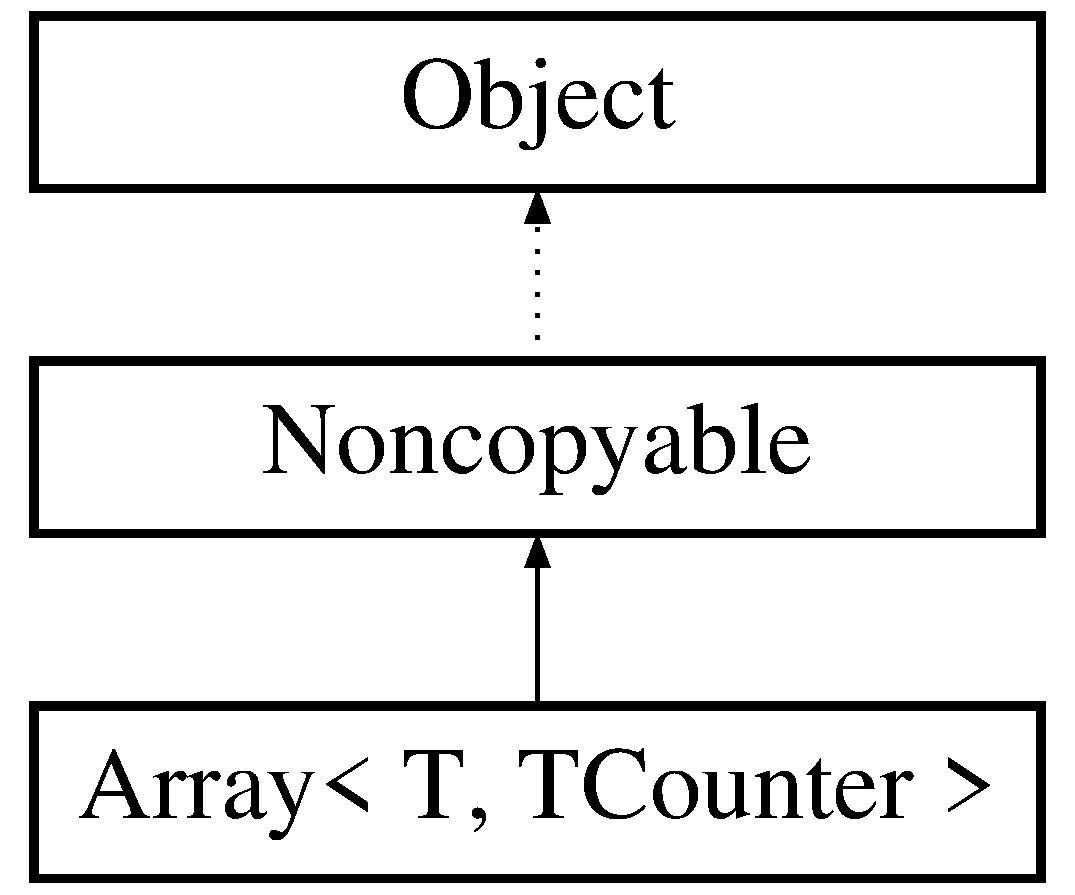
\includegraphics[height=3.000000cm]{classArray}
\end{center}
\end{figure}
\subsection*{Public Types}
\begin{DoxyCompactItemize}
\item 
\hypertarget{classArray_abe06e3ce546d101b3ccf2b1398445a1a}{}\label{classArray_abe06e3ce546d101b3ccf2b1398445a1a} 
using {\bfseries Type} = T
\end{DoxyCompactItemize}
\subsection*{Public Member Functions}
\begin{DoxyCompactItemize}
\item 
\hyperlink{classArray_a53a67b010c774165bbf8b64e1d4ee0e2}{Array} (const T\+Counter element\+Cnt, const T\+Counter allocated\+Size=-\/1)
\item 
\hyperlink{classArray_a4f87480b3f5553c15c70ddad372602fd}{Array} (std\+::initializer\+\_\+list$<$ T $>$ list)
\item 
\hypertarget{classArray_adbb5bab1e50f7b4728052f2a98eff126}{}\label{classArray_adbb5bab1e50f7b4728052f2a98eff126} 
\hyperlink{classArray_adbb5bab1e50f7b4728052f2a98eff126}{Array} (\hyperlink{classArray}{Array} \&\&other)
\begin{DoxyCompactList}\small\item\em Move constructor. \end{DoxyCompactList}\item 
\hypertarget{classArray_a675694cfa6441f7c138df7a9f20979a3}{}\label{classArray_a675694cfa6441f7c138df7a9f20979a3} 
\hyperlink{classArray_a675694cfa6441f7c138df7a9f20979a3}{$\sim$\+Array} ()
\begin{DoxyCompactList}\small\item\em Destructor. \end{DoxyCompactList}\item 
\hypertarget{classArray_a441d346a10b575c0a5989df056d9a96f}{}\label{classArray_a441d346a10b575c0a5989df056d9a96f} 
\hyperlink{classArray}{Array} \& \hyperlink{classArray_a441d346a10b575c0a5989df056d9a96f}{operator=} (\hyperlink{classArray}{Array} \&\&other)
\begin{DoxyCompactList}\small\item\em Move operator. \end{DoxyCompactList}\item 
\hyperlink{classArray}{Array} \hyperlink{classArray_a7cb2b9b74ad6856612d0bfcdbb0be366}{clone} () const
\item 
\hypertarget{classArray_a54fb6bf131beb33ac622f86ea69b8252}{}\label{classArray_a54fb6bf131beb33ac622f86ea69b8252} 
\hyperlink{classIterator}{Iterator}$<$ T, T\+Counter $>$ {\bfseries begin} ()
\item 
\hypertarget{classArray_a1298de4f3c86cc976c4a8e96bd9f5526}{}\label{classArray_a1298de4f3c86cc976c4a8e96bd9f5526} 
\hyperlink{classIterator}{Iterator}$<$ const T, T\+Counter $>$ {\bfseries begin} () const
\item 
\hypertarget{classArray_a751a6999d94a005be83344c131196ac4}{}\label{classArray_a751a6999d94a005be83344c131196ac4} 
\hyperlink{classIterator}{Iterator}$<$ const T, T\+Counter $>$ {\bfseries cbegin} () const
\item 
\hypertarget{classArray_a79f668040fdf1ecf120ea8b2e5084190}{}\label{classArray_a79f668040fdf1ecf120ea8b2e5084190} 
\hyperlink{classIterator}{Iterator}$<$ T, T\+Counter $>$ {\bfseries end} ()
\item 
\hypertarget{classArray_ab607b1de02960ec3f282526be9aa1afc}{}\label{classArray_ab607b1de02960ec3f282526be9aa1afc} 
\hyperlink{classIterator}{Iterator}$<$ const T, T\+Counter $>$ {\bfseries end} () const
\item 
\hypertarget{classArray_afafcc1c1eb0da2e56e5a37a1456d9cb4}{}\label{classArray_afafcc1c1eb0da2e56e5a37a1456d9cb4} 
\hyperlink{classIterator}{Iterator}$<$ const T, T\+Counter $>$ {\bfseries cend} () const
\item 
\hypertarget{classArray_a8829af2d483c4e9ee2269a5deee6f042}{}\label{classArray_a8829af2d483c4e9ee2269a5deee6f042} 
T \& {\bfseries operator\mbox{[}$\,$\mbox{]}} (const T\+Counter idx)
\item 
\hypertarget{classArray_ad2d84eb9a3cd270c134ee915b280a27d}{}\label{classArray_ad2d84eb9a3cd270c134ee915b280a27d} 
const T \& {\bfseries operator\mbox{[}$\,$\mbox{]}} (const T\+Counter idx) const
\item 
\hypertarget{classArray_ad1690497f80539c2a92357d65b9a9d66}{}\label{classArray_ad1690497f80539c2a92357d65b9a9d66} 
void {\bfseries fill} (const T \&t)
\item 
\hypertarget{classArray_a02fc8237ecb8bd11ad35ec01824dfdcf}{}\label{classArray_a02fc8237ecb8bd11ad35ec01824dfdcf} 
int {\bfseries get\+Size} () const
\item 
\hypertarget{classArray_a6e420323d0af017e30f643876aecd0a6}{}\label{classArray_a6e420323d0af017e30f643876aecd0a6} 
bool {\bfseries is\+Empty} () const
\item 
\hypertarget{classArray_a790180f66bcedec3a38db50c2fadd84b}{}\label{classArray_a790180f66bcedec3a38db50c2fadd84b} 
void \hyperlink{classArray_a790180f66bcedec3a38db50c2fadd84b}{resize} (const int new\+Size)
\begin{DoxyCompactList}\small\item\em Resize the array. All stored values (within interval \mbox{[}0, new\+Size-\/1\mbox{]}) are preserved. \end{DoxyCompactList}\item 
\hypertarget{classArray_a1e86cc82e0f42858019f53d32b199b12}{}\label{classArray_a1e86cc82e0f42858019f53d32b199b12} 
{\footnotesize template$<$typename U $>$ }\\void \hyperlink{classArray_a1e86cc82e0f42858019f53d32b199b12}{push} (U \&\&u)
\begin{DoxyCompactList}\small\item\em Adds new element to the end of the array, resizing the array if necessary. \end{DoxyCompactList}\item 
\hypertarget{classArray_a5797217fb33af6d856c540a0bce23cc1}{}\label{classArray_a5797217fb33af6d856c540a0bce23cc1} 
{\footnotesize template$<$typename U $>$ }\\void {\bfseries push\+All} (const \hyperlink{classIterator}{Iterator}$<$ const U $>$ first, const \hyperlink{classIterator}{Iterator}$<$ const U $>$ last)
\item 
\hypertarget{classArray_adeead0fb323a28435fa16a6fe13559d1}{}\label{classArray_adeead0fb323a28435fa16a6fe13559d1} 
void {\bfseries push\+All} (const \hyperlink{classArray}{Array} \&other)
\item 
\hypertarget{classArray_a0ba794d2239817cfeed5512599eb6679}{}\label{classArray_a0ba794d2239817cfeed5512599eb6679} 
T \hyperlink{classArray_a0ba794d2239817cfeed5512599eb6679}{pop} ()
\begin{DoxyCompactList}\small\item\em Removes the last element from the array and return its value. Asserts if the array is empty. \end{DoxyCompactList}\item 
\hypertarget{classArray_ad36b577886afcb82a3c744c3339d2adb}{}\label{classArray_ad36b577886afcb82a3c744c3339d2adb} 
void \hyperlink{classArray_ad36b577886afcb82a3c744c3339d2adb}{clear} ()
\begin{DoxyCompactList}\small\item\em Removes all elements from the array, but does N\+OT release the memory. \end{DoxyCompactList}\item 
\hypertarget{classArray_a99b7e81488b19f5469572ed8a89701cb}{}\label{classArray_a99b7e81488b19f5469572ed8a89701cb} 
\hyperlink{classArray_a99b7e81488b19f5469572ed8a89701cb}{operator Array\+View$<$ T, T\+Counter $>$} ()
\begin{DoxyCompactList}\small\item\em Implicit conversion to arrayview. \end{DoxyCompactList}\item 
\hypertarget{classArray_ab2c82ba3fe89a0eb1e263cced745ce25}{}\label{classArray_ab2c82ba3fe89a0eb1e263cced745ce25} 
\hyperlink{classArray_ab2c82ba3fe89a0eb1e263cced745ce25}{operator Array\+View$<$ const T, T\+Counter $>$} () const
\begin{DoxyCompactList}\small\item\em Implicit conversion to arrayview, const version. \end{DoxyCompactList}\item 
bool \hyperlink{classArray_a7eff7030d460a572a7076f2ed2464448}{operator==} (const \hyperlink{classArray}{Array}$<$ T, T\+Counter $>$ \&other) const
\end{DoxyCompactItemize}


\subsection{Constructor \& Destructor Documentation}
\hypertarget{classArray_a53a67b010c774165bbf8b64e1d4ee0e2}{}\label{classArray_a53a67b010c774165bbf8b64e1d4ee0e2} 
\index{Array@{Array}!Array@{Array}}
\index{Array@{Array}!Array@{Array}}
\subsubsection{\texorpdfstring{Array()}{Array()}\hspace{0.1cm}{\footnotesize\ttfamily [1/2]}}
{\footnotesize\ttfamily template$<$typename T, typename T\+Counter = int$>$ \\
\hyperlink{classArray}{Array}$<$ T, T\+Counter $>$\+::\hyperlink{classArray}{Array} (\begin{DoxyParamCaption}\item[{const T\+Counter}]{element\+Cnt,  }\item[{const T\+Counter}]{allocated\+Size = {\ttfamily -\/1} }\end{DoxyParamCaption})\hspace{0.3cm}{\ttfamily [inline]}, {\ttfamily [explicit]}}

Constructs array of given size. 
\begin{DoxyParams}{Parameters}
{\em element\+Cnt} & Number of elements to be constructed (using default constructor) \\
\hline
{\em allocated\+Size} & Number of allocated elements. \\
\hline
\end{DoxyParams}
\hypertarget{classArray_a4f87480b3f5553c15c70ddad372602fd}{}\label{classArray_a4f87480b3f5553c15c70ddad372602fd} 
\index{Array@{Array}!Array@{Array}}
\index{Array@{Array}!Array@{Array}}
\subsubsection{\texorpdfstring{Array()}{Array()}\hspace{0.1cm}{\footnotesize\ttfamily [2/2]}}
{\footnotesize\ttfamily template$<$typename T, typename T\+Counter = int$>$ \\
\hyperlink{classArray}{Array}$<$ T, T\+Counter $>$\+::\hyperlink{classArray}{Array} (\begin{DoxyParamCaption}\item[{std\+::initializer\+\_\+list$<$ T $>$}]{list }\end{DoxyParamCaption})\hspace{0.3cm}{\ttfamily [inline]}}

Constructs array from initialized list. Allocate only enough elements to store the list. Elements are constructed using copy constructor of stored type. 

\subsection{Member Function Documentation}
\hypertarget{classArray_a7cb2b9b74ad6856612d0bfcdbb0be366}{}\label{classArray_a7cb2b9b74ad6856612d0bfcdbb0be366} 
\index{Array@{Array}!clone@{clone}}
\index{clone@{clone}!Array@{Array}}
\subsubsection{\texorpdfstring{clone()}{clone()}}
{\footnotesize\ttfamily template$<$typename T, typename T\+Counter = int$>$ \\
\hyperlink{classArray}{Array} \hyperlink{classArray}{Array}$<$ T, T\+Counter $>$\+::clone (\begin{DoxyParamCaption}{ }\end{DoxyParamCaption}) const\hspace{0.3cm}{\ttfamily [inline]}}

Copy method -- allow to copy array only with an explicit calling of \textquotesingle{}clone\textquotesingle{} to avoid accidental deep copy. \hypertarget{classArray_a7eff7030d460a572a7076f2ed2464448}{}\label{classArray_a7eff7030d460a572a7076f2ed2464448} 
\index{Array@{Array}!operator==@{operator==}}
\index{operator==@{operator==}!Array@{Array}}
\subsubsection{\texorpdfstring{operator==()}{operator==()}}
{\footnotesize\ttfamily template$<$typename T, typename T\+Counter = int$>$ \\
bool \hyperlink{classArray}{Array}$<$ T, T\+Counter $>$\+::operator== (\begin{DoxyParamCaption}\item[{const \hyperlink{classArray}{Array}$<$ T, T\+Counter $>$ \&}]{other }\end{DoxyParamCaption}) const\hspace{0.3cm}{\ttfamily [inline]}}

Comparison operator, comparings array element-\/by-\/element. If arrays differ in number of constructed elements, the comparison always returns false; allocated size does not play role here. 

The documentation for this class was generated from the following file\+:\begin{DoxyCompactItemize}
\item 
/home/pavel/projects/astro/sph2/src/structs/array.\+h\end{DoxyCompactItemize}

\hypertarget{structSph_1_1array__or__vector__selector}{}\section{Sph\+:\+:array\+\_\+or\+\_\+vector\+\_\+selector$<$ D\+IM, T $>$ Struct Template Reference}
\label{structSph_1_1array__or__vector__selector}\index{Sph\+::array\+\_\+or\+\_\+vector\+\_\+selector$<$ D\+I\+M, T $>$@{Sph\+::array\+\_\+or\+\_\+vector\+\_\+selector$<$ D\+I\+M, T $>$}}


{\ttfamily \#include $<$nanoflann.\+h$>$}

\subsection*{Public Types}
\begin{DoxyCompactItemize}
\item 
\hypertarget{structSph_1_1array__or__vector__selector_af60a03c0f085e18f62638e8221fd2954}{}\label{structSph_1_1array__or__vector__selector_af60a03c0f085e18f62638e8221fd2954} 
typedef \hyperlink{classSph_1_1CArray}{C\+Array}$<$ T, D\+IM $>$ {\bfseries container\+\_\+t}
\end{DoxyCompactItemize}


\subsection{Detailed Description}
\subsubsection*{template$<$int D\+IM, typename T$>$\newline
struct Sph\+::array\+\_\+or\+\_\+vector\+\_\+selector$<$ D\+I\+M, T $>$}

Used to declare fixed-\/size arrays when D\+IM$>$0, dynamically-\/allocated vectors when D\+IM=-\/1. Fixed size version for a generic D\+IM\+: 

The documentation for this struct was generated from the following file\+:\begin{DoxyCompactItemize}
\item 
/home/pavel/projects/astro/sph2/src/tree/nanoflann.\+h\end{DoxyCompactItemize}

\hypertarget{structSph_1_1array__or__vector__selector_3-1_00_01T_01_4}{}\section{Sph\+:\+:array\+\_\+or\+\_\+vector\+\_\+selector$<$-\/1, T $>$ Struct Template Reference}
\label{structSph_1_1array__or__vector__selector_3-1_00_01T_01_4}\index{Sph\+::array\+\_\+or\+\_\+vector\+\_\+selector$<$-\/1, T $>$@{Sph\+::array\+\_\+or\+\_\+vector\+\_\+selector$<$-\/1, T $>$}}


{\ttfamily \#include $<$nanoflann.\+h$>$}

\subsection*{Public Types}
\begin{DoxyCompactItemize}
\item 
\hypertarget{structSph_1_1array__or__vector__selector_3-1_00_01T_01_4_a9459fb133d60702c309ec1c5522f2053}{}\label{structSph_1_1array__or__vector__selector_3-1_00_01T_01_4_a9459fb133d60702c309ec1c5522f2053} 
typedef \hyperlink{classArray}{Array}$<$ T $>$ {\bfseries container\+\_\+t}
\end{DoxyCompactItemize}


\subsection{Detailed Description}
\subsubsection*{template$<$typename T$>$\newline
struct Sph\+::array\+\_\+or\+\_\+vector\+\_\+selector$<$-\/1, T $>$}

Dynamic size version 

The documentation for this struct was generated from the following file\+:\begin{DoxyCompactItemize}
\item 
/home/pavel/projects/astro/sph2/src/tree/nanoflann.\+h\end{DoxyCompactItemize}

\hypertarget{classArrayView}{}\section{Array\+View$<$ T, T\+Counter $>$ Class Template Reference}
\label{classArrayView}\index{Array\+View$<$ T, T\+Counter $>$@{Array\+View$<$ T, T\+Counter $>$}}
Inheritance diagram for Array\+View$<$ T, T\+Counter $>$\+:\begin{figure}[H]
\begin{center}
\leavevmode
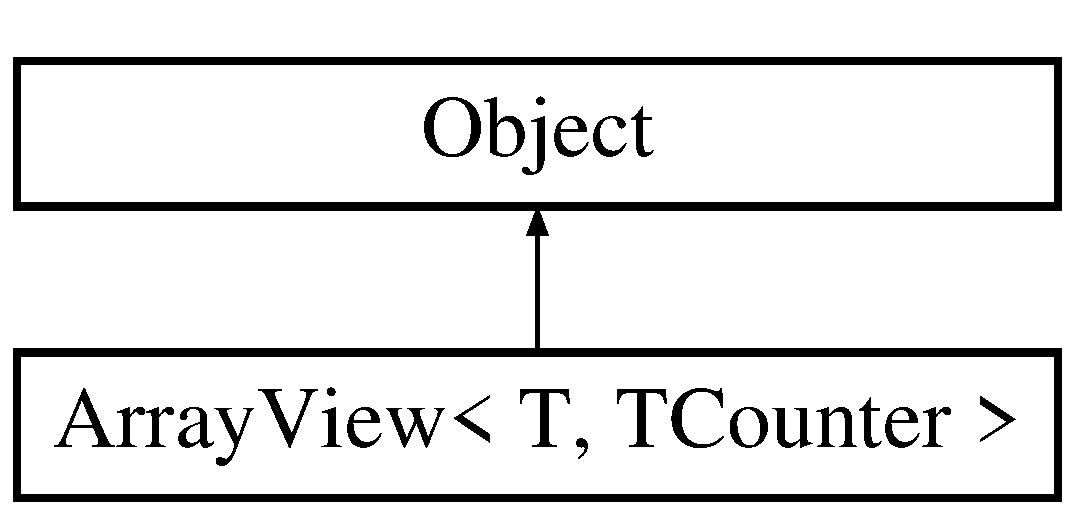
\includegraphics[height=2.000000cm]{classArrayView}
\end{center}
\end{figure}
\subsection*{Public Member Functions}
\begin{DoxyCompactItemize}
\item 
\hypertarget{classArrayView_aa48aec8978420bc5a9d6d99f8c0f5d89}{}\label{classArrayView_aa48aec8978420bc5a9d6d99f8c0f5d89} 
{\bfseries Array\+View} (T $\ast$data, T\+Counter size)
\item 
\hypertarget{classArrayView_a4698fee2b1061a1566c8c46dccb799bb}{}\label{classArrayView_a4698fee2b1061a1566c8c46dccb799bb} 
{\bfseries Array\+View} (std\+::initializer\+\_\+list$<$ T $>$ list)
\item 
\hypertarget{classArrayView_a67c0cd88e7a636210f9a9be2f1a23cd4}{}\label{classArrayView_a67c0cd88e7a636210f9a9be2f1a23cd4} 
{\bfseries Array\+View} (const \hyperlink{classArrayView}{Array\+View} \&other)
\item 
\hypertarget{classArrayView_a43488b273e526426af792e81769d98e6}{}\label{classArrayView_a43488b273e526426af792e81769d98e6} 
\hyperlink{classArrayView_a43488b273e526426af792e81769d98e6}{Array\+View} (\hyperlink{classArrayView}{Array\+View} \&\&other)
\begin{DoxyCompactList}\small\item\em Move constructor. \end{DoxyCompactList}\item 
\hypertarget{classArrayView_a10028583b4df8d21bb2b411aa12dc698}{}\label{classArrayView_a10028583b4df8d21bb2b411aa12dc698} 
\hyperlink{classArrayView}{Array\+View} \& \hyperlink{classArrayView_a10028583b4df8d21bb2b411aa12dc698}{operator=} (const \hyperlink{classArrayView}{Array\+View} \&other)
\begin{DoxyCompactList}\small\item\em Copy operator. \end{DoxyCompactList}\item 
\hypertarget{classArrayView_aae5ed0dd43b799f8d1f6f7d794cc4715}{}\label{classArrayView_aae5ed0dd43b799f8d1f6f7d794cc4715} 
\hyperlink{classArrayView}{Array\+View} \& \hyperlink{classArrayView_aae5ed0dd43b799f8d1f6f7d794cc4715}{operator=} (\hyperlink{classArrayView}{Array\+View} \&\&other)
\begin{DoxyCompactList}\small\item\em Move operator. \end{DoxyCompactList}\item 
\hypertarget{classArrayView_a9ce305091383c594f125c8cf312c6bf6}{}\label{classArrayView_a9ce305091383c594f125c8cf312c6bf6} 
\hyperlink{classIterator}{Iterator}$<$ T, T\+Counter $>$ {\bfseries begin} ()
\item 
\hypertarget{classArrayView_a36d4ca146561aa28a34cd1dab265bfa7}{}\label{classArrayView_a36d4ca146561aa28a34cd1dab265bfa7} 
\hyperlink{classIterator}{Iterator}$<$ const T, T\+Counter $>$ {\bfseries begin} () const
\item 
\hypertarget{classArrayView_a4b45a5022db66eb8756e6fa367ec2b43}{}\label{classArrayView_a4b45a5022db66eb8756e6fa367ec2b43} 
\hyperlink{classIterator}{Iterator}$<$ T, T\+Counter $>$ {\bfseries end} ()
\item 
\hypertarget{classArrayView_a53614bd711745a629ba1610aa0a54b71}{}\label{classArrayView_a53614bd711745a629ba1610aa0a54b71} 
\hyperlink{classIterator}{Iterator}$<$ const T, T\+Counter $>$ {\bfseries end} () const
\item 
\hypertarget{classArrayView_afecc27ee9a9ee1ee5b8f8f2328957ad7}{}\label{classArrayView_afecc27ee9a9ee1ee5b8f8f2328957ad7} 
T \& {\bfseries operator\mbox{[}$\,$\mbox{]}} (const T\+Counter idx)
\item 
\hypertarget{classArrayView_a4004286643a5488b4696fbabac87b785}{}\label{classArrayView_a4004286643a5488b4696fbabac87b785} 
const T \& {\bfseries operator\mbox{[}$\,$\mbox{]}} (const T\+Counter idx) const
\item 
\hypertarget{classArrayView_abbb0ed5009a3070dff94fb9545c96843}{}\label{classArrayView_abbb0ed5009a3070dff94fb9545c96843} 
int {\bfseries get\+Size} () const
\end{DoxyCompactItemize}


The documentation for this class was generated from the following file\+:\begin{DoxyCompactItemize}
\item 
/home/pavel/projects/astro/sph2/src/structs/arrayview.\+h\end{DoxyCompactItemize}

\hypertarget{structBaseType}{}\section{Base\+Type$<$ T\+Unit $>$ Struct Template Reference}
\label{structBaseType}\index{Base\+Type$<$ T\+Unit $>$@{Base\+Type$<$ T\+Unit $>$}}


{\ttfamily \#include $<$traits.\+h$>$}

\subsection*{Public Types}
\begin{DoxyCompactItemize}
\item 
\hypertarget{structBaseType_a2d02b49267d883c4aabbfa503c3e16bf}{}\label{structBaseType_a2d02b49267d883c4aabbfa503c3e16bf} 
using {\bfseries Type} = T\+Unit
\end{DoxyCompactItemize}


\subsection{Detailed Description}
\subsubsection*{template$<$typename T\+Unit$>$\newline
struct Base\+Type$<$ T\+Unit $>$}

Base type of the quantity By default, it is the type of the quantity itself For units, it is the type of the value. 

The documentation for this struct was generated from the following file\+:\begin{DoxyCompactItemize}
\item 
/home/pavel/projects/astro/sph2/src/core/traits.\+h\end{DoxyCompactItemize}

\hypertarget{classBasicIndices}{}\section{Basic\+Indices$<$ T $>$ Class Template Reference}
\label{classBasicIndices}\index{Basic\+Indices$<$ T $>$@{Basic\+Indices$<$ T $>$}}


{\ttfamily \#include $<$indices.\+h$>$}

Inheritance diagram for Basic\+Indices$<$ T $>$\+:\begin{figure}[H]
\begin{center}
\leavevmode
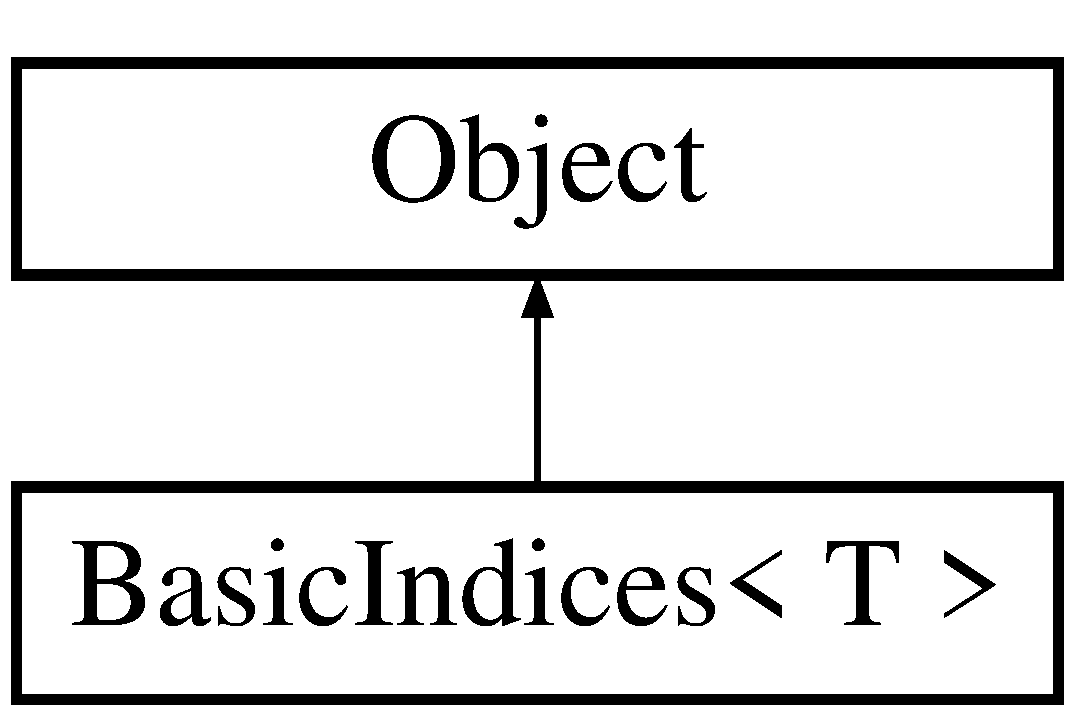
\includegraphics[height=2.000000cm]{classBasicIndices}
\end{center}
\end{figure}
\subsection*{Public Member Functions}
\begin{DoxyCompactItemize}
\item 
\hypertarget{classBasicIndices_a6a8c243116832f0238d8c1f1bf3add9e}{}\label{classBasicIndices_a6a8c243116832f0238d8c1f1bf3add9e} 
\hyperlink{classBasicIndices_a6a8c243116832f0238d8c1f1bf3add9e}{Basic\+Indices} (ValueT i, ValueT j, ValueT k, ValueT l=\hyperlink{classDummyReferenceMaker}{DummyT}())
\begin{DoxyCompactList}\small\item\em Constructs indices from values. Fourth component is optional. \end{DoxyCompactList}\item 
\hypertarget{classBasicIndices_ad717c49ee83f41609a3ffdb36375e1f8}{}\label{classBasicIndices_ad717c49ee83f41609a3ffdb36375e1f8} 
{\footnotesize template$<$typename T\+Other  = T, typename  = std\+::enable\+\_\+if\+\_\+t$<$!std\+::is\+\_\+reference$<$\+T$>$\+::value, T\+Other$>$$>$ }\\\hyperlink{classBasicIndices_ad717c49ee83f41609a3ffdb36375e1f8}{Basic\+Indices} (const \hyperlink{classBasicIndices}{Basic\+Indices}$<$ T\+Other $>$ \&other)
\begin{DoxyCompactList}\small\item\em Copy constructor from const indices. \end{DoxyCompactList}\item 
\hypertarget{classBasicIndices_ac75e8f4b9e0f1cb72612047d792c85c2}{}\label{classBasicIndices_ac75e8f4b9e0f1cb72612047d792c85c2} 
{\footnotesize template$<$typename T\+Other  = T, typename  = std\+::enable\+\_\+if\+\_\+t$<$std\+::is\+\_\+reference$<$\+T$>$\+::value, T\+Other$>$$>$ }\\\hyperlink{classBasicIndices_ac75e8f4b9e0f1cb72612047d792c85c2}{Basic\+Indices} (\hyperlink{classBasicIndices}{Basic\+Indices}$<$ T\+Other $>$ \&other)
\begin{DoxyCompactList}\small\item\em Copy constructor from l-\/value reference, enabled only for reference underlying type. \end{DoxyCompactList}\item 
\hypertarget{classBasicIndices_a196c3849d76701f87cfe9c5f08be80e4}{}\label{classBasicIndices_a196c3849d76701f87cfe9c5f08be80e4} 
{\footnotesize template$<$typename T\+Other , typename  = std\+::enable\+\_\+if\+\_\+t$<$std\+::is\+\_\+reference$<$\+T$>$\+::value, T\+Other$>$$>$ }\\\hyperlink{classBasicIndices}{Basic\+Indices} \& {\bfseries operator=} (\hyperlink{classBasicIndices}{Basic\+Indices}$<$ T\+Other $>$ \&other)
\item 
\hypertarget{classBasicIndices_a97d894fe77b1a4f7c3013c776493afee}{}\label{classBasicIndices_a97d894fe77b1a4f7c3013c776493afee} 
{\footnotesize template$<$typename T\+Other $>$ }\\\hyperlink{classBasicIndices}{Basic\+Indices} \& {\bfseries operator=} (const \hyperlink{classBasicIndices}{Basic\+Indices}$<$ T\+Other $>$ \&other)
\item 
\hypertarget{classBasicIndices_a55d907b78f920f2efef89ec3bff9f049}{}\label{classBasicIndices_a55d907b78f920f2efef89ec3bff9f049} 
RawT \& {\bfseries operator\mbox{[}$\,$\mbox{]}} (const int idx)
\item 
\hypertarget{classBasicIndices_a9c2765925b94da3113252c1ed635a403}{}\label{classBasicIndices_a9c2765925b94da3113252c1ed635a403} 
const RawT \& {\bfseries operator\mbox{[}$\,$\mbox{]}} (const int idx) const
\item 
\hypertarget{classBasicIndices_ac9efe24f22d605f8367f8117b4f858cf}{}\label{classBasicIndices_ac9efe24f22d605f8367f8117b4f858cf} 
bool {\bfseries operator==} (const \hyperlink{classBasicIndices}{Basic\+Indices} \&other)
\item 
\hypertarget{classBasicIndices_af1f37a4b1783447d0e38a5f24ed03285}{}\label{classBasicIndices_af1f37a4b1783447d0e38a5f24ed03285} 
bool {\bfseries operator!=} (const \hyperlink{classBasicIndices}{Basic\+Indices} \&other)
\end{DoxyCompactItemize}
\subsection*{Friends}
\begin{DoxyCompactItemize}
\item 
\hypertarget{classBasicIndices_a55d7587dc9fcfcc78c838f1401417738}{}\label{classBasicIndices_a55d7587dc9fcfcc78c838f1401417738} 
{\footnotesize template$<$typename $>$ }\\class {\bfseries Basic\+Indices}
\item 
\hypertarget{classBasicIndices_a4bfdb985aa6c2005116deaa410c26a98}{}\label{classBasicIndices_a4bfdb985aa6c2005116deaa410c26a98} 
{\footnotesize template$<$typename T\+Stream $>$ }\\T\+Stream \& {\bfseries operator$<$$<$} (T\+Stream \&stream, const \hyperlink{classBasicIndices}{Basic\+Indices} \&indices)
\end{DoxyCompactItemize}


\subsection{Detailed Description}
\subsubsection*{template$<$typename T$>$\newline
class Basic\+Indices$<$ T $>$}

\begin{DoxyRefDesc}{Todo}
\item[\hyperlink{todo__todo000008}{Todo}]specialize for non-\/ref types? For reference types, the fourth component is still optional. If not used, however, getting the value will access memory of destroyed temporary object and result in crash, the safety is left to the user. \end{DoxyRefDesc}


The documentation for this class was generated from the following file\+:\begin{DoxyCompactItemize}
\item 
/home/pavel/projects/astro/sph2/src/geometry/indices.\+h\end{DoxyCompactItemize}

\hypertarget{classBasicVector}{}\section{Basic\+Vector$<$ T $>$ Class Template Reference}
\label{classBasicVector}\index{Basic\+Vector$<$ T $>$@{Basic\+Vector$<$ T $>$}}


The documentation for this class was generated from the following file\+:\begin{DoxyCompactItemize}
\item 
/home/pavel/projects/astro/sph2/src/geometry/vector.\+h\end{DoxyCompactItemize}

\hypertarget{classBasicVector_3_01double_01_4}{}\section{Basic\+Vector$<$ double $>$ Class Template Reference}
\label{classBasicVector_3_01double_01_4}\index{Basic\+Vector$<$ double $>$@{Basic\+Vector$<$ double $>$}}
Inheritance diagram for Basic\+Vector$<$ double $>$\+:\begin{figure}[H]
\begin{center}
\leavevmode
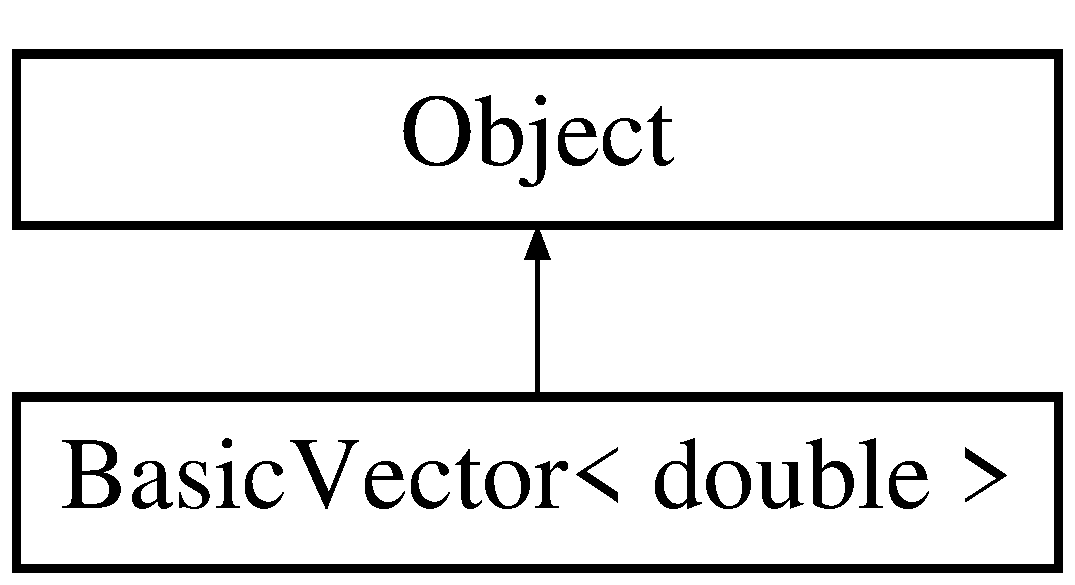
\includegraphics[height=2.000000cm]{classBasicVector_3_01double_01_4}
\end{center}
\end{figure}
\subsection*{Public Member Functions}
\begin{DoxyCompactItemize}
\item 
\hypertarget{classBasicVector_3_01double_01_4_a889c95ee2545471163f55487b033de91}{}\label{classBasicVector_3_01double_01_4_a889c95ee2545471163f55487b033de91} 
I\+N\+L\+I\+NE \hyperlink{classBasicVector_3_01double_01_4_a889c95ee2545471163f55487b033de91}{Basic\+Vector} (const \+\_\+\+\_\+m256d data)
\begin{DoxyCompactList}\small\item\em Constructs from S\+SE vector. \end{DoxyCompactList}\item 
\hypertarget{classBasicVector_3_01double_01_4_a4986ebfd741106b6321a8b94fd06f250}{}\label{classBasicVector_3_01double_01_4_a4986ebfd741106b6321a8b94fd06f250} 
I\+N\+L\+I\+NE \hyperlink{classBasicVector_3_01double_01_4_a4986ebfd741106b6321a8b94fd06f250}{Basic\+Vector} (const double f)
\begin{DoxyCompactList}\small\item\em Constructs by copying a value to all vector components. \end{DoxyCompactList}\item 
\hypertarget{classBasicVector_3_01double_01_4_a342f3502c1fa844d0a652fbe32cda072}{}\label{classBasicVector_3_01double_01_4_a342f3502c1fa844d0a652fbe32cda072} 
I\+N\+L\+I\+NE \hyperlink{classBasicVector_3_01double_01_4_a342f3502c1fa844d0a652fbe32cda072}{Basic\+Vector} (const double x, const double y, const double z=0., const double h=0.)
\begin{DoxyCompactList}\small\item\em Constructs the vector from given components. \end{DoxyCompactList}\item 
\hypertarget{classBasicVector_3_01double_01_4_a0f92a97b290b5fa81170e2989aa6ac97}{}\label{classBasicVector_3_01double_01_4_a0f92a97b290b5fa81170e2989aa6ac97} 
I\+N\+L\+I\+NE \hyperlink{classBasicVector_3_01double_01_4_a0f92a97b290b5fa81170e2989aa6ac97}{Basic\+Vector} (const \hyperlink{classBasicVector}{Basic\+Vector} \&v)
\begin{DoxyCompactList}\small\item\em Copy constructor. \end{DoxyCompactList}\item 
\hypertarget{classBasicVector_3_01double_01_4_a452d8ac00f2c7176d13512bbac155c57}{}\label{classBasicVector_3_01double_01_4_a452d8ac00f2c7176d13512bbac155c57} 
I\+N\+L\+I\+NE \hyperlink{classBasicVector_3_01double_01_4_a452d8ac00f2c7176d13512bbac155c57}{Basic\+Vector} (\hyperlink{classBasicVector}{Basic\+Vector} \&\&v)
\begin{DoxyCompactList}\small\item\em Move constructor. \end{DoxyCompactList}\item 
\hypertarget{classBasicVector_3_01double_01_4_a80108c25a1f3a10f964e75e6e3105f0d}{}\label{classBasicVector_3_01double_01_4_a80108c25a1f3a10f964e75e6e3105f0d} 
I\+N\+L\+I\+NE const double \& \hyperlink{classBasicVector_3_01double_01_4_a80108c25a1f3a10f964e75e6e3105f0d}{operator\mbox{[}$\,$\mbox{]}} (const int i) const
\begin{DoxyCompactList}\small\item\em Get component by given index. \end{DoxyCompactList}\item 
\hypertarget{classBasicVector_3_01double_01_4_af046e4e752d917e083d77dbd66bf6f93}{}\label{classBasicVector_3_01double_01_4_af046e4e752d917e083d77dbd66bf6f93} 
I\+N\+L\+I\+NE double \& \hyperlink{classBasicVector_3_01double_01_4_af046e4e752d917e083d77dbd66bf6f93}{operator\mbox{[}$\,$\mbox{]}} (const int i)
\begin{DoxyCompactList}\small\item\em Get component by given index. \end{DoxyCompactList}\item 
\hypertarget{classBasicVector_3_01double_01_4_aa3e0eb8159a00bef3fd587e212bf8fb1}{}\label{classBasicVector_3_01double_01_4_aa3e0eb8159a00bef3fd587e212bf8fb1} 
{\footnotesize template$<$int i$>$ }\\I\+N\+L\+I\+NE const double \& \hyperlink{classBasicVector_3_01double_01_4_aa3e0eb8159a00bef3fd587e212bf8fb1}{get} () const
\begin{DoxyCompactList}\small\item\em Get component by given compile-\/time constant index. \end{DoxyCompactList}\item 
\hypertarget{classBasicVector_3_01double_01_4_a6b1022e55f898c344599ae494f61d733}{}\label{classBasicVector_3_01double_01_4_a6b1022e55f898c344599ae494f61d733} 
{\footnotesize template$<$int i$>$ }\\I\+N\+L\+I\+NE double \& \hyperlink{classBasicVector_3_01double_01_4_a6b1022e55f898c344599ae494f61d733}{get} ()
\begin{DoxyCompactList}\small\item\em Get component by given compile-\/time constant index. \end{DoxyCompactList}\item 
\hypertarget{classBasicVector_3_01double_01_4_a11157f9400a7706ec87a967892019359}{}\label{classBasicVector_3_01double_01_4_a11157f9400a7706ec87a967892019359} 
I\+N\+L\+I\+NE \hyperlink{classBasicVector}{Basic\+Vector} \& \hyperlink{classBasicVector_3_01double_01_4_a11157f9400a7706ec87a967892019359}{operator=} (const \hyperlink{classBasicVector}{Basic\+Vector} \&v)
\begin{DoxyCompactList}\small\item\em Copy operator. \end{DoxyCompactList}\item 
\hypertarget{classBasicVector_3_01double_01_4_ace68123af6c89d86318d13683e5f4eea}{}\label{classBasicVector_3_01double_01_4_ace68123af6c89d86318d13683e5f4eea} 
I\+N\+L\+I\+NE \hyperlink{classBasicVector}{Basic\+Vector} \& \hyperlink{classBasicVector_3_01double_01_4_ace68123af6c89d86318d13683e5f4eea}{operator=} (\hyperlink{classBasicVector}{Basic\+Vector} \&\&v)
\begin{DoxyCompactList}\small\item\em Move operator. \end{DoxyCompactList}\item 
\hypertarget{classBasicVector_3_01double_01_4_a01a354b7eaf0142a7f41794d407dd6ae}{}\label{classBasicVector_3_01double_01_4_a01a354b7eaf0142a7f41794d407dd6ae} 
I\+N\+L\+I\+NE \hyperlink{classBasicVector}{Basic\+Vector} \& {\bfseries operator+=} (const \hyperlink{classBasicVector}{Basic\+Vector} \&v)
\item 
\hypertarget{classBasicVector_3_01double_01_4_acebdc955cc10f605ca85be4cc725bb79}{}\label{classBasicVector_3_01double_01_4_acebdc955cc10f605ca85be4cc725bb79} 
I\+N\+L\+I\+NE \hyperlink{classBasicVector}{Basic\+Vector} \& {\bfseries operator-\/=} (const \hyperlink{classBasicVector}{Basic\+Vector} \&v)
\item 
\hypertarget{classBasicVector_3_01double_01_4_a19abfac47ea052e2f00f8da97c9053c7}{}\label{classBasicVector_3_01double_01_4_a19abfac47ea052e2f00f8da97c9053c7} 
I\+N\+L\+I\+NE \hyperlink{classBasicVector}{Basic\+Vector} \& {\bfseries operator$\ast$=} (const double f)
\item 
\hypertarget{classBasicVector_3_01double_01_4_ac509c2608313557664c8a8690ffe1384}{}\label{classBasicVector_3_01double_01_4_ac509c2608313557664c8a8690ffe1384} 
I\+N\+L\+I\+NE \hyperlink{classBasicVector}{Basic\+Vector} \& {\bfseries operator/=} (const double f)
\item 
\hypertarget{classBasicVector_3_01double_01_4_a316cd710c684228f8bd37615cd54ed8f}{}\label{classBasicVector_3_01double_01_4_a316cd710c684228f8bd37615cd54ed8f} 
I\+N\+L\+I\+NE \hyperlink{classBasicVector}{Basic\+Vector} \& {\bfseries operator$\ast$=} (const \hyperlink{classBasicVector}{Basic\+Vector} \&v)
\item 
\hypertarget{classBasicVector_3_01double_01_4_a8f6377bdf375db538885158f916ec740}{}\label{classBasicVector_3_01double_01_4_a8f6377bdf375db538885158f916ec740} 
I\+N\+L\+I\+NE \hyperlink{classBasicVector}{Basic\+Vector} \& {\bfseries operator/=} (const \hyperlink{classBasicVector}{Basic\+Vector} \&v)
\item 
I\+N\+L\+I\+NE auto \hyperlink{classBasicVector_3_01double_01_4_a9ef4881becf50b273cfae52c89fcd5fc}{dot} (const \hyperlink{classBasicVector}{Basic\+Vector} \&other) const
\item 
\hypertarget{classBasicVector_3_01double_01_4_a66dbd7f7642c85a67d2074fa50964ce7}{}\label{classBasicVector_3_01double_01_4_a66dbd7f7642c85a67d2074fa50964ce7} 
I\+N\+L\+I\+NE auto {\bfseries cross} (const \hyperlink{classBasicVector}{Basic\+Vector} \&other) const
\item 
\hypertarget{classBasicVector_3_01double_01_4_add45e0f90db54f40436eb5aa4fb3cd31}{}\label{classBasicVector_3_01double_01_4_add45e0f90db54f40436eb5aa4fb3cd31} 
I\+N\+L\+I\+NE \hyperlink{classBasicVector}{Basic\+Vector} {\bfseries min} (const \hyperlink{classBasicVector}{Basic\+Vector} \&other) const
\item 
\hypertarget{classBasicVector_3_01double_01_4_a947199c61bb54d84becfbbd645309b5c}{}\label{classBasicVector_3_01double_01_4_a947199c61bb54d84becfbbd645309b5c} 
I\+N\+L\+I\+NE \hyperlink{classBasicVector}{Basic\+Vector} {\bfseries max} (const \hyperlink{classBasicVector}{Basic\+Vector} \&other) const
\end{DoxyCompactItemize}
\subsection*{Friends}
\begin{DoxyCompactItemize}
\item 
\hypertarget{classBasicVector_3_01double_01_4_a1f307378bb3c5832f697c8932d79848c}{}\label{classBasicVector_3_01double_01_4_a1f307378bb3c5832f697c8932d79848c} 
I\+N\+L\+I\+NE friend \hyperlink{classBasicVector}{Basic\+Vector} {\bfseries operator-\/} (const \hyperlink{classBasicVector}{Basic\+Vector} \&v)
\item 
\hypertarget{classBasicVector_3_01double_01_4_a52a8854619f1dbb9760107773b8631fe}{}\label{classBasicVector_3_01double_01_4_a52a8854619f1dbb9760107773b8631fe} 
I\+N\+L\+I\+NE friend \hyperlink{classBasicVector}{Basic\+Vector} {\bfseries operator+} (const \hyperlink{classBasicVector}{Basic\+Vector} \&v1, const \hyperlink{classBasicVector}{Basic\+Vector} \&v2)
\item 
\hypertarget{classBasicVector_3_01double_01_4_a752028cbae3f96cf020d4e9673faaecd}{}\label{classBasicVector_3_01double_01_4_a752028cbae3f96cf020d4e9673faaecd} 
I\+N\+L\+I\+NE friend \hyperlink{classBasicVector}{Basic\+Vector} {\bfseries operator-\/} (const \hyperlink{classBasicVector}{Basic\+Vector} \&v1, const \hyperlink{classBasicVector}{Basic\+Vector} \&v2)
\item 
\hypertarget{classBasicVector_3_01double_01_4_a831ac08f608d32809b63c5a8b9ef8ded}{}\label{classBasicVector_3_01double_01_4_a831ac08f608d32809b63c5a8b9ef8ded} 
I\+N\+L\+I\+NE friend auto \hyperlink{classBasicVector_3_01double_01_4_a831ac08f608d32809b63c5a8b9ef8ded}{operator$\ast$} (const \hyperlink{classBasicVector}{Basic\+Vector} \&v, const double f)
\begin{DoxyCompactList}\small\item\em Multiplication of vector by a value or unit. \end{DoxyCompactList}\item 
\hypertarget{classBasicVector_3_01double_01_4_ad841a897418216fb6b1405409e1a65eb}{}\label{classBasicVector_3_01double_01_4_ad841a897418216fb6b1405409e1a65eb} 
I\+N\+L\+I\+NE friend auto {\bfseries operator$\ast$} (const double f, const \hyperlink{classBasicVector}{Basic\+Vector} \&v)
\item 
\hypertarget{classBasicVector_3_01double_01_4_afec38b18caebad20ce14e3d89ac6a272}{}\label{classBasicVector_3_01double_01_4_afec38b18caebad20ce14e3d89ac6a272} 
I\+N\+L\+I\+NE friend auto {\bfseries operator$\ast$} (const \hyperlink{classBasicVector}{Basic\+Vector} \&v1, const \hyperlink{classBasicVector}{Basic\+Vector} \&v2)
\item 
\hypertarget{classBasicVector_3_01double_01_4_a5ff45fbca5ed9c7be4275e85d148881e}{}\label{classBasicVector_3_01double_01_4_a5ff45fbca5ed9c7be4275e85d148881e} 
I\+N\+L\+I\+NE friend auto {\bfseries operator/} (const \hyperlink{classBasicVector}{Basic\+Vector} \&v, const double f)
\item 
\hypertarget{classBasicVector_3_01double_01_4_aa1877a346e7aa1ea57737628a58589e7}{}\label{classBasicVector_3_01double_01_4_aa1877a346e7aa1ea57737628a58589e7} 
I\+N\+L\+I\+NE friend auto {\bfseries operator/} (const \hyperlink{classBasicVector}{Basic\+Vector} \&v1, const \hyperlink{classBasicVector}{Basic\+Vector} \&v2)
\item 
I\+N\+L\+I\+NE friend bool \hyperlink{classBasicVector_3_01double_01_4_a89893ab07524d683177877fc3f1a34d6}{operator==} (const \hyperlink{classBasicVector}{Basic\+Vector} \&v1, const \hyperlink{classBasicVector}{Basic\+Vector} \&v2)
\begin{DoxyCompactList}\small\item\em Comparison operator, only enabled for vectors of same type. \end{DoxyCompactList}\item 
\hypertarget{classBasicVector_3_01double_01_4_a214517caa81358c78e46ffea40acab05}{}\label{classBasicVector_3_01double_01_4_a214517caa81358c78e46ffea40acab05} 
I\+N\+L\+I\+NE friend bool {\bfseries operator!=} (const \hyperlink{classBasicVector}{Basic\+Vector} \&v1, const \hyperlink{classBasicVector}{Basic\+Vector} \&v2)
\item 
\hypertarget{classBasicVector_3_01double_01_4_a326bb814a09dab7d58edd595b3db3813}{}\label{classBasicVector_3_01double_01_4_a326bb814a09dab7d58edd595b3db3813} 
{\footnotesize template$<$typename T\+Stream $>$ }\\T\+Stream \& {\bfseries operator$<$$<$} (T\+Stream \&stream, const \hyperlink{classBasicVector}{Basic\+Vector} \&v)
\end{DoxyCompactItemize}


\subsection{Member Function Documentation}
\hypertarget{classBasicVector_3_01double_01_4_a9ef4881becf50b273cfae52c89fcd5fc}{}\label{classBasicVector_3_01double_01_4_a9ef4881becf50b273cfae52c89fcd5fc} 
\index{Basic\+Vector$<$ double $>$@{Basic\+Vector$<$ double $>$}!dot@{dot}}
\index{dot@{dot}!Basic\+Vector$<$ double $>$@{Basic\+Vector$<$ double $>$}}
\subsubsection{\texorpdfstring{dot()}{dot()}}
{\footnotesize\ttfamily I\+N\+L\+I\+NE auto \hyperlink{classBasicVector}{Basic\+Vector}$<$ double $>$\+::dot (\begin{DoxyParamCaption}\item[{const \hyperlink{classBasicVector}{Basic\+Vector}$<$ double $>$ \&}]{other }\end{DoxyParamCaption}) const\hspace{0.3cm}{\ttfamily [inline]}}

\begin{DoxyRefDesc}{Todo}
\item[\hyperlink{todo__todo000012}{Todo}]optimize \end{DoxyRefDesc}


\subsection{Friends And Related Function Documentation}
\hypertarget{classBasicVector_3_01double_01_4_a89893ab07524d683177877fc3f1a34d6}{}\label{classBasicVector_3_01double_01_4_a89893ab07524d683177877fc3f1a34d6} 
\index{Basic\+Vector$<$ double $>$@{Basic\+Vector$<$ double $>$}!operator==@{operator==}}
\index{operator==@{operator==}!Basic\+Vector$<$ double $>$@{Basic\+Vector$<$ double $>$}}
\subsubsection{\texorpdfstring{operator==}{operator==}}
{\footnotesize\ttfamily I\+N\+L\+I\+NE friend bool operator== (\begin{DoxyParamCaption}\item[{const \hyperlink{classBasicVector}{Basic\+Vector}$<$ double $>$ \&}]{v1,  }\item[{const \hyperlink{classBasicVector}{Basic\+Vector}$<$ double $>$ \&}]{v2 }\end{DoxyParamCaption})\hspace{0.3cm}{\ttfamily [friend]}}



Comparison operator, only enabled for vectors of same type. 

\begin{DoxyRefDesc}{Todo}
\item[\hyperlink{todo__todo000011}{Todo}]optimize \end{DoxyRefDesc}


The documentation for this class was generated from the following file\+:\begin{DoxyCompactItemize}
\item 
/home/pavel/projects/astro/sph2/src/geometry/vector.\+h\end{DoxyCompactItemize}

\hypertarget{classBasicVector_3_01float_01_4}{}\section{Basic\+Vector$<$ float $>$ Class Template Reference}
\label{classBasicVector_3_01float_01_4}\index{Basic\+Vector$<$ float $>$@{Basic\+Vector$<$ float $>$}}


3-\/dimensional vector, float precision  




{\ttfamily \#include $<$vector.\+h$>$}

Inheritance diagram for Basic\+Vector$<$ float $>$\+:\begin{figure}[H]
\begin{center}
\leavevmode
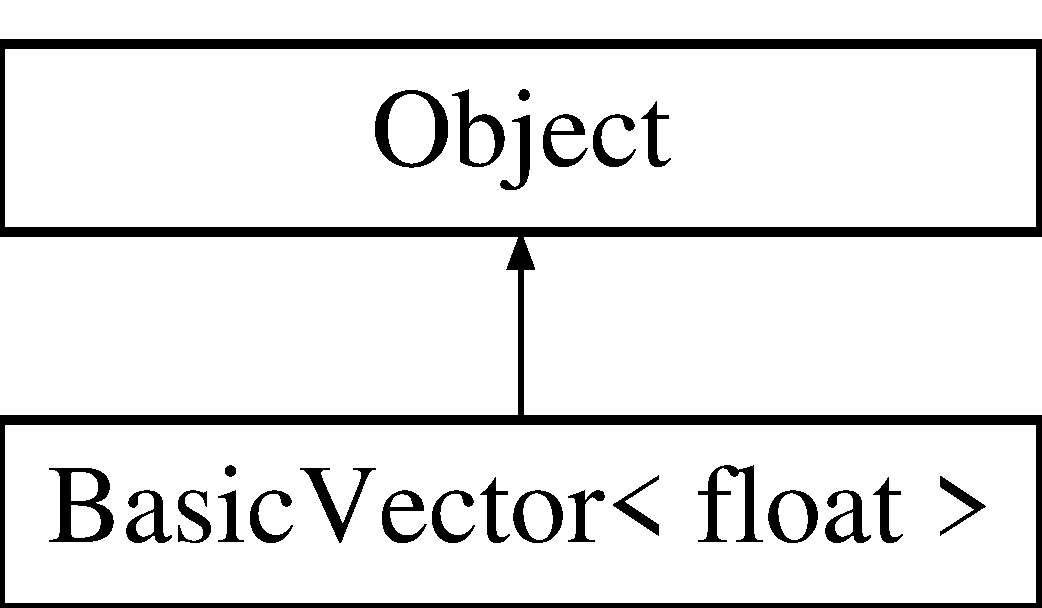
\includegraphics[height=2.000000cm]{classBasicVector_3_01float_01_4}
\end{center}
\end{figure}
\subsection*{Public Member Functions}
\begin{DoxyCompactItemize}
\item 
\hypertarget{classBasicVector_3_01float_01_4_ae309744da3e13579d30f8df6f9b7c9ed}{}\label{classBasicVector_3_01float_01_4_ae309744da3e13579d30f8df6f9b7c9ed} 
I\+N\+L\+I\+NE \hyperlink{classBasicVector_3_01float_01_4_ae309744da3e13579d30f8df6f9b7c9ed}{Basic\+Vector} (const \+\_\+\+\_\+m128 data)
\begin{DoxyCompactList}\small\item\em Constructs from S\+SE vector. \end{DoxyCompactList}\item 
\hypertarget{classBasicVector_3_01float_01_4_a781592c27e7c0921ccc39d2d9000ab36}{}\label{classBasicVector_3_01float_01_4_a781592c27e7c0921ccc39d2d9000ab36} 
I\+N\+L\+I\+NE \hyperlink{classBasicVector_3_01float_01_4_a781592c27e7c0921ccc39d2d9000ab36}{Basic\+Vector} (const float f)
\begin{DoxyCompactList}\small\item\em Constructs by copying a value to all vector components. \end{DoxyCompactList}\item 
\hypertarget{classBasicVector_3_01float_01_4_ad8445726393e01de743256cadb58c11f}{}\label{classBasicVector_3_01float_01_4_ad8445726393e01de743256cadb58c11f} 
I\+N\+L\+I\+NE \hyperlink{classBasicVector_3_01float_01_4_ad8445726393e01de743256cadb58c11f}{Basic\+Vector} (const float x, const float y, const float z=0.f, const float h=0.f)
\begin{DoxyCompactList}\small\item\em Constructs the vector from given components. \end{DoxyCompactList}\item 
\hypertarget{classBasicVector_3_01float_01_4_aa257e64fdb7ab1803bc19b7907f18f77}{}\label{classBasicVector_3_01float_01_4_aa257e64fdb7ab1803bc19b7907f18f77} 
I\+N\+L\+I\+NE \hyperlink{classBasicVector_3_01float_01_4_aa257e64fdb7ab1803bc19b7907f18f77}{Basic\+Vector} (const \hyperlink{classBasicVector}{Basic\+Vector} \&v)
\begin{DoxyCompactList}\small\item\em Copy constructor. \end{DoxyCompactList}\item 
\hypertarget{classBasicVector_3_01float_01_4_a0266fc91fed60b9720195065fe8686ee}{}\label{classBasicVector_3_01float_01_4_a0266fc91fed60b9720195065fe8686ee} 
I\+N\+L\+I\+NE \hyperlink{classBasicVector_3_01float_01_4_a0266fc91fed60b9720195065fe8686ee}{Basic\+Vector} (\hyperlink{classBasicVector}{Basic\+Vector} \&\&v)
\begin{DoxyCompactList}\small\item\em Move constructor. \end{DoxyCompactList}\item 
\hypertarget{classBasicVector_3_01float_01_4_a130beba5af7e15bc9d4584abf530a1fc}{}\label{classBasicVector_3_01float_01_4_a130beba5af7e15bc9d4584abf530a1fc} 
I\+N\+L\+I\+NE const float \& \hyperlink{classBasicVector_3_01float_01_4_a130beba5af7e15bc9d4584abf530a1fc}{operator\mbox{[}$\,$\mbox{]}} (const int i) const
\begin{DoxyCompactList}\small\item\em Get component by given index. \end{DoxyCompactList}\item 
\hypertarget{classBasicVector_3_01float_01_4_a60aa0ab99c1acf3382727e250e0517c9}{}\label{classBasicVector_3_01float_01_4_a60aa0ab99c1acf3382727e250e0517c9} 
I\+N\+L\+I\+NE float \& \hyperlink{classBasicVector_3_01float_01_4_a60aa0ab99c1acf3382727e250e0517c9}{operator\mbox{[}$\,$\mbox{]}} (const int i)
\begin{DoxyCompactList}\small\item\em Get component by given index. \end{DoxyCompactList}\item 
\hypertarget{classBasicVector_3_01float_01_4_a94d72134d2640242eaeda417d012f712}{}\label{classBasicVector_3_01float_01_4_a94d72134d2640242eaeda417d012f712} 
{\footnotesize template$<$int i$>$ }\\I\+N\+L\+I\+NE const float \& \hyperlink{classBasicVector_3_01float_01_4_a94d72134d2640242eaeda417d012f712}{get} () const
\begin{DoxyCompactList}\small\item\em Get component by given compile-\/time constant index. \end{DoxyCompactList}\item 
\hypertarget{classBasicVector_3_01float_01_4_ada76384c93d58c1fc7213da82f35f5e5}{}\label{classBasicVector_3_01float_01_4_ada76384c93d58c1fc7213da82f35f5e5} 
{\footnotesize template$<$int i$>$ }\\I\+N\+L\+I\+NE float \& \hyperlink{classBasicVector_3_01float_01_4_ada76384c93d58c1fc7213da82f35f5e5}{get} ()
\begin{DoxyCompactList}\small\item\em Get component by given compile-\/time constant index. \end{DoxyCompactList}\item 
\hypertarget{classBasicVector_3_01float_01_4_a60a7d21fa579a067d2aca9377b8c07c3}{}\label{classBasicVector_3_01float_01_4_a60a7d21fa579a067d2aca9377b8c07c3} 
I\+N\+L\+I\+NE \hyperlink{classBasicVector}{Basic\+Vector} \& \hyperlink{classBasicVector_3_01float_01_4_a60a7d21fa579a067d2aca9377b8c07c3}{operator=} (const \hyperlink{classBasicVector}{Basic\+Vector} \&v)
\begin{DoxyCompactList}\small\item\em Copy operator. \end{DoxyCompactList}\item 
\hypertarget{classBasicVector_3_01float_01_4_a53d2c286bfe02301a32d8364a090f861}{}\label{classBasicVector_3_01float_01_4_a53d2c286bfe02301a32d8364a090f861} 
I\+N\+L\+I\+NE \hyperlink{classBasicVector}{Basic\+Vector} \& \hyperlink{classBasicVector_3_01float_01_4_a53d2c286bfe02301a32d8364a090f861}{operator=} (\hyperlink{classBasicVector}{Basic\+Vector} \&\&v)
\begin{DoxyCompactList}\small\item\em Move operator. \end{DoxyCompactList}\item 
\hypertarget{classBasicVector_3_01float_01_4_a57a068befb024540766f31f74a5c18d3}{}\label{classBasicVector_3_01float_01_4_a57a068befb024540766f31f74a5c18d3} 
I\+N\+L\+I\+NE \hyperlink{classBasicVector}{Basic\+Vector} \& {\bfseries operator+=} (const \hyperlink{classBasicVector}{Basic\+Vector} \&v)
\item 
\hypertarget{classBasicVector_3_01float_01_4_a5dfe3be76ccc8f666d96121c75caa0f6}{}\label{classBasicVector_3_01float_01_4_a5dfe3be76ccc8f666d96121c75caa0f6} 
I\+N\+L\+I\+NE \hyperlink{classBasicVector}{Basic\+Vector} \& {\bfseries operator-\/=} (const \hyperlink{classBasicVector}{Basic\+Vector} \&v)
\item 
\hypertarget{classBasicVector_3_01float_01_4_a0581e62694aebe87bdc6ccc99d1976ac}{}\label{classBasicVector_3_01float_01_4_a0581e62694aebe87bdc6ccc99d1976ac} 
I\+N\+L\+I\+NE \hyperlink{classBasicVector}{Basic\+Vector} \& {\bfseries operator$\ast$=} (const float f)
\item 
\hypertarget{classBasicVector_3_01float_01_4_a4c10c0036349affc4e7633c9df85382d}{}\label{classBasicVector_3_01float_01_4_a4c10c0036349affc4e7633c9df85382d} 
I\+N\+L\+I\+NE \hyperlink{classBasicVector}{Basic\+Vector} \& {\bfseries operator/=} (const float f)
\item 
\hypertarget{classBasicVector_3_01float_01_4_a19b981b2e1e7db3acc31b1a2971087c5}{}\label{classBasicVector_3_01float_01_4_a19b981b2e1e7db3acc31b1a2971087c5} 
I\+N\+L\+I\+NE \hyperlink{classBasicVector}{Basic\+Vector} \& {\bfseries operator$\ast$=} (const \hyperlink{classBasicVector}{Basic\+Vector} \&v)
\item 
\hypertarget{classBasicVector_3_01float_01_4_a89678f5a80e7bba6ecadbcb7eccfef35}{}\label{classBasicVector_3_01float_01_4_a89678f5a80e7bba6ecadbcb7eccfef35} 
I\+N\+L\+I\+NE \hyperlink{classBasicVector}{Basic\+Vector} \& {\bfseries operator/=} (const \hyperlink{classBasicVector}{Basic\+Vector} \&v)
\item 
\hypertarget{classBasicVector_3_01float_01_4_ae534dab53da58849d72014e28ee35cc8}{}\label{classBasicVector_3_01float_01_4_ae534dab53da58849d72014e28ee35cc8} 
I\+N\+L\+I\+NE auto {\bfseries dot} (const \hyperlink{classBasicVector}{Basic\+Vector} \&other) const
\item 
\hypertarget{classBasicVector_3_01float_01_4_a6aef6aadecda8d1ba44c01a25e8a1e1d}{}\label{classBasicVector_3_01float_01_4_a6aef6aadecda8d1ba44c01a25e8a1e1d} 
I\+N\+L\+I\+NE auto {\bfseries cross} (const \hyperlink{classBasicVector}{Basic\+Vector} \&other) const
\item 
\hypertarget{classBasicVector_3_01float_01_4_a9aa5a6b8d3973b1054b9ca1dcc0de3fb}{}\label{classBasicVector_3_01float_01_4_a9aa5a6b8d3973b1054b9ca1dcc0de3fb} 
I\+N\+L\+I\+NE \hyperlink{classBasicVector}{Basic\+Vector} {\bfseries min} (const \hyperlink{classBasicVector}{Basic\+Vector} \&other) const
\item 
\hypertarget{classBasicVector_3_01float_01_4_ae50b9ac8eecaaa2727cf12a8c3885034}{}\label{classBasicVector_3_01float_01_4_ae50b9ac8eecaaa2727cf12a8c3885034} 
I\+N\+L\+I\+NE \hyperlink{classBasicVector}{Basic\+Vector} {\bfseries max} (const \hyperlink{classBasicVector}{Basic\+Vector} \&other) const
\end{DoxyCompactItemize}
\subsection*{Friends}
\begin{DoxyCompactItemize}
\item 
\hypertarget{classBasicVector_3_01float_01_4_a1f307378bb3c5832f697c8932d79848c}{}\label{classBasicVector_3_01float_01_4_a1f307378bb3c5832f697c8932d79848c} 
I\+N\+L\+I\+NE friend \hyperlink{classBasicVector}{Basic\+Vector} {\bfseries operator-\/} (const \hyperlink{classBasicVector}{Basic\+Vector} \&v)
\item 
\hypertarget{classBasicVector_3_01float_01_4_a52a8854619f1dbb9760107773b8631fe}{}\label{classBasicVector_3_01float_01_4_a52a8854619f1dbb9760107773b8631fe} 
I\+N\+L\+I\+NE friend \hyperlink{classBasicVector}{Basic\+Vector} {\bfseries operator+} (const \hyperlink{classBasicVector}{Basic\+Vector} \&v1, const \hyperlink{classBasicVector}{Basic\+Vector} \&v2)
\item 
\hypertarget{classBasicVector_3_01float_01_4_a752028cbae3f96cf020d4e9673faaecd}{}\label{classBasicVector_3_01float_01_4_a752028cbae3f96cf020d4e9673faaecd} 
I\+N\+L\+I\+NE friend \hyperlink{classBasicVector}{Basic\+Vector} {\bfseries operator-\/} (const \hyperlink{classBasicVector}{Basic\+Vector} \&v1, const \hyperlink{classBasicVector}{Basic\+Vector} \&v2)
\item 
\hypertarget{classBasicVector_3_01float_01_4_a0a30a111c264cc115c7d6fa2ba1d7650}{}\label{classBasicVector_3_01float_01_4_a0a30a111c264cc115c7d6fa2ba1d7650} 
I\+N\+L\+I\+NE friend auto \hyperlink{classBasicVector_3_01float_01_4_a0a30a111c264cc115c7d6fa2ba1d7650}{operator$\ast$} (const \hyperlink{classBasicVector}{Basic\+Vector} \&v, const float f)
\begin{DoxyCompactList}\small\item\em Multiplication of vector by a value or unit. \end{DoxyCompactList}\item 
\hypertarget{classBasicVector_3_01float_01_4_a2f6192488cd5b16eafc78ca0d05d9e10}{}\label{classBasicVector_3_01float_01_4_a2f6192488cd5b16eafc78ca0d05d9e10} 
I\+N\+L\+I\+NE friend auto {\bfseries operator$\ast$} (const float f, const \hyperlink{classBasicVector}{Basic\+Vector} \&v)
\item 
\hypertarget{classBasicVector_3_01float_01_4_afec38b18caebad20ce14e3d89ac6a272}{}\label{classBasicVector_3_01float_01_4_afec38b18caebad20ce14e3d89ac6a272} 
I\+N\+L\+I\+NE friend auto {\bfseries operator$\ast$} (const \hyperlink{classBasicVector}{Basic\+Vector} \&v1, const \hyperlink{classBasicVector}{Basic\+Vector} \&v2)
\item 
\hypertarget{classBasicVector_3_01float_01_4_a75b021a97f5880d9a5edbebf7ecd6075}{}\label{classBasicVector_3_01float_01_4_a75b021a97f5880d9a5edbebf7ecd6075} 
I\+N\+L\+I\+NE friend auto {\bfseries operator/} (const \hyperlink{classBasicVector}{Basic\+Vector} \&v, const float f)
\item 
\hypertarget{classBasicVector_3_01float_01_4_aa1877a346e7aa1ea57737628a58589e7}{}\label{classBasicVector_3_01float_01_4_aa1877a346e7aa1ea57737628a58589e7} 
I\+N\+L\+I\+NE friend auto {\bfseries operator/} (const \hyperlink{classBasicVector}{Basic\+Vector} \&v1, const \hyperlink{classBasicVector}{Basic\+Vector} \&v2)
\item 
\hypertarget{classBasicVector_3_01float_01_4_a89893ab07524d683177877fc3f1a34d6}{}\label{classBasicVector_3_01float_01_4_a89893ab07524d683177877fc3f1a34d6} 
I\+N\+L\+I\+NE friend bool \hyperlink{classBasicVector_3_01float_01_4_a89893ab07524d683177877fc3f1a34d6}{operator==} (const \hyperlink{classBasicVector}{Basic\+Vector} \&v1, const \hyperlink{classBasicVector}{Basic\+Vector} \&v2)
\begin{DoxyCompactList}\small\item\em Comparison operator, only enabled for vectors of same type. \end{DoxyCompactList}\item 
\hypertarget{classBasicVector_3_01float_01_4_a214517caa81358c78e46ffea40acab05}{}\label{classBasicVector_3_01float_01_4_a214517caa81358c78e46ffea40acab05} 
I\+N\+L\+I\+NE friend bool {\bfseries operator!=} (const \hyperlink{classBasicVector}{Basic\+Vector} \&v1, const \hyperlink{classBasicVector}{Basic\+Vector} \&v2)
\item 
\hypertarget{classBasicVector_3_01float_01_4_a326bb814a09dab7d58edd595b3db3813}{}\label{classBasicVector_3_01float_01_4_a326bb814a09dab7d58edd595b3db3813} 
{\footnotesize template$<$typename T\+Stream $>$ }\\T\+Stream \& {\bfseries operator$<$$<$} (T\+Stream \&stream, const \hyperlink{classBasicVector}{Basic\+Vector} \&v)
\end{DoxyCompactItemize}


\subsection{Detailed Description}
\subsubsection*{template$<$$>$\newline
class Basic\+Vector$<$ float $>$}

3-\/dimensional vector, float precision 

The documentation for this class was generated from the following file\+:\begin{DoxyCompactItemize}
\item 
/home/pavel/projects/astro/sph2/src/geometry/vector.\+h\end{DoxyCompactItemize}

\hypertarget{classBlockDomain}{}\section{Block\+Domain Class Reference}
\label{classBlockDomain}\index{Block\+Domain@{Block\+Domain}}
Inheritance diagram for Block\+Domain\+:\begin{figure}[H]
\begin{center}
\leavevmode
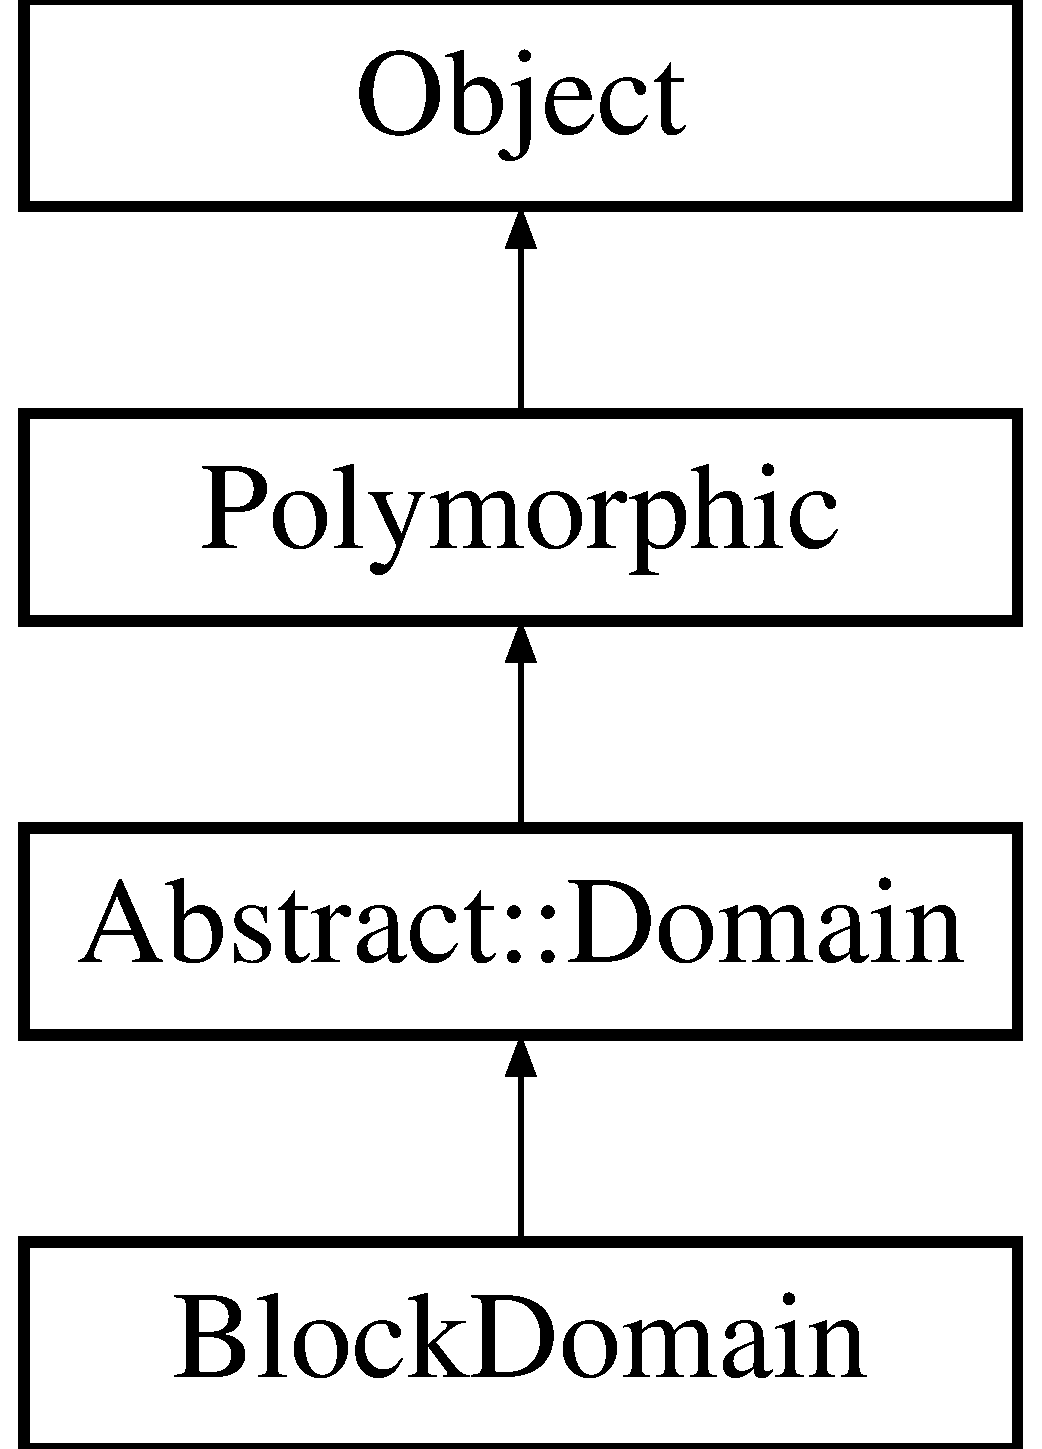
\includegraphics[height=4.000000cm]{classBlockDomain}
\end{center}
\end{figure}
\subsection*{Public Member Functions}
\begin{DoxyCompactItemize}
\item 
\hypertarget{classBlockDomain_af1564971dfe8aa95843fbc03bcccddb9}{}\label{classBlockDomain_af1564971dfe8aa95843fbc03bcccddb9} 
{\bfseries Block\+Domain} (const \hyperlink{classBasicVector}{Vector} \&center, const \hyperlink{classBasicVector}{Vector} \&edges)
\item 
\hypertarget{classBlockDomain_a02031b9f3dd6da6e2b1fca166b6ae6d4}{}\label{classBlockDomain_a02031b9f3dd6da6e2b1fca166b6ae6d4} 
virtual Float \hyperlink{classBlockDomain_a02031b9f3dd6da6e2b1fca166b6ae6d4}{get\+Volume} () const override
\begin{DoxyCompactList}\small\item\em Returns the total d-\/dimensional volume of the domain. \end{DoxyCompactList}\item 
\hypertarget{classBlockDomain_a4d191bf9138a19801cf1f2c5598563a0}{}\label{classBlockDomain_a4d191bf9138a19801cf1f2c5598563a0} 
virtual bool \hyperlink{classBlockDomain_a4d191bf9138a19801cf1f2c5598563a0}{is\+Inside} (const \hyperlink{classBasicVector}{Vector} \&v) const override
\begin{DoxyCompactList}\small\item\em Checks if the vector lies inside the domain. \end{DoxyCompactList}\item 
virtual void \hyperlink{classBlockDomain_a2dba56e9bbecdc5954147accfdcf331b}{are\+Inside} (const \hyperlink{classArrayView}{Array\+View}$<$ \hyperlink{classBasicVector}{Vector} $>$ vs, \hyperlink{classArrayView}{Array\+View}$<$ bool $>$ output) const override
\item 
\hypertarget{classBlockDomain_a7d9db768e866c04fb76ee3d81629974b}{}\label{classBlockDomain_a7d9db768e866c04fb76ee3d81629974b} 
virtual void \hyperlink{classBlockDomain_a7d9db768e866c04fb76ee3d81629974b}{project} (\hyperlink{classArrayView}{Array\+View}$<$ \hyperlink{classBasicVector}{Vector} $>$ vs) const override
\begin{DoxyCompactList}\small\item\em Projects vectors outside of the domain onto its boundary. Vectors inside the domains are untouched. \end{DoxyCompactList}\end{DoxyCompactItemize}
\subsection*{Additional Inherited Members}


\subsection{Member Function Documentation}
\hypertarget{classBlockDomain_a2dba56e9bbecdc5954147accfdcf331b}{}\label{classBlockDomain_a2dba56e9bbecdc5954147accfdcf331b} 
\index{Block\+Domain@{Block\+Domain}!are\+Inside@{are\+Inside}}
\index{are\+Inside@{are\+Inside}!Block\+Domain@{Block\+Domain}}
\subsubsection{\texorpdfstring{are\+Inside()}{areInside()}}
{\footnotesize\ttfamily virtual void Block\+Domain\+::are\+Inside (\begin{DoxyParamCaption}\item[{const \hyperlink{classArrayView}{Array\+View}$<$ \hyperlink{classBasicVector}{Vector} $>$}]{vs,  }\item[{\hyperlink{classArrayView}{Array\+View}$<$ bool $>$}]{output }\end{DoxyParamCaption}) const\hspace{0.3cm}{\ttfamily [inline]}, {\ttfamily [override]}, {\ttfamily [virtual]}}

Checks if elements of an array are inside the domain. Returns the result as array of bools. \hyperlink{classArray}{Array} must be already allocated and its size must match array vs. 

Implements \hyperlink{classAbstract_1_1Domain_a48ecb4ac3dab5f5a5e2de7b8e8218317}{Abstract\+::\+Domain}.



The documentation for this class was generated from the following file\+:\begin{DoxyCompactItemize}
\item 
/home/pavel/projects/astro/sph2/src/geometry/domain.\+h\end{DoxyCompactItemize}

\hypertarget{classBody}{}\section{Body Class Reference}
\label{classBody}\index{Body@{Body}}


{\ttfamily \#include $<$particle.\+h$>$}

Inheritance diagram for Body\+:\begin{figure}[H]
\begin{center}
\leavevmode
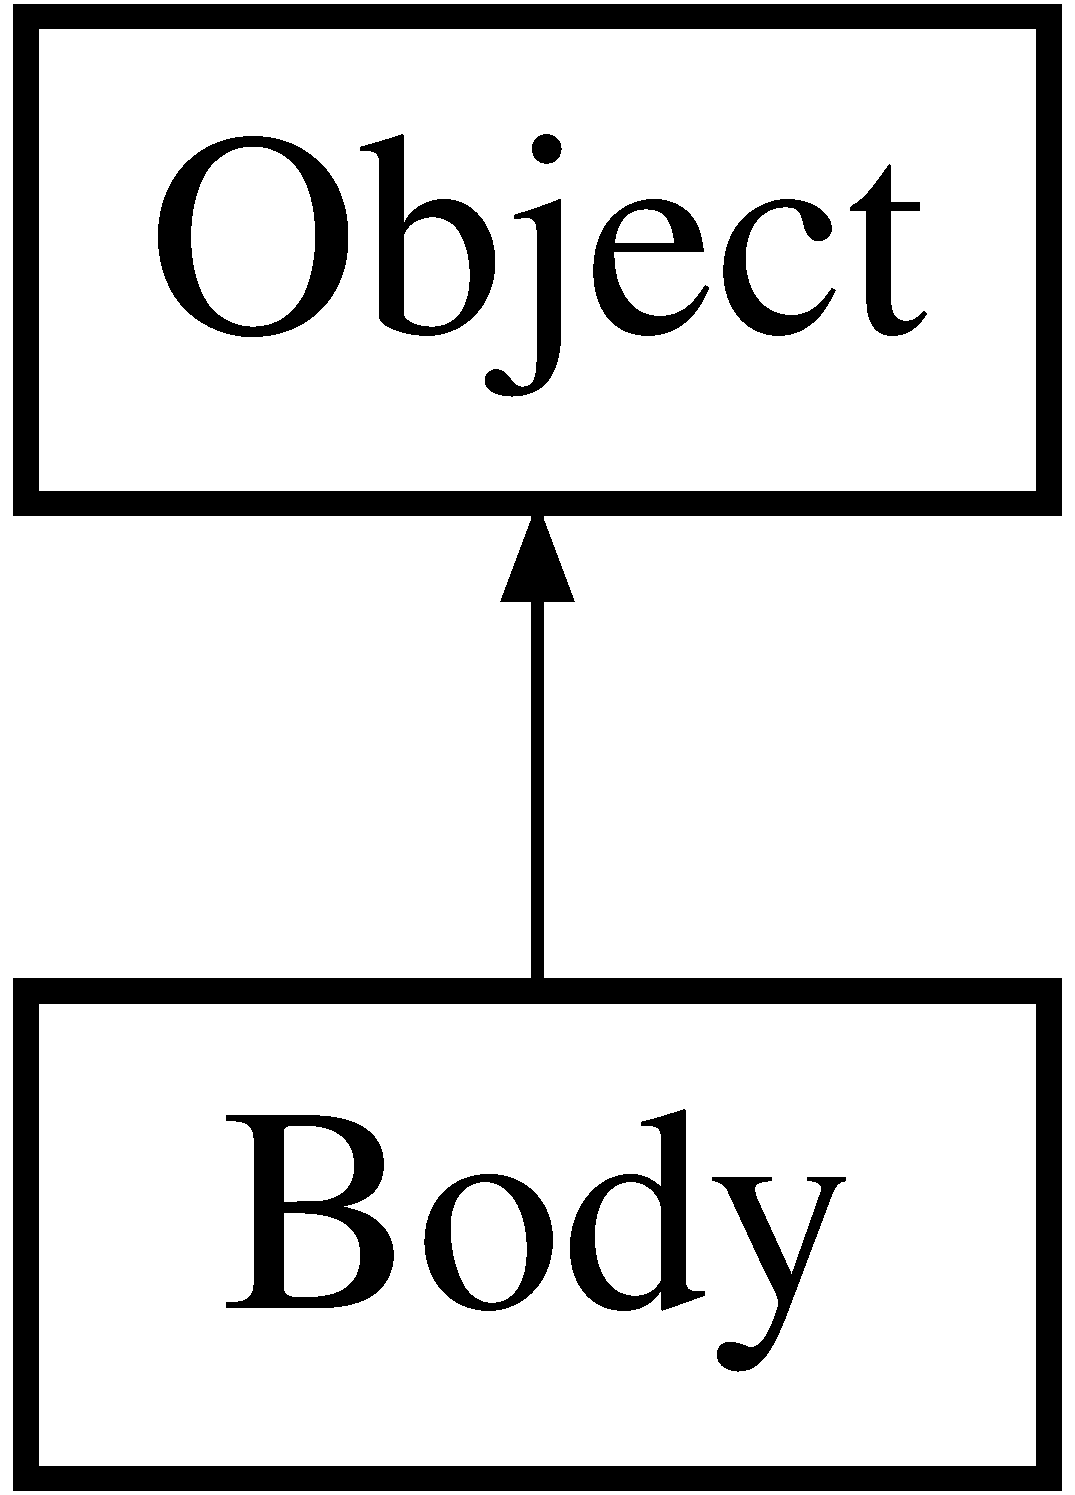
\includegraphics[height=2.000000cm]{classBody}
\end{center}
\end{figure}
\subsection*{Public Member Functions}
\begin{DoxyCompactItemize}
\item 
\hypertarget{classBody_a6e58829bd25233b0331c2e62b8d8934e}{}\label{classBody_a6e58829bd25233b0331c2e62b8d8934e} 
{\footnotesize template$<$Quantity\+Id ID$>$ }\\auto {\bfseries get} () const
\item 
\hypertarget{classBody_a345a4e3c96434dbb98740e78b2b2f615}{}\label{classBody_a345a4e3c96434dbb98740e78b2b2f615} 
void {\bfseries create} (const int n, const \hyperlink{classAbstract_1_1Domain}{Abstract\+::\+Domain} $\ast$domain, const \hyperlink{classAbstract_1_1Distribution}{Abstract\+::\+Distribution} $\ast$distribution, const \hyperlink{classSettings}{Settings}$<$ Body\+Settings\+Ids $>$ \&settings)
\item 
\hypertarget{classBody_acf614ab6b2734aa52bd8de02a0211ead}{}\label{classBody_acf614ab6b2734aa52bd8de02a0211ead} 
void \hyperlink{classBody_acf614ab6b2734aa52bd8de02a0211ead}{move} (const \hyperlink{classBasicVector}{Vector} \&offset)
\begin{DoxyCompactList}\small\item\em Moves all particles in given direction. Does not change velocities or other quantities. \end{DoxyCompactList}\item 
void \hyperlink{classBody_ad506a868ff9e989282cb948d44f35f42}{rotate} (const \hyperlink{classBasicVector}{Vector} \&U\+N\+U\+S\+ED(center), const \hyperlink{classBasicVector}{Vector} \&U\+N\+U\+S\+ED(axis))
\item 
\hypertarget{classBody_acd8c26a7a416b6c579ca7ca447552fd1}{}\label{classBody_acd8c26a7a416b6c579ca7ca447552fd1} 
void \hyperlink{classBody_acd8c26a7a416b6c579ca7ca447552fd1}{add\+Velocity} (const \hyperlink{classBasicVector}{Vector} \&velocity)
\begin{DoxyCompactList}\small\item\em Adds velocity to all particles. \end{DoxyCompactList}\item 
void \hyperlink{classBody_aefc7d09616d51ba1652a4a6940b06c5e}{add\+Angular\+Velocity} (const \hyperlink{classBasicVector}{Vector} \&U\+N\+U\+S\+ED(center), const \hyperlink{classBasicVector}{Vector} \&U\+N\+U\+S\+ED(axis))
\begin{DoxyCompactList}\small\item\em Adds angular velocity around given center and axis of rotation. \end{DoxyCompactList}\item 
\hypertarget{classBody_a39e2c28c977c5c6f1ab30b8790186eee}{}\label{classBody_a39e2c28c977c5c6f1ab30b8790186eee} 
void {\bfseries merge} (const \hyperlink{classBody}{Body} \&other)
\item 
\hypertarget{classBody_ade96d728b06622303593eef008a58591}{}\label{classBody_ade96d728b06622303593eef008a58591} 
void {\bfseries save\+To\+File} (const std\+::string \&path)
\end{DoxyCompactItemize}
\subsection*{Protected Attributes}
\begin{DoxyCompactItemize}
\item 
\hypertarget{classBody_a0f9839e3021bcd563d5b2eff97b96339}{}\label{classBody_a0f9839e3021bcd563d5b2eff97b96339} 
int \hyperlink{classBody_a0f9839e3021bcd563d5b2eff97b96339}{N}
\begin{DoxyCompactList}\small\item\em The number of particles. \end{DoxyCompactList}\item 
\hypertarget{classBody_aa1edcd0f5cc675e042fec4e494e52e48}{}\label{classBody_aa1edcd0f5cc675e042fec4e494e52e48} 
\hyperlink{classArray}{Array}$<$ \hyperlink{classBasicVector}{Vector} $>$ \hyperlink{classBody_aa1edcd0f5cc675e042fec4e494e52e48}{rs}
\begin{DoxyCompactList}\small\item\em Coordinates of particles, fourth component is smoothing length. \end{DoxyCompactList}\item 
\hypertarget{classBody_a08cf717fc912ebf9b792119c4b3808fd}{}\label{classBody_a08cf717fc912ebf9b792119c4b3808fd} 
\hyperlink{classArray}{Array}$<$ \hyperlink{classBasicVector}{Vector} $>$ \hyperlink{classBody_a08cf717fc912ebf9b792119c4b3808fd}{vs}
\begin{DoxyCompactList}\small\item\em Velocities of particles, fourth component if velocity divergence. \end{DoxyCompactList}\item 
\hypertarget{classBody_afc78fa820ba77712a298dcd1cab36254}{}\label{classBody_afc78fa820ba77712a298dcd1cab36254} 
\hyperlink{classArray}{Array}$<$ \hyperlink{classBasicVector}{Vector} $>$ \hyperlink{classBody_afc78fa820ba77712a298dcd1cab36254}{dvs}
\begin{DoxyCompactList}\small\item\em Acceleration. \end{DoxyCompactList}\item 
\hypertarget{classBody_a64fe5671c857851d4a21225e68291cd2}{}\label{classBody_a64fe5671c857851d4a21225e68291cd2} 
\hyperlink{classArray}{Array}$<$ Float $>$ \hyperlink{classBody_a64fe5671c857851d4a21225e68291cd2}{ms}
\begin{DoxyCompactList}\small\item\em Mass of S\+PH particles. \end{DoxyCompactList}\item 
\hypertarget{classBody_af575f15071511dfb25bcc6e653b2c605}{}\label{classBody_af575f15071511dfb25bcc6e653b2c605} 
\hyperlink{classArray}{Array}$<$ Float $>$ \hyperlink{classBody_af575f15071511dfb25bcc6e653b2c605}{rhos}
\begin{DoxyCompactList}\small\item\em Density. \end{DoxyCompactList}\item 
\hypertarget{classBody_ad97a2b2ca09bd5f099c5b5a398f5a7e1}{}\label{classBody_ad97a2b2ca09bd5f099c5b5a398f5a7e1} 
\hyperlink{classArray}{Array}$<$ Float $>$ \hyperlink{classBody_ad97a2b2ca09bd5f099c5b5a398f5a7e1}{drhos}
\begin{DoxyCompactList}\small\item\em Density derivative. \end{DoxyCompactList}\item 
\hypertarget{classBody_ae5ed29defd3c45d482a93d18590fc66d}{}\label{classBody_ae5ed29defd3c45d482a93d18590fc66d} 
\hyperlink{classArray}{Array}$<$ Float $>$ \hyperlink{classBody_ae5ed29defd3c45d482a93d18590fc66d}{ps}
\begin{DoxyCompactList}\small\item\em Pressure. \end{DoxyCompactList}\item 
\hypertarget{classBody_a49b491639fae94f1dfcdc84845af2c6b}{}\label{classBody_a49b491639fae94f1dfcdc84845af2c6b} 
\hyperlink{classArray}{Array}$<$ Float $>$ \hyperlink{classBody_a49b491639fae94f1dfcdc84845af2c6b}{us}
\begin{DoxyCompactList}\small\item\em Specific internal energy (=energy per unit mass) \end{DoxyCompactList}\item 
\hypertarget{classBody_a60bbb48380ae9e8a8dea2e7a88a5bf27}{}\label{classBody_a60bbb48380ae9e8a8dea2e7a88a5bf27} 
\hyperlink{classArray}{Array}$<$ Float $>$ \hyperlink{classBody_a60bbb48380ae9e8a8dea2e7a88a5bf27}{dus}
\begin{DoxyCompactList}\small\item\em Derivative of internal energy;. \end{DoxyCompactList}\end{DoxyCompactItemize}


\subsection{Detailed Description}
Base class storing arrays of particle quantities. If a model requires more quantities, it must inherits from this method and extend interface. 

\subsection{Member Function Documentation}
\hypertarget{classBody_aefc7d09616d51ba1652a4a6940b06c5e}{}\label{classBody_aefc7d09616d51ba1652a4a6940b06c5e} 
\index{Body@{Body}!add\+Angular\+Velocity@{add\+Angular\+Velocity}}
\index{add\+Angular\+Velocity@{add\+Angular\+Velocity}!Body@{Body}}
\subsubsection{\texorpdfstring{add\+Angular\+Velocity()}{addAngularVelocity()}}
{\footnotesize\ttfamily void Body\+::add\+Angular\+Velocity (\begin{DoxyParamCaption}\item[{const \hyperlink{classBasicVector}{Vector} \&}]{U\+N\+U\+S\+EDcenter,  }\item[{const \hyperlink{classBasicVector}{Vector} \&}]{U\+N\+U\+S\+EDaxis }\end{DoxyParamCaption})\hspace{0.3cm}{\ttfamily [inline]}}



Adds angular velocity around given center and axis of rotation. 

\begin{DoxyRefDesc}{Todo}
\item[\hyperlink{todo__todo000006}{Todo}]\end{DoxyRefDesc}
\hypertarget{classBody_ad506a868ff9e989282cb948d44f35f42}{}\label{classBody_ad506a868ff9e989282cb948d44f35f42} 
\index{Body@{Body}!rotate@{rotate}}
\index{rotate@{rotate}!Body@{Body}}
\subsubsection{\texorpdfstring{rotate()}{rotate()}}
{\footnotesize\ttfamily void Body\+::rotate (\begin{DoxyParamCaption}\item[{const \hyperlink{classBasicVector}{Vector} \&}]{U\+N\+U\+S\+EDcenter,  }\item[{const \hyperlink{classBasicVector}{Vector} \&}]{U\+N\+U\+S\+EDaxis }\end{DoxyParamCaption})\hspace{0.3cm}{\ttfamily [inline]}}

\begin{DoxyRefDesc}{Todo}
\item[\hyperlink{todo__todo000005}{Todo}]\end{DoxyRefDesc}


The documentation for this class was generated from the following file\+:\begin{DoxyCompactItemize}
\item 
/home/pavel/projects/astro/sph2/src/core/particle.\+h\end{DoxyCompactItemize}

\hypertarget{classBoundingBox}{}\section{Bounding\+Box$<$ T, d $>$ Class Template Reference}
\label{classBoundingBox}\index{Bounding\+Box$<$ T, d $>$@{Bounding\+Box$<$ T, d $>$}}
\subsection*{Public Member Functions}
\begin{DoxyCompactItemize}
\item 
\hypertarget{classBoundingBox_a918f0921f2ce317b1297db352292d4cd}{}\label{classBoundingBox_a918f0921f2ce317b1297db352292d4cd} 
void {\bfseries extend} (const \hyperlink{classBasicVector}{Vector}$<$ T, d $>$ \&v)
\item 
\hypertarget{classBoundingBox_a984f46b3ad79777f4051153e5549ee95}{}\label{classBoundingBox_a984f46b3ad79777f4051153e5549ee95} 
\hyperlink{classBasicVector}{Vector}$<$ T, d $>$ {\bfseries get\+Center} () const
\item 
\hypertarget{classBoundingBox_ada34d9a68df6943dba6704f9c49f4204}{}\label{classBoundingBox_ada34d9a68df6943dba6704f9c49f4204} 
\hyperlink{classBasicVector}{Vector}$<$ T, d $>$ {\bfseries get\+Dimensions} () const
\item 
\hypertarget{classBoundingBox_adab07a904560034560b6c4b0d870338e}{}\label{classBoundingBox_adab07a904560034560b6c4b0d870338e} 
T {\bfseries get\+Volume} () const
\item 
\hypertarget{classBoundingBox_a9d99863e7febbee132cab18948be42e7}{}\label{classBoundingBox_a9d99863e7febbee132cab18948be42e7} 
bool {\bfseries is\+Inside} (const \hyperlink{classBasicVector}{Vector}$<$ T, d $>$ \&v)
\end{DoxyCompactItemize}


The documentation for this class was generated from the following file\+:\begin{DoxyCompactItemize}
\item 
/home/pavel/projects/astro/sph2/src/tree/octree.\+h\end{DoxyCompactItemize}

\hypertarget{classBox}{}\section{Box Class Reference}
\label{classBox}\index{Box@{Box}}
Inheritance diagram for Box\+:\begin{figure}[H]
\begin{center}
\leavevmode
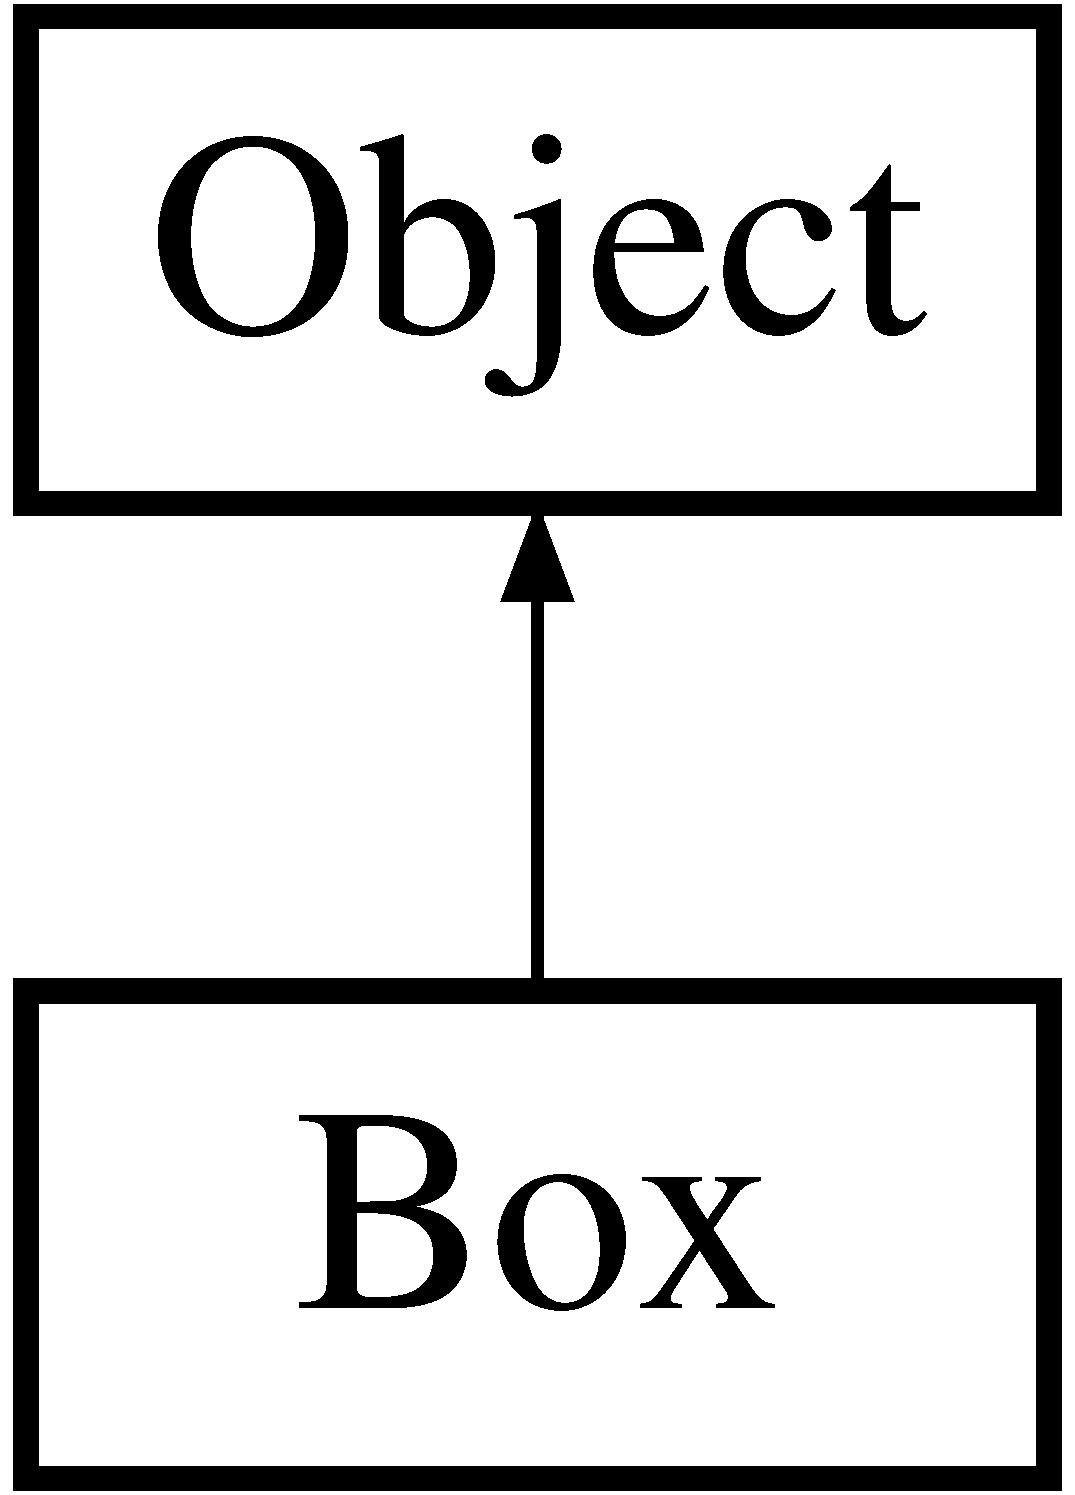
\includegraphics[height=2.000000cm]{classBox}
\end{center}
\end{figure}
\subsection*{Public Member Functions}
\begin{DoxyCompactItemize}
\item 
\hypertarget{classBox_a8c328c18411cc1ade2b95f41e157e9a7}{}\label{classBox_a8c328c18411cc1ade2b95f41e157e9a7} 
{\bfseries Box} (const \hyperlink{classBasicVector}{Vector} \&min\+Bound, const \hyperlink{classBasicVector}{Vector} \&max\+Bound)
\item 
\hypertarget{classBox_aad914d290bee7d61a8bb9e3ac6a3a0c4}{}\label{classBox_aad914d290bee7d61a8bb9e3ac6a3a0c4} 
void \hyperlink{classBox_aad914d290bee7d61a8bb9e3ac6a3a0c4}{extend} (const \hyperlink{classBasicVector}{Vector} \&v)
\begin{DoxyCompactList}\small\item\em Enlarges the box to contain the vector;. \end{DoxyCompactList}\item 
\hypertarget{classBox_ab63d1b877eac090299b2e7f1966e4e6e}{}\label{classBox_ab63d1b877eac090299b2e7f1966e4e6e} 
bool \hyperlink{classBox_ab63d1b877eac090299b2e7f1966e4e6e}{contains} (const \hyperlink{classBasicVector}{Vector} \&v) const
\begin{DoxyCompactList}\small\item\em Checks if the vector lies inside the box. \end{DoxyCompactList}\item 
\hypertarget{classBox_adf1d609338da84d31c8b0e010fe5f907}{}\label{classBox_adf1d609338da84d31c8b0e010fe5f907} 
\hyperlink{classBasicVector}{Vector} \hyperlink{classBox_adf1d609338da84d31c8b0e010fe5f907}{clamp} (const \hyperlink{classBasicVector}{Vector} \&v) const
\begin{DoxyCompactList}\small\item\em Clamps all components of the vector to fit within the box. \end{DoxyCompactList}\item 
\hypertarget{classBox_a31dcc6067218190c5cb781b8798ff23d}{}\label{classBox_a31dcc6067218190c5cb781b8798ff23d} 
I\+N\+L\+I\+NE const \hyperlink{classBasicVector}{Vector} \& {\bfseries lower} () const
\item 
\hypertarget{classBox_a605768bd1e2d0cd6bf00c55414501d78}{}\label{classBox_a605768bd1e2d0cd6bf00c55414501d78} 
I\+N\+L\+I\+NE \hyperlink{classBasicVector}{Vector} \& {\bfseries lower} ()
\item 
\hypertarget{classBox_a5065b3a87925aa52ff527da479284f9a}{}\label{classBox_a5065b3a87925aa52ff527da479284f9a} 
I\+N\+L\+I\+NE const \hyperlink{classBasicVector}{Vector} \& {\bfseries upper} () const
\item 
\hypertarget{classBox_aaee9e6a44373409fef03e2a2e0284d6c}{}\label{classBox_aaee9e6a44373409fef03e2a2e0284d6c} 
I\+N\+L\+I\+NE \hyperlink{classBasicVector}{Vector} \& {\bfseries upper} ()
\item 
\hypertarget{classBox_aaef966bd93d65ff36f608e9607399c46}{}\label{classBox_aaef966bd93d65ff36f608e9607399c46} 
I\+N\+L\+I\+NE \hyperlink{classBasicVector}{Vector} {\bfseries get\+Size} () const
\item 
\hypertarget{classBox_ab251a2559bbb4e6af3caddcc9aea5e1f}{}\label{classBox_ab251a2559bbb4e6af3caddcc9aea5e1f} 
Float {\bfseries get\+Volume} () const
\item 
\hypertarget{classBox_ad2e05c5df3f534141e6f7516ab17e835}{}\label{classBox_ad2e05c5df3f534141e6f7516ab17e835} 
{\footnotesize template$<$typename T\+Functor $>$ }\\void \hyperlink{classBox_ad2e05c5df3f534141e6f7516ab17e835}{iterate} (const \hyperlink{classBasicVector}{Vector} \&step, T\+Functor \&\&functor) const
\begin{DoxyCompactList}\small\item\em Execute functor for all possible values of vector (with constant stepping) \end{DoxyCompactList}\item 
{\footnotesize template$<$typename T\+Functor $>$ }\\void \hyperlink{classBox_a6802c8d00894fe5a3098e5a3d7d2184b}{iterate\+With\+Indices} (const \hyperlink{classBasicVector}{Vector} \&step, T\+Functor \&\&functor) const
\end{DoxyCompactItemize}


\subsection{Member Function Documentation}
\hypertarget{classBox_a6802c8d00894fe5a3098e5a3d7d2184b}{}\label{classBox_a6802c8d00894fe5a3098e5a3d7d2184b} 
\index{Box@{Box}!iterate\+With\+Indices@{iterate\+With\+Indices}}
\index{iterate\+With\+Indices@{iterate\+With\+Indices}!Box@{Box}}
\subsubsection{\texorpdfstring{iterate\+With\+Indices()}{iterateWithIndices()}}
{\footnotesize\ttfamily template$<$typename T\+Functor $>$ \\
void Box\+::iterate\+With\+Indices (\begin{DoxyParamCaption}\item[{const \hyperlink{classBasicVector}{Vector} \&}]{step,  }\item[{T\+Functor \&\&}]{functor }\end{DoxyParamCaption}) const\hspace{0.3cm}{\ttfamily [inline]}}

Execute functor for all possible values of vector (with constant stepping), passing auxiliary indices together with the vector 

The documentation for this class was generated from the following file\+:\begin{DoxyCompactItemize}
\item 
/home/pavel/projects/astro/sph2/src/geometry/bounds.\+h\end{DoxyCompactItemize}

\hypertarget{classBruteForceFinder}{}\section{Brute\+Force\+Finder Class Reference}
\label{classBruteForceFinder}\index{Brute\+Force\+Finder@{Brute\+Force\+Finder}}


Search for neighbours by \textquotesingle{}brute force\textquotesingle{}, comparing every pair of vectors. Useful for testing other finders.  




{\ttfamily \#include $<$bruteforce.\+h$>$}

Inheritance diagram for Brute\+Force\+Finder\+:\begin{figure}[H]
\begin{center}
\leavevmode
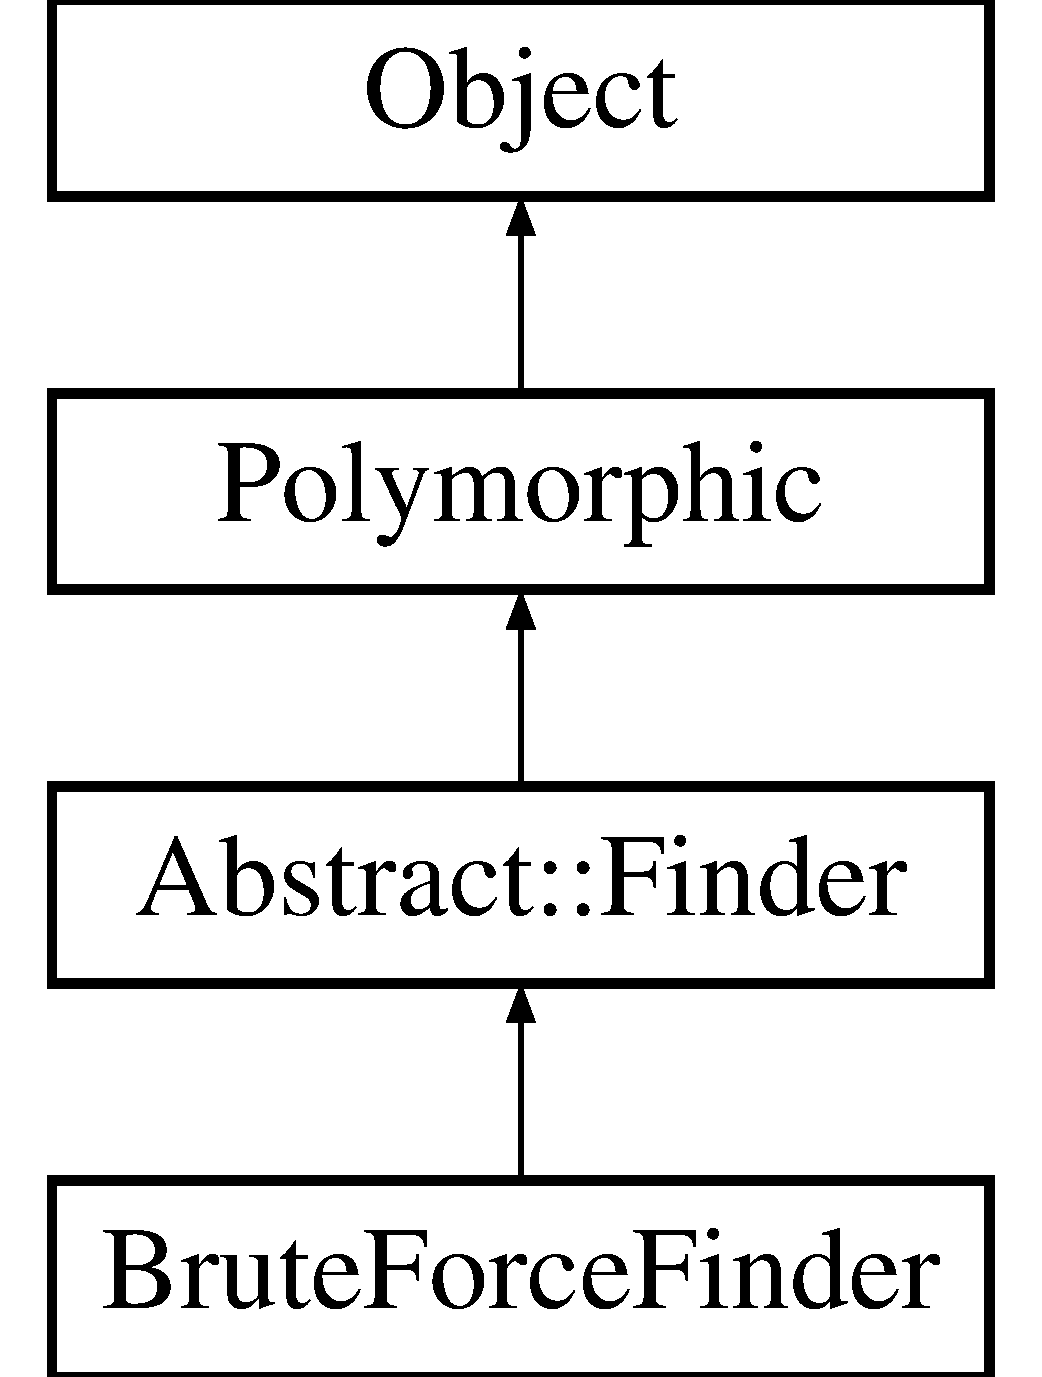
\includegraphics[height=4.000000cm]{classBruteForceFinder}
\end{center}
\end{figure}
\subsection*{Public Member Functions}
\begin{DoxyCompactItemize}
\item 
\hypertarget{classBruteForceFinder_a9cbffd174d9cc0997a0ab013f37c9fa3}{}\label{classBruteForceFinder_a9cbffd174d9cc0997a0ab013f37c9fa3} 
virtual int {\bfseries find\+Neighbours} (const int index, const Float radius, \hyperlink{classArray}{Array}$<$ \hyperlink{structNeighbourRecord}{Neighbour\+Record} $>$ \&neighbours, \hyperlink{classFlags}{Flags}$<$ Finder\+Flags $>$ flags=E\+M\+P\+T\+Y\+\_\+\+F\+L\+A\+GS, const Float U\+N\+U\+S\+ED(error)=0.\+\_\+f) const override
\item 
\hypertarget{classBruteForceFinder_a139b10deee1d18d4584f291b1c319eb7}{}\label{classBruteForceFinder_a139b10deee1d18d4584f291b1c319eb7} 
virtual void \hyperlink{classBruteForceFinder_a139b10deee1d18d4584f291b1c319eb7}{rebuild} ()
\begin{DoxyCompactList}\small\item\em Updates the structure when the position change. \end{DoxyCompactList}\end{DoxyCompactItemize}
\subsection*{Protected Member Functions}
\begin{DoxyCompactItemize}
\item 
\hypertarget{classBruteForceFinder_a5fa881f7d87ae23d10759c873855448f}{}\label{classBruteForceFinder_a5fa881f7d87ae23d10759c873855448f} 
virtual void {\bfseries build\+Impl} (\hyperlink{classArrayView}{Array\+View}$<$ \hyperlink{classBasicVector}{Vector} $>$ U\+N\+U\+S\+ED(values)) override
\end{DoxyCompactItemize}
\subsection*{Additional Inherited Members}


\subsection{Detailed Description}
Search for neighbours by \textquotesingle{}brute force\textquotesingle{}, comparing every pair of vectors. Useful for testing other finders. 

The documentation for this class was generated from the following file\+:\begin{DoxyCompactItemize}
\item 
/home/pavel/projects/astro/sph2/src/tree/bruteforce.\+h\end{DoxyCompactItemize}

\hypertarget{classAbstract_1_1Callbacks}{}\section{Abstract\+:\+:Callbacks Class Reference}
\label{classAbstract_1_1Callbacks}\index{Abstract\+::\+Callbacks@{Abstract\+::\+Callbacks}}
Inheritance diagram for Abstract\+:\+:Callbacks\+:\begin{figure}[H]
\begin{center}
\leavevmode
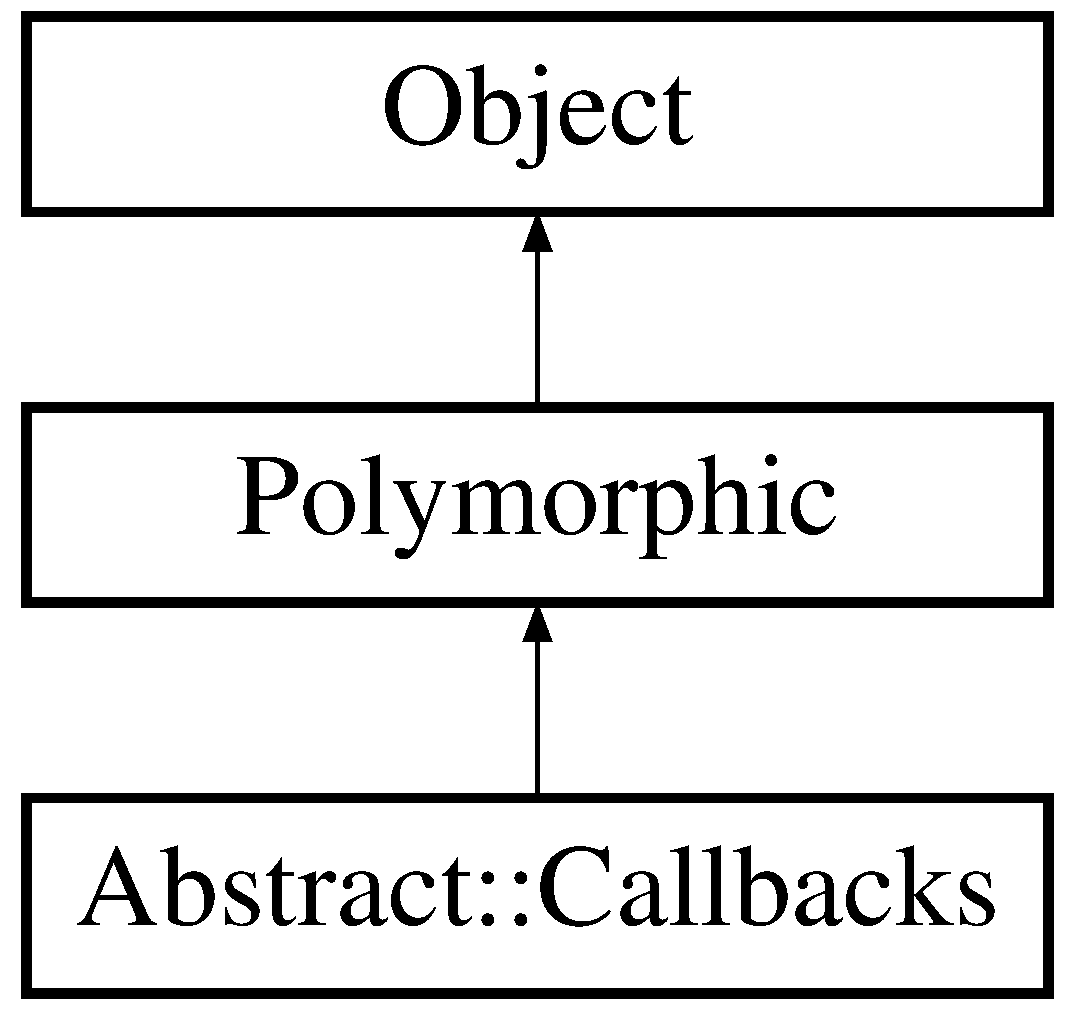
\includegraphics[height=3.000000cm]{classAbstract_1_1Callbacks}
\end{center}
\end{figure}
\subsection*{Public Member Functions}
\begin{DoxyCompactItemize}
\item 
\hypertarget{classAbstract_1_1Callbacks_a3e98ef18d54fb6f8a08df71f2d13cb9c}{}\label{classAbstract_1_1Callbacks_a3e98ef18d54fb6f8a08df71f2d13cb9c} 
virtual void {\bfseries on\+Time\+Step} (\hyperlink{classArrayView}{Array\+View}$<$ const \hyperlink{classBasicVector}{Vector} $>$ positions)=0
\end{DoxyCompactItemize}


The documentation for this class was generated from the following file\+:\begin{DoxyCompactItemize}
\item 
/home/pavel/projects/astro/sph2/src/system/callbacks.\+h\end{DoxyCompactItemize}

\hypertarget{classSph_1_1CArray}{}\section{Sph\+:\+:C\+Array$<$ T, N $>$ Class Template Reference}
\label{classSph_1_1CArray}\index{Sph\+::\+C\+Array$<$ T, N $>$@{Sph\+::\+C\+Array$<$ T, N $>$}}


{\ttfamily \#include $<$nanoflann.\+h$>$}

\subsection*{Public Types}
\begin{DoxyCompactItemize}
\item 
\hypertarget{classSph_1_1CArray_a7cd672d88f876ea0335c45b05596f94d}{}\label{classSph_1_1CArray_a7cd672d88f876ea0335c45b05596f94d} 
enum \{ {\bfseries static\+\_\+size} = N
 \}
\item 
\hypertarget{classSph_1_1CArray_ab5e5d57a00b35bef4acdbb65c2f58053}{}\label{classSph_1_1CArray_ab5e5d57a00b35bef4acdbb65c2f58053} 
typedef T {\bfseries value\+\_\+type}
\item 
\hypertarget{classSph_1_1CArray_a5ab5043e9807a80c3231a5095990afb9}{}\label{classSph_1_1CArray_a5ab5043e9807a80c3231a5095990afb9} 
typedef T $\ast$ {\bfseries iterator}
\item 
\hypertarget{classSph_1_1CArray_a605108f93a356bea2ad4d1b4965db468}{}\label{classSph_1_1CArray_a605108f93a356bea2ad4d1b4965db468} 
typedef const T $\ast$ {\bfseries const\+\_\+iterator}
\item 
\hypertarget{classSph_1_1CArray_aa9618701c693d2cfc93037f6845693d7}{}\label{classSph_1_1CArray_aa9618701c693d2cfc93037f6845693d7} 
typedef T \& {\bfseries reference}
\item 
\hypertarget{classSph_1_1CArray_ae2a21c36aa741ba6386da42ce2c97da9}{}\label{classSph_1_1CArray_ae2a21c36aa741ba6386da42ce2c97da9} 
typedef const T \& {\bfseries const\+\_\+reference}
\item 
\hypertarget{classSph_1_1CArray_ab46e7962656ad78df32565d71ca809b3}{}\label{classSph_1_1CArray_ab46e7962656ad78df32565d71ca809b3} 
typedef std\+::size\+\_\+t {\bfseries size\+\_\+type}
\item 
\hypertarget{classSph_1_1CArray_aa6d393f289c446e0be8bca1c4109cdd9}{}\label{classSph_1_1CArray_aa6d393f289c446e0be8bca1c4109cdd9} 
typedef std\+::ptrdiff\+\_\+t {\bfseries difference\+\_\+type}
\item 
\hypertarget{classSph_1_1CArray_a6d98ea796c993f005dab935891c4b168}{}\label{classSph_1_1CArray_a6d98ea796c993f005dab935891c4b168} 
typedef std\+::reverse\+\_\+iterator$<$ iterator $>$ {\bfseries reverse\+\_\+iterator}
\item 
\hypertarget{classSph_1_1CArray_af224ccc17a49817f54ab8a272d385aa1}{}\label{classSph_1_1CArray_af224ccc17a49817f54ab8a272d385aa1} 
typedef std\+::reverse\+\_\+iterator$<$ const\+\_\+iterator $>$ {\bfseries const\+\_\+reverse\+\_\+iterator}
\end{DoxyCompactItemize}
\subsection*{Public Member Functions}
\begin{DoxyCompactItemize}
\item 
\hypertarget{classSph_1_1CArray_a0871596ee9bde35f4ec59c85dd48736e}{}\label{classSph_1_1CArray_a0871596ee9bde35f4ec59c85dd48736e} 
iterator {\bfseries begin} ()
\item 
\hypertarget{classSph_1_1CArray_a0ead928a520f60017b89380eaca562bb}{}\label{classSph_1_1CArray_a0ead928a520f60017b89380eaca562bb} 
const\+\_\+iterator {\bfseries begin} () const
\item 
\hypertarget{classSph_1_1CArray_a42741661c05c9227a2e490009081cf1b}{}\label{classSph_1_1CArray_a42741661c05c9227a2e490009081cf1b} 
iterator {\bfseries end} ()
\item 
\hypertarget{classSph_1_1CArray_af6ef1db88d86387e389c7335e5ecc1d2}{}\label{classSph_1_1CArray_af6ef1db88d86387e389c7335e5ecc1d2} 
const\+\_\+iterator {\bfseries end} () const
\item 
\hypertarget{classSph_1_1CArray_a73541a8afd667066bc8bf880caba1889}{}\label{classSph_1_1CArray_a73541a8afd667066bc8bf880caba1889} 
reverse\+\_\+iterator {\bfseries rbegin} ()
\item 
\hypertarget{classSph_1_1CArray_aaeebae2e11d397f8089aec75077326b0}{}\label{classSph_1_1CArray_aaeebae2e11d397f8089aec75077326b0} 
const\+\_\+reverse\+\_\+iterator {\bfseries rbegin} () const
\item 
\hypertarget{classSph_1_1CArray_a6d661c5ca64dd063b87986864dc718e1}{}\label{classSph_1_1CArray_a6d661c5ca64dd063b87986864dc718e1} 
reverse\+\_\+iterator {\bfseries rend} ()
\item 
\hypertarget{classSph_1_1CArray_a832b85926d62171376e190c1643eaf8c}{}\label{classSph_1_1CArray_a832b85926d62171376e190c1643eaf8c} 
const\+\_\+reverse\+\_\+iterator {\bfseries rend} () const
\item 
\hypertarget{classSph_1_1CArray_aa5d410bc82aa19c9f4c37f3fa7fbbbdf}{}\label{classSph_1_1CArray_aa5d410bc82aa19c9f4c37f3fa7fbbbdf} 
reference {\bfseries operator\mbox{[}$\,$\mbox{]}} (size\+\_\+type i)
\item 
\hypertarget{classSph_1_1CArray_a7b8dfa8f8ce890e71c568e45b6588c18}{}\label{classSph_1_1CArray_a7b8dfa8f8ce890e71c568e45b6588c18} 
const\+\_\+reference {\bfseries operator\mbox{[}$\,$\mbox{]}} (size\+\_\+type i) const
\item 
\hypertarget{classSph_1_1CArray_af118438a8046480173ea261e6c112aa3}{}\label{classSph_1_1CArray_af118438a8046480173ea261e6c112aa3} 
reference {\bfseries at} (size\+\_\+type i)
\item 
\hypertarget{classSph_1_1CArray_a9cb82eaa97aa23cbe864e6153aaae68d}{}\label{classSph_1_1CArray_a9cb82eaa97aa23cbe864e6153aaae68d} 
const\+\_\+reference {\bfseries at} (size\+\_\+type i) const
\item 
\hypertarget{classSph_1_1CArray_ae9f12154cbce9a16bb5769c2b49c14b1}{}\label{classSph_1_1CArray_ae9f12154cbce9a16bb5769c2b49c14b1} 
reference {\bfseries front} ()
\item 
\hypertarget{classSph_1_1CArray_aa4996fb41c9b9120bb37eb24fdce5f90}{}\label{classSph_1_1CArray_aa4996fb41c9b9120bb37eb24fdce5f90} 
const\+\_\+reference {\bfseries front} () const
\item 
\hypertarget{classSph_1_1CArray_a21617d918c04249f986c4c9ff97a4131}{}\label{classSph_1_1CArray_a21617d918c04249f986c4c9ff97a4131} 
reference {\bfseries back} ()
\item 
\hypertarget{classSph_1_1CArray_a66adc6a8d0688e453503eb2038a78a1c}{}\label{classSph_1_1CArray_a66adc6a8d0688e453503eb2038a78a1c} 
const\+\_\+reference {\bfseries back} () const
\item 
void \hyperlink{classSph_1_1CArray_a0f5c967e81e4aa9bd97acab77f88df72}{resize} (const size\+\_\+t n\+Elements)
\item 
\hypertarget{classSph_1_1CArray_a0fce6bec8be2d9008db0a52dd13d10c2}{}\label{classSph_1_1CArray_a0fce6bec8be2d9008db0a52dd13d10c2} 
void {\bfseries swap} (\hyperlink{classSph_1_1CArray}{C\+Array}$<$ T, N $>$ \&y)
\item 
\hypertarget{classSph_1_1CArray_a3f47638e837f79b133f747f7da7d56e2}{}\label{classSph_1_1CArray_a3f47638e837f79b133f747f7da7d56e2} 
const T $\ast$ {\bfseries data} () const
\item 
\hypertarget{classSph_1_1CArray_a306eb2484aea0023d3057d098a23647e}{}\label{classSph_1_1CArray_a306eb2484aea0023d3057d098a23647e} 
T $\ast$ {\bfseries data} ()
\item 
\hypertarget{classSph_1_1CArray_a9f56750ad506bf8c9c229799a3b7692b}{}\label{classSph_1_1CArray_a9f56750ad506bf8c9c229799a3b7692b} 
{\footnotesize template$<$typename T2 $>$ }\\\hyperlink{classSph_1_1CArray}{C\+Array}$<$ T, N $>$ \& {\bfseries operator=} (const \hyperlink{classSph_1_1CArray}{C\+Array}$<$ T2, N $>$ \&rhs)
\item 
\hypertarget{classSph_1_1CArray_a55970c9413e23ded6c5900a76390bb08}{}\label{classSph_1_1CArray_a55970c9413e23ded6c5900a76390bb08} 
void {\bfseries assign} (const T \&value)
\item 
\hypertarget{classSph_1_1CArray_afeb8b345e6bda66e143d40b9c806643a}{}\label{classSph_1_1CArray_afeb8b345e6bda66e143d40b9c806643a} 
void {\bfseries assign} (const size\+\_\+t n, const T \&value)
\end{DoxyCompactItemize}
\subsection*{Static Public Member Functions}
\begin{DoxyCompactItemize}
\item 
\hypertarget{classSph_1_1CArray_a03e1155a64fd175ea52366b3556e7e3d}{}\label{classSph_1_1CArray_a03e1155a64fd175ea52366b3556e7e3d} 
static size\+\_\+type {\bfseries size} ()
\item 
\hypertarget{classSph_1_1CArray_a321aeb07b35cf7aa7da72162ab9d2198}{}\label{classSph_1_1CArray_a321aeb07b35cf7aa7da72162ab9d2198} 
static bool {\bfseries empty} ()
\item 
\hypertarget{classSph_1_1CArray_af82316e045b35b616d6d585e1130c38b}{}\label{classSph_1_1CArray_af82316e045b35b616d6d585e1130c38b} 
static size\+\_\+type {\bfseries max\+\_\+size} ()
\end{DoxyCompactItemize}
\subsection*{Public Attributes}
\begin{DoxyCompactItemize}
\item 
\hypertarget{classSph_1_1CArray_a5843f925025a4873fd098667d291a51e}{}\label{classSph_1_1CArray_a5843f925025a4873fd098667d291a51e} 
T {\bfseries elems} \mbox{[}N\mbox{]}
\end{DoxyCompactItemize}


\subsection{Detailed Description}
\subsubsection*{template$<$typename T, std\+::size\+\_\+t N$>$\newline
class Sph\+::\+C\+Array$<$ T, N $>$}

A S\+TL container (as wrapper) for arrays of constant size defined at compile time (class imported from the M\+R\+PT project) This code is an adapted version from Boost, modifed for its integration within M\+R\+PT (J\+L\+BC, Dec/2009) (Renamed array -\/$>$ \hyperlink{classSph_1_1CArray}{C\+Array} to avoid possible potential conflicts). See \href{http://www.josuttis.com/cppcode}{\tt http\+://www.\+josuttis.\+com/cppcode} for details and the latest version. See \href{http://www.boost.org/libs/array}{\tt http\+://www.\+boost.\+org/libs/array} for Documentation. for documentation.

(C) Copyright Nicolai M. Josuttis 2001. Permission to copy, use, modify, sell and distribute this software is granted provided this copyright notice appears in all copies. This software is provided \char`\"{}as is\char`\"{} without express or implied warranty, and with no claim as to its suitability for any purpose.

29 Jan 2004 -\/ minor fixes (Nico Josuttis) 04 Dec 2003 -\/ update to synch with library T\+R1 (Alisdair Meredith) 23 Aug 2002 -\/ fix for Non-\/\+M\+S\+VC compilers combined with M\+S\+VC libraries. 05 Aug 2001 -\/ minor update (Nico Josuttis) 20 Jan 2001 -\/ S\+T\+Lport fix (Beman Dawes) 29 Sep 2000 -\/ Initial Revision (Nico Josuttis)

Jan 30, 2004 

\subsection{Member Function Documentation}
\hypertarget{classSph_1_1CArray_a0f5c967e81e4aa9bd97acab77f88df72}{}\label{classSph_1_1CArray_a0f5c967e81e4aa9bd97acab77f88df72} 
\index{Sph\+::\+C\+Array@{Sph\+::\+C\+Array}!resize@{resize}}
\index{resize@{resize}!Sph\+::\+C\+Array@{Sph\+::\+C\+Array}}
\subsubsection{\texorpdfstring{resize()}{resize()}}
{\footnotesize\ttfamily template$<$typename T, std\+::size\+\_\+t N$>$ \\
void \hyperlink{classSph_1_1CArray}{Sph\+::\+C\+Array}$<$ T, N $>$\+::resize (\begin{DoxyParamCaption}\item[{const size\+\_\+t}]{n\+Elements }\end{DoxyParamCaption})\hspace{0.3cm}{\ttfamily [inline]}}

This method has no effects in this class, but raises an exception if the expected size does not match 

The documentation for this class was generated from the following file\+:\begin{DoxyCompactItemize}
\item 
/home/pavel/projects/astro/sph2/src/tree/nanoflann.\+h\end{DoxyCompactItemize}

\hypertarget{structChangePrecisionType}{}\section{Change\+Precision\+Type$<$ T, U $>$ Struct Template Reference}
\label{structChangePrecisionType}\index{Change\+Precision\+Type$<$ T, U $>$@{Change\+Precision\+Type$<$ T, U $>$}}


Change the base type of a quantity.  




{\ttfamily \#include $<$traits.\+h$>$}

\subsection*{Public Types}
\begin{DoxyCompactItemize}
\item 
\hypertarget{structChangePrecisionType_a9e2433a4bf8a765a86d4834f962d047d}{}\label{structChangePrecisionType_a9e2433a4bf8a765a86d4834f962d047d} 
using {\bfseries Type} = U
\end{DoxyCompactItemize}


\subsection{Detailed Description}
\subsubsection*{template$<$typename T, typename U$>$\newline
struct Change\+Precision\+Type$<$ T, U $>$}

Change the base type of a quantity. 

The documentation for this struct was generated from the following file\+:\begin{DoxyCompactItemize}
\item 
/home/pavel/projects/astro/sph2/src/core/traits.\+h\end{DoxyCompactItemize}

\hypertarget{structComponentIterator}{}\section{Component\+Iterator$<$ T\+Iterator $>$ Struct Template Reference}
\label{structComponentIterator}\index{Component\+Iterator$<$ T\+Iterator $>$@{Component\+Iterator$<$ T\+Iterator $>$}}


{\ttfamily \#include $<$iterators.\+h$>$}

Inheritance diagram for Component\+Iterator$<$ T\+Iterator $>$\+:\begin{figure}[H]
\begin{center}
\leavevmode
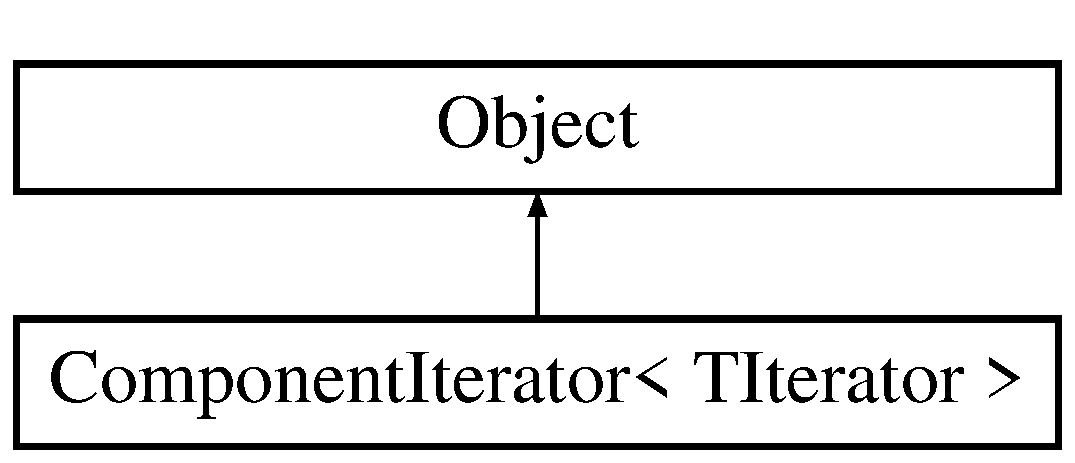
\includegraphics[height=2.000000cm]{structComponentIterator}
\end{center}
\end{figure}
\subsection*{Public Types}
\begin{DoxyCompactItemize}
\item 
\hypertarget{structComponentIterator_af45edea89e80969d8103d6ce3656cefa}{}\label{structComponentIterator_af45edea89e80969d8103d6ce3656cefa} 
using {\bfseries T} = decltype(($\ast$std\+::declval$<$ T\+Iterator $>$())\mbox{[}std\+::declval$<$ int $>$()\mbox{]})
\item 
\hypertarget{structComponentIterator_a87167d7c082b33956a1d8b27065ba5c9}{}\label{structComponentIterator_a87167d7c082b33956a1d8b27065ba5c9} 
using {\bfseries RawT} = std\+::decay\+\_\+t$<$ T $>$
\item 
\hypertarget{structComponentIterator_aad22d6594ae852e94079ffa2a5cae6de}{}\label{structComponentIterator_aad22d6594ae852e94079ffa2a5cae6de} 
using {\bfseries iterator\+\_\+category} = std\+::random\+\_\+access\+\_\+iterator\+\_\+tag
\item 
\hypertarget{structComponentIterator_a73e3b2634cef93a06ee942b0dbad9856}{}\label{structComponentIterator_a73e3b2634cef93a06ee942b0dbad9856} 
using {\bfseries value\+\_\+type} = RawT
\item 
\hypertarget{structComponentIterator_acc09c8bda29d100a3836e807287fc794}{}\label{structComponentIterator_acc09c8bda29d100a3836e807287fc794} 
using {\bfseries difference\+\_\+type} = size\+\_\+t
\item 
\hypertarget{structComponentIterator_aed6e70eb573fbe42ead1ca6b8e218592}{}\label{structComponentIterator_aed6e70eb573fbe42ead1ca6b8e218592} 
using {\bfseries pointer} = RawT $\ast$
\item 
\hypertarget{structComponentIterator_a7b37e257cad37ea01f8d1515909a71ec}{}\label{structComponentIterator_a7b37e257cad37ea01f8d1515909a71ec} 
using {\bfseries reference} = RawT \&
\end{DoxyCompactItemize}
\subsection*{Public Member Functions}
\begin{DoxyCompactItemize}
\item 
\hypertarget{structComponentIterator_a2e1cc666a2eaec6287ec612145491982}{}\label{structComponentIterator_a2e1cc666a2eaec6287ec612145491982} 
{\bfseries Component\+Iterator} (const T\+Iterator \&iterator, const int component)
\item 
\hypertarget{structComponentIterator_aa11f240d815ddceb4a3fb3a7a1b3ce36}{}\label{structComponentIterator_aa11f240d815ddceb4a3fb3a7a1b3ce36} 
const RawT \& {\bfseries operator$\ast$} () const
\item 
\hypertarget{structComponentIterator_a962ddbc9f6f44f82d366257ed574bf8f}{}\label{structComponentIterator_a962ddbc9f6f44f82d366257ed574bf8f} 
RawT \& {\bfseries operator$\ast$} ()
\item 
\hypertarget{structComponentIterator_a668af983401a19b0993e6f1335f6f789}{}\label{structComponentIterator_a668af983401a19b0993e6f1335f6f789} 
\hyperlink{structComponentIterator}{Component\+Iterator} \& {\bfseries operator++} ()
\item 
\hypertarget{structComponentIterator_a4877f1587d6526925355955bc7be882b}{}\label{structComponentIterator_a4877f1587d6526925355955bc7be882b} 
\hyperlink{structComponentIterator}{Component\+Iterator} {\bfseries operator++} (int)
\item 
\hypertarget{structComponentIterator_ab8ecc1d0d6f5c8e4ce22549939daec5d}{}\label{structComponentIterator_ab8ecc1d0d6f5c8e4ce22549939daec5d} 
\hyperlink{structComponentIterator}{Component\+Iterator} \& {\bfseries operator-\/-\/} ()
\item 
\hypertarget{structComponentIterator_a30169a624479f81ff980916bb77d5515}{}\label{structComponentIterator_a30169a624479f81ff980916bb77d5515} 
\hyperlink{structComponentIterator}{Component\+Iterator} {\bfseries operator-\/-\/} (int)
\item 
\hypertarget{structComponentIterator_a63ee4d99b185e9c17b216399b09f81f4}{}\label{structComponentIterator_a63ee4d99b185e9c17b216399b09f81f4} 
\hyperlink{structComponentIterator}{Component\+Iterator} {\bfseries operator+} (const int n) const
\item 
\hypertarget{structComponentIterator_af7113fe1670b698375ae29c6307368cb}{}\label{structComponentIterator_af7113fe1670b698375ae29c6307368cb} 
\hyperlink{structComponentIterator}{Component\+Iterator} {\bfseries operator-\/} (const int n) const
\item 
\hypertarget{structComponentIterator_aa31e6996dd188992bf3ead9c6e8de31b}{}\label{structComponentIterator_aa31e6996dd188992bf3ead9c6e8de31b} 
void {\bfseries operator+=} (const int n)
\item 
\hypertarget{structComponentIterator_a626ddae3b36436c8be60f08a485ca3e2}{}\label{structComponentIterator_a626ddae3b36436c8be60f08a485ca3e2} 
void {\bfseries operator-\/=} (const int n)
\item 
\hypertarget{structComponentIterator_a0ace5af59b7a28691e2c47aecd663925}{}\label{structComponentIterator_a0ace5af59b7a28691e2c47aecd663925} 
size\+\_\+t {\bfseries operator-\/} (const \hyperlink{structComponentIterator}{Component\+Iterator} \&other) const
\item 
\hypertarget{structComponentIterator_a7902a36a55188e90ec6dd2e29150d180}{}\label{structComponentIterator_a7902a36a55188e90ec6dd2e29150d180} 
bool {\bfseries operator$<$} (const \hyperlink{structComponentIterator}{Component\+Iterator} \&other) const
\item 
\hypertarget{structComponentIterator_a44d0db9c4573423b896f00bfebb42a45}{}\label{structComponentIterator_a44d0db9c4573423b896f00bfebb42a45} 
bool {\bfseries operator$>$} (const \hyperlink{structComponentIterator}{Component\+Iterator} \&other) const
\item 
\hypertarget{structComponentIterator_a52edd362550b70dc96a1f91251602645}{}\label{structComponentIterator_a52edd362550b70dc96a1f91251602645} 
bool {\bfseries operator$<$=} (const \hyperlink{structComponentIterator}{Component\+Iterator} \&other) const
\item 
\hypertarget{structComponentIterator_a9ad2cf77ccf9b33b59ae3e299e8d78e6}{}\label{structComponentIterator_a9ad2cf77ccf9b33b59ae3e299e8d78e6} 
bool {\bfseries operator$>$=} (const \hyperlink{structComponentIterator}{Component\+Iterator} \&other) const
\item 
\hypertarget{structComponentIterator_ac6ba955d23b2902d9b7a82582319b86b}{}\label{structComponentIterator_ac6ba955d23b2902d9b7a82582319b86b} 
bool {\bfseries operator==} (const \hyperlink{structComponentIterator}{Component\+Iterator} \&other)
\item 
\hypertarget{structComponentIterator_a512b0556981741aa1e3a8ec8c2aafd2b}{}\label{structComponentIterator_a512b0556981741aa1e3a8ec8c2aafd2b} 
bool {\bfseries operator!=} (const \hyperlink{structComponentIterator}{Component\+Iterator} \&other)
\end{DoxyCompactItemize}
\subsection*{Public Attributes}
\begin{DoxyCompactItemize}
\item 
\hypertarget{structComponentIterator_a9848900414c31afb41fd3426097cf24e}{}\label{structComponentIterator_a9848900414c31afb41fd3426097cf24e} 
T\+Iterator {\bfseries iterator}
\item 
\hypertarget{structComponentIterator_a7e530e5fea4c2dbd14287ee5efb78197}{}\label{structComponentIterator_a7e530e5fea4c2dbd14287ee5efb78197} 
int {\bfseries component}
\end{DoxyCompactItemize}


\subsection{Detailed Description}
\subsubsection*{template$<$typename T\+Iterator$>$\newline
struct Component\+Iterator$<$ T\+Iterator $>$}

\hyperlink{classIterator}{Iterator} adapters Pavel Sevecek 2016 sevecek at sirrah.\+troja.\+mff.\+cuni.\+cz 

The documentation for this struct was generated from the following file\+:\begin{DoxyCompactItemize}
\item 
/home/pavel/projects/astro/sph2/src/utils/iterators.\+h\end{DoxyCompactItemize}

\hypertarget{classConfigBlock}{}\section{Config\+Block Class Reference}
\label{classConfigBlock}\index{Config\+Block@{Config\+Block}}
Inheritance diagram for Config\+Block\+:\begin{figure}[H]
\begin{center}
\leavevmode
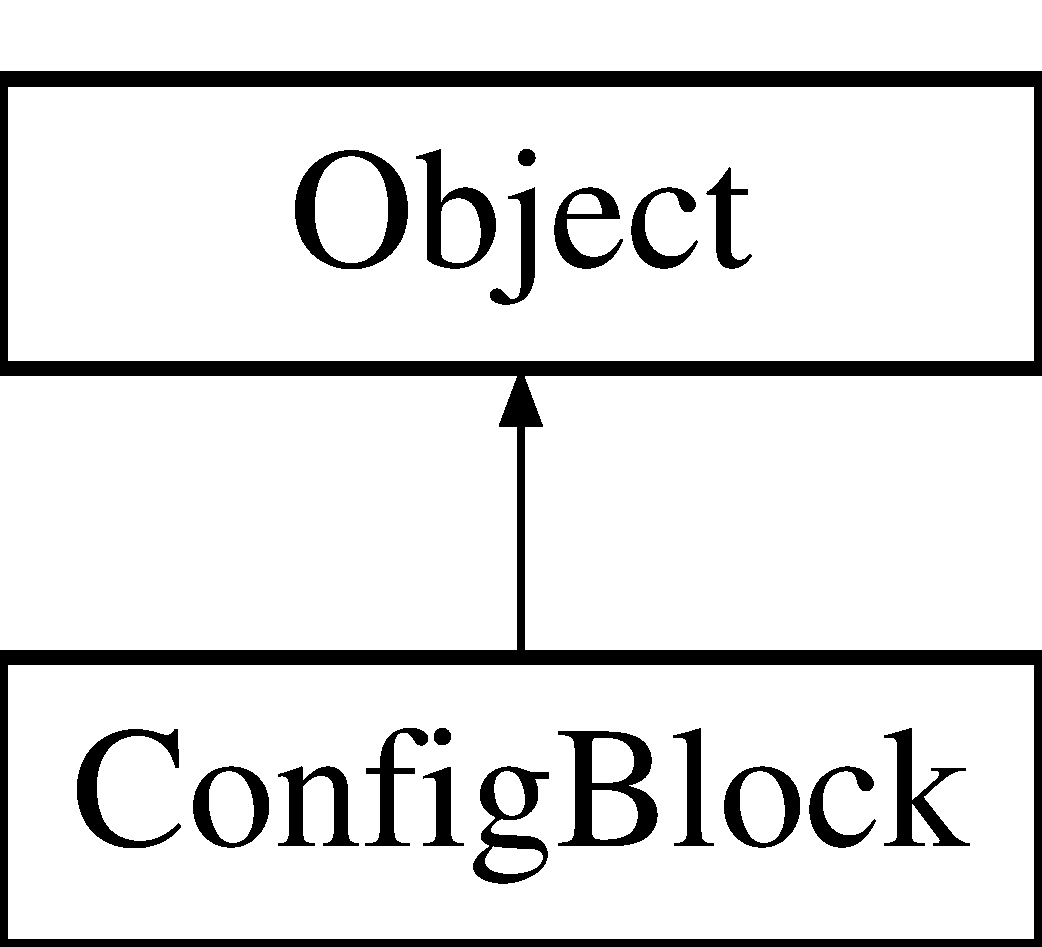
\includegraphics[height=2.000000cm]{classConfigBlock}
\end{center}
\end{figure}
\subsection*{Public Member Functions}
\begin{DoxyCompactItemize}
\item 
\hypertarget{classConfigBlock_a0acf7d5147a4a7ae965aca6da6c351ee}{}\label{classConfigBlock_a0acf7d5147a4a7ae965aca6da6c351ee} 
{\footnotesize template$<$typename T $>$ }\\void {\bfseries add} (const std\+::string \&name, T \&\&value)
\item 
\hypertarget{classConfigBlock_a3b26fa398f831adee695d71f8095ed26}{}\label{classConfigBlock_a3b26fa398f831adee695d71f8095ed26} 
bool {\bfseries write} (const std\+::string \&path)
\end{DoxyCompactItemize}
\subsection*{Friends}
\begin{DoxyCompactItemize}
\item 
\hypertarget{classConfigBlock_a4d53249f3dd66a65e783fc86bcebdfd3}{}\label{classConfigBlock_a4d53249f3dd66a65e783fc86bcebdfd3} 
class {\bfseries Config\+Visitor}
\end{DoxyCompactItemize}


The documentation for this class was generated from the following file\+:\begin{DoxyCompactItemize}
\item 
/home/pavel/projects/astro/sph2/src/parser/parse.\+h\end{DoxyCompactItemize}

\hypertarget{classConfigValue}{}\section{Config\+Value Class Reference}
\label{classConfigValue}\index{Config\+Value@{Config\+Value}}
Inheritance diagram for Config\+Value\+:\begin{figure}[H]
\begin{center}
\leavevmode
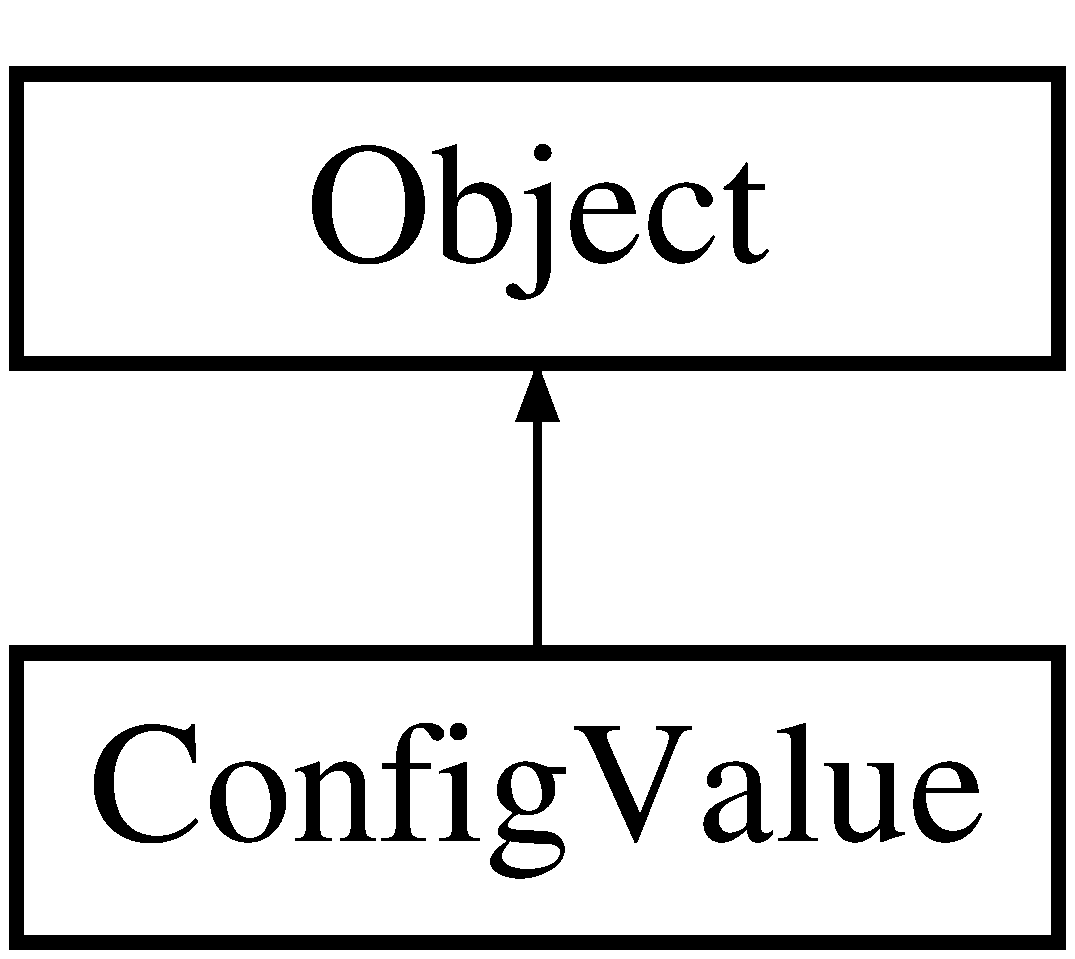
\includegraphics[height=2.000000cm]{classConfigValue}
\end{center}
\end{figure}
\subsection*{Public Member Functions}
\begin{DoxyCompactItemize}
\item 
\hypertarget{classConfigValue_a609063f010e809bbfe0ba17169e73d0a}{}\label{classConfigValue_a609063f010e809bbfe0ba17169e73d0a} 
\hyperlink{classConfigValue_a609063f010e809bbfe0ba17169e73d0a}{Config\+Value} (const std\+::string \&line)
\begin{DoxyCompactList}\small\item\em Constructs the value from a line of config file. \end{DoxyCompactList}\end{DoxyCompactItemize}


The documentation for this class was generated from the following file\+:\begin{DoxyCompactItemize}
\item 
/home/pavel/projects/astro/sph2/src/parser/parse.\+h\end{DoxyCompactItemize}

\hypertarget{structConfigVisitor}{}\section{Config\+Visitor Struct Reference}
\label{structConfigVisitor}\index{Config\+Visitor@{Config\+Visitor}}
\subsection*{Public Member Functions}
\begin{DoxyCompactItemize}
\item 
\hypertarget{structConfigVisitor_a83ebb8de13b12b6c7455975c60c0a50c}{}\label{structConfigVisitor_a83ebb8de13b12b6c7455975c60c0a50c} 
{\footnotesize template$<$typename T $>$ }\\void {\bfseries operator()} (T \&\&value)
\item 
\hypertarget{structConfigVisitor_a976934913e7993d15131c503d753a30b}{}\label{structConfigVisitor_a976934913e7993d15131c503d753a30b} 
void {\bfseries operator()} (std\+::shared\+\_\+ptr$<$ \hyperlink{classConfigBlock}{Config\+Block} $>$ \&sub\+Block)
\item 
\hypertarget{structConfigVisitor_a43ea135adb36aeccf57e12b7ef18bcc3}{}\label{structConfigVisitor_a43ea135adb36aeccf57e12b7ef18bcc3} 
{\bfseries Config\+Visitor} (std\+::ofstream \&ofs, \hyperlink{classConfigBlock}{Config\+Block} $\ast$parent, int depth)
\end{DoxyCompactItemize}
\subsection*{Public Attributes}
\begin{DoxyCompactItemize}
\item 
\hypertarget{structConfigVisitor_a641d48a6c2b982acec6c09156605e1ee}{}\label{structConfigVisitor_a641d48a6c2b982acec6c09156605e1ee} 
std\+::ofstream \& {\bfseries ofs}
\item 
\hypertarget{structConfigVisitor_a058be8370eed8587f90cbe6c5fc64549}{}\label{structConfigVisitor_a058be8370eed8587f90cbe6c5fc64549} 
\hyperlink{classConfigBlock}{Config\+Block} $\ast$ {\bfseries parent}
\item 
\hypertarget{structConfigVisitor_aa45d134c8e26ad6b011d46751d90e1bf}{}\label{structConfigVisitor_aa45d134c8e26ad6b011d46751d90e1bf} 
int {\bfseries depth}
\end{DoxyCompactItemize}


The documentation for this struct was generated from the following file\+:\begin{DoxyCompactItemize}
\item 
/home/pavel/projects/astro/sph2/src/parser/parse.\+h\end{DoxyCompactItemize}

\hypertarget{structConstructType}{}\section{Construct\+Type$<$ n, T0, T\+Args $>$ Struct Template Reference}
\label{structConstructType}\index{Construct\+Type$<$ n, T0, T\+Args $>$@{Construct\+Type$<$ n, T0, T\+Args $>$}}


Constucts type given by runtime index.  




{\ttfamily \#include $<$variant.\+old.\+h$>$}

\subsection*{Static Public Member Functions}
\begin{DoxyCompactItemize}
\item 
\hypertarget{structConstructType_acdc048e3ce2a7411b7b16d2fb5d3139e}{}\label{structConstructType_acdc048e3ce2a7411b7b16d2fb5d3139e} 
{\footnotesize template$<$typename T $>$ }\\static void {\bfseries action} (const int idx, char $\ast$data, T \&\&value)
\end{DoxyCompactItemize}


\subsection{Detailed Description}
\subsubsection*{template$<$int n, typename T0, typename... T\+Args$>$\newline
struct Construct\+Type$<$ n, T0, T\+Args $>$}

Constucts type given by runtime index. 

The documentation for this struct was generated from the following file\+:\begin{DoxyCompactItemize}
\item 
/home/pavel/projects/astro/sph2/src/structs/variant.\+old.\+h\end{DoxyCompactItemize}

\hypertarget{structConstructType_3_01n_00_01T0_01_4}{}\section{Construct\+Type$<$ n, T0 $>$ Struct Template Reference}
\label{structConstructType_3_01n_00_01T0_01_4}\index{Construct\+Type$<$ n, T0 $>$@{Construct\+Type$<$ n, T0 $>$}}
\subsection*{Static Public Member Functions}
\begin{DoxyCompactItemize}
\item 
\hypertarget{structConstructType_3_01n_00_01T0_01_4_a7c2521d2c0fec2b8d35fe075e0fce526}{}\label{structConstructType_3_01n_00_01T0_01_4_a7c2521d2c0fec2b8d35fe075e0fce526} 
{\footnotesize template$<$typename T $>$ }\\static void {\bfseries action} (const int idx, char $\ast$data, T \&\&value)
\end{DoxyCompactItemize}


The documentation for this struct was generated from the following file\+:\begin{DoxyCompactItemize}
\item 
/home/pavel/projects/astro/sph2/src/structs/variant.\+old.\+h\end{DoxyCompactItemize}

\hypertarget{classCubicPacking}{}\section{Cubic\+Packing Class Reference}
\label{classCubicPacking}\index{Cubic\+Packing@{Cubic\+Packing}}


Cubic close packing.  




{\ttfamily \#include $<$initconds.\+h$>$}

Inheritance diagram for Cubic\+Packing\+:\begin{figure}[H]
\begin{center}
\leavevmode
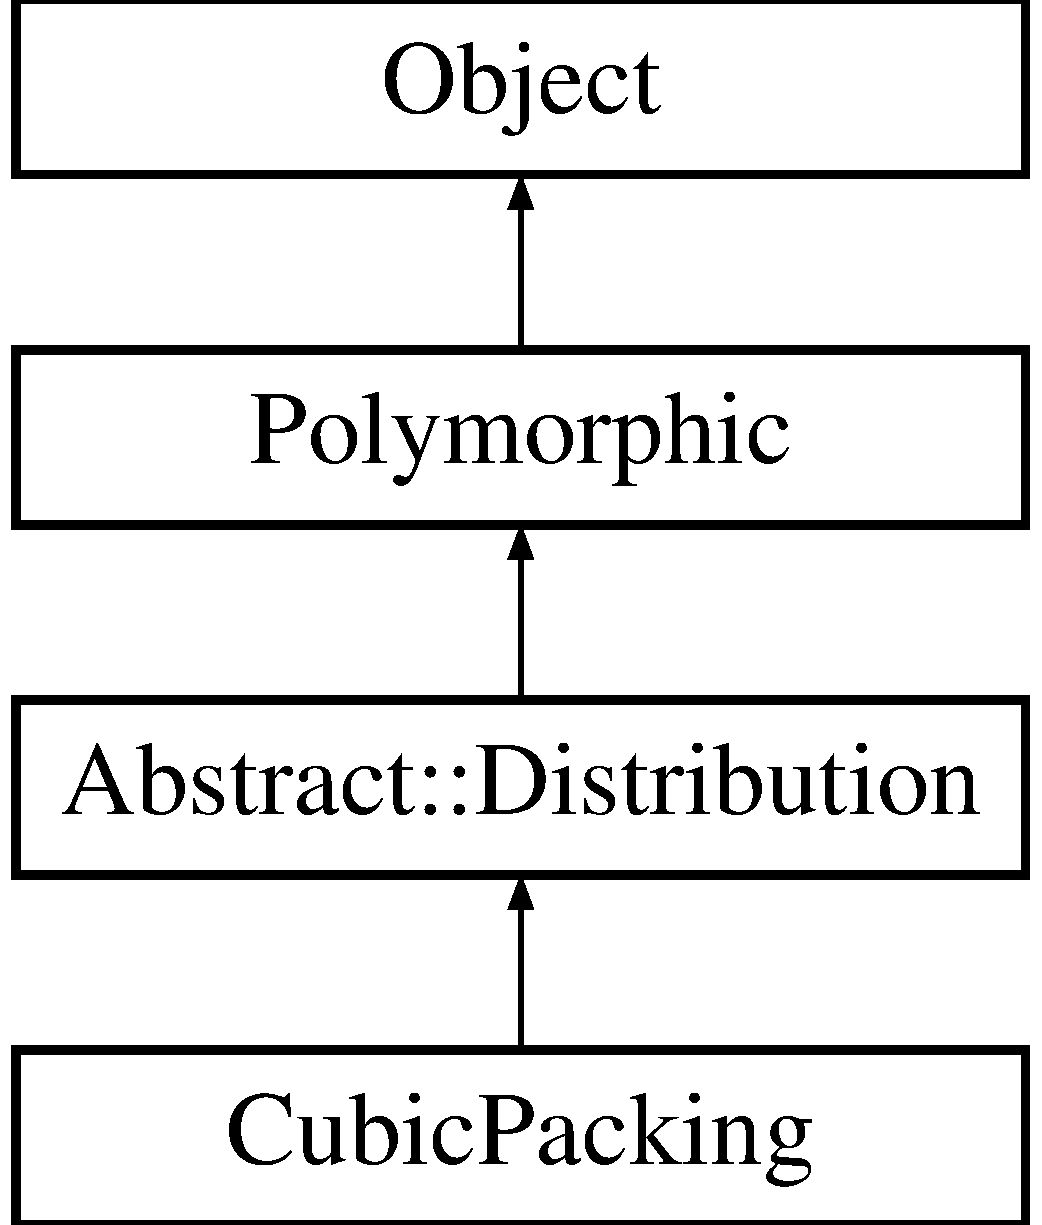
\includegraphics[height=4.000000cm]{classCubicPacking}
\end{center}
\end{figure}
\subsection*{Public Member Functions}
\begin{DoxyCompactItemize}
\item 
virtual \hyperlink{classArray}{Array}$<$ \hyperlink{classBasicVector}{Vector} $>$ \hyperlink{classCubicPacking_aa3c9a226ffa03b38a7b5fedad1414a01}{generate} (const int n, const \hyperlink{classAbstract_1_1Domain}{Abstract\+::\+Domain} $\ast$domain) const override
\end{DoxyCompactItemize}


\subsection{Detailed Description}
Cubic close packing. 

\subsection{Member Function Documentation}
\hypertarget{classCubicPacking_aa3c9a226ffa03b38a7b5fedad1414a01}{}\label{classCubicPacking_aa3c9a226ffa03b38a7b5fedad1414a01} 
\index{Cubic\+Packing@{Cubic\+Packing}!generate@{generate}}
\index{generate@{generate}!Cubic\+Packing@{Cubic\+Packing}}
\subsubsection{\texorpdfstring{generate()}{generate()}}
{\footnotesize\ttfamily virtual \hyperlink{classArray}{Array}$<$\hyperlink{classBasicVector}{Vector}$>$ Cubic\+Packing\+::generate (\begin{DoxyParamCaption}\item[{const int}]{n,  }\item[{const \hyperlink{classAbstract_1_1Domain}{Abstract\+::\+Domain} $\ast$}]{domain }\end{DoxyParamCaption}) const\hspace{0.3cm}{\ttfamily [inline]}, {\ttfamily [override]}, {\ttfamily [virtual]}}

Base class for generating vertices with specific distribution. Also generates corresponding smoothing lengths and save them as fourth component of the vector. 
\begin{DoxyParams}{Parameters}
{\em n} & Expected number of generated vertices. \\
\hline
{\em domain} & Computational domain where the vertices are distributed \\
\hline
\end{DoxyParams}
\begin{DoxyReturn}{Returns}
Output array of vertices. The total number of vertices can slightly differ from n. 
\end{DoxyReturn}
\begin{DoxyNote}{Note}
This method is expected to be called once at the beginning of the run, so we can return allocated array without worrying about performance costs here. 
\end{DoxyNote}
\begin{DoxyRefDesc}{Todo}
\item[\hyperlink{todo__todo000013}{Todo}]better estimate of how many we need to allocate, or reallocation like std\+::vector \end{DoxyRefDesc}


Implements \hyperlink{classAbstract_1_1Distribution_aefb835b4c4d2d0a5f864bc2cee0492b2}{Abstract\+::\+Distribution}.



The documentation for this class was generated from the following file\+:\begin{DoxyCompactItemize}
\item 
/home/pavel/projects/astro/sph2/src/initconds/initconds.\+h\end{DoxyCompactItemize}

\hypertarget{classCubicSpline}{}\section{Cubic\+Spline Class Reference}
\label{classCubicSpline}\index{Cubic\+Spline@{Cubic\+Spline}}


A cubic spline (M4) kernel.  




{\ttfamily \#include $<$kernel.\+h$>$}

Inheritance diagram for Cubic\+Spline\+:\begin{figure}[H]
\begin{center}
\leavevmode
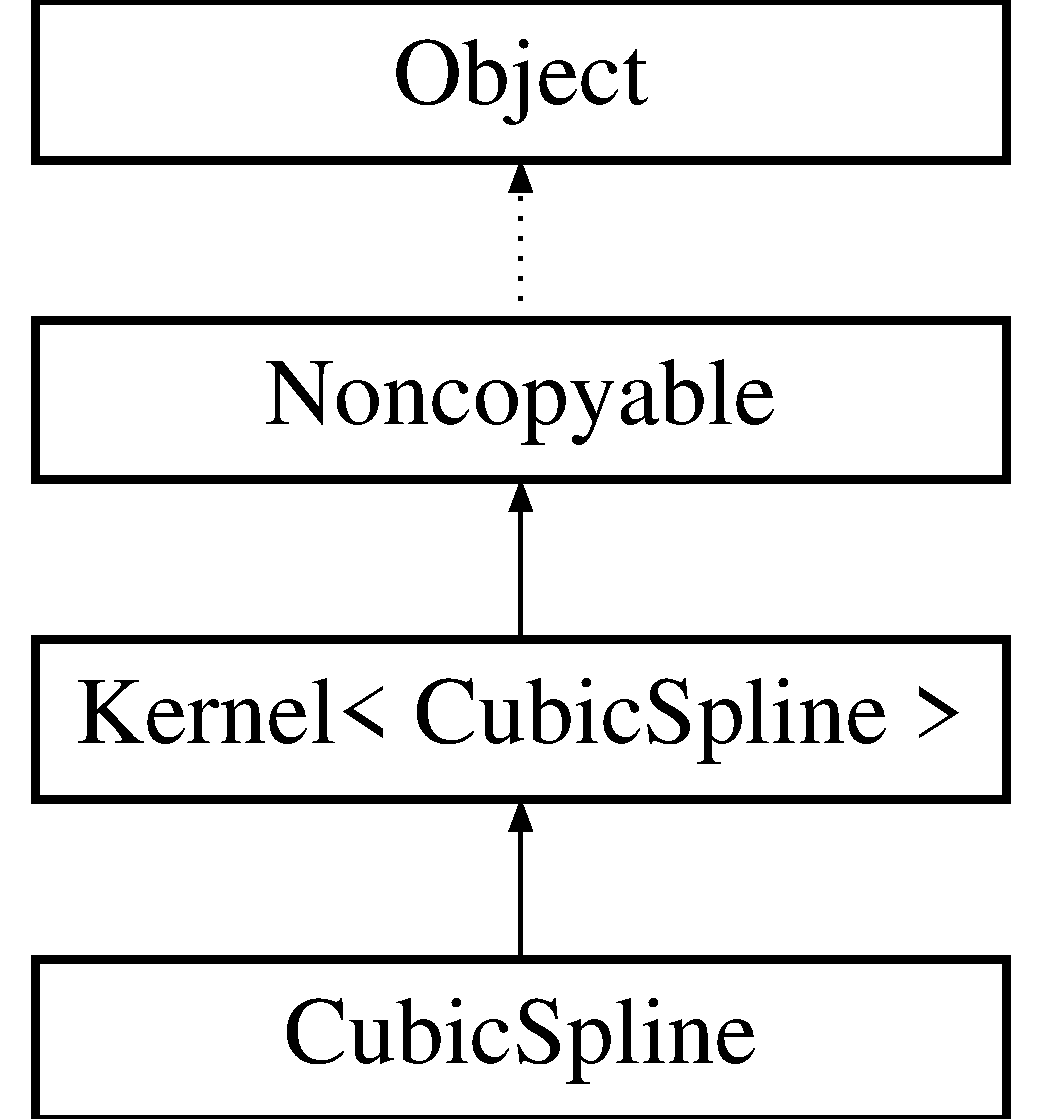
\includegraphics[height=4.000000cm]{classCubicSpline}
\end{center}
\end{figure}
\subsection*{Public Member Functions}
\begin{DoxyCompactItemize}
\item 
\hypertarget{classCubicSpline_abb48f59e3708ac00f1dbb10b5a34307d}{}\label{classCubicSpline_abb48f59e3708ac00f1dbb10b5a34307d} 
I\+N\+L\+I\+NE Float {\bfseries radius} () const
\item 
\hypertarget{classCubicSpline_ad3704f560df9a5dda63d249e38413f74}{}\label{classCubicSpline_ad3704f560df9a5dda63d249e38413f74} 
I\+N\+L\+I\+NE Float {\bfseries value\+Impl} (const Float \&q\+Sqr) const
\item 
\hypertarget{classCubicSpline_ab88666d41a68234882a028cba969551a}{}\label{classCubicSpline_ab88666d41a68234882a028cba969551a} 
I\+N\+L\+I\+NE Float {\bfseries grad\+Impl} (const Float \&q\+Sqr) const
\end{DoxyCompactItemize}


\subsection{Detailed Description}
A cubic spline (M4) kernel. 

The documentation for this class was generated from the following file\+:\begin{DoxyCompactItemize}
\item 
/home/pavel/projects/astro/sph2/src/kernel/kernel.\+h\end{DoxyCompactItemize}

\hypertarget{classDataFile}{}\section{Data\+File$<$ T\+Args $>$ Class Template Reference}
\label{classDataFile}\index{Data\+File$<$ T\+Args $>$@{Data\+File$<$ T\+Args $>$}}


{\ttfamily \#include $<$parse.\+h$>$}

Inheritance diagram for Data\+File$<$ T\+Args $>$\+:\begin{figure}[H]
\begin{center}
\leavevmode
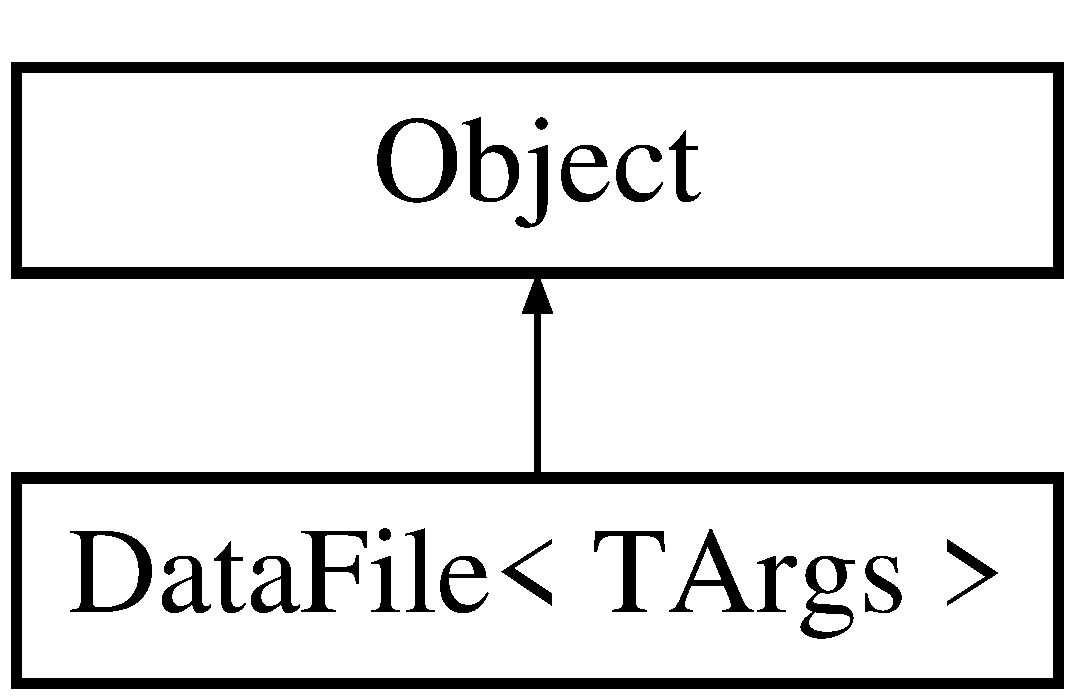
\includegraphics[height=2.000000cm]{classDataFile}
\end{center}
\end{figure}
\subsection*{Public Member Functions}
\begin{DoxyCompactItemize}
\item 
\hypertarget{classDataFile_a39baec6df72d09c9fc17ce1448e434ed}{}\label{classDataFile_a39baec6df72d09c9fc17ce1448e434ed} 
\hyperlink{classArray}{Array}$<$ \hyperlink{classTuple}{Tuple}$<$ T\+Args... $>$ $>$ {\bfseries load} (const std\+::string \&path)
\item 
\hypertarget{classDataFile_ae4cfc73ee9970372638ccb9fe8a2ce25}{}\label{classDataFile_ae4cfc73ee9970372638ccb9fe8a2ce25} 
void \hyperlink{classDataFile_ae4cfc73ee9970372638ccb9fe8a2ce25}{save} (const \hyperlink{classArray}{Array}$<$ \hyperlink{classTuple}{Tuple}$<$ T\+Args... $>$$>$ \&array, const std\+::string \&path)
\begin{DoxyCompactList}\small\item\em Save array of tuples with the same arguments as the file. \end{DoxyCompactList}\item 
{\footnotesize template$<$typename T $>$ }\\void \hyperlink{classDataFile_a2ed8b7e88e74a459050959b782008821}{save} (const \hyperlink{classArray}{Array}$<$ T $>$ \&array, const std\+::string \&path, Saving\+Options options=Saving\+Options\+::\+N\+O\+\_\+\+U\+N\+I\+TS)
\item 
\hypertarget{classDataFile_a05882080cb1a937a64d6777600e8bc50}{}\label{classDataFile_a05882080cb1a937a64d6777600e8bc50} 
void \hyperlink{classDataFile_a05882080cb1a937a64d6777600e8bc50}{save} (const std\+::string \&path, const \hyperlink{classArray}{Array}$<$ T\+Args $>$ \&... arrays)
\begin{DoxyCompactList}\small\item\em \hyperlink{classTuple}{Tuple} of arrays. \end{DoxyCompactList}\end{DoxyCompactItemize}


\subsection{Detailed Description}
\subsubsection*{template$<$typename... T\+Args$>$\newline
class Data\+File$<$ T\+Args $>$}

Loading/saving array of generic data from/into textfiles. A column of file are determined by template parameters of the class. Can save/load any kind of data as long as operators $>$$>$ and $<$$<$ exist. T\+O\+DO\+: ignore \textquotesingle{}\#\textquotesingle{} lines when loading 

\subsection{Member Function Documentation}
\hypertarget{classDataFile_a2ed8b7e88e74a459050959b782008821}{}\label{classDataFile_a2ed8b7e88e74a459050959b782008821} 
\index{Data\+File@{Data\+File}!save@{save}}
\index{save@{save}!Data\+File@{Data\+File}}
\subsubsection{\texorpdfstring{save()}{save()}}
{\footnotesize\ttfamily template$<$typename... T\+Args$>$ \\
template$<$typename T $>$ \\
void \hyperlink{classDataFile}{Data\+File}$<$ T\+Args $>$\+::save (\begin{DoxyParamCaption}\item[{const \hyperlink{classArray}{Array}$<$ T $>$ \&}]{array,  }\item[{const std\+::string \&}]{path,  }\item[{Saving\+Options}]{options = {\ttfamily SavingOptions\+:\+:NO\+\_\+UNITS} }\end{DoxyParamCaption})\hspace{0.3cm}{\ttfamily [inline]}}

Save an array of any type T that has \mbox{[}\mbox{]} operator and static constexpr int \textquotesingle{}dimensions\textquotesingle{}. Taylored for easily saving array of vectors. 

The documentation for this class was generated from the following file\+:\begin{DoxyCompactItemize}
\item 
/home/pavel/projects/astro/sph2/src/parser/parse.\+h\end{DoxyCompactItemize}

\hypertarget{classDateFormat}{}\section{Date\+Format Class Reference}
\label{classDateFormat}\index{Date\+Format@{Date\+Format}}
Inheritance diagram for Date\+Format\+:\begin{figure}[H]
\begin{center}
\leavevmode
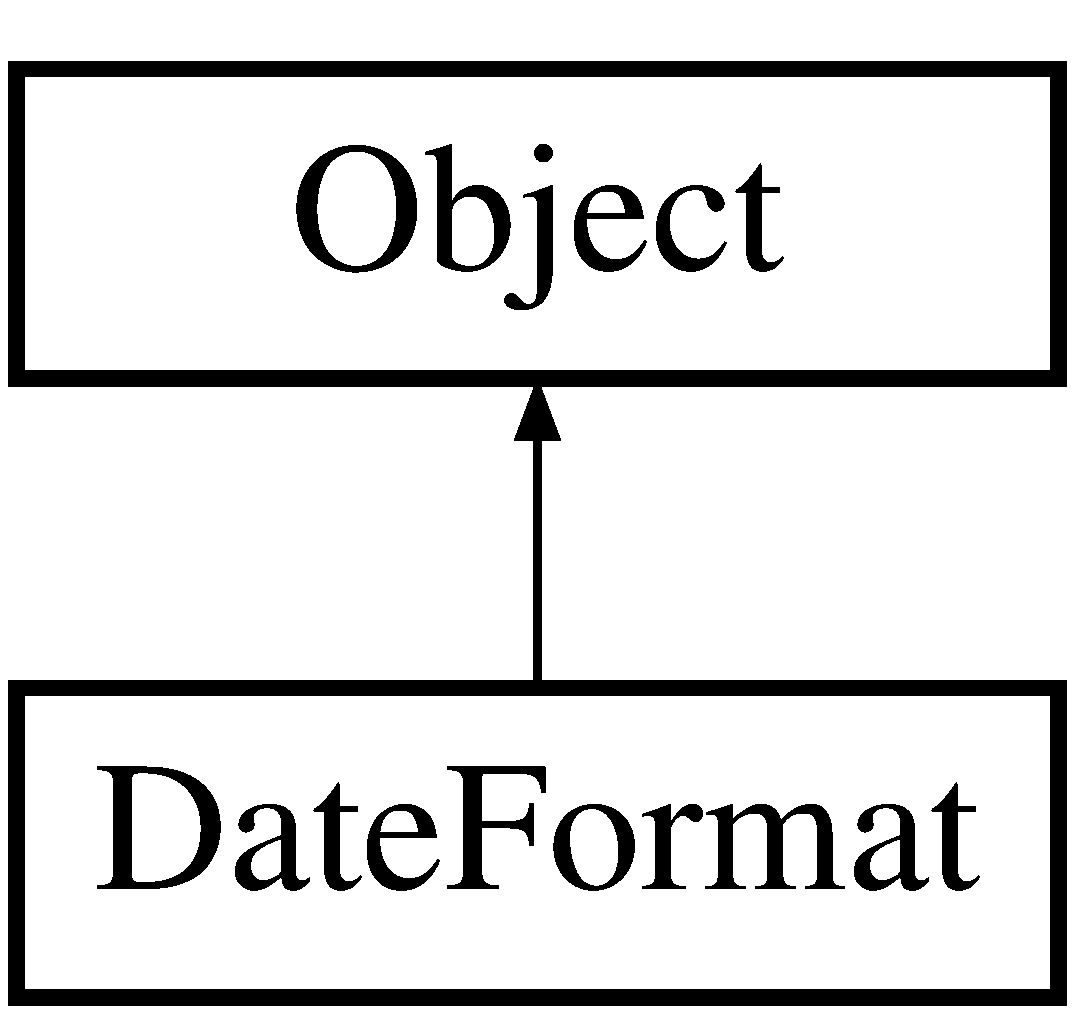
\includegraphics[height=2.000000cm]{classDateFormat}
\end{center}
\end{figure}
\subsection*{Public Member Functions}
\begin{DoxyCompactItemize}
\item 
\hypertarget{classDateFormat_a4a44523d5371920bbb4967fce29a9544}{}\label{classDateFormat_a4a44523d5371920bbb4967fce29a9544} 
{\bfseries Date\+Format} (const Float value, const Julian\+Date\+Format input\+Format, const std\+::string \&output\+Format)
\item 
\hypertarget{classDateFormat_ab391ba82767ede94c6951e1ba61afcef}{}\label{classDateFormat_ab391ba82767ede94c6951e1ba61afcef} 
std\+::string {\bfseries get} () const
\end{DoxyCompactItemize}


The documentation for this class was generated from the following file\+:\begin{DoxyCompactItemize}
\item 
/home/pavel/projects/astro/sph2/src/physics/timeformat.\+h\end{DoxyCompactItemize}

\hypertarget{classAbstract_1_1Distribution}{}\section{Abstract\+:\+:Distribution Class Reference}
\label{classAbstract_1_1Distribution}\index{Abstract\+::\+Distribution@{Abstract\+::\+Distribution}}
Inheritance diagram for Abstract\+:\+:Distribution\+:\begin{figure}[H]
\begin{center}
\leavevmode
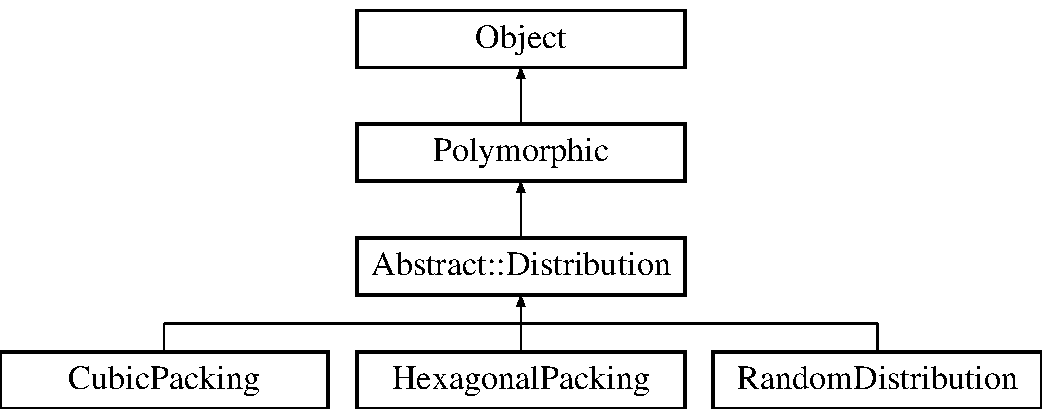
\includegraphics[height=4.000000cm]{classAbstract_1_1Distribution}
\end{center}
\end{figure}
\subsection*{Public Member Functions}
\begin{DoxyCompactItemize}
\item 
virtual \hyperlink{classArray}{Array}$<$ \hyperlink{classBasicVector}{Vector} $>$ \hyperlink{classAbstract_1_1Distribution_aefb835b4c4d2d0a5f864bc2cee0492b2}{generate} (const int n, const \hyperlink{classAbstract_1_1Domain}{Domain} $\ast$domain) const =0
\end{DoxyCompactItemize}


\subsection{Member Function Documentation}
\hypertarget{classAbstract_1_1Distribution_aefb835b4c4d2d0a5f864bc2cee0492b2}{}\label{classAbstract_1_1Distribution_aefb835b4c4d2d0a5f864bc2cee0492b2} 
\index{Abstract\+::\+Distribution@{Abstract\+::\+Distribution}!generate@{generate}}
\index{generate@{generate}!Abstract\+::\+Distribution@{Abstract\+::\+Distribution}}
\subsubsection{\texorpdfstring{generate()}{generate()}}
{\footnotesize\ttfamily virtual \hyperlink{classArray}{Array}$<$\hyperlink{classBasicVector}{Vector}$>$ Abstract\+::\+Distribution\+::generate (\begin{DoxyParamCaption}\item[{const int}]{n,  }\item[{const \hyperlink{classAbstract_1_1Domain}{Domain} $\ast$}]{domain }\end{DoxyParamCaption}) const\hspace{0.3cm}{\ttfamily [pure virtual]}}

Base class for generating vertices with specific distribution. Also generates corresponding smoothing lengths and save them as fourth component of the vector. 
\begin{DoxyParams}{Parameters}
{\em n} & Expected number of generated vertices. \\
\hline
{\em domain} & Computational domain where the vertices are distributed \\
\hline
\end{DoxyParams}
\begin{DoxyReturn}{Returns}
Output array of vertices. The total number of vertices can slightly differ from n. 
\end{DoxyReturn}
\begin{DoxyNote}{Note}
This method is expected to be called once at the beginning of the run, so we can return allocated array without worrying about performance costs here. 
\end{DoxyNote}


Implemented in \hyperlink{classHexagonalPacking_a276079137928da5c94f8bb870b038c4a}{Hexagonal\+Packing}, \hyperlink{classCubicPacking_aa3c9a226ffa03b38a7b5fedad1414a01}{Cubic\+Packing}, and \hyperlink{classRandomDistribution_a3e1308d2bb28c5801e6e0537a8002597}{Random\+Distribution}.



The documentation for this class was generated from the following file\+:\begin{DoxyCompactItemize}
\item 
/home/pavel/projects/astro/sph2/src/initconds/initconds.\+h\end{DoxyCompactItemize}

\hypertarget{classAbstract_1_1Domain}{}\section{Abstract\+:\+:Domain Class Reference}
\label{classAbstract_1_1Domain}\index{Abstract\+::\+Domain@{Abstract\+::\+Domain}}


Class for defining computational domain.  




{\ttfamily \#include $<$domain.\+h$>$}

Inheritance diagram for Abstract\+:\+:Domain\+:\begin{figure}[H]
\begin{center}
\leavevmode
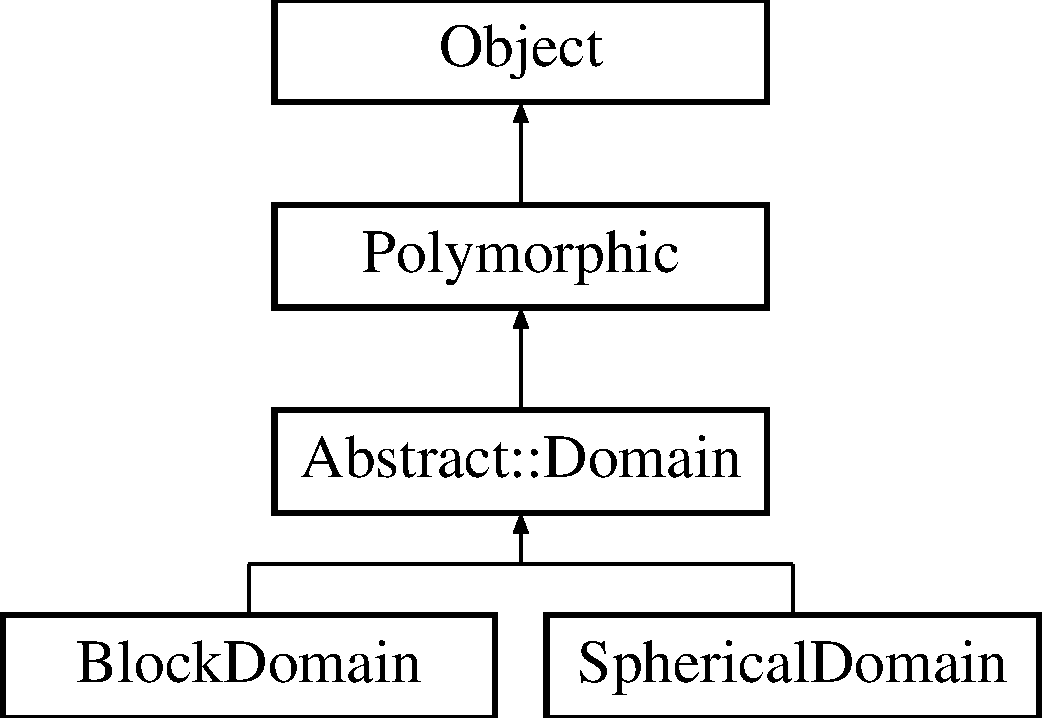
\includegraphics[height=4.000000cm]{classAbstract_1_1Domain}
\end{center}
\end{figure}
\subsection*{Public Member Functions}
\begin{DoxyCompactItemize}
\item 
\hypertarget{classAbstract_1_1Domain_a6c974123492230c334468091cefa66dd}{}\label{classAbstract_1_1Domain_a6c974123492230c334468091cefa66dd} 
\hyperlink{classAbstract_1_1Domain_a6c974123492230c334468091cefa66dd}{Domain} (const \hyperlink{classBasicVector}{Vector} \&center, const Float \&max\+Radius)
\begin{DoxyCompactList}\small\item\em Constructs the domain given its center point and a radius of a sphere containing the whole domain. \end{DoxyCompactList}\item 
\hypertarget{classAbstract_1_1Domain_a49180d7f20dc6eda9a7798a0052d4114}{}\label{classAbstract_1_1Domain_a49180d7f20dc6eda9a7798a0052d4114} 
virtual \hyperlink{classBasicVector}{Vector} \hyperlink{classAbstract_1_1Domain_a49180d7f20dc6eda9a7798a0052d4114}{get\+Center} () const
\begin{DoxyCompactList}\small\item\em Returns the center of the domain. \end{DoxyCompactList}\item 
\hypertarget{classAbstract_1_1Domain_afa2c3a29f56b31e35613b05078918f9f}{}\label{classAbstract_1_1Domain_afa2c3a29f56b31e35613b05078918f9f} 
virtual Float \hyperlink{classAbstract_1_1Domain_afa2c3a29f56b31e35613b05078918f9f}{get\+Bounding\+Radius} () const
\begin{DoxyCompactList}\small\item\em Returns the bounding radius of the domain. \end{DoxyCompactList}\item 
\hypertarget{classAbstract_1_1Domain_aa1e2803ef3f90984bdb82e46df32a082}{}\label{classAbstract_1_1Domain_aa1e2803ef3f90984bdb82e46df32a082} 
virtual Float \hyperlink{classAbstract_1_1Domain_aa1e2803ef3f90984bdb82e46df32a082}{get\+Volume} () const =0
\begin{DoxyCompactList}\small\item\em Returns the total d-\/dimensional volume of the domain. \end{DoxyCompactList}\item 
\hypertarget{classAbstract_1_1Domain_ac562e4b29568a1572b01853d5809e87f}{}\label{classAbstract_1_1Domain_ac562e4b29568a1572b01853d5809e87f} 
virtual bool \hyperlink{classAbstract_1_1Domain_ac562e4b29568a1572b01853d5809e87f}{is\+Inside} (const \hyperlink{classBasicVector}{Vector} \&v) const =0
\begin{DoxyCompactList}\small\item\em Checks if the vector lies inside the domain. \end{DoxyCompactList}\item 
virtual void \hyperlink{classAbstract_1_1Domain_a48ecb4ac3dab5f5a5e2de7b8e8218317}{are\+Inside} (const \hyperlink{classArrayView}{Array\+View}$<$ \hyperlink{classBasicVector}{Vector} $>$ vs, \hyperlink{classArrayView}{Array\+View}$<$ bool $>$ output) const =0
\item 
\hypertarget{classAbstract_1_1Domain_a25ad605750373faf0ade3d197187bc16}{}\label{classAbstract_1_1Domain_a25ad605750373faf0ade3d197187bc16} 
virtual void \hyperlink{classAbstract_1_1Domain_a25ad605750373faf0ade3d197187bc16}{project} (\hyperlink{classArrayView}{Array\+View}$<$ \hyperlink{classBasicVector}{Vector} $>$ vs) const =0
\begin{DoxyCompactList}\small\item\em Projects vectors outside of the domain onto its boundary. Vectors inside the domains are untouched. \end{DoxyCompactList}\end{DoxyCompactItemize}
\subsection*{Protected Attributes}
\begin{DoxyCompactItemize}
\item 
\hypertarget{classAbstract_1_1Domain_adc24a9392e0afc760beb51502baa9c0b}{}\label{classAbstract_1_1Domain_adc24a9392e0afc760beb51502baa9c0b} 
\hyperlink{classBasicVector}{Vector} {\bfseries center}
\item 
\hypertarget{classAbstract_1_1Domain_afe14973fe813d9c5ec25927faf1873f7}{}\label{classAbstract_1_1Domain_afe14973fe813d9c5ec25927faf1873f7} 
Float {\bfseries max\+Radius}
\end{DoxyCompactItemize}


\subsection{Detailed Description}
Class for defining computational domain. 

\subsection{Member Function Documentation}
\hypertarget{classAbstract_1_1Domain_a48ecb4ac3dab5f5a5e2de7b8e8218317}{}\label{classAbstract_1_1Domain_a48ecb4ac3dab5f5a5e2de7b8e8218317} 
\index{Abstract\+::\+Domain@{Abstract\+::\+Domain}!are\+Inside@{are\+Inside}}
\index{are\+Inside@{are\+Inside}!Abstract\+::\+Domain@{Abstract\+::\+Domain}}
\subsubsection{\texorpdfstring{are\+Inside()}{areInside()}}
{\footnotesize\ttfamily virtual void Abstract\+::\+Domain\+::are\+Inside (\begin{DoxyParamCaption}\item[{const \hyperlink{classArrayView}{Array\+View}$<$ \hyperlink{classBasicVector}{Vector} $>$}]{vs,  }\item[{\hyperlink{classArrayView}{Array\+View}$<$ bool $>$}]{output }\end{DoxyParamCaption}) const\hspace{0.3cm}{\ttfamily [pure virtual]}}

Checks if elements of an array are inside the domain. Returns the result as array of bools. \hyperlink{classArray}{Array} must be already allocated and its size must match array vs. 

Implemented in \hyperlink{classBlockDomain_a2dba56e9bbecdc5954147accfdcf331b}{Block\+Domain}, and \hyperlink{classSphericalDomain_aa5f4f17ecc1fa454da8b30e55bba98bf}{Spherical\+Domain}.



The documentation for this class was generated from the following file\+:\begin{DoxyCompactItemize}
\item 
/home/pavel/projects/astro/sph2/src/geometry/domain.\+h\end{DoxyCompactItemize}

\hypertarget{classDummyReferenceMaker}{}\section{Dummy\+Reference\+Maker$<$ T $>$ Class Template Reference}
\label{classDummyReferenceMaker}\index{Dummy\+Reference\+Maker$<$ T $>$@{Dummy\+Reference\+Maker$<$ T $>$}}
Inheritance diagram for Dummy\+Reference\+Maker$<$ T $>$\+:\begin{figure}[H]
\begin{center}
\leavevmode
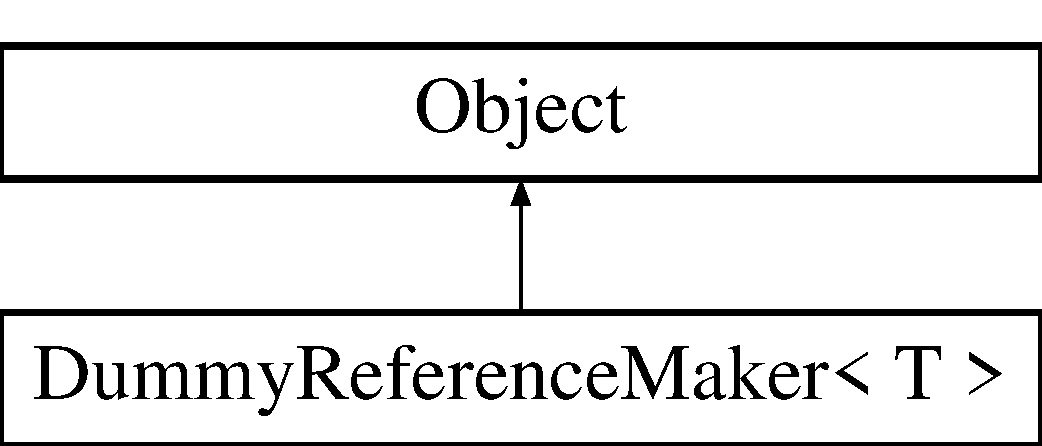
\includegraphics[height=2.000000cm]{classDummyReferenceMaker}
\end{center}
\end{figure}
\subsection*{Public Member Functions}
\begin{DoxyCompactItemize}
\item 
\hypertarget{classDummyReferenceMaker_a59727e1d1163a8b9ebb5656876a334c5}{}\label{classDummyReferenceMaker_a59727e1d1163a8b9ebb5656876a334c5} 
{\bfseries Dummy\+Reference\+Maker} (const T \&value)
\item 
\hypertarget{classDummyReferenceMaker_a918fa903ab4c1be5cf8195aa6d2ad7fc}{}\label{classDummyReferenceMaker_a918fa903ab4c1be5cf8195aa6d2ad7fc} 
{\bfseries operator T \&} ()
\item 
\hypertarget{classDummyReferenceMaker_a20e7ebcf7570c180e2d70fca01cc7392}{}\label{classDummyReferenceMaker_a20e7ebcf7570c180e2d70fca01cc7392} 
{\bfseries operator std\+::reference\+\_\+wrapper$<$ T $>$} ()
\end{DoxyCompactItemize}


The documentation for this class was generated from the following file\+:\begin{DoxyCompactItemize}
\item 
/home/pavel/projects/astro/sph2/src/geometry/indices.\+h\end{DoxyCompactItemize}

\hypertarget{structDummyTemplatedStruct}{}\section{Dummy\+Templated\+Struct$<$ T $>$ Struct Template Reference}
\label{structDummyTemplatedStruct}\index{Dummy\+Templated\+Struct$<$ T $>$@{Dummy\+Templated\+Struct$<$ T $>$}}


The documentation for this struct was generated from the following file\+:\begin{DoxyCompactItemize}
\item 
/home/pavel/projects/astro/sph2/src/core/traits.\+h\end{DoxyCompactItemize}

\hypertarget{structEmptyFlags}{}\section{Empty\+Flags Struct Reference}
\label{structEmptyFlags}\index{Empty\+Flags@{Empty\+Flags}}
Inheritance diagram for Empty\+Flags\+:\begin{figure}[H]
\begin{center}
\leavevmode
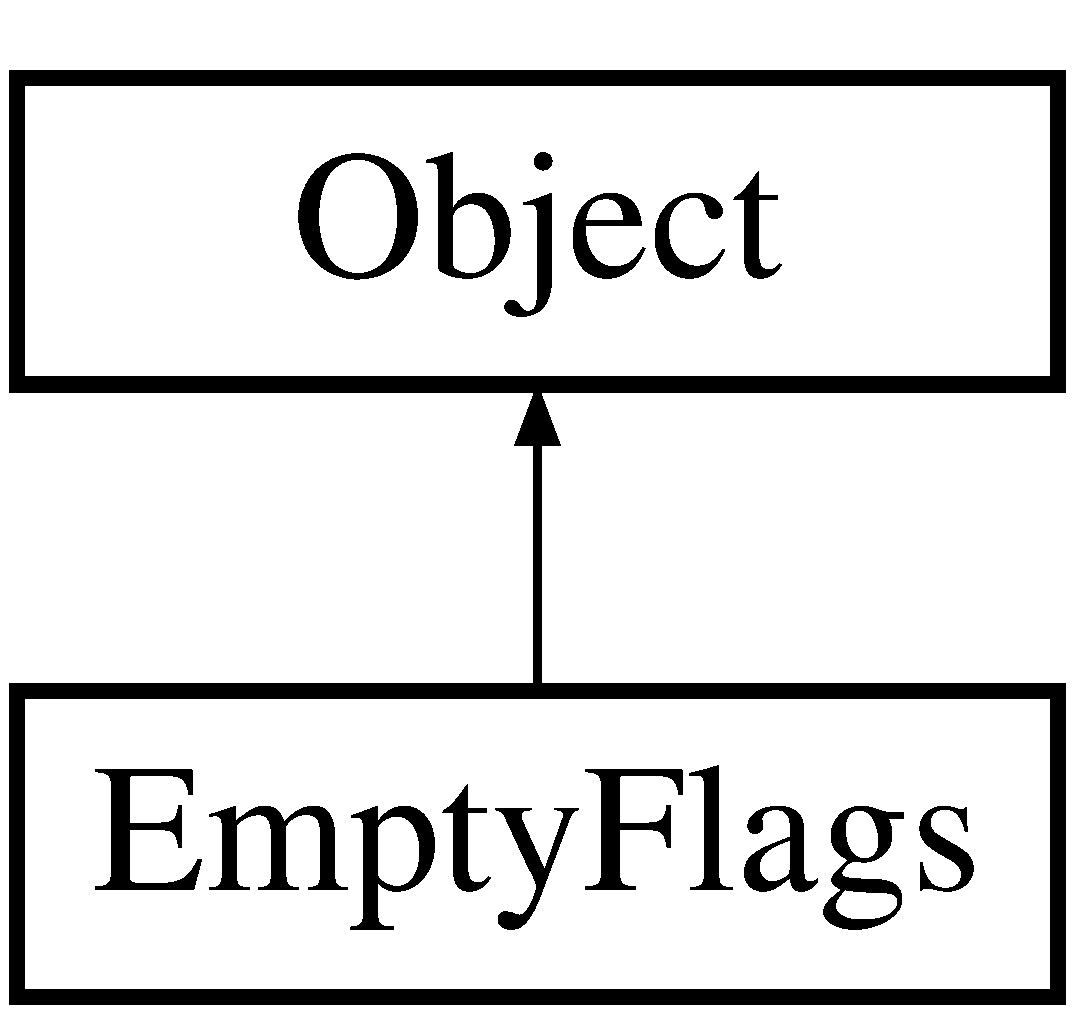
\includegraphics[height=2.000000cm]{structEmptyFlags}
\end{center}
\end{figure}


The documentation for this struct was generated from the following file\+:\begin{DoxyCompactItemize}
\item 
/home/pavel/projects/astro/sph2/src/structs/flags.\+h\end{DoxyCompactItemize}

\hypertarget{classAbstract_1_1Eos}{}\section{Abstract\+:\+:Eos Class Reference}
\label{classAbstract_1_1Eos}\index{Abstract\+::\+Eos@{Abstract\+::\+Eos}}


Base class for equations of state.  




{\ttfamily \#include $<$eos.\+h$>$}

Inheritance diagram for Abstract\+:\+:Eos\+:\begin{figure}[H]
\begin{center}
\leavevmode
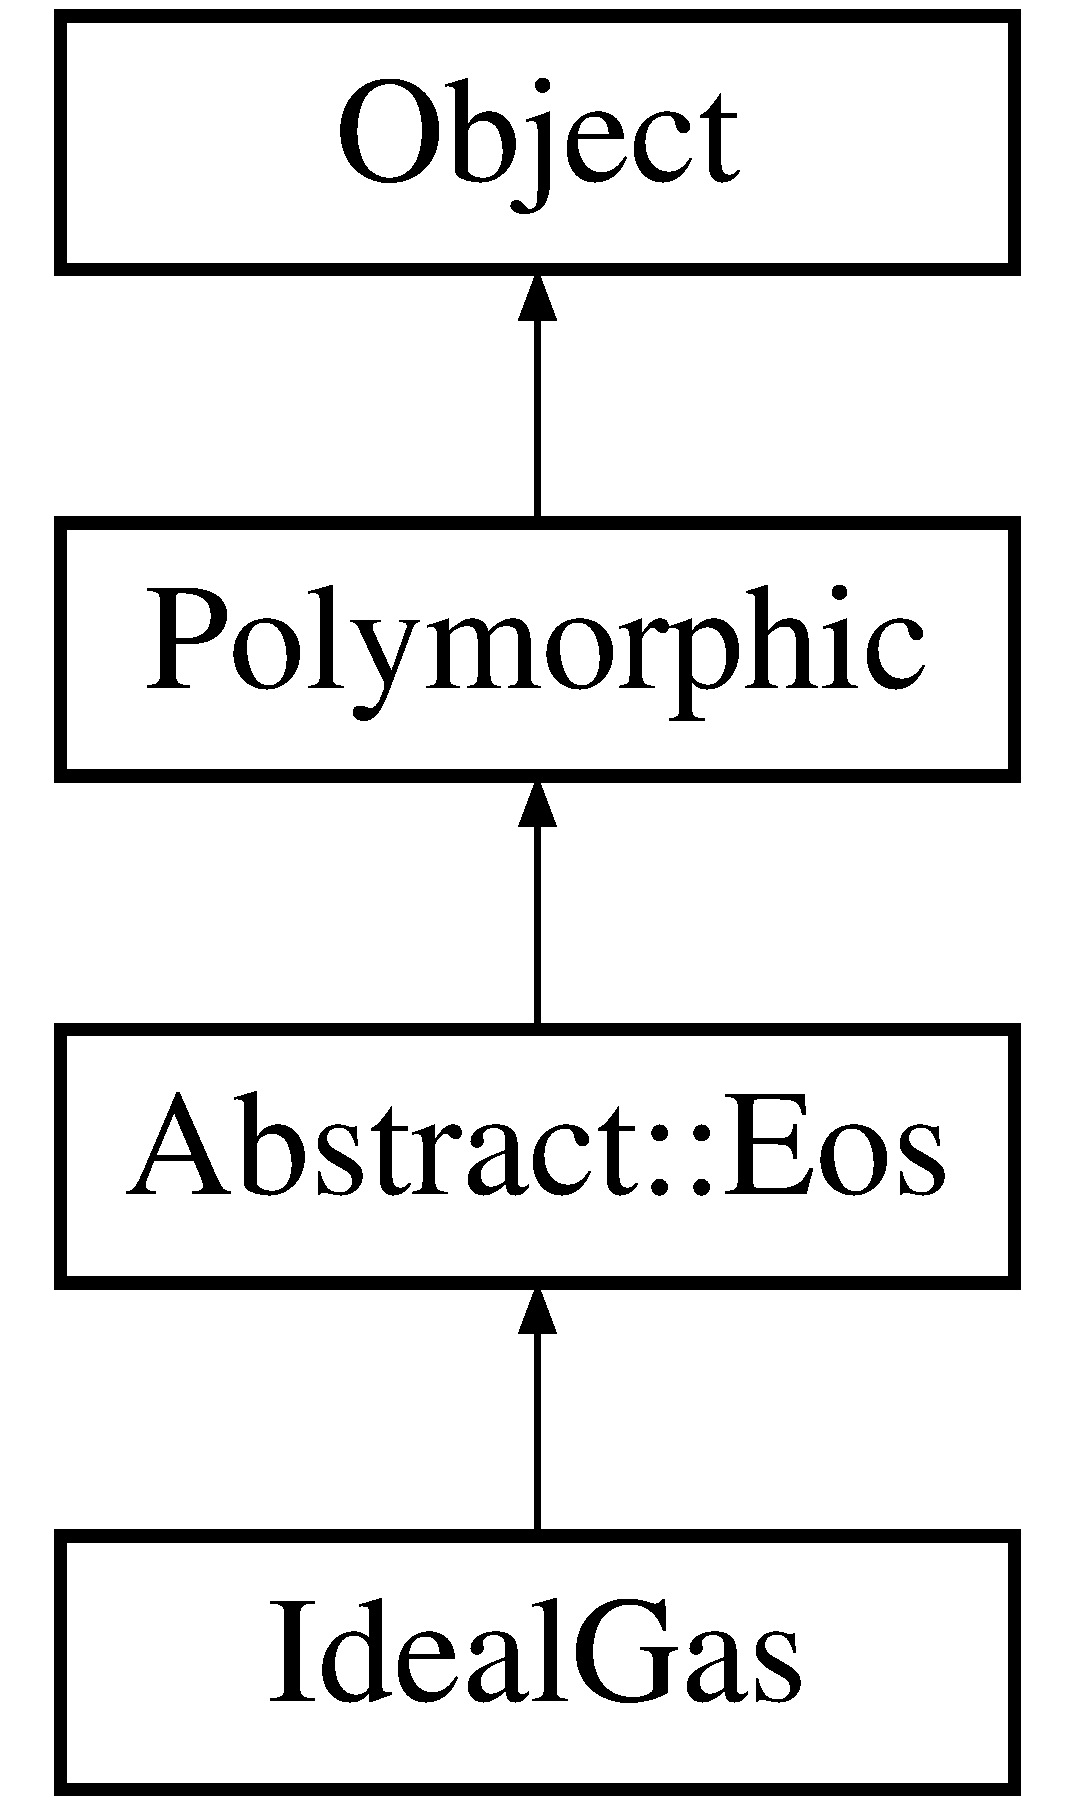
\includegraphics[height=4.000000cm]{classAbstract_1_1Eos}
\end{center}
\end{figure}
\subsection*{Public Member Functions}
\begin{DoxyCompactItemize}
\item 
virtual void \hyperlink{classAbstract_1_1Eos_ab21906f5fc78370a10cdbf97983544ea}{get\+Pressure} (\hyperlink{classArrayView}{Array\+View}$<$ const Float $>$ rho, \hyperlink{classArrayView}{Array\+View}$<$ const Float $>$ u, \hyperlink{classArrayView}{Array\+View}$<$ Float $>$ p)=0
\end{DoxyCompactItemize}


\subsection{Detailed Description}
Base class for equations of state. 

\subsection{Member Function Documentation}
\hypertarget{classAbstract_1_1Eos_ab21906f5fc78370a10cdbf97983544ea}{}\label{classAbstract_1_1Eos_ab21906f5fc78370a10cdbf97983544ea} 
\index{Abstract\+::\+Eos@{Abstract\+::\+Eos}!get\+Pressure@{get\+Pressure}}
\index{get\+Pressure@{get\+Pressure}!Abstract\+::\+Eos@{Abstract\+::\+Eos}}
\subsubsection{\texorpdfstring{get\+Pressure()}{getPressure()}}
{\footnotesize\ttfamily virtual void Abstract\+::\+Eos\+::get\+Pressure (\begin{DoxyParamCaption}\item[{\hyperlink{classArrayView}{Array\+View}$<$ const Float $>$}]{rho,  }\item[{\hyperlink{classArrayView}{Array\+View}$<$ const Float $>$}]{u,  }\item[{\hyperlink{classArrayView}{Array\+View}$<$ Float $>$}]{p }\end{DoxyParamCaption})\hspace{0.3cm}{\ttfamily [pure virtual]}}

Computes a pressure from given density. \begin{DoxyRefDesc}{Todo}
\item[\hyperlink{todo__todo000018}{Todo}]EoS have more general relations, like P = P(rho, T) or P = P(rho, u) 

maybe pass model as a parameter? \end{DoxyRefDesc}


Implemented in \hyperlink{classIdealGas_a27ee0a167bbb7e5690ce6db5fca39ba1}{Ideal\+Gas}.



The documentation for this class was generated from the following file\+:\begin{DoxyCompactItemize}
\item 
/home/pavel/projects/astro/sph2/src/physics/eos.\+h\end{DoxyCompactItemize}

\hypertarget{structEps}{}\section{Eps$<$ T $>$ Struct Template Reference}
\label{structEps}\index{Eps$<$ T $>$@{Eps$<$ T $>$}}


Small value (compared with 1) for given precision.  




{\ttfamily \#include $<$math.\+h$>$}



\subsection{Detailed Description}
\subsubsection*{template$<$typename T$>$\newline
struct Eps$<$ T $>$}

Small value (compared with 1) for given precision. 

The documentation for this struct was generated from the following file\+:\begin{DoxyCompactItemize}
\item 
/home/pavel/projects/astro/sph2/src/core/math.\+h\end{DoxyCompactItemize}

\hypertarget{structEps_3_01double_01_4}{}\section{Eps$<$ double $>$ Struct Template Reference}
\label{structEps_3_01double_01_4}\index{Eps$<$ double $>$@{Eps$<$ double $>$}}
\subsection*{Static Public Attributes}
\begin{DoxyCompactItemize}
\item 
\hypertarget{structEps_3_01double_01_4_a7a709ddb2d2883b9ee8e0fcf385cd3d3}{}\label{structEps_3_01double_01_4_a7a709ddb2d2883b9ee8e0fcf385cd3d3} 
static constexpr double {\bfseries value} = 1.e-\/12f
\end{DoxyCompactItemize}


The documentation for this struct was generated from the following file\+:\begin{DoxyCompactItemize}
\item 
/home/pavel/projects/astro/sph2/src/core/math.\+h\end{DoxyCompactItemize}

\hypertarget{structEps_3_01float_01_4}{}\section{Eps$<$ float $>$ Struct Template Reference}
\label{structEps_3_01float_01_4}\index{Eps$<$ float $>$@{Eps$<$ float $>$}}
\subsection*{Static Public Attributes}
\begin{DoxyCompactItemize}
\item 
\hypertarget{structEps_3_01float_01_4_aa6a3208f7af26cf57f0ad1362afeffcd}{}\label{structEps_3_01float_01_4_aa6a3208f7af26cf57f0ad1362afeffcd} 
static constexpr float {\bfseries value} = 1.e-\/6f
\end{DoxyCompactItemize}


The documentation for this struct was generated from the following file\+:\begin{DoxyCompactItemize}
\item 
/home/pavel/projects/astro/sph2/src/core/math.\+h\end{DoxyCompactItemize}

\hypertarget{classEulerExplicit}{}\section{Euler\+Explicit Class Reference}
\label{classEulerExplicit}\index{Euler\+Explicit@{Euler\+Explicit}}
Inheritance diagram for Euler\+Explicit\+:\begin{figure}[H]
\begin{center}
\leavevmode
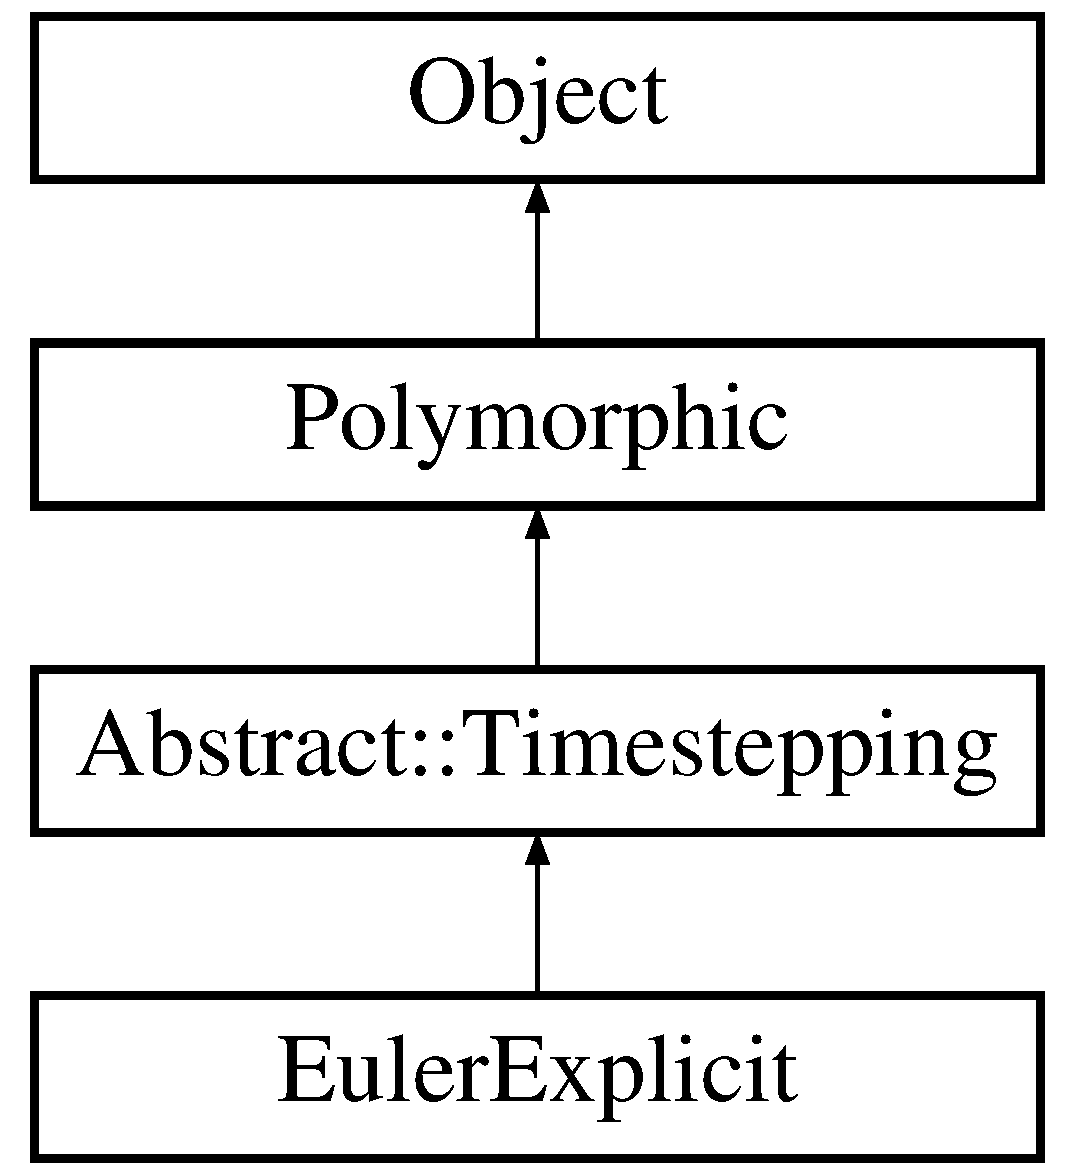
\includegraphics[height=4.000000cm]{classEulerExplicit}
\end{center}
\end{figure}
\subsection*{Public Member Functions}
\begin{DoxyCompactItemize}
\item 
\hypertarget{classEulerExplicit_ad0eb5290cc6b7d10ce961e7e489dea1a}{}\label{classEulerExplicit_ad0eb5290cc6b7d10ce961e7e489dea1a} 
{\bfseries Euler\+Explicit} (const Float timestep=0.\+\_\+f)
\end{DoxyCompactItemize}
\subsection*{Protected Member Functions}
\begin{DoxyCompactItemize}
\item 
\hypertarget{classEulerExplicit_a55222e61b1c3660a5722def70d817cbb}{}\label{classEulerExplicit_a55222e61b1c3660a5722def70d817cbb} 
virtual void {\bfseries step\+Scalar} (\hyperlink{classArray}{Array}$<$ Float $>$ \&array, const \hyperlink{classArray}{Array}$<$ Float $>$ \&deriv) override
\item 
\hypertarget{classEulerExplicit_a0141fd4bf38cd57e6e7ab26d4dc99aab}{}\label{classEulerExplicit_a0141fd4bf38cd57e6e7ab26d4dc99aab} 
virtual void {\bfseries step\+Vector} (\hyperlink{classArray}{Array}$<$ \hyperlink{classBasicVector}{Vector} $>$ \&array, const \hyperlink{classArray}{Array}$<$ \hyperlink{classBasicVector}{Vector} $>$ \&deriv) override
\end{DoxyCompactItemize}
\subsection*{Additional Inherited Members}


The documentation for this class was generated from the following file\+:\begin{DoxyCompactItemize}
\item 
/home/pavel/projects/astro/sph2/src/core/timestepping.\+h\end{DoxyCompactItemize}

\hypertarget{classFactory}{}\section{Factory Class Reference}
\label{classFactory}\index{Factory@{Factory}}


Class providing construction of objects from enums. Contain only static member functions.  




{\ttfamily \#include $<$factory.\+h$>$}

Inheritance diagram for Factory\+:\begin{figure}[H]
\begin{center}
\leavevmode
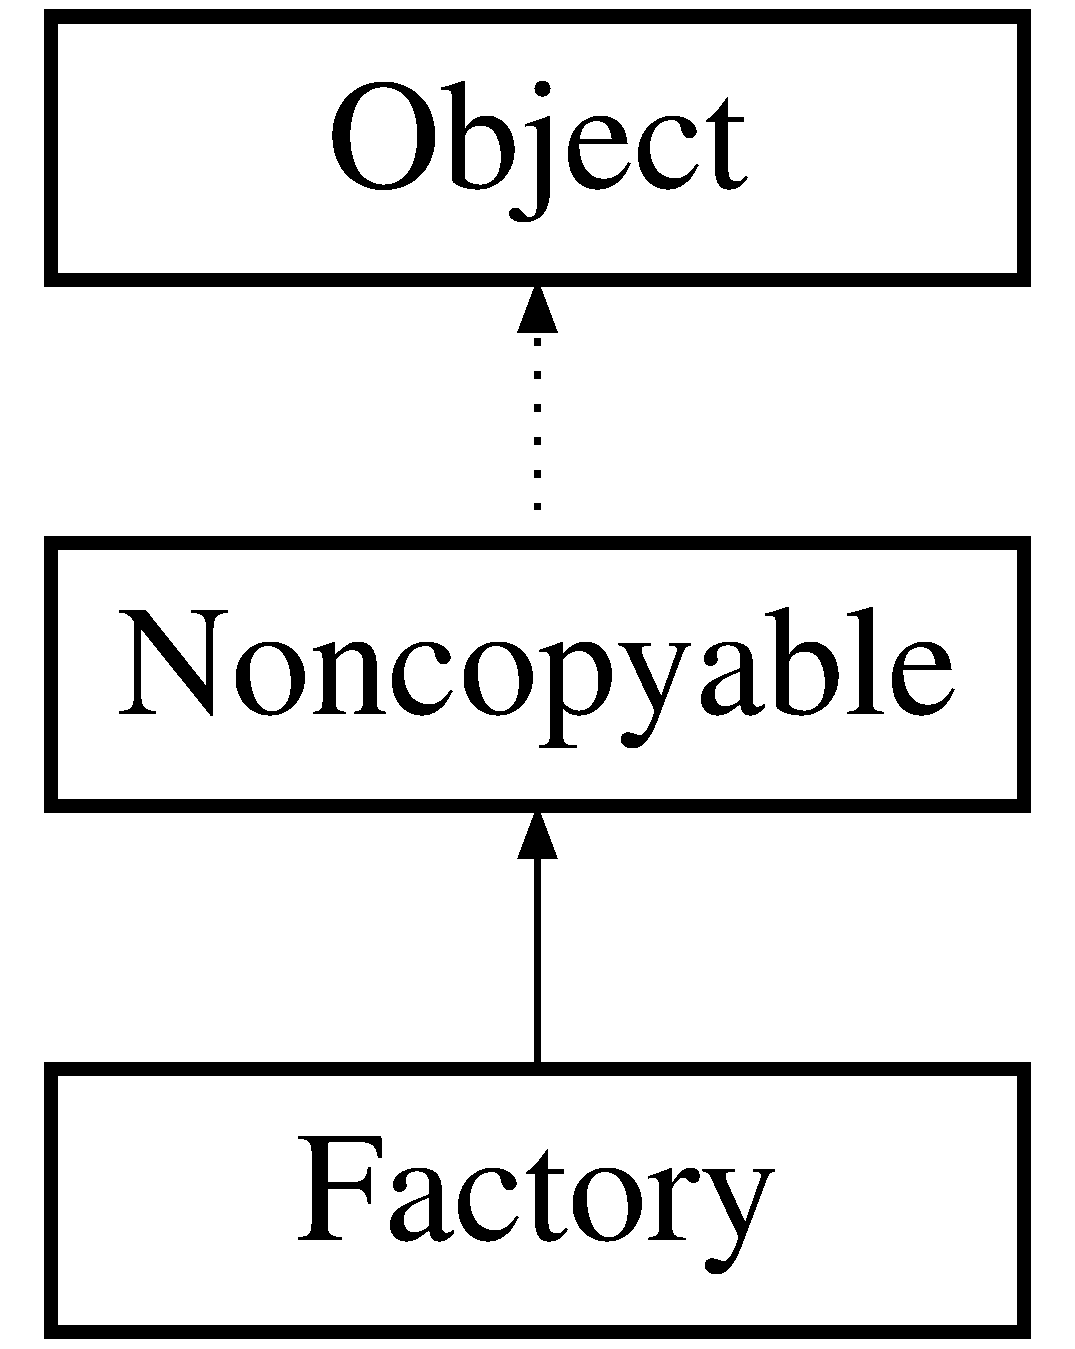
\includegraphics[height=3.000000cm]{classFactory}
\end{center}
\end{figure}
\subsection*{Static Public Member Functions}
\begin{DoxyCompactItemize}
\item 
\hypertarget{classFactory_a5a3f36d2925b0a78fecc385f391f9580}{}\label{classFactory_a5a3f36d2925b0a78fecc385f391f9580} 
static std\+::unique\+\_\+ptr$<$ \hyperlink{classAbstract_1_1Eos}{Abstract\+::\+Eos} $>$ {\bfseries get\+Eos} (const Eos\+Enum id)
\item 
\hypertarget{classFactory_a943bdf4efc1893c8ed68222a67e485ed}{}\label{classFactory_a943bdf4efc1893c8ed68222a67e485ed} 
static std\+::unique\+\_\+ptr$<$ \hyperlink{classAbstract_1_1Timestepping}{Abstract\+::\+Timestepping} $>$ {\bfseries get\+Timestepping} (const Timestepping\+Enum id)
\end{DoxyCompactItemize}
\subsection*{Additional Inherited Members}


\subsection{Detailed Description}
Class providing construction of objects from enums. Contain only static member functions. 

The documentation for this class was generated from the following files\+:\begin{DoxyCompactItemize}
\item 
/home/pavel/projects/astro/sph2/src/system/factory.\+h\item 
/home/pavel/projects/astro/sph2/src/system/factory.\+cpp\end{DoxyCompactItemize}

\hypertarget{classAbstract_1_1Finder}{}\section{Abstract\+:\+:Finder Class Reference}
\label{classAbstract_1_1Finder}\index{Abstract\+::\+Finder@{Abstract\+::\+Finder}}
Inheritance diagram for Abstract\+:\+:Finder\+:\begin{figure}[H]
\begin{center}
\leavevmode
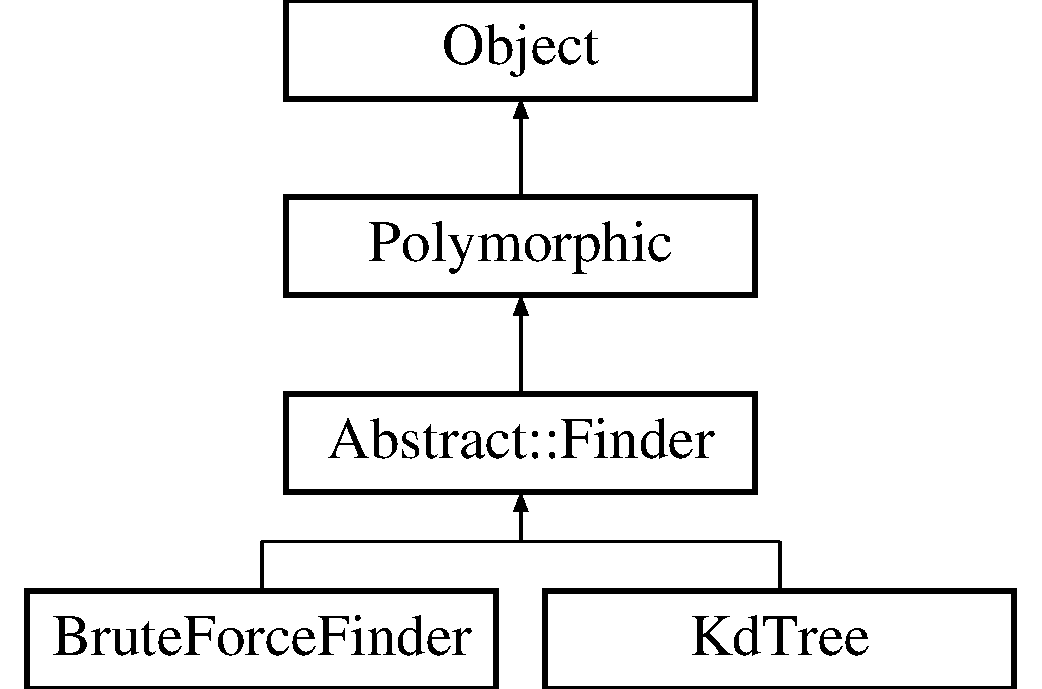
\includegraphics[height=4.000000cm]{classAbstract_1_1Finder}
\end{center}
\end{figure}
\subsection*{Public Member Functions}
\begin{DoxyCompactItemize}
\item 
\hypertarget{classAbstract_1_1Finder_a3a5ca4ed2bea8386862d3f3837077e0b}{}\label{classAbstract_1_1Finder_a3a5ca4ed2bea8386862d3f3837077e0b} 
void \hyperlink{classAbstract_1_1Finder_a3a5ca4ed2bea8386862d3f3837077e0b}{build} (\hyperlink{classArrayView}{Array\+View}$<$ \hyperlink{classBasicVector}{Vector} $>$ values)
\begin{DoxyCompactList}\small\item\em Constructs the struct with an array of vectors. \end{DoxyCompactList}\item 
virtual int \hyperlink{classAbstract_1_1Finder_a7f04b92d939992d0aa2978a259b2533f}{find\+Neighbours} (const int index, const Float radius, \hyperlink{classArray}{Array}$<$ \hyperlink{structNeighbourRecord}{Neighbour\+Record} $>$ \&neighbours, \hyperlink{classFlags}{Flags}$<$ Finder\+Flags $>$ flags=E\+M\+P\+T\+Y\+\_\+\+F\+L\+A\+GS, const Float error=0.\+\_\+f) const =0
\item 
\hypertarget{classAbstract_1_1Finder_a011e1092af4b447acd6bc4732e690b32}{}\label{classAbstract_1_1Finder_a011e1092af4b447acd6bc4732e690b32} 
virtual void \hyperlink{classAbstract_1_1Finder_a011e1092af4b447acd6bc4732e690b32}{rebuild} ()
\begin{DoxyCompactList}\small\item\em Updates the structure when the position change. \end{DoxyCompactList}\end{DoxyCompactItemize}
\subsection*{Protected Member Functions}
\begin{DoxyCompactItemize}
\item 
\hypertarget{classAbstract_1_1Finder_a77e7ccb5cbfb025f77962e18981a5718}{}\label{classAbstract_1_1Finder_a77e7ccb5cbfb025f77962e18981a5718} 
virtual void {\bfseries build\+Impl} (\hyperlink{classArrayView}{Array\+View}$<$ \hyperlink{classBasicVector}{Vector} $>$ values)=0
\end{DoxyCompactItemize}
\subsection*{Protected Attributes}
\begin{DoxyCompactItemize}
\item 
\hypertarget{classAbstract_1_1Finder_a5bba60f9a6bafcea0f014a31516f9b33}{}\label{classAbstract_1_1Finder_a5bba60f9a6bafcea0f014a31516f9b33} 
\hyperlink{classArrayView}{Array\+View}$<$ \hyperlink{classBasicVector}{Vector} $>$ {\bfseries values}
\item 
\hypertarget{classAbstract_1_1Finder_a5fc028a6ca9d4a46569076de2fe220a2}{}\label{classAbstract_1_1Finder_a5fc028a6ca9d4a46569076de2fe220a2} 
\hyperlink{classOrder}{Order} {\bfseries rankH}
\end{DoxyCompactItemize}


\subsection{Member Function Documentation}
\hypertarget{classAbstract_1_1Finder_a7f04b92d939992d0aa2978a259b2533f}{}\label{classAbstract_1_1Finder_a7f04b92d939992d0aa2978a259b2533f} 
\index{Abstract\+::\+Finder@{Abstract\+::\+Finder}!find\+Neighbours@{find\+Neighbours}}
\index{find\+Neighbours@{find\+Neighbours}!Abstract\+::\+Finder@{Abstract\+::\+Finder}}
\subsubsection{\texorpdfstring{find\+Neighbours()}{findNeighbours()}}
{\footnotesize\ttfamily virtual int Abstract\+::\+Finder\+::find\+Neighbours (\begin{DoxyParamCaption}\item[{const int}]{index,  }\item[{const Float}]{radius,  }\item[{\hyperlink{classArray}{Array}$<$ \hyperlink{structNeighbourRecord}{Neighbour\+Record} $>$ \&}]{neighbours,  }\item[{\hyperlink{classFlags}{Flags}$<$ Finder\+Flags $>$}]{flags = {\ttfamily EMPTY\+\_\+FLAGS},  }\item[{const Float}]{error = {\ttfamily 0.\+\_\+f} }\end{DoxyParamCaption}) const\hspace{0.3cm}{\ttfamily [pure virtual]}}

Finds all points within given radius from a point. 
\begin{DoxyParams}{Parameters}
{\em point} & \\
\hline
{\em radius} & \\
\hline
{\em neighbours} & List of neighbours, as indices to the array \\
\hline
{\em error} & Approximate solution \\
\hline
\end{DoxyParams}
\begin{DoxyReturn}{Returns}
The number of neighbours. 
\end{DoxyReturn}


Implemented in \hyperlink{classKdTree_a830840ce00b519f37e922a69733b68c1}{Kd\+Tree}.



The documentation for this class was generated from the following file\+:\begin{DoxyCompactItemize}
\item 
/home/pavel/projects/astro/sph2/src/tree/finder.\+h\end{DoxyCompactItemize}

\hypertarget{classFlags}{}\section{Flags$<$ T\+Enum $>$ Class Template Reference}
\label{classFlags}\index{Flags$<$ T\+Enum $>$@{Flags$<$ T\+Enum $>$}}
Inheritance diagram for Flags$<$ T\+Enum $>$\+:\begin{figure}[H]
\begin{center}
\leavevmode
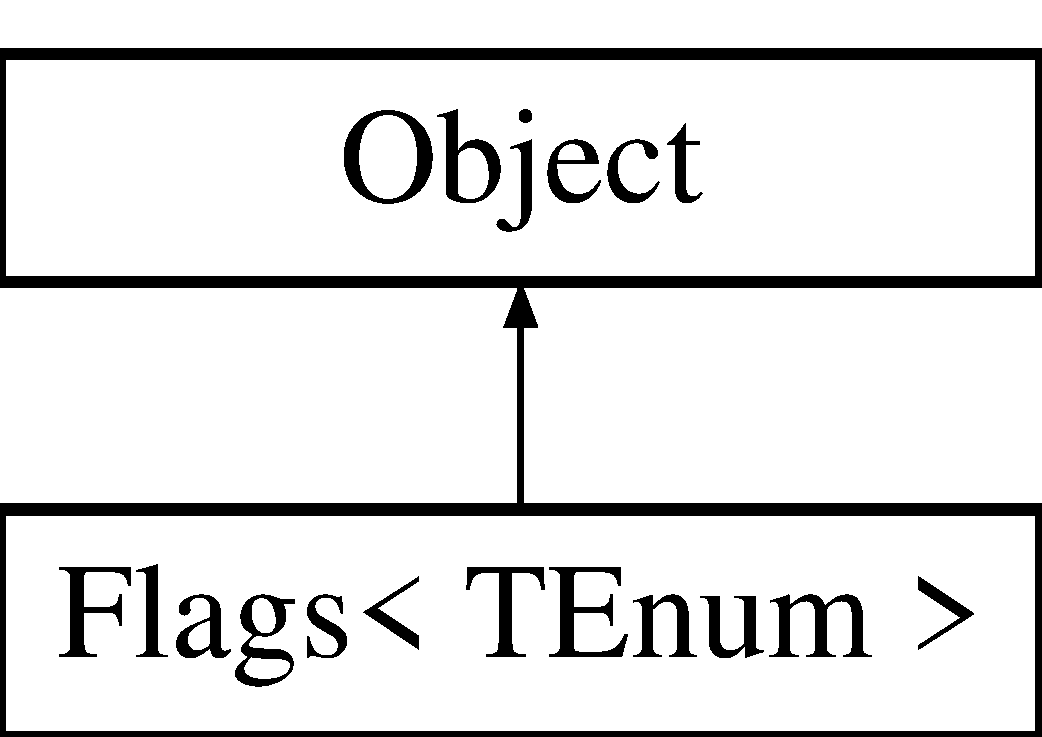
\includegraphics[height=2.000000cm]{classFlags}
\end{center}
\end{figure}
\subsection*{Public Member Functions}
\begin{DoxyCompactItemize}
\item 
\hypertarget{classFlags_aaaea7c330f4ffaa266da7424fe137bf3}{}\label{classFlags_aaaea7c330f4ffaa266da7424fe137bf3} 
constexpr {\bfseries Flags} (const \hyperlink{classFlags}{Flags} \&other)
\item 
\hypertarget{classFlags_a67682a31b1a6dd3b48380f66018f1967}{}\label{classFlags_a67682a31b1a6dd3b48380f66018f1967} 
constexpr {\bfseries Flags} (const T\+Enum \&flag)
\item 
\hypertarget{classFlags_a02d1646c04516dcbd5143fb227f8cc6f}{}\label{classFlags_a02d1646c04516dcbd5143fb227f8cc6f} 
constexpr {\bfseries Flags} (const \hyperlink{structEmptyFlags}{Empty\+Flags} \&)
\item 
\hypertarget{classFlags_a31303f5a1720ea7f5e8f0596153043f6}{}\label{classFlags_a31303f5a1720ea7f5e8f0596153043f6} 
\hyperlink{classFlags}{Flags} \& {\bfseries operator=} (const \hyperlink{classFlags}{Flags} \&other)
\item 
\hypertarget{classFlags_a3a8dea91e73fcbe35ec69b25f188cba4}{}\label{classFlags_a3a8dea91e73fcbe35ec69b25f188cba4} 
\hyperlink{classFlags}{Flags} \& {\bfseries operator=} (const T\+Enum \&flag)
\item 
\hypertarget{classFlags_a92eee8c71a46d2898b4d23543bfa5c69}{}\label{classFlags_a92eee8c71a46d2898b4d23543bfa5c69} 
\hyperlink{classFlags}{Flags} \& {\bfseries operator=} (const \hyperlink{structEmptyFlags}{Empty\+Flags} \&)
\item 
\hypertarget{classFlags_a03310032017d554f592f4652a97880c7}{}\label{classFlags_a03310032017d554f592f4652a97880c7} 
I\+N\+L\+I\+NE constexpr bool {\bfseries has} (const T\+Enum \&flag)
\item 
\hypertarget{classFlags_afa774f872964f72be8c2d847a9bdd659}{}\label{classFlags_afa774f872964f72be8c2d847a9bdd659} 
I\+N\+L\+I\+NE void {\bfseries set} (const T\+Enum \&flag)
\end{DoxyCompactItemize}


The documentation for this class was generated from the following file\+:\begin{DoxyCompactItemize}
\item 
/home/pavel/projects/astro/sph2/src/structs/flags.\+h\end{DoxyCompactItemize}

\hypertarget{structForCurrentType}{}\section{For\+Current\+Type$<$ n, T0, T\+Args $>$ Struct Template Reference}
\label{structForCurrentType}\index{For\+Current\+Type$<$ n, T0, T\+Args $>$@{For\+Current\+Type$<$ n, T0, T\+Args $>$}}


Executes a functor with the current value (and current type) as a parameter.  




{\ttfamily \#include $<$variant.\+h$>$}

\subsection*{Static Public Member Functions}
\begin{DoxyCompactItemize}
\item 
\hypertarget{structForCurrentType_ad6adf27f49de5abd55e84ea9ad5186f6}{}\label{structForCurrentType_ad6adf27f49de5abd55e84ea9ad5186f6} 
{\footnotesize template$<$typename T\+Functor $>$ }\\static void {\bfseries action} (const int idx, const char $\ast$data, T\+Functor \&\&functor)
\item 
\hypertarget{structForCurrentType_af3b60c9ad8e184b3609f08b2f77bd503}{}\label{structForCurrentType_af3b60c9ad8e184b3609f08b2f77bd503} 
{\footnotesize template$<$typename T\+Functor $>$ }\\static void {\bfseries action} (const int idx, char $\ast$data, T\+Functor \&\&functor)
\item 
\hypertarget{structForCurrentType_ad6adf27f49de5abd55e84ea9ad5186f6}{}\label{structForCurrentType_ad6adf27f49de5abd55e84ea9ad5186f6} 
{\footnotesize template$<$typename T\+Functor $>$ }\\static void {\bfseries action} (const int idx, const char $\ast$data, T\+Functor \&\&functor)
\item 
\hypertarget{structForCurrentType_af3b60c9ad8e184b3609f08b2f77bd503}{}\label{structForCurrentType_af3b60c9ad8e184b3609f08b2f77bd503} 
{\footnotesize template$<$typename T\+Functor $>$ }\\static void {\bfseries action} (const int idx, char $\ast$data, T\+Functor \&\&functor)
\end{DoxyCompactItemize}


\subsection{Detailed Description}
\subsubsection*{template$<$int n, typename T0, typename... T\+Args$>$\newline
struct For\+Current\+Type$<$ n, T0, T\+Args $>$}

Executes a functor with the current value (and current type) as a parameter. 

The documentation for this struct was generated from the following files\+:\begin{DoxyCompactItemize}
\item 
/home/pavel/projects/astro/sph2/src/structs/variant.\+h\item 
/home/pavel/projects/astro/sph2/src/structs/variant.\+old.\+h\end{DoxyCompactItemize}

\hypertarget{structForCurrentType_3_01n_00_01T0_01_4}{}\section{For\+Current\+Type$<$ n, T0 $>$ Struct Template Reference}
\label{structForCurrentType_3_01n_00_01T0_01_4}\index{For\+Current\+Type$<$ n, T0 $>$@{For\+Current\+Type$<$ n, T0 $>$}}
\subsection*{Static Public Member Functions}
\begin{DoxyCompactItemize}
\item 
\hypertarget{structForCurrentType_3_01n_00_01T0_01_4_a0fb2ea6a4934702bbe55ccf4d7395af8}{}\label{structForCurrentType_3_01n_00_01T0_01_4_a0fb2ea6a4934702bbe55ccf4d7395af8} 
{\footnotesize template$<$typename T\+Functor $>$ }\\static void {\bfseries action} (const int idx, const char $\ast$data, T\+Functor \&\&functor)
\item 
\hypertarget{structForCurrentType_3_01n_00_01T0_01_4_ab79902edf58340594116af09d4299bf7}{}\label{structForCurrentType_3_01n_00_01T0_01_4_ab79902edf58340594116af09d4299bf7} 
{\footnotesize template$<$typename T\+Functor $>$ }\\static void {\bfseries action} (const int idx, char $\ast$data, T\+Functor \&\&functor)
\item 
\hypertarget{structForCurrentType_3_01n_00_01T0_01_4_a0fb2ea6a4934702bbe55ccf4d7395af8}{}\label{structForCurrentType_3_01n_00_01T0_01_4_a0fb2ea6a4934702bbe55ccf4d7395af8} 
{\footnotesize template$<$typename T\+Functor $>$ }\\static void {\bfseries action} (const int idx, const char $\ast$data, T\+Functor \&\&functor)
\item 
\hypertarget{structForCurrentType_3_01n_00_01T0_01_4_ab79902edf58340594116af09d4299bf7}{}\label{structForCurrentType_3_01n_00_01T0_01_4_ab79902edf58340594116af09d4299bf7} 
{\footnotesize template$<$typename T\+Functor $>$ }\\static void {\bfseries action} (const int idx, char $\ast$data, T\+Functor \&\&functor)
\end{DoxyCompactItemize}


The documentation for this struct was generated from the following files\+:\begin{DoxyCompactItemize}
\item 
/home/pavel/projects/astro/sph2/src/structs/variant.\+h\item 
/home/pavel/projects/astro/sph2/src/structs/variant.\+old.\+h\end{DoxyCompactItemize}

\hypertarget{structforEachImpl}{}\section{for\+Each\+Impl$<$ i, n, T\+Functor, T\+Args $>$ Struct Template Reference}
\label{structforEachImpl}\index{for\+Each\+Impl$<$ i, n, T\+Functor, T\+Args $>$@{for\+Each\+Impl$<$ i, n, T\+Functor, T\+Args $>$}}


{\ttfamily \#include $<$tuple.\+h$>$}

Inheritance diagram for for\+Each\+Impl$<$ i, n, T\+Functor, T\+Args $>$\+:\begin{figure}[H]
\begin{center}
\leavevmode
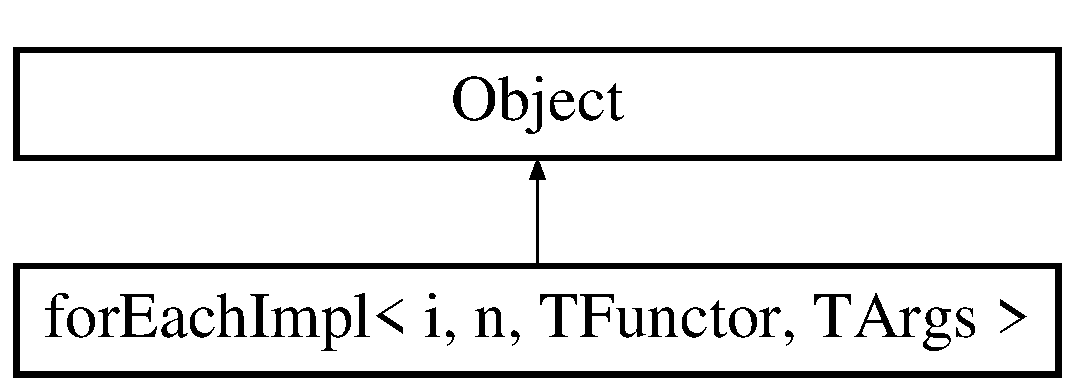
\includegraphics[height=2.000000cm]{structforEachImpl}
\end{center}
\end{figure}
\subsection*{Static Public Member Functions}
\begin{DoxyCompactItemize}
\item 
\hypertarget{structforEachImpl_a30c25aa31f9b359a35a8f0352977bd10}{}\label{structforEachImpl_a30c25aa31f9b359a35a8f0352977bd10} 
static void {\bfseries action} (\hyperlink{classTuple}{Tuple}$<$ T\+Args... $>$ \&tuple, T\+Functor functor)
\item 
\hypertarget{structforEachImpl_a982d6b72789b6540046780db843bdfd1}{}\label{structforEachImpl_a982d6b72789b6540046780db843bdfd1} 
static void {\bfseries action} (const \hyperlink{classTuple}{Tuple}$<$ T\+Args... $>$ \&tuple, T\+Functor functor)
\end{DoxyCompactItemize}


\subsection{Detailed Description}
\subsubsection*{template$<$int i, int n, typename T\+Functor, typename... T\+Args$>$\newline
struct for\+Each\+Impl$<$ i, n, T\+Functor, T\+Args $>$}

for loop to iterate over tuple. The functor must be a generic lambda or have overloaded operators() for all types stored within tuple. 

The documentation for this struct was generated from the following file\+:\begin{DoxyCompactItemize}
\item 
/home/pavel/projects/astro/sph2/src/structs/tuple.\+h\end{DoxyCompactItemize}

\hypertarget{structforEachImpl_3_01n_00_01n_00_01TFunctor_00_01TArgs_8_8_8_01_4}{}\section{for\+Each\+Impl$<$ n, n, T\+Functor, T\+Args... $>$ Struct Template Reference}
\label{structforEachImpl_3_01n_00_01n_00_01TFunctor_00_01TArgs_8_8_8_01_4}\index{for\+Each\+Impl$<$ n, n, T\+Functor, T\+Args... $>$@{for\+Each\+Impl$<$ n, n, T\+Functor, T\+Args... $>$}}
Inheritance diagram for for\+Each\+Impl$<$ n, n, T\+Functor, T\+Args... $>$\+:\begin{figure}[H]
\begin{center}
\leavevmode
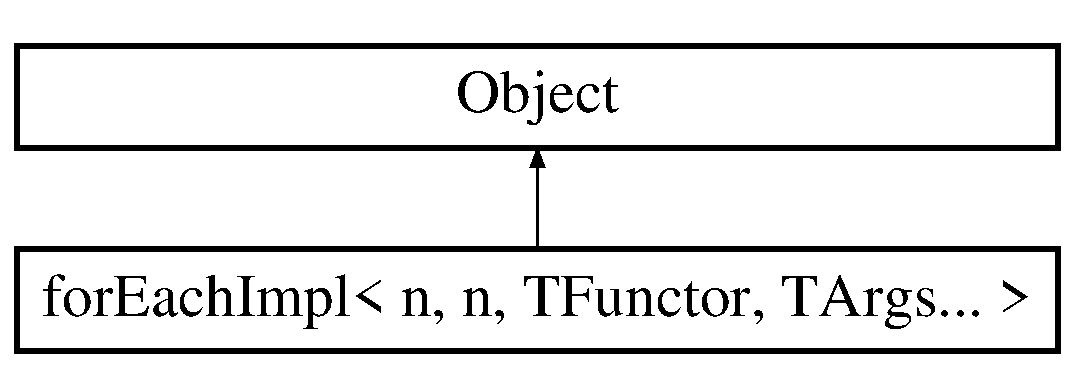
\includegraphics[height=2.000000cm]{structforEachImpl_3_01n_00_01n_00_01TFunctor_00_01TArgs_8_8_8_01_4}
\end{center}
\end{figure}
\subsection*{Static Public Member Functions}
\begin{DoxyCompactItemize}
\item 
\hypertarget{structforEachImpl_3_01n_00_01n_00_01TFunctor_00_01TArgs_8_8_8_01_4_a2395d2d4580cb7c405535eab23cc2006}{}\label{structforEachImpl_3_01n_00_01n_00_01TFunctor_00_01TArgs_8_8_8_01_4_a2395d2d4580cb7c405535eab23cc2006} 
static void {\bfseries action} (\hyperlink{classTuple}{Tuple}$<$ T\+Args... $>$ \&tuple, T\+Functor functor)
\item 
\hypertarget{structforEachImpl_3_01n_00_01n_00_01TFunctor_00_01TArgs_8_8_8_01_4_aeda3f0b218679fc916334d6933b6db46}{}\label{structforEachImpl_3_01n_00_01n_00_01TFunctor_00_01TArgs_8_8_8_01_4_aeda3f0b218679fc916334d6933b6db46} 
static void {\bfseries action} (const \hyperlink{classTuple}{Tuple}$<$ T\+Args... $>$ \&tuple, T\+Functor functor)
\end{DoxyCompactItemize}


The documentation for this struct was generated from the following file\+:\begin{DoxyCompactItemize}
\item 
/home/pavel/projects/astro/sph2/src/structs/tuple.\+h\end{DoxyCompactItemize}

\hypertarget{structFunctionSignature}{}\section{Function\+Signature$<$ T\+Signature $>$ Struct Template Reference}
\label{structFunctionSignature}\index{Function\+Signature$<$ T\+Signature $>$@{Function\+Signature$<$ T\+Signature $>$}}


Function traits.  




{\ttfamily \#include $<$traits.\+h$>$}

\subsection*{Public Types}
\begin{DoxyCompactItemize}
\item 
\hypertarget{structFunctionSignature_a06bbb69f569c95ae9adf739de896bc87}{}\label{structFunctionSignature_a06bbb69f569c95ae9adf739de896bc87} 
using {\bfseries T} = T\+Signature
\end{DoxyCompactItemize}


\subsection{Detailed Description}
\subsubsection*{template$<$typename T\+Signature$>$\newline
struct Function\+Signature$<$ T\+Signature $>$}

Function traits. 

The documentation for this struct was generated from the following file\+:\begin{DoxyCompactItemize}
\item 
/home/pavel/projects/astro/sph2/src/core/traits.\+h\end{DoxyCompactItemize}

\hypertarget{structFunctionTraits}{}\section{Function\+Traits$<$ T\+Function $>$ Struct Template Reference}
\label{structFunctionTraits}\index{Function\+Traits$<$ T\+Function $>$@{Function\+Traits$<$ T\+Function $>$}}
\subsection*{Public Types}
\begin{DoxyCompactItemize}
\item 
\hypertarget{structFunctionTraits_a58f8bd16cb255f7d796933ea76fe6f5c}{}\label{structFunctionTraits_a58f8bd16cb255f7d796933ea76fe6f5c} 
using {\bfseries T\+Signature} = typename \hyperlink{structFunctionTraits}{Function\+Traits}$<$ decltype(\&T\+Function\+::operator())$>$\+::T\+Signature
\end{DoxyCompactItemize}


The documentation for this struct was generated from the following file\+:\begin{DoxyCompactItemize}
\item 
/home/pavel/projects/astro/sph2/src/core/traits.\+h\end{DoxyCompactItemize}

\hypertarget{structFunctionTraits_3_01TReturn_07_5_08_07TArgs_8_8_8_08_4}{}\section{Function\+Traits$<$ T\+Return($\ast$)(T\+Args...)$>$ Struct Template Reference}
\label{structFunctionTraits_3_01TReturn_07_5_08_07TArgs_8_8_8_08_4}\index{Function\+Traits$<$ T\+Return($\ast$)(\+T\+Args...)$>$@{Function\+Traits$<$ T\+Return($\ast$)(\+T\+Args...)$>$}}
\subsection*{Public Types}
\begin{DoxyCompactItemize}
\item 
\hypertarget{structFunctionTraits_3_01TReturn_07_5_08_07TArgs_8_8_8_08_4_a181f96d12b95a0690481ba21b6b07a19}{}\label{structFunctionTraits_3_01TReturn_07_5_08_07TArgs_8_8_8_08_4_a181f96d12b95a0690481ba21b6b07a19} 
using {\bfseries T\+Signature} = typename \hyperlink{structFunctionSignature}{Function\+Signature}$<$ T\+Return(T\+Args...)$>$\+::T
\item 
\hypertarget{structFunctionTraits_3_01TReturn_07_5_08_07TArgs_8_8_8_08_4_a15302b4e0fa16b72dadc32f7f0e6d7ec}{}\label{structFunctionTraits_3_01TReturn_07_5_08_07TArgs_8_8_8_08_4_a15302b4e0fa16b72dadc32f7f0e6d7ec} 
using {\bfseries T\+Return\+Type} = T\+Return
\end{DoxyCompactItemize}


The documentation for this struct was generated from the following file\+:\begin{DoxyCompactItemize}
\item 
/home/pavel/projects/astro/sph2/src/core/traits.\+h\end{DoxyCompactItemize}

\hypertarget{structFunctionTraits_3_01TReturn_07TClass_1_1_5_08_07TArgs_8_8_8_08_01const_01_4}{}\section{Function\+Traits$<$ T\+Return(T\+Class\+:\+:$\ast$)(T\+Args...) const $>$ Struct Template Reference}
\label{structFunctionTraits_3_01TReturn_07TClass_1_1_5_08_07TArgs_8_8_8_08_01const_01_4}\index{Function\+Traits$<$ T\+Return(\+T\+Class\+::$\ast$)(\+T\+Args...) const $>$@{Function\+Traits$<$ T\+Return(\+T\+Class\+::$\ast$)(\+T\+Args...) const $>$}}
\subsection*{Public Types}
\begin{DoxyCompactItemize}
\item 
\hypertarget{structFunctionTraits_3_01TReturn_07TClass_1_1_5_08_07TArgs_8_8_8_08_01const_01_4_a0163b350a80b316c663b1a3c44c677cf}{}\label{structFunctionTraits_3_01TReturn_07TClass_1_1_5_08_07TArgs_8_8_8_08_01const_01_4_a0163b350a80b316c663b1a3c44c677cf} 
using {\bfseries T\+Signature} = typename \hyperlink{structFunctionSignature}{Function\+Signature}$<$ T\+Return(T\+Args...)$>$\+::T
\item 
\hypertarget{structFunctionTraits_3_01TReturn_07TClass_1_1_5_08_07TArgs_8_8_8_08_01const_01_4_aa39737a1566ded005a47ab3f18199229}{}\label{structFunctionTraits_3_01TReturn_07TClass_1_1_5_08_07TArgs_8_8_8_08_01const_01_4_aa39737a1566ded005a47ab3f18199229} 
using {\bfseries T\+Return\+Type} = T\+Return
\end{DoxyCompactItemize}


The documentation for this struct was generated from the following file\+:\begin{DoxyCompactItemize}
\item 
/home/pavel/projects/astro/sph2/src/core/traits.\+h\end{DoxyCompactItemize}

\hypertarget{structFunctionTraits_3_01TReturn_07TClass_1_1_5_08_07TArgs_8_8_8_08_4}{}\section{Function\+Traits$<$ T\+Return(T\+Class\+:\+:$\ast$)(T\+Args...)$>$ Struct Template Reference}
\label{structFunctionTraits_3_01TReturn_07TClass_1_1_5_08_07TArgs_8_8_8_08_4}\index{Function\+Traits$<$ T\+Return(\+T\+Class\+::$\ast$)(\+T\+Args...)$>$@{Function\+Traits$<$ T\+Return(\+T\+Class\+::$\ast$)(\+T\+Args...)$>$}}
\subsection*{Public Types}
\begin{DoxyCompactItemize}
\item 
\hypertarget{structFunctionTraits_3_01TReturn_07TClass_1_1_5_08_07TArgs_8_8_8_08_4_a85d9a0615c88aceb9940157567bfb5d9}{}\label{structFunctionTraits_3_01TReturn_07TClass_1_1_5_08_07TArgs_8_8_8_08_4_a85d9a0615c88aceb9940157567bfb5d9} 
using {\bfseries T\+Signature} = typename \hyperlink{structFunctionSignature}{Function\+Signature}$<$ T\+Return(T\+Args...)$>$\+::T
\item 
\hypertarget{structFunctionTraits_3_01TReturn_07TClass_1_1_5_08_07TArgs_8_8_8_08_4_afb75119740cff4ca49102552cf04bc8d}{}\label{structFunctionTraits_3_01TReturn_07TClass_1_1_5_08_07TArgs_8_8_8_08_4_afb75119740cff4ca49102552cf04bc8d} 
using {\bfseries T\+Return\+Type} = T\+Return
\end{DoxyCompactItemize}


The documentation for this struct was generated from the following file\+:\begin{DoxyCompactItemize}
\item 
/home/pavel/projects/astro/sph2/src/core/traits.\+h\end{DoxyCompactItemize}

\hypertarget{structGetMaxAlignmentType}{}\section{Get\+Max\+Alignment\+Type$<$ T\+Args $>$ Struct Template Reference}
\label{structGetMaxAlignmentType}\index{Get\+Max\+Alignment\+Type$<$ T\+Args $>$@{Get\+Max\+Alignment\+Type$<$ T\+Args $>$}}


{\ttfamily \#include $<$variant.\+old.\+h$>$}

Inheritance diagram for Get\+Max\+Alignment\+Type$<$ T\+Args $>$\+:\begin{figure}[H]
\begin{center}
\leavevmode
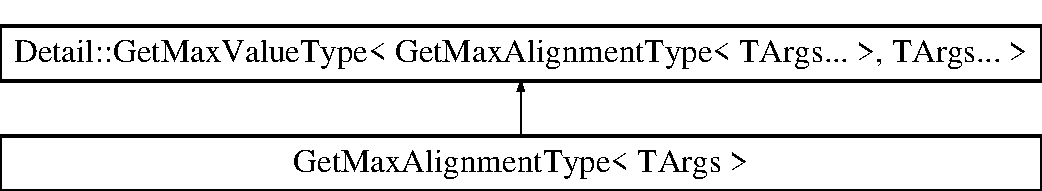
\includegraphics[height=2.000000cm]{structGetMaxAlignmentType}
\end{center}
\end{figure}
\subsection*{Static Public Member Functions}
\begin{DoxyCompactItemize}
\item 
\hypertarget{structGetMaxAlignmentType_a76eef930ca8b3e83a780881c578ec872}{}\label{structGetMaxAlignmentType_a76eef930ca8b3e83a780881c578ec872} 
{\footnotesize template$<$typename T $>$ }\\static constexpr int {\bfseries get} ()
\end{DoxyCompactItemize}


\subsection{Detailed Description}
\subsubsection*{template$<$typename... T\+Args$>$\newline
struct Get\+Max\+Alignment\+Type$<$ T\+Args $>$}

Gets maximum alignment of all types. Since alignments are always powers of 2, maximum alignment fulfills alignments of all types. 

The documentation for this struct was generated from the following file\+:\begin{DoxyCompactItemize}
\item 
/home/pavel/projects/astro/sph2/src/structs/variant.\+old.\+h\end{DoxyCompactItemize}

\hypertarget{structGetMaxSizeType}{}\section{Get\+Max\+Size\+Type$<$ T\+Args $>$ Struct Template Reference}
\label{structGetMaxSizeType}\index{Get\+Max\+Size\+Type$<$ T\+Args $>$@{Get\+Max\+Size\+Type$<$ T\+Args $>$}}


Get a size of the largest type.  




{\ttfamily \#include $<$variant.\+old.\+h$>$}

Inheritance diagram for Get\+Max\+Size\+Type$<$ T\+Args $>$\+:\begin{figure}[H]
\begin{center}
\leavevmode
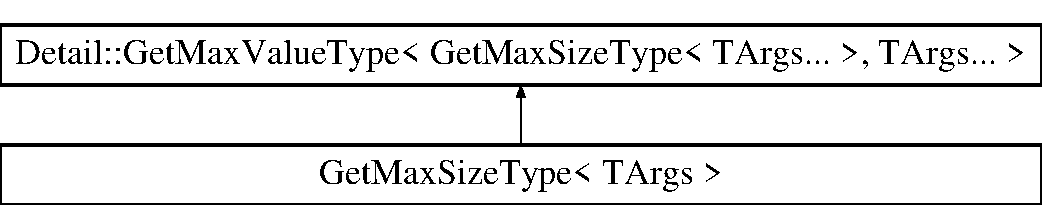
\includegraphics[height=2.000000cm]{structGetMaxSizeType}
\end{center}
\end{figure}
\subsection*{Static Public Member Functions}
\begin{DoxyCompactItemize}
\item 
\hypertarget{structGetMaxSizeType_a330706a7d04e2e87d72fadfe81a2629b}{}\label{structGetMaxSizeType_a330706a7d04e2e87d72fadfe81a2629b} 
{\footnotesize template$<$typename T $>$ }\\static constexpr int {\bfseries get} ()
\end{DoxyCompactItemize}


\subsection{Detailed Description}
\subsubsection*{template$<$typename... T\+Args$>$\newline
struct Get\+Max\+Size\+Type$<$ T\+Args $>$}

Get a size of the largest type. 

The documentation for this struct was generated from the following file\+:\begin{DoxyCompactItemize}
\item 
/home/pavel/projects/astro/sph2/src/structs/variant.\+old.\+h\end{DoxyCompactItemize}

\hypertarget{classGetTupleImplType}{}\section{Get\+Tuple\+Impl\+Type$<$ I, N, T0, T\+Args $>$ Class Template Reference}
\label{classGetTupleImplType}\index{Get\+Tuple\+Impl\+Type$<$ I, N, T0, T\+Args $>$@{Get\+Tuple\+Impl\+Type$<$ I, N, T0, T\+Args $>$}}


A helper type extracting the type of the n-\/th element.  




{\ttfamily \#include $<$tuple.\+h$>$}



\subsection{Detailed Description}
\subsubsection*{template$<$int I, int N, typename T0, typename... T\+Args$>$\newline
class Get\+Tuple\+Impl\+Type$<$ I, N, T0, T\+Args $>$}

A helper type extracting the type of the n-\/th element. 

The documentation for this class was generated from the following file\+:\begin{DoxyCompactItemize}
\item 
/home/pavel/projects/astro/sph2/src/structs/tuple.\+h\end{DoxyCompactItemize}

\hypertarget{classGetTupleImplType_3_01N_00_01N_00_01T0_00_01TArgs_8_8_8_01_4}{}\section{Get\+Tuple\+Impl\+Type$<$ N, N, T0, T\+Args... $>$ Class Template Reference}
\label{classGetTupleImplType_3_01N_00_01N_00_01T0_00_01TArgs_8_8_8_01_4}\index{Get\+Tuple\+Impl\+Type$<$ N, N, T0, T\+Args... $>$@{Get\+Tuple\+Impl\+Type$<$ N, N, T0, T\+Args... $>$}}
Inheritance diagram for Get\+Tuple\+Impl\+Type$<$ N, N, T0, T\+Args... $>$\+:\begin{figure}[H]
\begin{center}
\leavevmode
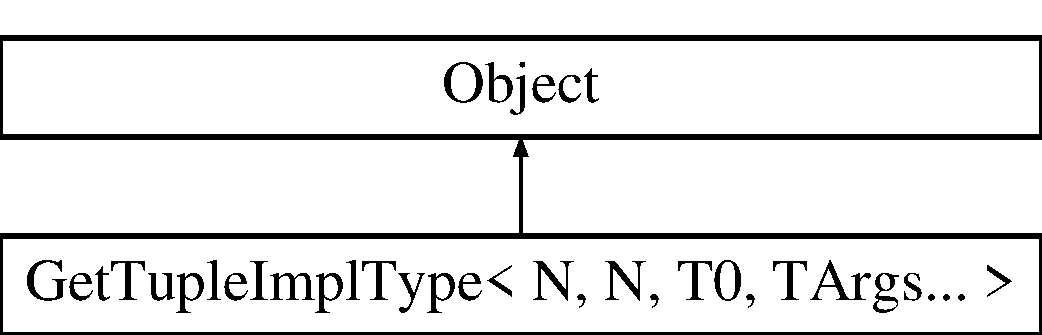
\includegraphics[height=2.000000cm]{classGetTupleImplType_3_01N_00_01N_00_01T0_00_01TArgs_8_8_8_01_4}
\end{center}
\end{figure}
\subsection*{Public Types}
\begin{DoxyCompactItemize}
\item 
\hypertarget{classGetTupleImplType_3_01N_00_01N_00_01T0_00_01TArgs_8_8_8_01_4_af6b3402d4e563daafe847e90ba20917f}{}\label{classGetTupleImplType_3_01N_00_01N_00_01T0_00_01TArgs_8_8_8_01_4_af6b3402d4e563daafe847e90ba20917f} 
using {\bfseries Type} = \hyperlink{classTupleImpl}{Tuple\+Impl}$<$ T0, T\+Args... $>$
\end{DoxyCompactItemize}


The documentation for this class was generated from the following file\+:\begin{DoxyCompactItemize}
\item 
/home/pavel/projects/astro/sph2/src/structs/tuple.\+h\end{DoxyCompactItemize}

\hypertarget{classHaltonQrng}{}\section{Halton\+Qrng Class Reference}
\label{classHaltonQrng}\index{Halton\+Qrng@{Halton\+Qrng}}


{\ttfamily \#include $<$rng.\+h$>$}

Inheritance diagram for Halton\+Qrng\+:\begin{figure}[H]
\begin{center}
\leavevmode
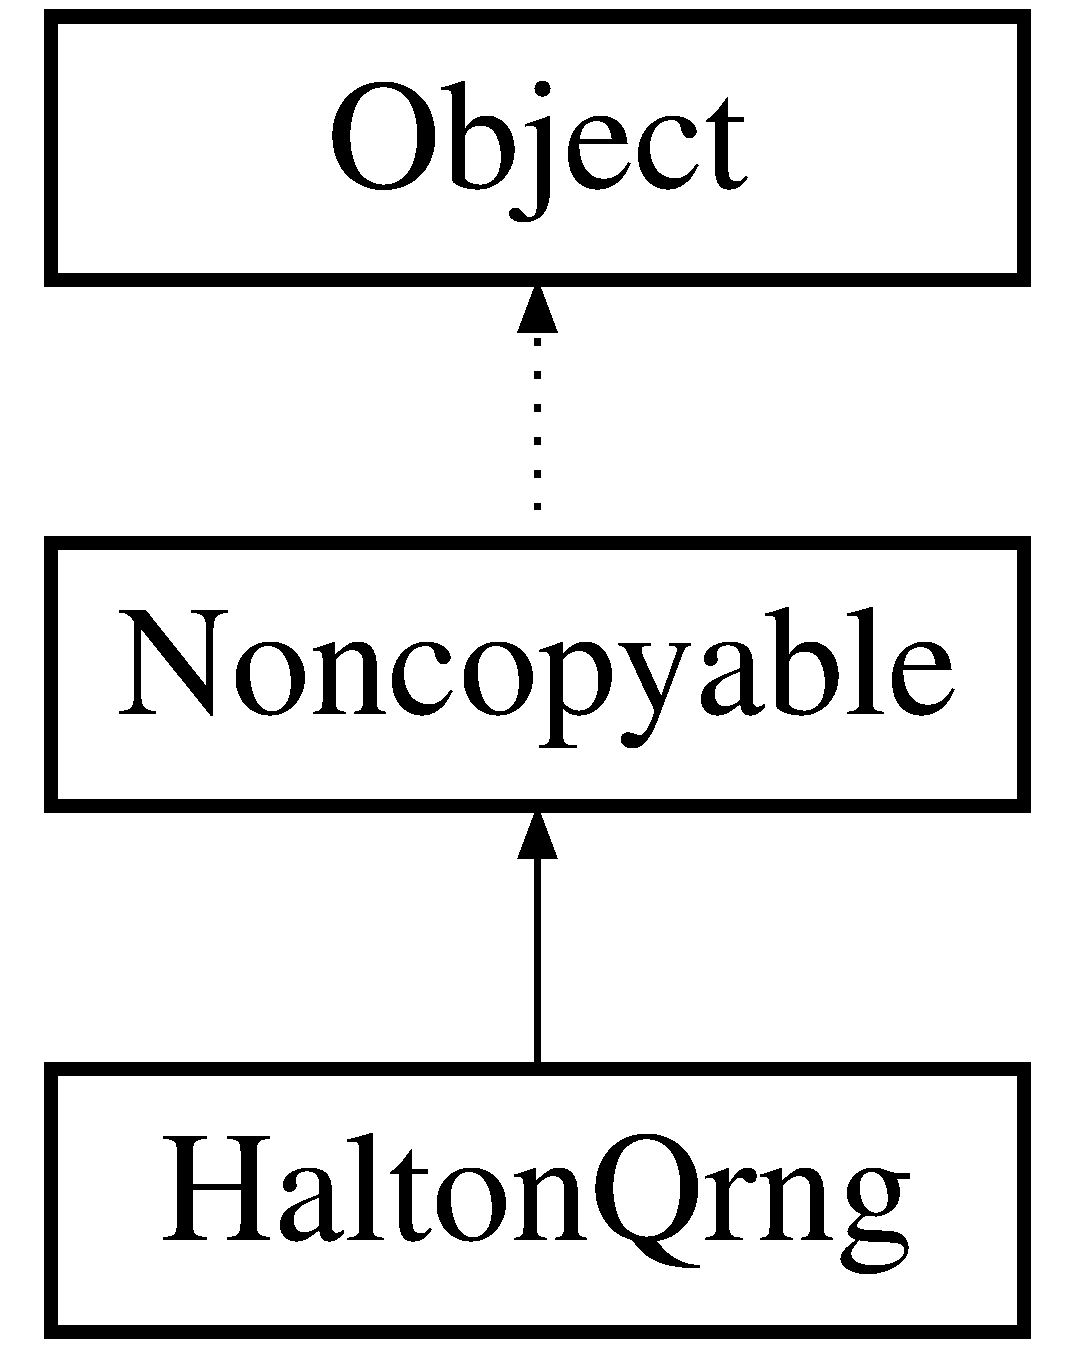
\includegraphics[height=3.000000cm]{classHaltonQrng}
\end{center}
\end{figure}
\subsection*{Public Member Functions}
\begin{DoxyCompactItemize}
\item 
\hypertarget{classHaltonQrng_a3b006ea9079cecf20883115fc384611e}{}\label{classHaltonQrng_a3b006ea9079cecf20883115fc384611e} 
{\bfseries Halton\+Qrng} (\hyperlink{classHaltonQrng}{Halton\+Qrng} \&\&other)
\item 
\hypertarget{classHaltonQrng_a8b3b37baa7e42890c350dadd9558d02a}{}\label{classHaltonQrng_a8b3b37baa7e42890c350dadd9558d02a} 
Float {\bfseries operator()} (const int s)
\end{DoxyCompactItemize}
\subsection*{Protected Member Functions}
\begin{DoxyCompactItemize}
\item 
\hypertarget{classHaltonQrng_aeb503898a8ea6da28c4c413e25d36b77}{}\label{classHaltonQrng_aeb503898a8ea6da28c4c413e25d36b77} 
Float {\bfseries radical\+Inverse} (const int base, int i)
\end{DoxyCompactItemize}
\subsection*{Protected Attributes}
\begin{DoxyCompactItemize}
\item 
\hypertarget{classHaltonQrng_a25fd783fa496c82588dc47b1bd13a21e}{}\label{classHaltonQrng_a25fd783fa496c82588dc47b1bd13a21e} 
\hyperlink{classStaticArray}{Static\+Array}$<$ int, dimension $>$ {\bfseries primes}
\item 
\hypertarget{classHaltonQrng_a553ba3536d92b86dc6b353ba04c1687f}{}\label{classHaltonQrng_a553ba3536d92b86dc6b353ba04c1687f} 
\hyperlink{classStaticArray}{Static\+Array}$<$ int, dimension $>$ {\bfseries c}
\end{DoxyCompactItemize}
\subsection*{Static Protected Attributes}
\begin{DoxyCompactItemize}
\item 
\hypertarget{classHaltonQrng_a9e1933d474c59dab416349fa32d9deb6}{}\label{classHaltonQrng_a9e1933d474c59dab416349fa32d9deb6} 
static const int {\bfseries dimension} = 6
\end{DoxyCompactItemize}


\subsection{Detailed Description}
A quasi-\/random number generator. Can be used to generate random quantities with units. 

The documentation for this class was generated from the following file\+:\begin{DoxyCompactItemize}
\item 
/home/pavel/projects/astro/sph2/src/rng/rng.\+h\end{DoxyCompactItemize}

\hypertarget{structHaveProductType}{}\section{Have\+Product\+Type$<$ T1, T2, T\+Enabler $>$ Struct Template Reference}
\label{structHaveProductType}\index{Have\+Product\+Type$<$ T1, T2, T\+Enabler $>$@{Have\+Product\+Type$<$ T1, T2, T\+Enabler $>$}}


Can we get a product of T1 and T2?  




{\ttfamily \#include $<$traits.\+h$>$}

\subsection*{Static Public Attributes}
\begin{DoxyCompactItemize}
\item 
\hypertarget{structHaveProductType_a557f96b6c47751288279f180fbad7238}{}\label{structHaveProductType_a557f96b6c47751288279f180fbad7238} 
static constexpr bool {\bfseries value} = false
\end{DoxyCompactItemize}


\subsection{Detailed Description}
\subsubsection*{template$<$typename T1, typename T2, typename T\+Enabler = void$>$\newline
struct Have\+Product\+Type$<$ T1, T2, T\+Enabler $>$}

Can we get a product of T1 and T2? 

The documentation for this struct was generated from the following file\+:\begin{DoxyCompactItemize}
\item 
/home/pavel/projects/astro/sph2/src/core/traits.\+h\end{DoxyCompactItemize}

\hypertarget{structHaveQuotientType}{}\section{Have\+Quotient\+Type$<$ T1, T2, T\+Enabler $>$ Struct Template Reference}
\label{structHaveQuotientType}\index{Have\+Quotient\+Type$<$ T1, T2, T\+Enabler $>$@{Have\+Quotient\+Type$<$ T1, T2, T\+Enabler $>$}}


Can we get a quotient of T1 and T2?  




{\ttfamily \#include $<$traits.\+h$>$}

\subsection*{Static Public Attributes}
\begin{DoxyCompactItemize}
\item 
\hypertarget{structHaveQuotientType_a917fa243ceba0032a068475024dcc7be}{}\label{structHaveQuotientType_a917fa243ceba0032a068475024dcc7be} 
static constexpr bool {\bfseries value} = false
\end{DoxyCompactItemize}


\subsection{Detailed Description}
\subsubsection*{template$<$typename T1, typename T2, typename T\+Enabler = void$>$\newline
struct Have\+Quotient\+Type$<$ T1, T2, T\+Enabler $>$}

Can we get a quotient of T1 and T2? 

The documentation for this struct was generated from the following file\+:\begin{DoxyCompactItemize}
\item 
/home/pavel/projects/astro/sph2/src/core/traits.\+h\end{DoxyCompactItemize}

\hypertarget{classHexagonalPacking}{}\section{Hexagonal\+Packing Class Reference}
\label{classHexagonalPacking}\index{Hexagonal\+Packing@{Hexagonal\+Packing}}


Hexagonal close packing.  




{\ttfamily \#include $<$initconds.\+h$>$}

Inheritance diagram for Hexagonal\+Packing\+:\begin{figure}[H]
\begin{center}
\leavevmode
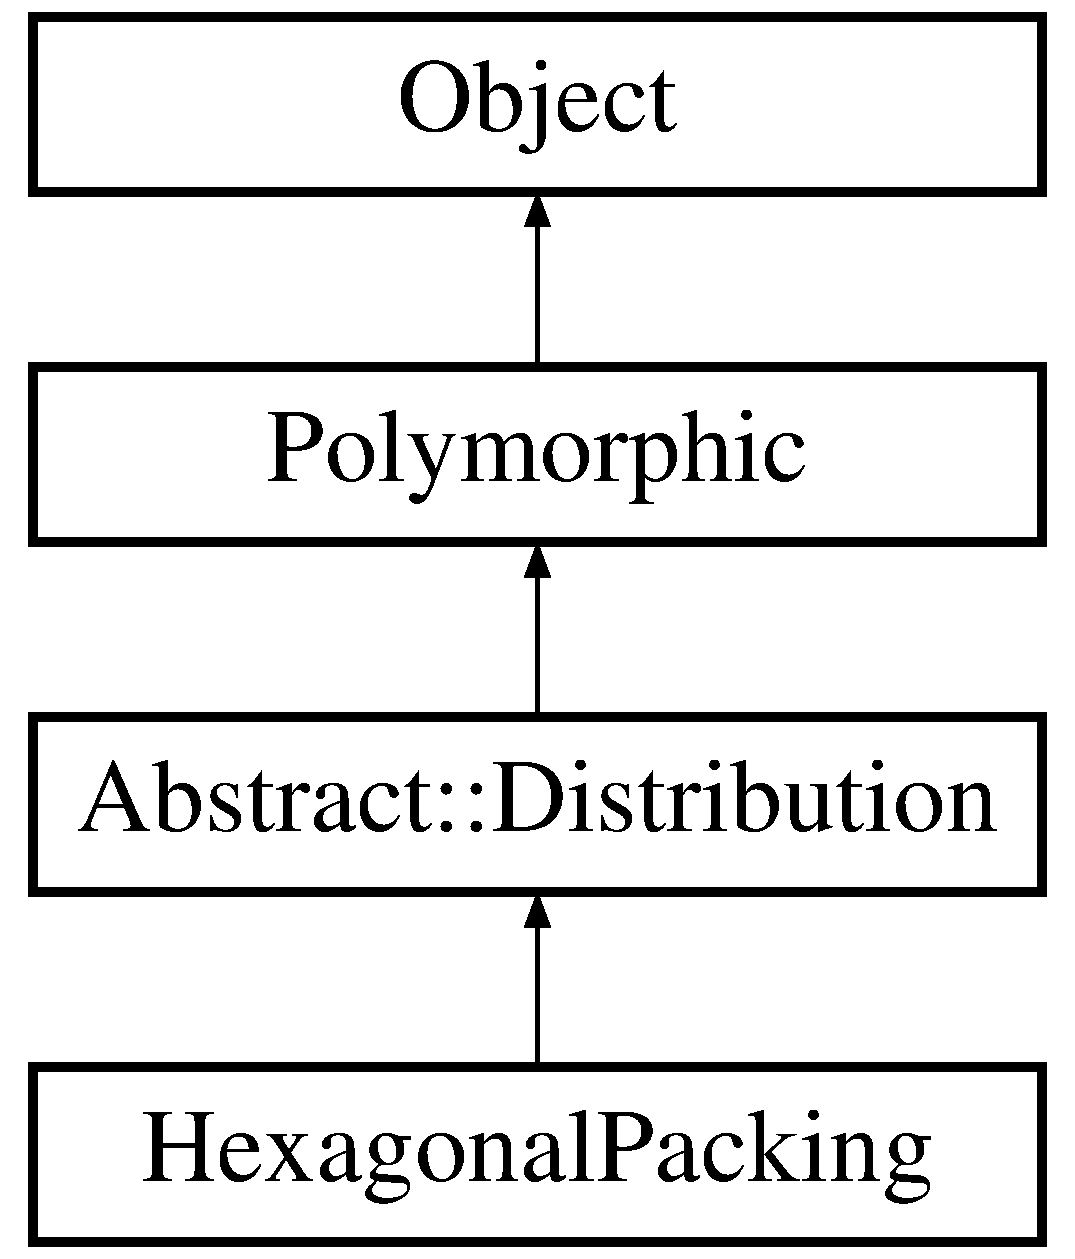
\includegraphics[height=4.000000cm]{classHexagonalPacking}
\end{center}
\end{figure}
\subsection*{Public Member Functions}
\begin{DoxyCompactItemize}
\item 
virtual \hyperlink{classArray}{Array}$<$ \hyperlink{classBasicVector}{Vector} $>$ \hyperlink{classHexagonalPacking_a276079137928da5c94f8bb870b038c4a}{generate} (const int n, const \hyperlink{classAbstract_1_1Domain}{Abstract\+::\+Domain} $\ast$domain) const override
\end{DoxyCompactItemize}


\subsection{Detailed Description}
Hexagonal close packing. 

\subsection{Member Function Documentation}
\hypertarget{classHexagonalPacking_a276079137928da5c94f8bb870b038c4a}{}\label{classHexagonalPacking_a276079137928da5c94f8bb870b038c4a} 
\index{Hexagonal\+Packing@{Hexagonal\+Packing}!generate@{generate}}
\index{generate@{generate}!Hexagonal\+Packing@{Hexagonal\+Packing}}
\subsubsection{\texorpdfstring{generate()}{generate()}}
{\footnotesize\ttfamily virtual \hyperlink{classArray}{Array}$<$\hyperlink{classBasicVector}{Vector}$>$ Hexagonal\+Packing\+::generate (\begin{DoxyParamCaption}\item[{const int}]{n,  }\item[{const \hyperlink{classAbstract_1_1Domain}{Abstract\+::\+Domain} $\ast$}]{domain }\end{DoxyParamCaption}) const\hspace{0.3cm}{\ttfamily [inline]}, {\ttfamily [override]}, {\ttfamily [virtual]}}

Base class for generating vertices with specific distribution. Also generates corresponding smoothing lengths and save them as fourth component of the vector. 
\begin{DoxyParams}{Parameters}
{\em n} & Expected number of generated vertices. \\
\hline
{\em domain} & Computational domain where the vertices are distributed \\
\hline
\end{DoxyParams}
\begin{DoxyReturn}{Returns}
Output array of vertices. The total number of vertices can slightly differ from n. 
\end{DoxyReturn}
\begin{DoxyNote}{Note}
This method is expected to be called once at the beginning of the run, so we can return allocated array without worrying about performance costs here. 
\end{DoxyNote}
\begin{DoxyRefDesc}{Todo}
\item[\hyperlink{todo__todo000014}{Todo}]generalize to 1 and 2 dim \end{DoxyRefDesc}


\begin{DoxyRefDesc}{Todo}
\item[\hyperlink{todo__todo000015}{Todo}]!!! \end{DoxyRefDesc}


Implements \hyperlink{classAbstract_1_1Distribution_aefb835b4c4d2d0a5f864bc2cee0492b2}{Abstract\+::\+Distribution}.



The documentation for this class was generated from the following file\+:\begin{DoxyCompactItemize}
\item 
/home/pavel/projects/astro/sph2/src/initconds/initconds.\+h\end{DoxyCompactItemize}

\hypertarget{classIdealGas}{}\section{Ideal\+Gas Class Reference}
\label{classIdealGas}\index{Ideal\+Gas@{Ideal\+Gas}}


Equation of state for ideal gas.  




{\ttfamily \#include $<$eos.\+h$>$}

Inheritance diagram for Ideal\+Gas\+:\begin{figure}[H]
\begin{center}
\leavevmode
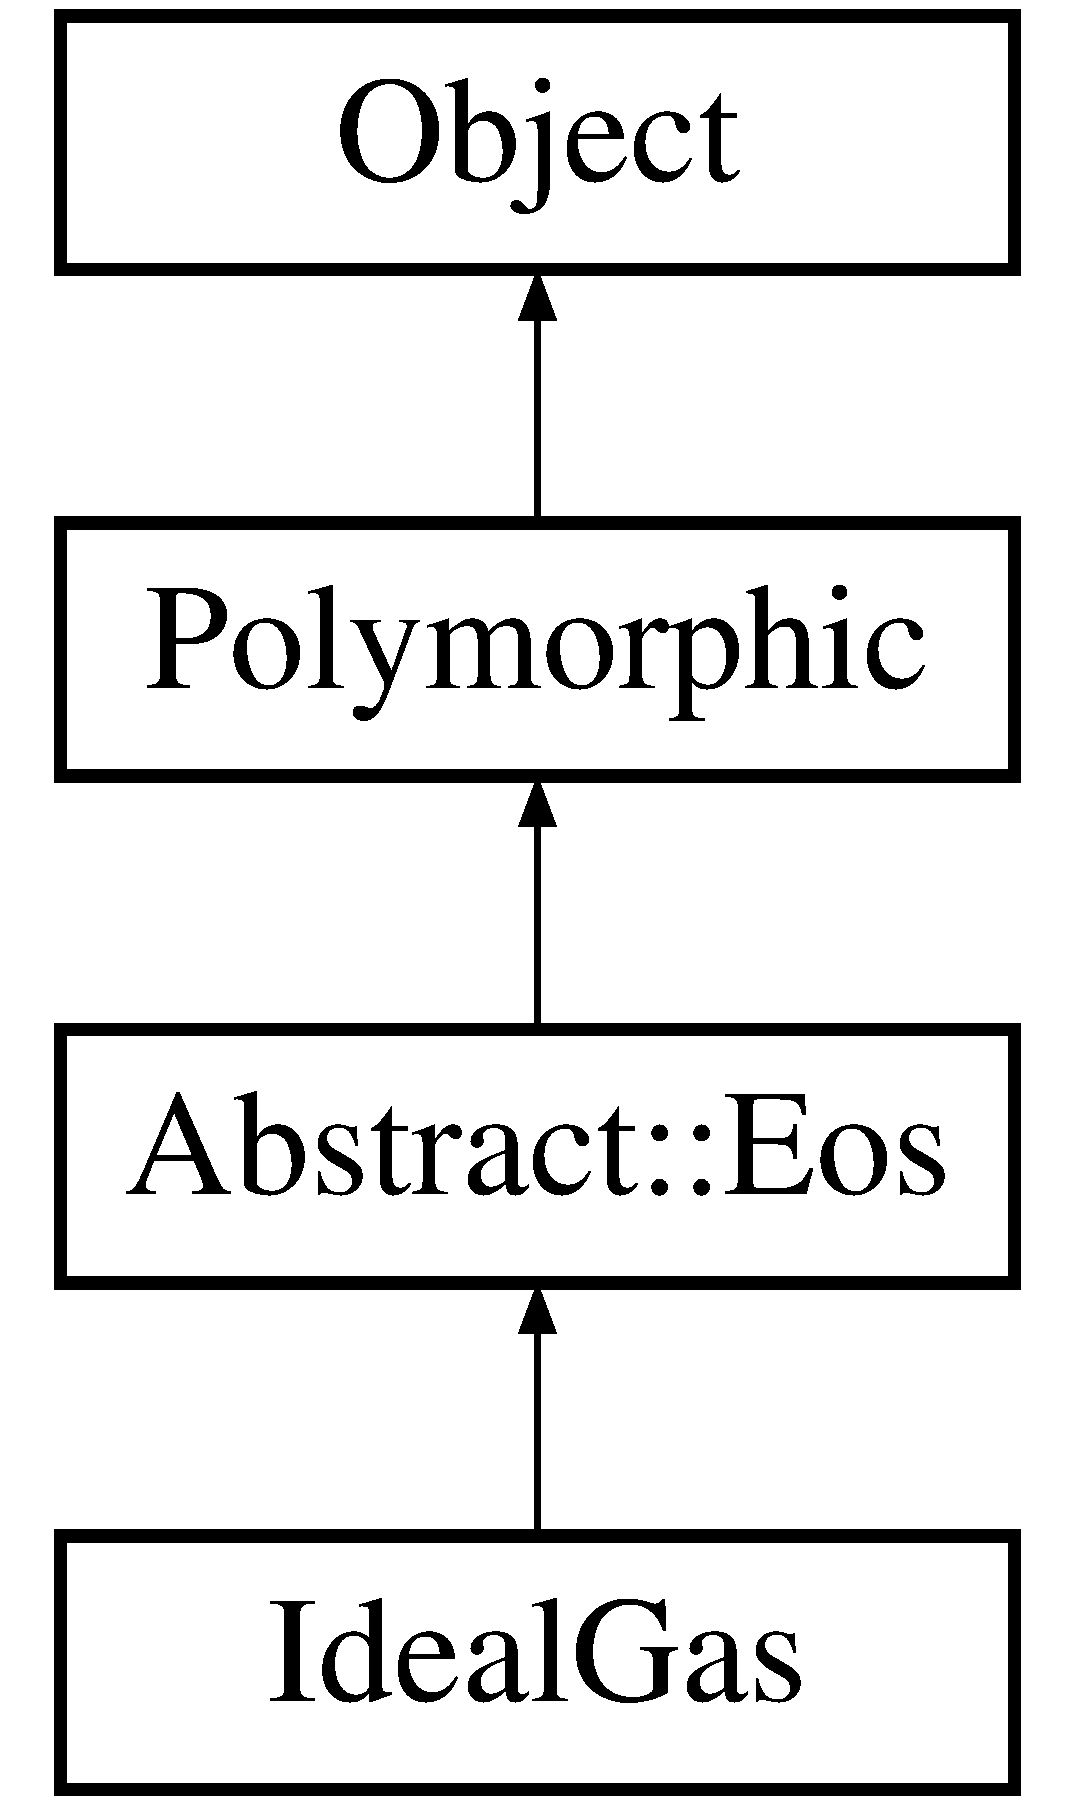
\includegraphics[height=4.000000cm]{classIdealGas}
\end{center}
\end{figure}
\subsection*{Public Member Functions}
\begin{DoxyCompactItemize}
\item 
\hypertarget{classIdealGas_af250b5658ce51009456179871042a230}{}\label{classIdealGas_af250b5658ce51009456179871042a230} 
{\bfseries Ideal\+Gas} (const Float gamma=1.\+5\+\_\+f)
\item 
virtual void \hyperlink{classIdealGas_a27ee0a167bbb7e5690ce6db5fca39ba1}{get\+Pressure} (\hyperlink{classArrayView}{Array\+View}$<$ const Float $>$ rho, \hyperlink{classArrayView}{Array\+View}$<$ const Float $>$ u, \hyperlink{classArrayView}{Array\+View}$<$ Float $>$ p) override
\item 
\hypertarget{classIdealGas_a58790f488c2e64054514de0ee170a268}{}\label{classIdealGas_a58790f488c2e64054514de0ee170a268} 
Float {\bfseries get\+Temperature} (const Float u)
\end{DoxyCompactItemize}


\subsection{Detailed Description}
Equation of state for ideal gas. 

\subsection{Member Function Documentation}
\hypertarget{classIdealGas_a27ee0a167bbb7e5690ce6db5fca39ba1}{}\label{classIdealGas_a27ee0a167bbb7e5690ce6db5fca39ba1} 
\index{Ideal\+Gas@{Ideal\+Gas}!get\+Pressure@{get\+Pressure}}
\index{get\+Pressure@{get\+Pressure}!Ideal\+Gas@{Ideal\+Gas}}
\subsubsection{\texorpdfstring{get\+Pressure()}{getPressure()}}
{\footnotesize\ttfamily virtual void Ideal\+Gas\+::get\+Pressure (\begin{DoxyParamCaption}\item[{\hyperlink{classArrayView}{Array\+View}$<$ const Float $>$}]{rho,  }\item[{\hyperlink{classArrayView}{Array\+View}$<$ const Float $>$}]{u,  }\item[{\hyperlink{classArrayView}{Array\+View}$<$ Float $>$}]{p }\end{DoxyParamCaption})\hspace{0.3cm}{\ttfamily [inline]}, {\ttfamily [override]}, {\ttfamily [virtual]}}

Computes a pressure from given density. \begin{DoxyRefDesc}{Todo}
\item[\hyperlink{todo__todo000018}{Todo}]EoS have more general relations, like P = P(rho, T) or P = P(rho, u) 

maybe pass model as a parameter? \end{DoxyRefDesc}


Implements \hyperlink{classAbstract_1_1Eos_ab21906f5fc78370a10cdbf97983544ea}{Abstract\+::\+Eos}.



The documentation for this class was generated from the following file\+:\begin{DoxyCompactItemize}
\item 
/home/pavel/projects/astro/sph2/src/physics/eos.\+h\end{DoxyCompactItemize}

\hypertarget{structIgnore}{}\section{Ignore Struct Reference}
\label{structIgnore}\index{Ignore@{Ignore}}


placeholder for unused variables in  




{\ttfamily \#include $<$tuple.\+h$>$}

\subsection*{Public Member Functions}
\begin{DoxyCompactItemize}
\item 
\hypertarget{structIgnore_a2c0d0d3c5a5ac93b1839103b1b0dafba}{}\label{structIgnore_a2c0d0d3c5a5ac93b1839103b1b0dafba} 
{\footnotesize template$<$class T $>$ }\\const \hyperlink{structIgnore}{Ignore} \& {\bfseries operator=} (const T \&) const
\end{DoxyCompactItemize}


\subsection{Detailed Description}
placeholder for unused variables in 

The documentation for this struct was generated from the following file\+:\begin{DoxyCompactItemize}
\item 
/home/pavel/projects/astro/sph2/src/structs/tuple.\+h\end{DoxyCompactItemize}

\hypertarget{structIndexCast}{}\section{Index\+Cast$<$ T1, T2 $>$ Struct Template Reference}
\label{structIndexCast}\index{Index\+Cast$<$ T1, T2 $>$@{Index\+Cast$<$ T1, T2 $>$}}
\subsection*{Static Public Member Functions}
\begin{DoxyCompactItemize}
\item 
\hypertarget{structIndexCast_a4649faea0aea9ac405862853b3a4c748}{}\label{structIndexCast_a4649faea0aea9ac405862853b3a4c748} 
{\footnotesize template$<$typename T $>$ }\\static T1 \& {\bfseries cast} (T \&\&value)
\end{DoxyCompactItemize}


The documentation for this struct was generated from the following file\+:\begin{DoxyCompactItemize}
\item 
/home/pavel/projects/astro/sph2/src/geometry/indices.\+h\end{DoxyCompactItemize}

\hypertarget{structIndexCast_3_01T1_00_01T1_01_4}{}\section{Index\+Cast$<$ T1, T1 $>$ Struct Template Reference}
\label{structIndexCast_3_01T1_00_01T1_01_4}\index{Index\+Cast$<$ T1, T1 $>$@{Index\+Cast$<$ T1, T1 $>$}}
\subsection*{Static Public Member Functions}
\begin{DoxyCompactItemize}
\item 
\hypertarget{structIndexCast_3_01T1_00_01T1_01_4_a7fe16b3c27e5aac6e4a65bd2cdff5380}{}\label{structIndexCast_3_01T1_00_01T1_01_4_a7fe16b3c27e5aac6e4a65bd2cdff5380} 
{\footnotesize template$<$typename T $>$ }\\static T \& {\bfseries cast} (T \&\&value)
\end{DoxyCompactItemize}


The documentation for this struct was generated from the following file\+:\begin{DoxyCompactItemize}
\item 
/home/pavel/projects/astro/sph2/src/geometry/indices.\+h\end{DoxyCompactItemize}

\hypertarget{structSph_1_1IndexDist__Sorter}{}\section{Sph\+:\+:Index\+Dist\+\_\+\+Sorter Struct Reference}
\label{structSph_1_1IndexDist__Sorter}\index{Sph\+::\+Index\+Dist\+\_\+\+Sorter@{Sph\+::\+Index\+Dist\+\_\+\+Sorter}}


{\ttfamily \#include $<$nanoflann.\+h$>$}

\subsection*{Public Member Functions}
\begin{DoxyCompactItemize}
\item 
{\footnotesize template$<$typename Pair\+Type $>$ }\\bool \hyperlink{structSph_1_1IndexDist__Sorter_a2f0133e7c5b4fa6c36975980ce8255c6}{operator()} (const Pair\+Type \&p1, const Pair\+Type \&p2) const
\end{DoxyCompactItemize}


\subsection{Detailed Description}
operator \char`\"{}$<$\char`\"{} for std\+::sort() 

\subsection{Member Function Documentation}
\hypertarget{structSph_1_1IndexDist__Sorter_a2f0133e7c5b4fa6c36975980ce8255c6}{}\label{structSph_1_1IndexDist__Sorter_a2f0133e7c5b4fa6c36975980ce8255c6} 
\index{Sph\+::\+Index\+Dist\+\_\+\+Sorter@{Sph\+::\+Index\+Dist\+\_\+\+Sorter}!operator()@{operator()}}
\index{operator()@{operator()}!Sph\+::\+Index\+Dist\+\_\+\+Sorter@{Sph\+::\+Index\+Dist\+\_\+\+Sorter}}
\subsubsection{\texorpdfstring{operator()()}{operator()()}}
{\footnotesize\ttfamily template$<$typename Pair\+Type $>$ \\
bool Sph\+::\+Index\+Dist\+\_\+\+Sorter\+::operator() (\begin{DoxyParamCaption}\item[{const Pair\+Type \&}]{p1,  }\item[{const Pair\+Type \&}]{p2 }\end{DoxyParamCaption}) const\hspace{0.3cm}{\ttfamily [inline]}}

Pair\+Type will be typically\+: std\+::pair$<$\+Index\+Type,\+Distance\+Type$>$ 

The documentation for this struct was generated from the following file\+:\begin{DoxyCompactItemize}
\item 
/home/pavel/projects/astro/sph2/src/tree/nanoflann.\+h\end{DoxyCompactItemize}

\hypertarget{classIntegrator}{}\section{Integrator$<$ T\+Rng, T\+Internal $>$ Class Template Reference}
\label{classIntegrator}\index{Integrator$<$ T\+Rng, T\+Internal $>$@{Integrator$<$ T\+Rng, T\+Internal $>$}}


\hyperlink{classObject}{Object} for integrating a generic scalar function.  




{\ttfamily \#include $<$integrator.\+h$>$}

Inheritance diagram for Integrator$<$ T\+Rng, T\+Internal $>$\+:\begin{figure}[H]
\begin{center}
\leavevmode
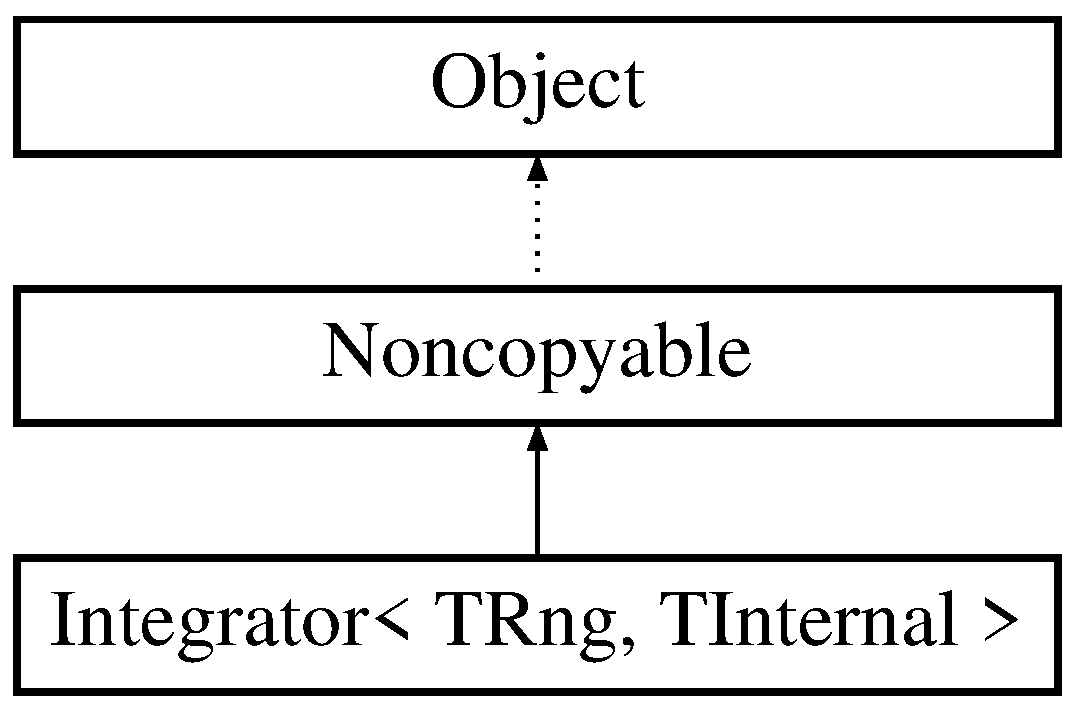
\includegraphics[height=3.000000cm]{classIntegrator}
\end{center}
\end{figure}
\subsection*{Public Member Functions}
\begin{DoxyCompactItemize}
\item 
\hypertarget{classIntegrator_a8f83bdb5012e5cea5b2cc566c2b4f207}{}\label{classIntegrator_a8f83bdb5012e5cea5b2cc566c2b4f207} 
\hyperlink{classIntegrator_a8f83bdb5012e5cea5b2cc566c2b4f207}{Integrator} (\hyperlink{classAbstract_1_1Domain}{Abstract\+::\+Domain} $\ast$domain)
\begin{DoxyCompactList}\small\item\em Constructs an integrator given domain of integration. \end{DoxyCompactList}\item 
{\footnotesize template$<$typename T\+Functor $>$ }\\auto \hyperlink{classIntegrator_adf117e3936f928bccd93ad41567acba8}{integrate} (T\+Functor \&\&f, const Float target\+Error=0.\+001\+\_\+f)
\end{DoxyCompactItemize}


\subsection{Detailed Description}
\subsubsection*{template$<$typename T\+Rng = Uniform\+Rng, typename T\+Internal = double$>$\newline
class Integrator$<$ T\+Rng, T\+Internal $>$}

\hyperlink{classObject}{Object} for integrating a generic scalar function. 

\subsection{Member Function Documentation}
\hypertarget{classIntegrator_adf117e3936f928bccd93ad41567acba8}{}\label{classIntegrator_adf117e3936f928bccd93ad41567acba8} 
\index{Integrator@{Integrator}!integrate@{integrate}}
\index{integrate@{integrate}!Integrator@{Integrator}}
\subsubsection{\texorpdfstring{integrate()}{integrate()}}
{\footnotesize\ttfamily template$<$typename T\+Rng  = Uniform\+Rng, typename T\+Internal  = double$>$ \\
template$<$typename T\+Functor $>$ \\
auto \hyperlink{classIntegrator}{Integrator}$<$ T\+Rng, T\+Internal $>$\+::integrate (\begin{DoxyParamCaption}\item[{T\+Functor \&\&}]{f,  }\item[{const Float}]{target\+Error = {\ttfamily 0.001\+\_\+f} }\end{DoxyParamCaption})\hspace{0.3cm}{\ttfamily [inline]}}

Integrate a function. 
\begin{DoxyParams}{Parameters}
{\em f} & Functor with a parameter Vector$<$\+T, d$>$, returning a scalar value (of type T) \\
\hline
{\em target\+Error} & Precision of the integral. Note that half error means approximately four times the computation time. \\
\hline
\end{DoxyParams}
\begin{DoxyRefDesc}{Todo}
\item[\hyperlink{todo__todo000003}{Todo}]number of components must be d !! \end{DoxyRefDesc}


The documentation for this class was generated from the following file\+:\begin{DoxyCompactItemize}
\item 
/home/pavel/projects/astro/sph2/src/core/integrator.\+h\end{DoxyCompactItemize}

\hypertarget{structSph_1_1KDTreeSingleIndexAdaptor_1_1Interval}{}\section{Sph\+:\+:K\+D\+Tree\+Single\+Index\+Adaptor$<$ Distance, Dataset\+Adaptor, D\+IM, Index\+Type $>$\+:\+:Interval Struct Reference}
\label{structSph_1_1KDTreeSingleIndexAdaptor_1_1Interval}\index{Sph\+::\+K\+D\+Tree\+Single\+Index\+Adaptor$<$ Distance, Dataset\+Adaptor, D\+I\+M, Index\+Type $>$\+::\+Interval@{Sph\+::\+K\+D\+Tree\+Single\+Index\+Adaptor$<$ Distance, Dataset\+Adaptor, D\+I\+M, Index\+Type $>$\+::\+Interval}}
\subsection*{Public Attributes}
\begin{DoxyCompactItemize}
\item 
\hypertarget{structSph_1_1KDTreeSingleIndexAdaptor_1_1Interval_a3ead59019eab5a1268327047a6137ffc}{}\label{structSph_1_1KDTreeSingleIndexAdaptor_1_1Interval_a3ead59019eab5a1268327047a6137ffc} 
Element\+Type {\bfseries low}
\item 
\hypertarget{structSph_1_1KDTreeSingleIndexAdaptor_1_1Interval_aba3f07308ce8ad9b082c6d789f84f996}{}\label{structSph_1_1KDTreeSingleIndexAdaptor_1_1Interval_aba3f07308ce8ad9b082c6d789f84f996} 
Element\+Type {\bfseries high}
\end{DoxyCompactItemize}


The documentation for this struct was generated from the following file\+:\begin{DoxyCompactItemize}
\item 
/home/pavel/projects/astro/sph2/src/tree/nanoflann.\+h\end{DoxyCompactItemize}

\hypertarget{structIsAngularType}{}\section{Is\+Angular\+Type$<$ T $>$ Struct Template Reference}
\label{structIsAngularType}\index{Is\+Angular\+Type$<$ T $>$@{Is\+Angular\+Type$<$ T $>$}}


Is angular unit (degrees or radians)?  




{\ttfamily \#include $<$traits.\+h$>$}

\subsection*{Static Public Attributes}
\begin{DoxyCompactItemize}
\item 
\hypertarget{structIsAngularType_ace623476ee3483065c0b71a4853cca2e}{}\label{structIsAngularType_ace623476ee3483065c0b71a4853cca2e} 
static constexpr bool {\bfseries value} = true
\end{DoxyCompactItemize}


\subsection{Detailed Description}
\subsubsection*{template$<$typename T$>$\newline
struct Is\+Angular\+Type$<$ T $>$}

Is angular unit (degrees or radians)? 

The documentation for this struct was generated from the following file\+:\begin{DoxyCompactItemize}
\item 
/home/pavel/projects/astro/sph2/src/core/traits.\+h\end{DoxyCompactItemize}

\hypertarget{structIsBaseAllType}{}\section{Is\+Base\+All\+Type$<$ T\+Base, T\+Args $>$ Struct Template Reference}
\label{structIsBaseAllType}\index{Is\+Base\+All\+Type$<$ T\+Base, T\+Args $>$@{Is\+Base\+All\+Type$<$ T\+Base, T\+Args $>$}}


A test if all types have the same common base T\+Base.  




{\ttfamily \#include $<$traits.\+h$>$}



\subsection{Detailed Description}
\subsubsection*{template$<$typename T\+Base, typename... T\+Args$>$\newline
struct Is\+Base\+All\+Type$<$ T\+Base, T\+Args $>$}

A test if all types have the same common base T\+Base. 

The documentation for this struct was generated from the following file\+:\begin{DoxyCompactItemize}
\item 
/home/pavel/projects/astro/sph2/src/core/traits.\+h\end{DoxyCompactItemize}

\hypertarget{structIsBaseAllType_3_01TBase_00_01T0_01_4}{}\section{Is\+Base\+All\+Type$<$ T\+Base, T0 $>$ Struct Template Reference}
\label{structIsBaseAllType_3_01TBase_00_01T0_01_4}\index{Is\+Base\+All\+Type$<$ T\+Base, T0 $>$@{Is\+Base\+All\+Type$<$ T\+Base, T0 $>$}}
\subsection*{Static Public Attributes}
\begin{DoxyCompactItemize}
\item 
\hypertarget{structIsBaseAllType_3_01TBase_00_01T0_01_4_a4059500c5a67420cb879703f0cd8e712}{}\label{structIsBaseAllType_3_01TBase_00_01T0_01_4_a4059500c5a67420cb879703f0cd8e712} 
static constexpr bool {\bfseries value} = Is\+Base$<$T0, T\+Base$>$
\end{DoxyCompactItemize}


The documentation for this struct was generated from the following file\+:\begin{DoxyCompactItemize}
\item 
/home/pavel/projects/astro/sph2/src/core/traits.\+h\end{DoxyCompactItemize}

\hypertarget{structIsBaseAllType_3_01TBase_00_01T0_00_01TArgs_8_8_8_01_4}{}\section{Is\+Base\+All\+Type$<$ T\+Base, T0, T\+Args... $>$ Struct Template Reference}
\label{structIsBaseAllType_3_01TBase_00_01T0_00_01TArgs_8_8_8_01_4}\index{Is\+Base\+All\+Type$<$ T\+Base, T0, T\+Args... $>$@{Is\+Base\+All\+Type$<$ T\+Base, T0, T\+Args... $>$}}
\subsection*{Static Public Attributes}
\begin{DoxyCompactItemize}
\item 
\hypertarget{structIsBaseAllType_3_01TBase_00_01T0_00_01TArgs_8_8_8_01_4_acf2b6f6acfecbbb4327fe2e22a132935}{}\label{structIsBaseAllType_3_01TBase_00_01T0_00_01TArgs_8_8_8_01_4_acf2b6f6acfecbbb4327fe2e22a132935} 
static constexpr bool {\bfseries value} = \hyperlink{structIsBaseAllType}{Is\+Base\+All\+Type}$<$T\+Base, T\+Args...$>$\+::value \&\& Is\+Base$<$T0, T\+Base$>$
\end{DoxyCompactItemize}


The documentation for this struct was generated from the following file\+:\begin{DoxyCompactItemize}
\item 
/home/pavel/projects/astro/sph2/src/core/traits.\+h\end{DoxyCompactItemize}

\hypertarget{structIsBaseType}{}\section{Is\+Base\+Type$<$ T, T\+Base, typename $>$ Struct Template Reference}
\label{structIsBaseType}\index{Is\+Base\+Type$<$ T, T\+Base, typename $>$@{Is\+Base\+Type$<$ T, T\+Base, typename $>$}}


A test if the the type T has a base T\+Base.  




{\ttfamily \#include $<$traits.\+h$>$}

\subsection*{Static Public Attributes}
\begin{DoxyCompactItemize}
\item 
\hypertarget{structIsBaseType_aafb26a2b86a7f915f874fd64476e026a}{}\label{structIsBaseType_aafb26a2b86a7f915f874fd64476e026a} 
static constexpr bool {\bfseries value} = false
\end{DoxyCompactItemize}


\subsection{Detailed Description}
\subsubsection*{template$<$typename T, typename T\+Base, typename = void$>$\newline
struct Is\+Base\+Type$<$ T, T\+Base, typename $>$}

A test if the the type T has a base T\+Base. 

The documentation for this struct was generated from the following file\+:\begin{DoxyCompactItemize}
\item 
/home/pavel/projects/astro/sph2/src/core/traits.\+h\end{DoxyCompactItemize}

\hypertarget{structIsBaseType_3_01T_00_01TBase_00_01std_1_1enable__if__t_3_01std_1_1is__same_3_01Base_3_01T_0c0a7ea670c56e23cbe6d6f78f2838e45}{}\section{Is\+Base\+Type$<$ T, T\+Base, std\+:\+:enable\+\_\+if\+\_\+t$<$ std\+:\+:is\+\_\+same$<$ Base$<$ T $>$, T\+Base $>$\+:\+:value $>$ $>$ Struct Template Reference}
\label{structIsBaseType_3_01T_00_01TBase_00_01std_1_1enable__if__t_3_01std_1_1is__same_3_01Base_3_01T_0c0a7ea670c56e23cbe6d6f78f2838e45}\index{Is\+Base\+Type$<$ T, T\+Base, std\+::enable\+\_\+if\+\_\+t$<$ std\+::is\+\_\+same$<$ Base$<$ T $>$, T\+Base $>$\+::value $>$ $>$@{Is\+Base\+Type$<$ T, T\+Base, std\+::enable\+\_\+if\+\_\+t$<$ std\+::is\+\_\+same$<$ Base$<$ T $>$, T\+Base $>$\+::value $>$ $>$}}
\subsection*{Static Public Attributes}
\begin{DoxyCompactItemize}
\item 
\hypertarget{structIsBaseType_3_01T_00_01TBase_00_01std_1_1enable__if__t_3_01std_1_1is__same_3_01Base_3_01T_0c0a7ea670c56e23cbe6d6f78f2838e45_a36f202b553ef5cc569102f67623a2857}{}\label{structIsBaseType_3_01T_00_01TBase_00_01std_1_1enable__if__t_3_01std_1_1is__same_3_01Base_3_01T_0c0a7ea670c56e23cbe6d6f78f2838e45_a36f202b553ef5cc569102f67623a2857} 
static constexpr bool {\bfseries value} = true
\end{DoxyCompactItemize}


The documentation for this struct was generated from the following file\+:\begin{DoxyCompactItemize}
\item 
/home/pavel/projects/astro/sph2/src/core/traits.\+h\end{DoxyCompactItemize}

\hypertarget{structIsDimensionlessType}{}\section{Is\+Dimensionless\+Type$<$ T $>$ Struct Template Reference}
\label{structIsDimensionlessType}\index{Is\+Dimensionless\+Type$<$ T $>$@{Is\+Dimensionless\+Type$<$ T $>$}}


Is dimensionless?  




{\ttfamily \#include $<$traits.\+h$>$}

\subsection*{Static Public Attributes}
\begin{DoxyCompactItemize}
\item 
\hypertarget{structIsDimensionlessType_acf7d71c6c1406613b76e9622bbdb3016}{}\label{structIsDimensionlessType_acf7d71c6c1406613b76e9622bbdb3016} 
static constexpr bool {\bfseries value} = true
\end{DoxyCompactItemize}


\subsection{Detailed Description}
\subsubsection*{template$<$typename T$>$\newline
struct Is\+Dimensionless\+Type$<$ T $>$}

Is dimensionless? 

The documentation for this struct was generated from the following file\+:\begin{DoxyCompactItemize}
\item 
/home/pavel/projects/astro/sph2/src/core/traits.\+h\end{DoxyCompactItemize}

\hypertarget{structIsPowerType}{}\section{Is\+Power\+Type$<$ T, n $>$ Struct Template Reference}
\label{structIsPowerType}\index{Is\+Power\+Type$<$ T, n $>$@{Is\+Power\+Type$<$ T, n $>$}}


Is the type a n-\/th power?  




{\ttfamily \#include $<$traits.\+h$>$}

\subsection*{Static Public Attributes}
\begin{DoxyCompactItemize}
\item 
\hypertarget{structIsPowerType_ada1ae20e8cee5ef6f30d63944e9f8300}{}\label{structIsPowerType_ada1ae20e8cee5ef6f30d63944e9f8300} 
static constexpr bool {\bfseries value} = true
\end{DoxyCompactItemize}


\subsection{Detailed Description}
\subsubsection*{template$<$typename T, int n$>$\newline
struct Is\+Power\+Type$<$ T, n $>$}

Is the type a n-\/th power? 

The documentation for this struct was generated from the following file\+:\begin{DoxyCompactItemize}
\item 
/home/pavel/projects/astro/sph2/src/core/traits.\+h\end{DoxyCompactItemize}

\hypertarget{structIsValueOfPrecisionType}{}\section{Is\+Value\+Of\+Precision\+Type$<$ T, T\+Precision $>$ Struct Template Reference}
\label{structIsValueOfPrecisionType}\index{Is\+Value\+Of\+Precision\+Type$<$ T, T\+Precision $>$@{Is\+Value\+Of\+Precision\+Type$<$ T, T\+Precision $>$}}


{\ttfamily \#include $<$traits.\+h$>$}

\subsection*{Static Public Attributes}
\begin{DoxyCompactItemize}
\item 
\hypertarget{structIsValueOfPrecisionType_a41933c85d20b23070f255ffd03f0e0a4}{}\label{structIsValueOfPrecisionType_a41933c85d20b23070f255ffd03f0e0a4} 
static constexpr bool {\bfseries value} = false
\end{DoxyCompactItemize}


\subsection{Detailed Description}
\subsubsection*{template$<$typename T, typename T\+Precision$>$\newline
struct Is\+Value\+Of\+Precision\+Type$<$ T, T\+Precision $>$}

Trait to check if the type is a value (see \hyperlink{structIsValueType}{Is\+Value\+Type}) A\+ND if the base type of the value has given precision. 

The documentation for this struct was generated from the following file\+:\begin{DoxyCompactItemize}
\item 
/home/pavel/projects/astro/sph2/src/core/traits.\+h\end{DoxyCompactItemize}

\hypertarget{structIsValueOfPrecisionType_3_01double_00_01double_01_4}{}\section{Is\+Value\+Of\+Precision\+Type$<$ double, double $>$ Struct Template Reference}
\label{structIsValueOfPrecisionType_3_01double_00_01double_01_4}\index{Is\+Value\+Of\+Precision\+Type$<$ double, double $>$@{Is\+Value\+Of\+Precision\+Type$<$ double, double $>$}}
\subsection*{Static Public Attributes}
\begin{DoxyCompactItemize}
\item 
\hypertarget{structIsValueOfPrecisionType_3_01double_00_01double_01_4_aa9a9861d72d5cb0aa1f62012f71c2b1e}{}\label{structIsValueOfPrecisionType_3_01double_00_01double_01_4_aa9a9861d72d5cb0aa1f62012f71c2b1e} 
static constexpr bool {\bfseries value} = true
\end{DoxyCompactItemize}


The documentation for this struct was generated from the following file\+:\begin{DoxyCompactItemize}
\item 
/home/pavel/projects/astro/sph2/src/core/traits.\+h\end{DoxyCompactItemize}

\hypertarget{structIsValueOfPrecisionType_3_01float_00_01float_01_4}{}\section{Is\+Value\+Of\+Precision\+Type$<$ float, float $>$ Struct Template Reference}
\label{structIsValueOfPrecisionType_3_01float_00_01float_01_4}\index{Is\+Value\+Of\+Precision\+Type$<$ float, float $>$@{Is\+Value\+Of\+Precision\+Type$<$ float, float $>$}}
\subsection*{Static Public Attributes}
\begin{DoxyCompactItemize}
\item 
\hypertarget{structIsValueOfPrecisionType_3_01float_00_01float_01_4_a457225d78afeb7ab06359e698b7d4cef}{}\label{structIsValueOfPrecisionType_3_01float_00_01float_01_4_a457225d78afeb7ab06359e698b7d4cef} 
static constexpr bool {\bfseries value} = true
\end{DoxyCompactItemize}


The documentation for this struct was generated from the following file\+:\begin{DoxyCompactItemize}
\item 
/home/pavel/projects/astro/sph2/src/core/traits.\+h\end{DoxyCompactItemize}

\hypertarget{structIsValueType}{}\section{Is\+Value\+Type$<$ T $>$ Struct Template Reference}
\label{structIsValueType}\index{Is\+Value\+Type$<$ T $>$@{Is\+Value\+Type$<$ T $>$}}


{\ttfamily \#include $<$traits.\+h$>$}

\subsection*{Static Public Attributes}
\begin{DoxyCompactItemize}
\item 
\hypertarget{structIsValueType_ab5f586eb43a336b367e924fda58a935a}{}\label{structIsValueType_ab5f586eb43a336b367e924fda58a935a} 
static constexpr bool {\bfseries value} = false
\end{DoxyCompactItemize}


\subsection{Detailed Description}
\subsubsection*{template$<$typename T$>$\newline
struct Is\+Value\+Type$<$ T $>$}

Trait to determine whether the type is a struct holding a single value with (at least explicit) conversion and cast operators defined. False by default, need to be specialized if one wishes to use certain struct (like units) instead of ordinary floating-\/point variables in algorithms. 

The documentation for this struct was generated from the following file\+:\begin{DoxyCompactItemize}
\item 
/home/pavel/projects/astro/sph2/src/core/traits.\+h\end{DoxyCompactItemize}

\hypertarget{structIsValueType_3_01double_01_4}{}\section{Is\+Value\+Type$<$ double $>$ Struct Template Reference}
\label{structIsValueType_3_01double_01_4}\index{Is\+Value\+Type$<$ double $>$@{Is\+Value\+Type$<$ double $>$}}
\subsection*{Static Public Attributes}
\begin{DoxyCompactItemize}
\item 
\hypertarget{structIsValueType_3_01double_01_4_a549187b8340852dfd8538023625f5ee2}{}\label{structIsValueType_3_01double_01_4_a549187b8340852dfd8538023625f5ee2} 
static constexpr bool {\bfseries value} = true
\end{DoxyCompactItemize}


The documentation for this struct was generated from the following file\+:\begin{DoxyCompactItemize}
\item 
/home/pavel/projects/astro/sph2/src/core/traits.\+h\end{DoxyCompactItemize}

\hypertarget{structIsValueType_3_01float_01_4}{}\section{Is\+Value\+Type$<$ float $>$ Struct Template Reference}
\label{structIsValueType_3_01float_01_4}\index{Is\+Value\+Type$<$ float $>$@{Is\+Value\+Type$<$ float $>$}}
\subsection*{Static Public Attributes}
\begin{DoxyCompactItemize}
\item 
\hypertarget{structIsValueType_3_01float_01_4_a8813074466c5bfacc128beef976fa45a}{}\label{structIsValueType_3_01float_01_4_a8813074466c5bfacc128beef976fa45a} 
static constexpr bool {\bfseries value} = true
\end{DoxyCompactItemize}


The documentation for this struct was generated from the following file\+:\begin{DoxyCompactItemize}
\item 
/home/pavel/projects/astro/sph2/src/core/traits.\+h\end{DoxyCompactItemize}

\hypertarget{structIsVectorType}{}\section{Is\+Vector\+Type$<$ T $>$ Struct Template Reference}
\label{structIsVectorType}\index{Is\+Vector\+Type$<$ T $>$@{Is\+Vector\+Type$<$ T $>$}}


Helper type trait to determine if the type is a vector of some kind.  




{\ttfamily \#include $<$vector.\+h$>$}

\subsection*{Static Public Attributes}
\begin{DoxyCompactItemize}
\item 
\hypertarget{structIsVectorType_afdf963da742e2c4b725e0e1f6390feda}{}\label{structIsVectorType_afdf963da742e2c4b725e0e1f6390feda} 
static constexpr bool {\bfseries value} = false
\end{DoxyCompactItemize}


\subsection{Detailed Description}
\subsubsection*{template$<$typename T$>$\newline
struct Is\+Vector\+Type$<$ T $>$}

Helper type trait to determine if the type is a vector of some kind. 

The documentation for this struct was generated from the following file\+:\begin{DoxyCompactItemize}
\item 
/home/pavel/projects/astro/sph2/src/geometry/vector.\+h\end{DoxyCompactItemize}

\hypertarget{structIsVectorType_3_01BasicVector_3_01T_01_4_01_4}{}\section{Is\+Vector\+Type$<$ Basic\+Vector$<$ T $>$ $>$ Struct Template Reference}
\label{structIsVectorType_3_01BasicVector_3_01T_01_4_01_4}\index{Is\+Vector\+Type$<$ Basic\+Vector$<$ T $>$ $>$@{Is\+Vector\+Type$<$ Basic\+Vector$<$ T $>$ $>$}}
\subsection*{Static Public Attributes}
\begin{DoxyCompactItemize}
\item 
\hypertarget{structIsVectorType_3_01BasicVector_3_01T_01_4_01_4_a7df80070d8e80465803010c069ed51e3}{}\label{structIsVectorType_3_01BasicVector_3_01T_01_4_01_4_a7df80070d8e80465803010c069ed51e3} 
static constexpr bool {\bfseries value} = true
\end{DoxyCompactItemize}


The documentation for this struct was generated from the following file\+:\begin{DoxyCompactItemize}
\item 
/home/pavel/projects/astro/sph2/src/geometry/vector.\+h\end{DoxyCompactItemize}

\hypertarget{classIterator}{}\section{Iterator$<$ T, T\+Counter $>$ Class Template Reference}
\label{classIterator}\index{Iterator$<$ T, T\+Counter $>$@{Iterator$<$ T, T\+Counter $>$}}
Inheritance diagram for Iterator$<$ T, T\+Counter $>$\+:\begin{figure}[H]
\begin{center}
\leavevmode
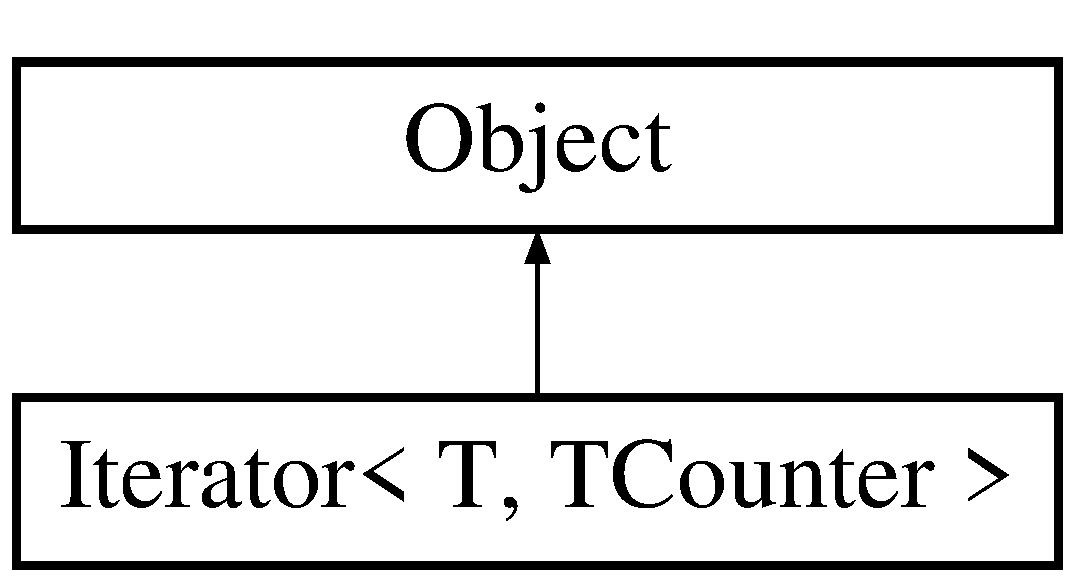
\includegraphics[height=2.000000cm]{classIterator}
\end{center}
\end{figure}
\subsection*{Public Types}
\begin{DoxyCompactItemize}
\item 
\hypertarget{classIterator_adef9395a4e35c735309294edc6dad06c}{}\label{classIterator_adef9395a4e35c735309294edc6dad06c} 
using {\bfseries iterator\+\_\+category} = std\+::random\+\_\+access\+\_\+iterator\+\_\+tag
\item 
\hypertarget{classIterator_a28722a581d52ff575f1d43119a9e9b76}{}\label{classIterator_a28722a581d52ff575f1d43119a9e9b76} 
using {\bfseries value\+\_\+type} = T
\item 
\hypertarget{classIterator_a4c323bdde2a1bb4e30f7cb16bfd9fc75}{}\label{classIterator_a4c323bdde2a1bb4e30f7cb16bfd9fc75} 
using {\bfseries difference\+\_\+type} = size\+\_\+t
\item 
\hypertarget{classIterator_aa550510e9ce3c7eb4bcf82f3a87f6e00}{}\label{classIterator_aa550510e9ce3c7eb4bcf82f3a87f6e00} 
using {\bfseries pointer} = T $\ast$
\item 
\hypertarget{classIterator_a6728a45fa20acfeedfde569360e2e5b3}{}\label{classIterator_a6728a45fa20acfeedfde569360e2e5b3} 
using {\bfseries reference} = T \&
\end{DoxyCompactItemize}
\subsection*{Public Member Functions}
\begin{DoxyCompactItemize}
\item 
\hypertarget{classIterator_a37682d15d8f14b6cce4a7950c7292867}{}\label{classIterator_a37682d15d8f14b6cce4a7950c7292867} 
const T \& {\bfseries operator$\ast$} () const
\item 
\hypertarget{classIterator_ae25de29205f6cdeefcd32fde37e4d5ca}{}\label{classIterator_ae25de29205f6cdeefcd32fde37e4d5ca} 
T \& {\bfseries operator$\ast$} ()
\item 
\hypertarget{classIterator_a681ddc4b43edb0fd4ca3c49884b77f07}{}\label{classIterator_a681ddc4b43edb0fd4ca3c49884b77f07} 
\hyperlink{classIterator}{Iterator} {\bfseries operator+} (const T\+Counter n) const
\item 
\hypertarget{classIterator_a489b8f3d0a34694a4c6776b6d420b029}{}\label{classIterator_a489b8f3d0a34694a4c6776b6d420b029} 
\hyperlink{classIterator}{Iterator} {\bfseries operator-\/} (const T\+Counter n) const
\item 
\hypertarget{classIterator_a3fa3e09e4060b0e1964aba189529ceac}{}\label{classIterator_a3fa3e09e4060b0e1964aba189529ceac} 
void {\bfseries operator+=} (const T\+Counter n)
\item 
\hypertarget{classIterator_a215fb6135627b9bca788de9192558375}{}\label{classIterator_a215fb6135627b9bca788de9192558375} 
void {\bfseries operator-\/=} (const T\+Counter n)
\item 
\hypertarget{classIterator_a9729d28b9acf45a8998cf0015946402b}{}\label{classIterator_a9729d28b9acf45a8998cf0015946402b} 
\hyperlink{classIterator}{Iterator} \& {\bfseries operator++} ()
\item 
\hypertarget{classIterator_a6d84895dd35fc52c9fbdaea622ed946e}{}\label{classIterator_a6d84895dd35fc52c9fbdaea622ed946e} 
\hyperlink{classIterator}{Iterator} {\bfseries operator++} (int)
\item 
\hypertarget{classIterator_a9e94f8acac03557f80a4c915baeba8fb}{}\label{classIterator_a9e94f8acac03557f80a4c915baeba8fb} 
\hyperlink{classIterator}{Iterator} \& {\bfseries operator-\/-\/} ()
\item 
\hypertarget{classIterator_a7bfadc053058436600ff02029a4287be}{}\label{classIterator_a7bfadc053058436600ff02029a4287be} 
\hyperlink{classIterator}{Iterator} {\bfseries operator-\/-\/} (int)
\item 
\hypertarget{classIterator_a7e9d9cb29073bcb84a2ea5535123b657}{}\label{classIterator_a7e9d9cb29073bcb84a2ea5535123b657} 
size\+\_\+t {\bfseries operator-\/} (const \hyperlink{classIterator}{Iterator} \&iter) const
\item 
\hypertarget{classIterator_a6d99a1e700d42466e0c14c91e87699b9}{}\label{classIterator_a6d99a1e700d42466e0c14c91e87699b9} 
bool {\bfseries operator$<$} (const \hyperlink{classIterator}{Iterator} \&iter) const
\item 
\hypertarget{classIterator_ae095b424d8866d2d60eaef1760fcacbe}{}\label{classIterator_ae095b424d8866d2d60eaef1760fcacbe} 
bool {\bfseries operator$>$} (const \hyperlink{classIterator}{Iterator} \&iter) const
\item 
\hypertarget{classIterator_a5d066a1f9dbbf95233d7bd44eb3484ae}{}\label{classIterator_a5d066a1f9dbbf95233d7bd44eb3484ae} 
bool {\bfseries operator$<$=} (const \hyperlink{classIterator}{Iterator} \&iter) const
\item 
\hypertarget{classIterator_ab50333dc2ff4fd6b1b23b7eb39b602ce}{}\label{classIterator_ab50333dc2ff4fd6b1b23b7eb39b602ce} 
bool {\bfseries operator$>$=} (const \hyperlink{classIterator}{Iterator} \&iter) const
\item 
\hypertarget{classIterator_aedd5367f618d50c0664c1e9e1caf848b}{}\label{classIterator_aedd5367f618d50c0664c1e9e1caf848b} 
bool {\bfseries operator==} (const \hyperlink{classIterator}{Iterator} \&iter) const
\item 
\hypertarget{classIterator_a2b19ea3c082f76a4497c5c8416fded92}{}\label{classIterator_a2b19ea3c082f76a4497c5c8416fded92} 
bool {\bfseries operator!=} (const \hyperlink{classIterator}{Iterator} \&iter) const
\end{DoxyCompactItemize}
\subsection*{Protected Member Functions}
\begin{DoxyCompactItemize}
\item 
\hypertarget{classIterator_ad38bf9cf53766a2adaf5a6654e3f3ac2}{}\label{classIterator_ad38bf9cf53766a2adaf5a6654e3f3ac2} 
{\bfseries Iterator} (T $\ast$data, const T $\ast$begin, const T $\ast$end)
\end{DoxyCompactItemize}
\subsection*{Protected Attributes}
\begin{DoxyCompactItemize}
\item 
\hypertarget{classIterator_a816091a33e21f9884091f7053f3dbb52}{}\label{classIterator_a816091a33e21f9884091f7053f3dbb52} 
T $\ast$ {\bfseries data}
\item 
\hypertarget{classIterator_a07cc2bb59a32e5b965ef97b525cd6ea5}{}\label{classIterator_a07cc2bb59a32e5b965ef97b525cd6ea5} 
const T $\ast$ {\bfseries begin}
\item 
\hypertarget{classIterator_ac56608a177d543b52e8f91f47409b0a1}{}\label{classIterator_ac56608a177d543b52e8f91f47409b0a1} 
const T $\ast$ {\bfseries end}
\end{DoxyCompactItemize}
\subsection*{Friends}
\begin{DoxyCompactItemize}
\item 
\hypertarget{classIterator_a23070656da6784a7e4c33c4b0ea9de35}{}\label{classIterator_a23070656da6784a7e4c33c4b0ea9de35} 
{\footnotesize template$<$typename , typename $>$ }\\class {\bfseries Array}
\item 
\hypertarget{classIterator_ae99508a72e95d5be8585a35e3ebb397d}{}\label{classIterator_ae99508a72e95d5be8585a35e3ebb397d} 
{\footnotesize template$<$typename , int $>$ }\\class {\bfseries Static\+Array}
\item 
\hypertarget{classIterator_ac2f837dd9d8eba6f6a9677dfc605fd12}{}\label{classIterator_ac2f837dd9d8eba6f6a9677dfc605fd12} 
{\footnotesize template$<$typename , typename $>$ }\\class {\bfseries Array\+View}
\end{DoxyCompactItemize}


The documentation for this class was generated from the following file\+:\begin{DoxyCompactItemize}
\item 
/home/pavel/projects/astro/sph2/src/structs/arrayview.\+h\end{DoxyCompactItemize}

\hypertarget{classKdTree}{}\section{Kd\+Tree Class Reference}
\label{classKdTree}\index{Kd\+Tree@{Kd\+Tree}}
Inheritance diagram for Kd\+Tree\+:\begin{figure}[H]
\begin{center}
\leavevmode
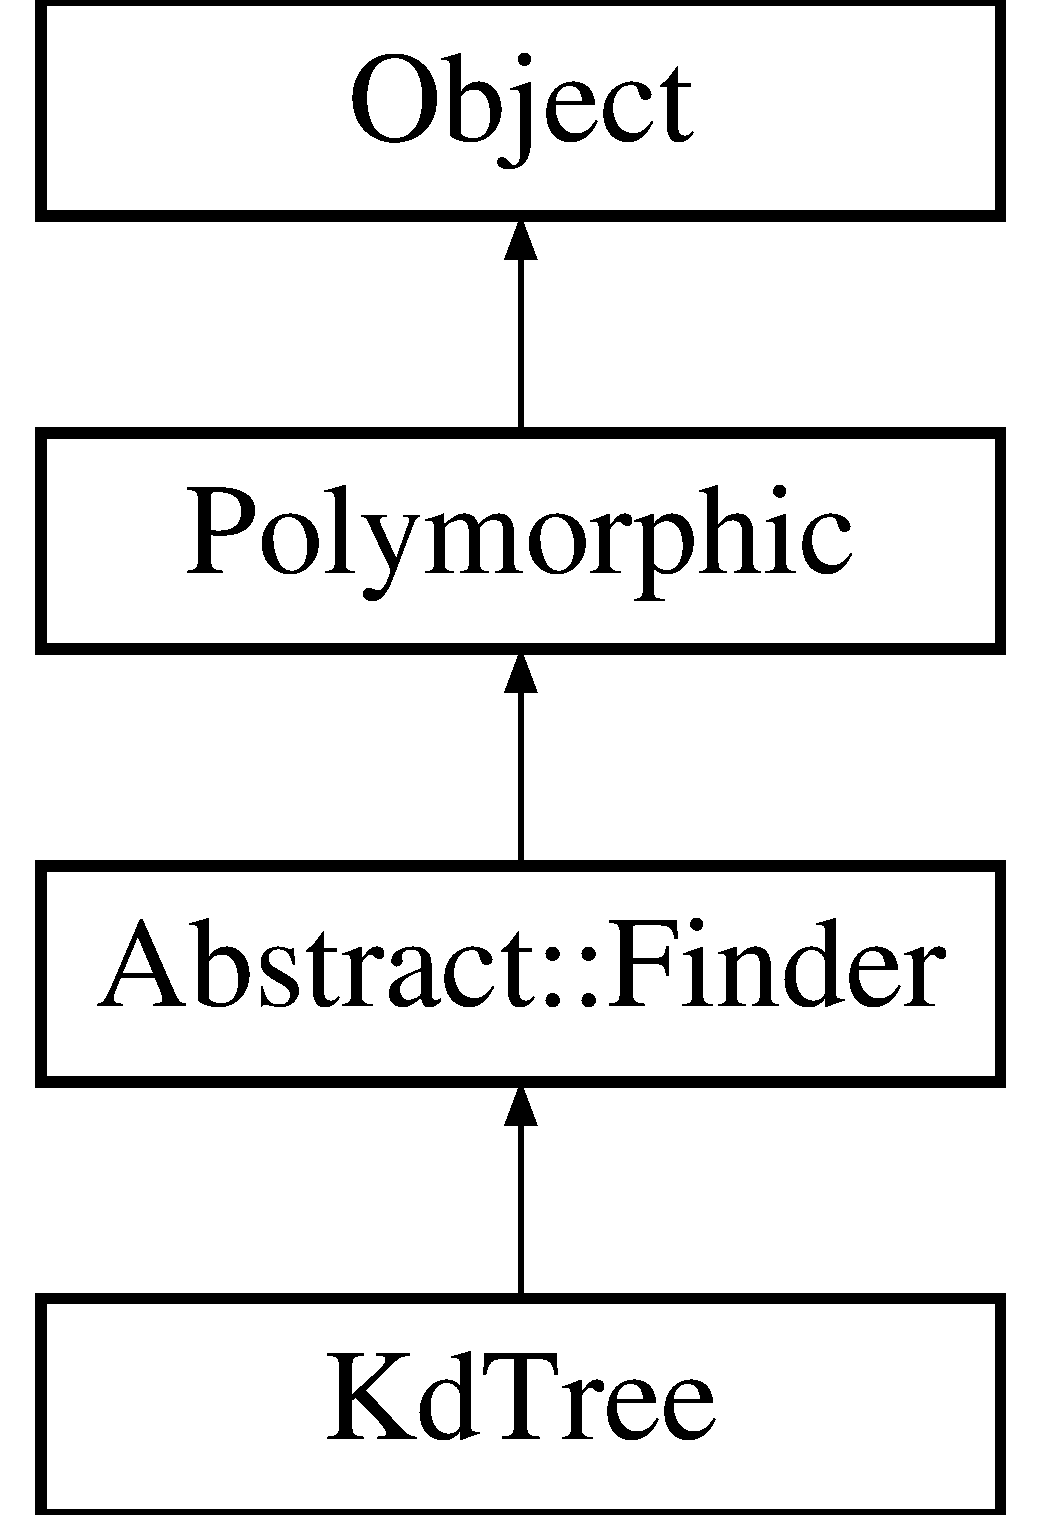
\includegraphics[height=4.000000cm]{classKdTree}
\end{center}
\end{figure}
\subsection*{Public Member Functions}
\begin{DoxyCompactItemize}
\item 
virtual int \hyperlink{classKdTree_a830840ce00b519f37e922a69733b68c1}{find\+Neighbours} (const int index, const Float radius, \hyperlink{classArray}{Array}$<$ \hyperlink{structNeighbourRecord}{Neighbour\+Record} $>$ \&neighbours, \hyperlink{classFlags}{Flags}$<$ Finder\+Flags $>$ flags=E\+M\+P\+T\+Y\+\_\+\+F\+L\+A\+GS, const Float error=0.\+\_\+f) const override
\end{DoxyCompactItemize}
\subsection*{Protected Member Functions}
\begin{DoxyCompactItemize}
\item 
\hypertarget{classKdTree_a2acc49e7949a6c0c2ba58a99cf2a1f63}{}\label{classKdTree_a2acc49e7949a6c0c2ba58a99cf2a1f63} 
virtual void {\bfseries build\+Impl} (\hyperlink{classArrayView}{Array\+View}$<$ \hyperlink{classBasicVector}{Vector} $>$ values) override
\end{DoxyCompactItemize}
\subsection*{Additional Inherited Members}


\subsection{Member Function Documentation}
\hypertarget{classKdTree_a830840ce00b519f37e922a69733b68c1}{}\label{classKdTree_a830840ce00b519f37e922a69733b68c1} 
\index{Kd\+Tree@{Kd\+Tree}!find\+Neighbours@{find\+Neighbours}}
\index{find\+Neighbours@{find\+Neighbours}!Kd\+Tree@{Kd\+Tree}}
\subsubsection{\texorpdfstring{find\+Neighbours()}{findNeighbours()}}
{\footnotesize\ttfamily virtual int Kd\+Tree\+::find\+Neighbours (\begin{DoxyParamCaption}\item[{const int}]{index,  }\item[{const Float}]{radius,  }\item[{\hyperlink{classArray}{Array}$<$ \hyperlink{structNeighbourRecord}{Neighbour\+Record} $>$ \&}]{neighbours,  }\item[{\hyperlink{classFlags}{Flags}$<$ Finder\+Flags $>$}]{flags = {\ttfamily EMPTY\+\_\+FLAGS},  }\item[{const Float}]{error = {\ttfamily 0.\+\_\+f} }\end{DoxyParamCaption}) const\hspace{0.3cm}{\ttfamily [inline]}, {\ttfamily [override]}, {\ttfamily [virtual]}}

Finds all points within given radius from a point. 
\begin{DoxyParams}{Parameters}
{\em point} & \\
\hline
{\em radius} & \\
\hline
{\em neighbours} & List of neighbours, as indices to the array \\
\hline
{\em error} & Approximate solution \\
\hline
\end{DoxyParams}
\begin{DoxyReturn}{Returns}
The number of neighbours. 
\end{DoxyReturn}
\begin{DoxyRefDesc}{Todo}
\item[\hyperlink{todo__todo000025}{Todo}]flags \end{DoxyRefDesc}


Implements \hyperlink{classAbstract_1_1Finder_a7f04b92d939992d0aa2978a259b2533f}{Abstract\+::\+Finder}.



The documentation for this class was generated from the following file\+:\begin{DoxyCompactItemize}
\item 
/home/pavel/projects/astro/sph2/src/tree/kdtree.\+h\end{DoxyCompactItemize}

\hypertarget{structSph_1_1KDTreeEigenMatrixAdaptor}{}\section{Sph\+:\+:K\+D\+Tree\+Eigen\+Matrix\+Adaptor$<$ Matrix\+Type, D\+IM, Distance $>$ Struct Template Reference}
\label{structSph_1_1KDTreeEigenMatrixAdaptor}\index{Sph\+::\+K\+D\+Tree\+Eigen\+Matrix\+Adaptor$<$ Matrix\+Type, D\+I\+M, Distance $>$@{Sph\+::\+K\+D\+Tree\+Eigen\+Matrix\+Adaptor$<$ Matrix\+Type, D\+I\+M, Distance $>$}}


{\ttfamily \#include $<$nanoflann.\+h$>$}

\subsection*{Public Types}
\begin{DoxyCompactItemize}
\item 
\hypertarget{structSph_1_1KDTreeEigenMatrixAdaptor_adacdae55d3f287c0bfd67524b0f1ae4c}{}\label{structSph_1_1KDTreeEigenMatrixAdaptor_adacdae55d3f287c0bfd67524b0f1ae4c} 
typedef \hyperlink{structSph_1_1KDTreeEigenMatrixAdaptor}{K\+D\+Tree\+Eigen\+Matrix\+Adaptor}$<$ Matrix\+Type, D\+IM, Distance $>$ {\bfseries self\+\_\+t}
\item 
\hypertarget{structSph_1_1KDTreeEigenMatrixAdaptor_ad578c10e7eccabf1feebda462881fb0a}{}\label{structSph_1_1KDTreeEigenMatrixAdaptor_ad578c10e7eccabf1feebda462881fb0a} 
typedef Matrix\+Type\+::\+Scalar {\bfseries num\+\_\+t}
\item 
\hypertarget{structSph_1_1KDTreeEigenMatrixAdaptor_a75133f75c59ed0607301a96d560c082a}{}\label{structSph_1_1KDTreeEigenMatrixAdaptor_a75133f75c59ed0607301a96d560c082a} 
typedef Matrix\+Type\+::\+Index {\bfseries Index\+Type}
\item 
\hypertarget{structSph_1_1KDTreeEigenMatrixAdaptor_aec2b2f7951d75aa359cf1d2c6823481c}{}\label{structSph_1_1KDTreeEigenMatrixAdaptor_aec2b2f7951d75aa359cf1d2c6823481c} 
typedef Distance\+::template traits$<$ num\+\_\+t, \hyperlink{structSph_1_1KDTreeEigenMatrixAdaptor}{self\+\_\+t} $>$\+::distance\+\_\+t {\bfseries metric\+\_\+t}
\item 
\hypertarget{structSph_1_1KDTreeEigenMatrixAdaptor_abdf6e5a32b79f2640eb982cdbaf321e5}{}\label{structSph_1_1KDTreeEigenMatrixAdaptor_abdf6e5a32b79f2640eb982cdbaf321e5} 
typedef \hyperlink{classSph_1_1KDTreeSingleIndexAdaptor}{K\+D\+Tree\+Single\+Index\+Adaptor}$<$ metric\+\_\+t, \hyperlink{structSph_1_1KDTreeEigenMatrixAdaptor}{self\+\_\+t}, D\+IM, Index\+Type $>$ {\bfseries index\+\_\+t}
\end{DoxyCompactItemize}
\subsection*{Public Member Functions}
\begin{DoxyCompactItemize}
\item 
\hyperlink{structSph_1_1KDTreeEigenMatrixAdaptor_a9968b3bdc08f148f419432a8339f1167}{K\+D\+Tree\+Eigen\+Matrix\+Adaptor} (const int dimensionality, const Matrix\+Type \&mat, const int leaf\+\_\+max\+\_\+size=10)
\begin{DoxyCompactList}\small\item\em The kd-\/tree index for the user to call its methods as usual with any other F\+L\+A\+NN index. \end{DoxyCompactList}\item 
void \hyperlink{structSph_1_1KDTreeEigenMatrixAdaptor_ae1335fbcb8f1189326409a1d582c6cb5}{query} (const num\+\_\+t $\ast$query\+\_\+point, const size\+\_\+t num\+\_\+closest, Index\+Type $\ast$out\+\_\+indices, num\+\_\+t $\ast$out\+\_\+distances\+\_\+sq, const int=10) const
\end{DoxyCompactItemize}
\begin{Indent}{\bf Interface expected by K\+D\+Tree\+Single\+Index\+Adaptor}\par
\begin{DoxyCompactItemize}
\item 
\hypertarget{structSph_1_1KDTreeEigenMatrixAdaptor_a29415a29d18e35f85a547607af77ff36}{}\label{structSph_1_1KDTreeEigenMatrixAdaptor_a29415a29d18e35f85a547607af77ff36} 
const \hyperlink{structSph_1_1KDTreeEigenMatrixAdaptor}{self\+\_\+t} \& {\bfseries derived} () const
\item 
\hypertarget{structSph_1_1KDTreeEigenMatrixAdaptor_a08ff232f37f98831214840241ce533b0}{}\label{structSph_1_1KDTreeEigenMatrixAdaptor_a08ff232f37f98831214840241ce533b0} 
\hyperlink{structSph_1_1KDTreeEigenMatrixAdaptor}{self\+\_\+t} \& {\bfseries derived} ()
\item 
\hypertarget{structSph_1_1KDTreeEigenMatrixAdaptor_a997746aa0357843f8f408f0606a14abe}{}\label{structSph_1_1KDTreeEigenMatrixAdaptor_a997746aa0357843f8f408f0606a14abe} 
size\+\_\+t {\bfseries kdtree\+\_\+get\+\_\+point\+\_\+count} () const
\item 
\hypertarget{structSph_1_1KDTreeEigenMatrixAdaptor_ad021e6fc3289c680fc0c6b0997903edd}{}\label{structSph_1_1KDTreeEigenMatrixAdaptor_ad021e6fc3289c680fc0c6b0997903edd} 
num\+\_\+t {\bfseries kdtree\+\_\+distance} (const num\+\_\+t $\ast$p1, const Index\+Type idx\+\_\+p2, Index\+Type size) const
\item 
\hypertarget{structSph_1_1KDTreeEigenMatrixAdaptor_aba83e56df76a23345da096f19d99dbd3}{}\label{structSph_1_1KDTreeEigenMatrixAdaptor_aba83e56df76a23345da096f19d99dbd3} 
num\+\_\+t {\bfseries kdtree\+\_\+get\+\_\+pt} (const Index\+Type idx, int dim) const
\item 
\hypertarget{structSph_1_1KDTreeEigenMatrixAdaptor_ae4c86f274b110668c318198af3d96897}{}\label{structSph_1_1KDTreeEigenMatrixAdaptor_ae4c86f274b110668c318198af3d96897} 
{\footnotesize template$<$class B\+B\+OX $>$ }\\bool {\bfseries kdtree\+\_\+get\+\_\+bbox} (B\+B\+OX \&) const
\end{DoxyCompactItemize}
\end{Indent}
\subsection*{Public Attributes}
\begin{DoxyCompactItemize}
\item 
\hypertarget{structSph_1_1KDTreeEigenMatrixAdaptor_a84e218145bfbdbb4b5eec2e4fd5c78f1}{}\label{structSph_1_1KDTreeEigenMatrixAdaptor_a84e218145bfbdbb4b5eec2e4fd5c78f1} 
\hyperlink{classSph_1_1KDTreeSingleIndexAdaptor}{index\+\_\+t} $\ast$ {\bfseries index}
\item 
\hypertarget{structSph_1_1KDTreeEigenMatrixAdaptor_ac56802ad9745e240e0885a6a3af6e597}{}\label{structSph_1_1KDTreeEigenMatrixAdaptor_ac56802ad9745e240e0885a6a3af6e597} 
const Matrix\+Type \& {\bfseries m\+\_\+data\+\_\+matrix}
\end{DoxyCompactItemize}


\subsection{Detailed Description}
\subsubsection*{template$<$class Matrix\+Type, int D\+IM = -\/1, class Distance = metric\+\_\+\+L2$>$\newline
struct Sph\+::\+K\+D\+Tree\+Eigen\+Matrix\+Adaptor$<$ Matrix\+Type, D\+I\+M, Distance $>$}

An L2-\/metric K\+D-\/tree adaptor for working with data directly stored in an Eigen \hyperlink{classMatrix}{Matrix}, without duplicating the data storage. Each row in the matrix represents a point in the state space.

Example of usage\+: 
\begin{DoxyCode}
Eigen::Matrix<num\_t,Dynamic,Dynamic>  mat;
\textcolor{comment}{// Fill out "mat"...}

\textcolor{keyword}{typedef} KDTreeEigenMatrixAdaptor< Eigen::Matrix<num\_t,Dynamic,Dynamic> >  my\_kd\_tree\_t;
\textcolor{keyword}{const} \textcolor{keywordtype}{int} max\_leaf = 10;
my\_kd\_tree\_t   mat\_index(dimdim, mat, max\_leaf );
mat\_index.index->buildIndex();
mat\_index.index->...
\end{DoxyCode}



\begin{DoxyTemplParams}{Template Parameters}
{\em D\+IM} & If set to $>$0, it specifies a compile-\/time fixed dimensionality for the points in the data set, allowing more compiler optimizations. \\
\hline
{\em Distance} & The distance metric to use\+: \hyperlink{structSph_1_1metric__L1}{metric\+\_\+\+L1}, \hyperlink{structSph_1_1metric__L2}{metric\+\_\+\+L2}, \hyperlink{structSph_1_1metric__L2__Simple}{metric\+\_\+\+L2\+\_\+\+Simple}, etc. \\
\hline
\end{DoxyTemplParams}


\subsection{Constructor \& Destructor Documentation}
\hypertarget{structSph_1_1KDTreeEigenMatrixAdaptor_a9968b3bdc08f148f419432a8339f1167}{}\label{structSph_1_1KDTreeEigenMatrixAdaptor_a9968b3bdc08f148f419432a8339f1167} 
\index{Sph\+::\+K\+D\+Tree\+Eigen\+Matrix\+Adaptor@{Sph\+::\+K\+D\+Tree\+Eigen\+Matrix\+Adaptor}!K\+D\+Tree\+Eigen\+Matrix\+Adaptor@{K\+D\+Tree\+Eigen\+Matrix\+Adaptor}}
\index{K\+D\+Tree\+Eigen\+Matrix\+Adaptor@{K\+D\+Tree\+Eigen\+Matrix\+Adaptor}!Sph\+::\+K\+D\+Tree\+Eigen\+Matrix\+Adaptor@{Sph\+::\+K\+D\+Tree\+Eigen\+Matrix\+Adaptor}}
\subsubsection{\texorpdfstring{K\+D\+Tree\+Eigen\+Matrix\+Adaptor()}{KDTreeEigenMatrixAdaptor()}}
{\footnotesize\ttfamily template$<$class Matrix\+Type , int D\+IM = -\/1, class Distance  = metric\+\_\+\+L2$>$ \\
\hyperlink{structSph_1_1KDTreeEigenMatrixAdaptor}{Sph\+::\+K\+D\+Tree\+Eigen\+Matrix\+Adaptor}$<$ Matrix\+Type, D\+IM, Distance $>$\+::\hyperlink{structSph_1_1KDTreeEigenMatrixAdaptor}{K\+D\+Tree\+Eigen\+Matrix\+Adaptor} (\begin{DoxyParamCaption}\item[{const int}]{dimensionality,  }\item[{const Matrix\+Type \&}]{mat,  }\item[{const int}]{leaf\+\_\+max\+\_\+size = {\ttfamily 10} }\end{DoxyParamCaption})\hspace{0.3cm}{\ttfamily [inline]}}



The kd-\/tree index for the user to call its methods as usual with any other F\+L\+A\+NN index. 

Constructor\+: takes a const ref to the matrix object with the data points 

\subsection{Member Function Documentation}
\hypertarget{structSph_1_1KDTreeEigenMatrixAdaptor_ae1335fbcb8f1189326409a1d582c6cb5}{}\label{structSph_1_1KDTreeEigenMatrixAdaptor_ae1335fbcb8f1189326409a1d582c6cb5} 
\index{Sph\+::\+K\+D\+Tree\+Eigen\+Matrix\+Adaptor@{Sph\+::\+K\+D\+Tree\+Eigen\+Matrix\+Adaptor}!query@{query}}
\index{query@{query}!Sph\+::\+K\+D\+Tree\+Eigen\+Matrix\+Adaptor@{Sph\+::\+K\+D\+Tree\+Eigen\+Matrix\+Adaptor}}
\subsubsection{\texorpdfstring{query()}{query()}}
{\footnotesize\ttfamily template$<$class Matrix\+Type , int D\+IM = -\/1, class Distance  = metric\+\_\+\+L2$>$ \\
void \hyperlink{structSph_1_1KDTreeEigenMatrixAdaptor}{Sph\+::\+K\+D\+Tree\+Eigen\+Matrix\+Adaptor}$<$ Matrix\+Type, D\+IM, Distance $>$\+::query (\begin{DoxyParamCaption}\item[{const num\+\_\+t $\ast$}]{query\+\_\+point,  }\item[{const size\+\_\+t}]{num\+\_\+closest,  }\item[{Index\+Type $\ast$}]{out\+\_\+indices,  }\item[{num\+\_\+t $\ast$}]{out\+\_\+distances\+\_\+sq,  }\item[{const int}]{ = {\ttfamily 10} }\end{DoxyParamCaption}) const\hspace{0.3cm}{\ttfamily [inline]}}

Query for the {\itshape num\+\_\+closest} closest points to a given point (entered as query\+\_\+point\mbox{[}0\+:dim-\/1\mbox{]}). Note that this is a short-\/cut method for index-\/$>$find\+Neighbors(). The user can also call index-\/$>$... methods as desired. \begin{DoxyNote}{Note}
n\+Checks\+\_\+\+I\+G\+N\+O\+R\+ED is ignored but kept for compatibility with the original F\+L\+A\+NN interface. 
\end{DoxyNote}


The documentation for this struct was generated from the following file\+:\begin{DoxyCompactItemize}
\item 
/home/pavel/projects/astro/sph2/src/tree/nanoflann.\+h\end{DoxyCompactItemize}

\hypertarget{classSph_1_1KDTreeSingleIndexAdaptor}{}\section{Sph\+:\+:K\+D\+Tree\+Single\+Index\+Adaptor$<$ Distance, Dataset\+Adaptor, D\+IM, Index\+Type $>$ Class Template Reference}
\label{classSph_1_1KDTreeSingleIndexAdaptor}\index{Sph\+::\+K\+D\+Tree\+Single\+Index\+Adaptor$<$ Distance, Dataset\+Adaptor, D\+I\+M, Index\+Type $>$@{Sph\+::\+K\+D\+Tree\+Single\+Index\+Adaptor$<$ Distance, Dataset\+Adaptor, D\+I\+M, Index\+Type $>$}}


{\ttfamily \#include $<$nanoflann.\+h$>$}

\subsection*{Classes}
\begin{DoxyCompactItemize}
\item 
struct \hyperlink{structSph_1_1KDTreeSingleIndexAdaptor_1_1Interval}{Interval}
\item 
struct \hyperlink{structSph_1_1KDTreeSingleIndexAdaptor_1_1Node}{Node}
\end{DoxyCompactItemize}
\subsection*{Public Types}
\begin{DoxyCompactItemize}
\item 
\hypertarget{classSph_1_1KDTreeSingleIndexAdaptor_ad953c11780c30bd9792ebef15777e4db}{}\label{classSph_1_1KDTreeSingleIndexAdaptor_ad953c11780c30bd9792ebef15777e4db} 
typedef Distance\+::\+Element\+Type {\bfseries Element\+Type}
\item 
\hypertarget{classSph_1_1KDTreeSingleIndexAdaptor_adaa73c70fe7b5a7087330090107cafba}{}\label{classSph_1_1KDTreeSingleIndexAdaptor_adaa73c70fe7b5a7087330090107cafba} 
typedef Distance\+::\+Distance\+Type {\bfseries Distance\+Type}
\end{DoxyCompactItemize}
\subsection*{Public Member Functions}
\begin{DoxyCompactItemize}
\item 
\hyperlink{classSph_1_1KDTreeSingleIndexAdaptor_a095fe85253e99a45f533ac830b7f69c3}{K\+D\+Tree\+Single\+Index\+Adaptor} (const int dimensionality, const Dataset\+Adaptor \&input\+Data, const \hyperlink{structSph_1_1KDTreeSingleIndexAdaptorParams}{K\+D\+Tree\+Single\+Index\+Adaptor\+Params} \&params=\hyperlink{structSph_1_1KDTreeSingleIndexAdaptorParams}{K\+D\+Tree\+Single\+Index\+Adaptor\+Params}())
\item 
\hyperlink{classSph_1_1KDTreeSingleIndexAdaptor_a809ad0ae1a688dd8f9870236a3157788}{$\sim$\+K\+D\+Tree\+Single\+Index\+Adaptor} ()
\item 
void \hyperlink{classSph_1_1KDTreeSingleIndexAdaptor_a977528560c451d99bc006f3a2084b0a4}{free\+Index} ()
\item 
void \hyperlink{classSph_1_1KDTreeSingleIndexAdaptor_a9806520fd7f6a35557d4c52043459358}{build\+Index} ()
\item 
size\+\_\+t \hyperlink{classSph_1_1KDTreeSingleIndexAdaptor_a48c011ca89a6a97693b7ba78e112d32c}{size} () const
\item 
size\+\_\+t \hyperlink{classSph_1_1KDTreeSingleIndexAdaptor_a3bdc53d8655e9e60c52fffc4fc4ce4dc}{veclen} () const
\item 
size\+\_\+t \hyperlink{classSph_1_1KDTreeSingleIndexAdaptor_a0f9d01c30153a3831103ba5381429e10}{used\+Memory} () const
\item 
void \hyperlink{classSph_1_1KDTreeSingleIndexAdaptor_adb51e3a0ffcdaf32a9153e82339070c1}{save\+Index} (F\+I\+LE $\ast$stream)
\item 
void \hyperlink{classSph_1_1KDTreeSingleIndexAdaptor_a0509f8a856bb3c6d278a182c5e6ce654}{load\+Index} (F\+I\+LE $\ast$stream)
\end{DoxyCompactItemize}
\begin{Indent}{\bf Query methods}\par
\begin{DoxyCompactItemize}
\item 
{\footnotesize template$<$typename R\+E\+S\+U\+L\+T\+S\+ET $>$ }\\bool \hyperlink{classSph_1_1KDTreeSingleIndexAdaptor_a444955d9248884e7fcb1fb238c3b0105}{find\+Neighbors} (R\+E\+S\+U\+L\+T\+S\+ET \&result, const \hyperlink{classBasicVector}{Vector} \&vec, const \hyperlink{structSph_1_1SearchParams}{Search\+Params} \&search\+Params) const
\item 
void \hyperlink{classSph_1_1KDTreeSingleIndexAdaptor_ab2712a5eafbf9344143d2eadff15e802}{knn\+Search} (const Element\+Type $\ast$query\+\_\+point, const size\+\_\+t num\+\_\+closest, Index\+Type $\ast$out\+\_\+indices, Distance\+Type $\ast$out\+\_\+distances\+\_\+sq, const int=10) const
\item 
size\+\_\+t \hyperlink{classSph_1_1KDTreeSingleIndexAdaptor_a1b00ad9bd5a4e2e265011ad4d2265e03}{radius\+Search} (const \hyperlink{classBasicVector}{Vector} \&query\+\_\+point, const Distance\+Type \&radius, \hyperlink{classArray}{Array}$<$ \hyperlink{structNeighbourRecord}{Neighbour\+Record} $>$ \&Indices\+Dists, const \hyperlink{structSph_1_1SearchParams}{Search\+Params} \&search\+Params) const
\item 
{\footnotesize template$<$class S\+E\+A\+R\+C\+H\+\_\+\+C\+A\+L\+L\+B\+A\+CK $>$ }\\size\+\_\+t \hyperlink{classSph_1_1KDTreeSingleIndexAdaptor_a536e60a78161542b81631f661635e7c5}{radius\+Search\+Custom\+Callback} (const \hyperlink{classBasicVector}{Vector} \&query\+\_\+point, S\+E\+A\+R\+C\+H\+\_\+\+C\+A\+L\+L\+B\+A\+CK \&result\+Set, const \hyperlink{structSph_1_1SearchParams}{Search\+Params} \&search\+Params=\hyperlink{structSph_1_1SearchParams}{Search\+Params}()) const
\end{DoxyCompactItemize}
\end{Indent}
\subsection*{Public Attributes}
\begin{DoxyCompactItemize}
\item 
\hypertarget{classSph_1_1KDTreeSingleIndexAdaptor_a5bfc663e833429c4f8c3761c50112139}{}\label{classSph_1_1KDTreeSingleIndexAdaptor_a5bfc663e833429c4f8c3761c50112139} 
Distance {\bfseries distance}
\end{DoxyCompactItemize}
\subsection*{Protected Types}
\begin{DoxyCompactItemize}
\item 
\hypertarget{classSph_1_1KDTreeSingleIndexAdaptor_a2916c59e8cd4645f22923be1286609c7}{}\label{classSph_1_1KDTreeSingleIndexAdaptor_a2916c59e8cd4645f22923be1286609c7} 
typedef \hyperlink{structSph_1_1KDTreeSingleIndexAdaptor_1_1Node}{Node} $\ast$ {\bfseries Node\+Ptr}
\item 
typedef \hyperlink{structSph_1_1array__or__vector__selector}{array\+\_\+or\+\_\+vector\+\_\+selector}$<$ D\+IM, \hyperlink{structSph_1_1KDTreeSingleIndexAdaptor_1_1Interval}{Interval} $>$\+::container\+\_\+t \hyperlink{classSph_1_1KDTreeSingleIndexAdaptor_aaf4a44f184e81388817dbffb5771f186}{Bounding\+Box}
\item 
typedef \hyperlink{structSph_1_1array__or__vector__selector}{array\+\_\+or\+\_\+vector\+\_\+selector}$<$ D\+IM, Distance\+Type $>$\+::container\+\_\+t \hyperlink{classSph_1_1KDTreeSingleIndexAdaptor_a662e739c535b91fc6a837595f00d28cb}{distance\+\_\+vector\+\_\+t}
\end{DoxyCompactItemize}
\subsection*{Protected Attributes}
\begin{DoxyCompactItemize}
\item 
\hyperlink{classArray}{Array}$<$ Index\+Type $>$ \hyperlink{classSph_1_1KDTreeSingleIndexAdaptor_a0a716f1a65f2d3f7984e8de05abae9ad}{vind}
\item 
\hypertarget{classSph_1_1KDTreeSingleIndexAdaptor_aee1c62c8fb9ccf4cd1f42984f32d6f7d}{}\label{classSph_1_1KDTreeSingleIndexAdaptor_aee1c62c8fb9ccf4cd1f42984f32d6f7d} 
size\+\_\+t {\bfseries m\+\_\+leaf\+\_\+max\+\_\+size}
\item 
const Dataset\+Adaptor \& \hyperlink{classSph_1_1KDTreeSingleIndexAdaptor_a4237e355ab2fc9487e0deb5bb96ad127}{dataset}
\begin{DoxyCompactList}\small\item\em The source of our data. \end{DoxyCompactList}\item 
\hypertarget{classSph_1_1KDTreeSingleIndexAdaptor_a194cf5399f404e46b10493481ee8b96c}{}\label{classSph_1_1KDTreeSingleIndexAdaptor_a194cf5399f404e46b10493481ee8b96c} 
const \hyperlink{structSph_1_1KDTreeSingleIndexAdaptorParams}{K\+D\+Tree\+Single\+Index\+Adaptor\+Params} {\bfseries index\+\_\+params}
\item 
\hypertarget{classSph_1_1KDTreeSingleIndexAdaptor_aa387d0a3ea9b0cff67c25acb488730a9}{}\label{classSph_1_1KDTreeSingleIndexAdaptor_aa387d0a3ea9b0cff67c25acb488730a9} 
size\+\_\+t \hyperlink{classSph_1_1KDTreeSingleIndexAdaptor_aa387d0a3ea9b0cff67c25acb488730a9}{m\+\_\+size}
\begin{DoxyCompactList}\small\item\em Number of current poins in the dataset. \end{DoxyCompactList}\item 
\hypertarget{classSph_1_1KDTreeSingleIndexAdaptor_aa6e68610be4a5763b02e36c77776543c}{}\label{classSph_1_1KDTreeSingleIndexAdaptor_aa6e68610be4a5763b02e36c77776543c} 
size\+\_\+t \hyperlink{classSph_1_1KDTreeSingleIndexAdaptor_aa6e68610be4a5763b02e36c77776543c}{m\+\_\+size\+\_\+at\+\_\+index\+\_\+build}
\begin{DoxyCompactList}\small\item\em Number of points in the dataset when the index was built. \end{DoxyCompactList}\item 
\hypertarget{classSph_1_1KDTreeSingleIndexAdaptor_a251cff804024c3de6cc015ac7628b9d5}{}\label{classSph_1_1KDTreeSingleIndexAdaptor_a251cff804024c3de6cc015ac7628b9d5} 
int \hyperlink{classSph_1_1KDTreeSingleIndexAdaptor_a251cff804024c3de6cc015ac7628b9d5}{dim}
\begin{DoxyCompactList}\small\item\em Dimensionality of each data point. \end{DoxyCompactList}\item 
\hyperlink{structSph_1_1KDTreeSingleIndexAdaptor_1_1Node}{Node\+Ptr} \hyperlink{classSph_1_1KDTreeSingleIndexAdaptor_ad50d49993d446a1ab158fc75d55a7bd5}{root\+\_\+node}
\item 
\hypertarget{classSph_1_1KDTreeSingleIndexAdaptor_a423451ae505e1bb392be569b897c8660}{}\label{classSph_1_1KDTreeSingleIndexAdaptor_a423451ae505e1bb392be569b897c8660} 
\hyperlink{classSph_1_1KDTreeSingleIndexAdaptor_aaf4a44f184e81388817dbffb5771f186}{Bounding\+Box} {\bfseries root\+\_\+bbox}
\item 
\hyperlink{classSph_1_1PooledAllocator}{Pooled\+Allocator} \hyperlink{classSph_1_1KDTreeSingleIndexAdaptor_a0c3283516e497df16563c3e635ae4d29}{pool}
\end{DoxyCompactItemize}


\subsection{Detailed Description}
\subsubsection*{template$<$typename Distance, class Dataset\+Adaptor, int D\+IM = -\/1, typename Index\+Type = size\+\_\+t$>$\newline
class Sph\+::\+K\+D\+Tree\+Single\+Index\+Adaptor$<$ Distance, Dataset\+Adaptor, D\+I\+M, Index\+Type $>$}

kd-\/tree index

Contains the k-\/d trees and other information for indexing a set of points for nearest-\/neighbor matching.

The class \char`\"{}\+Dataset\+Adaptor\char`\"{} must provide the following interface (can be non-\/virtual, inlined methods)\+:


\begin{DoxyCode}
      \textcolor{comment}{// Must return the number of data poins}
      \textcolor{keyword}{inline} \textcolor{keywordtype}{size\_t} kdtree\_get\_point\_count()\textcolor{keyword}{ const }\{ ... \}
   
      \textcolor{comment}{// [Only if using the metric\_L2\_Simple type] Must return the Euclidean (L2) distance between the}
vector \textcolor{stringliteral}{"p1[0:size-1]"} and the data point with index \textcolor{stringliteral}{"idx\_p2"} stored in the \textcolor{keyword}{class}:
      \textcolor{keyword}{inline} DistanceType kdtree\_distance(\textcolor{keyword}{const} T *p1, \textcolor{keyword}{const} \textcolor{keywordtype}{size\_t} idx\_p2,\textcolor{keywordtype}{size\_t} 
      \hyperlink{classSph_1_1KDTreeSingleIndexAdaptor_a48c011ca89a6a97693b7ba78e112d32c}{size})\textcolor{keyword}{ const }\{ ... \}
   
      \textcolor{comment}{// Must return the dim'th component of the idx'th point in the class:}
      \textcolor{keyword}{inline} T kdtree\_get\_pt(\textcolor{keyword}{const} \textcolor{keywordtype}{size\_t} idx, \textcolor{keywordtype}{int} \hyperlink{classSph_1_1KDTreeSingleIndexAdaptor_a251cff804024c3de6cc015ac7628b9d5}{dim})\textcolor{keyword}{ const }\{ ... \}
   
      \textcolor{comment}{// Optional bounding-box computation: return false to default to a standard bbox computation loop.}
      \textcolor{comment}{//   Return true if the BBOX was already computed by the class and returned in "bb" so it can be}
avoided to redo it again.
      \textcolor{comment}{//   Look at bb.size() to find out the expected dimensionality (e.g. 2 or 3 for point clouds)}
      \textcolor{keyword}{template} <\textcolor{keyword}{class} BBOX>
      \textcolor{keywordtype}{bool} kdtree\_get\_bbox(BBOX &bb)\textcolor{keyword}{ const}
\textcolor{keyword}{      }\{
         bb[0].low = ...; bb[0].high = ...;  \textcolor{comment}{// 0th dimension limits}
         bb[1].low = ...; bb[1].high = ...;  \textcolor{comment}{// 1st dimension limits}
         ...
         \textcolor{keywordflow}{return} \textcolor{keyword}{true};
      \}
\end{DoxyCode}



\begin{DoxyTemplParams}{Template Parameters}
{\em Dataset\+Adaptor} & The user-\/provided adaptor (see comments above). \\
\hline
{\em Distance} & The distance metric to use\+: \hyperlink{structSph_1_1metric__L1}{metric\+\_\+\+L1}, \hyperlink{structSph_1_1metric__L2}{metric\+\_\+\+L2}, \hyperlink{structSph_1_1metric__L2__Simple}{metric\+\_\+\+L2\+\_\+\+Simple}, etc. \\
\hline
{\em D\+IM} & Dimensionality of data points (e.\+g. 3 for 3D points) \\
\hline
{\em Index\+Type} & Will be typically size\+\_\+t or int \\
\hline
\end{DoxyTemplParams}


\subsection{Member Typedef Documentation}
\hypertarget{classSph_1_1KDTreeSingleIndexAdaptor_aaf4a44f184e81388817dbffb5771f186}{}\label{classSph_1_1KDTreeSingleIndexAdaptor_aaf4a44f184e81388817dbffb5771f186} 
\index{Sph\+::\+K\+D\+Tree\+Single\+Index\+Adaptor@{Sph\+::\+K\+D\+Tree\+Single\+Index\+Adaptor}!Bounding\+Box@{Bounding\+Box}}
\index{Bounding\+Box@{Bounding\+Box}!Sph\+::\+K\+D\+Tree\+Single\+Index\+Adaptor@{Sph\+::\+K\+D\+Tree\+Single\+Index\+Adaptor}}
\subsubsection{\texorpdfstring{Bounding\+Box}{BoundingBox}}
{\footnotesize\ttfamily template$<$typename Distance , class Dataset\+Adaptor , int D\+IM = -\/1, typename Index\+Type  = size\+\_\+t$>$ \\
typedef \hyperlink{structSph_1_1array__or__vector__selector}{array\+\_\+or\+\_\+vector\+\_\+selector}$<$D\+IM, \hyperlink{structSph_1_1KDTreeSingleIndexAdaptor_1_1Interval}{Interval}$>$\+::container\+\_\+t \hyperlink{classSph_1_1KDTreeSingleIndexAdaptor}{Sph\+::\+K\+D\+Tree\+Single\+Index\+Adaptor}$<$ Distance, Dataset\+Adaptor, D\+IM, Index\+Type $>$\+::\hyperlink{classSph_1_1KDTreeSingleIndexAdaptor_aaf4a44f184e81388817dbffb5771f186}{Bounding\+Box}\hspace{0.3cm}{\ttfamily [protected]}}

Define \char`\"{}\+Bounding\+Box\char`\"{} as a fixed-\/size or variable-\/size container depending on \char`\"{}\+D\+I\+M\char`\"{} \hypertarget{classSph_1_1KDTreeSingleIndexAdaptor_a662e739c535b91fc6a837595f00d28cb}{}\label{classSph_1_1KDTreeSingleIndexAdaptor_a662e739c535b91fc6a837595f00d28cb} 
\index{Sph\+::\+K\+D\+Tree\+Single\+Index\+Adaptor@{Sph\+::\+K\+D\+Tree\+Single\+Index\+Adaptor}!distance\+\_\+vector\+\_\+t@{distance\+\_\+vector\+\_\+t}}
\index{distance\+\_\+vector\+\_\+t@{distance\+\_\+vector\+\_\+t}!Sph\+::\+K\+D\+Tree\+Single\+Index\+Adaptor@{Sph\+::\+K\+D\+Tree\+Single\+Index\+Adaptor}}
\subsubsection{\texorpdfstring{distance\+\_\+vector\+\_\+t}{distance\_vector\_t}}
{\footnotesize\ttfamily template$<$typename Distance , class Dataset\+Adaptor , int D\+IM = -\/1, typename Index\+Type  = size\+\_\+t$>$ \\
typedef \hyperlink{structSph_1_1array__or__vector__selector}{array\+\_\+or\+\_\+vector\+\_\+selector}$<$D\+IM, Distance\+Type$>$\+::container\+\_\+t \hyperlink{classSph_1_1KDTreeSingleIndexAdaptor}{Sph\+::\+K\+D\+Tree\+Single\+Index\+Adaptor}$<$ Distance, Dataset\+Adaptor, D\+IM, Index\+Type $>$\+::\hyperlink{classSph_1_1KDTreeSingleIndexAdaptor_a662e739c535b91fc6a837595f00d28cb}{distance\+\_\+vector\+\_\+t}\hspace{0.3cm}{\ttfamily [protected]}}

Define \char`\"{}distance\+\_\+vector\+\_\+t\char`\"{} as a fixed-\/size or variable-\/size container depending on \char`\"{}\+D\+I\+M\char`\"{} 

\subsection{Constructor \& Destructor Documentation}
\hypertarget{classSph_1_1KDTreeSingleIndexAdaptor_a095fe85253e99a45f533ac830b7f69c3}{}\label{classSph_1_1KDTreeSingleIndexAdaptor_a095fe85253e99a45f533ac830b7f69c3} 
\index{Sph\+::\+K\+D\+Tree\+Single\+Index\+Adaptor@{Sph\+::\+K\+D\+Tree\+Single\+Index\+Adaptor}!K\+D\+Tree\+Single\+Index\+Adaptor@{K\+D\+Tree\+Single\+Index\+Adaptor}}
\index{K\+D\+Tree\+Single\+Index\+Adaptor@{K\+D\+Tree\+Single\+Index\+Adaptor}!Sph\+::\+K\+D\+Tree\+Single\+Index\+Adaptor@{Sph\+::\+K\+D\+Tree\+Single\+Index\+Adaptor}}
\subsubsection{\texorpdfstring{K\+D\+Tree\+Single\+Index\+Adaptor()}{KDTreeSingleIndexAdaptor()}}
{\footnotesize\ttfamily template$<$typename Distance , class Dataset\+Adaptor , int D\+IM = -\/1, typename Index\+Type  = size\+\_\+t$>$ \\
\hyperlink{classSph_1_1KDTreeSingleIndexAdaptor}{Sph\+::\+K\+D\+Tree\+Single\+Index\+Adaptor}$<$ Distance, Dataset\+Adaptor, D\+IM, Index\+Type $>$\+::\hyperlink{classSph_1_1KDTreeSingleIndexAdaptor}{K\+D\+Tree\+Single\+Index\+Adaptor} (\begin{DoxyParamCaption}\item[{const int}]{dimensionality,  }\item[{const Dataset\+Adaptor \&}]{input\+Data,  }\item[{const \hyperlink{structSph_1_1KDTreeSingleIndexAdaptorParams}{K\+D\+Tree\+Single\+Index\+Adaptor\+Params} \&}]{params = {\ttfamily \hyperlink{structSph_1_1KDTreeSingleIndexAdaptorParams}{K\+D\+Tree\+Single\+Index\+Adaptor\+Params}()} }\end{DoxyParamCaption})\hspace{0.3cm}{\ttfamily [inline]}}

K\+D\+Tree constructor

Refer to docs in R\+E\+A\+D\+M\+E.\+md or online in \href{https://github.com/jlblancoc/nanoflann}{\tt https\+://github.\+com/jlblancoc/nanoflann}

The K\+D-\/\+Tree point dimension (the length of each point in the datase, e.\+g. 3 for 3D points) is determined by means of\+:
\begin{DoxyItemize}
\item The {\itshape D\+IM} template parameter if $>$0 (highest priority)
\item Otherwise, the {\itshape dimensionality} parameter of this constructor.
\end{DoxyItemize}


\begin{DoxyParams}{Parameters}
{\em input\+Data} & Dataset with the input features \\
\hline
{\em params} & Basically, the maximum leaf node size \\
\hline
\end{DoxyParams}
\hypertarget{classSph_1_1KDTreeSingleIndexAdaptor_a809ad0ae1a688dd8f9870236a3157788}{}\label{classSph_1_1KDTreeSingleIndexAdaptor_a809ad0ae1a688dd8f9870236a3157788} 
\index{Sph\+::\+K\+D\+Tree\+Single\+Index\+Adaptor@{Sph\+::\+K\+D\+Tree\+Single\+Index\+Adaptor}!````~K\+D\+Tree\+Single\+Index\+Adaptor@{$\sim$\+K\+D\+Tree\+Single\+Index\+Adaptor}}
\index{````~K\+D\+Tree\+Single\+Index\+Adaptor@{$\sim$\+K\+D\+Tree\+Single\+Index\+Adaptor}!Sph\+::\+K\+D\+Tree\+Single\+Index\+Adaptor@{Sph\+::\+K\+D\+Tree\+Single\+Index\+Adaptor}}
\subsubsection{\texorpdfstring{$\sim$\+K\+D\+Tree\+Single\+Index\+Adaptor()}{~KDTreeSingleIndexAdaptor()}}
{\footnotesize\ttfamily template$<$typename Distance , class Dataset\+Adaptor , int D\+IM = -\/1, typename Index\+Type  = size\+\_\+t$>$ \\
\hyperlink{classSph_1_1KDTreeSingleIndexAdaptor}{Sph\+::\+K\+D\+Tree\+Single\+Index\+Adaptor}$<$ Distance, Dataset\+Adaptor, D\+IM, Index\+Type $>$\+::$\sim$\hyperlink{classSph_1_1KDTreeSingleIndexAdaptor}{K\+D\+Tree\+Single\+Index\+Adaptor} (\begin{DoxyParamCaption}{ }\end{DoxyParamCaption})\hspace{0.3cm}{\ttfamily [inline]}}

Standard destructor 

\subsection{Member Function Documentation}
\hypertarget{classSph_1_1KDTreeSingleIndexAdaptor_a9806520fd7f6a35557d4c52043459358}{}\label{classSph_1_1KDTreeSingleIndexAdaptor_a9806520fd7f6a35557d4c52043459358} 
\index{Sph\+::\+K\+D\+Tree\+Single\+Index\+Adaptor@{Sph\+::\+K\+D\+Tree\+Single\+Index\+Adaptor}!build\+Index@{build\+Index}}
\index{build\+Index@{build\+Index}!Sph\+::\+K\+D\+Tree\+Single\+Index\+Adaptor@{Sph\+::\+K\+D\+Tree\+Single\+Index\+Adaptor}}
\subsubsection{\texorpdfstring{build\+Index()}{buildIndex()}}
{\footnotesize\ttfamily template$<$typename Distance , class Dataset\+Adaptor , int D\+IM = -\/1, typename Index\+Type  = size\+\_\+t$>$ \\
void \hyperlink{classSph_1_1KDTreeSingleIndexAdaptor}{Sph\+::\+K\+D\+Tree\+Single\+Index\+Adaptor}$<$ Distance, Dataset\+Adaptor, D\+IM, Index\+Type $>$\+::build\+Index (\begin{DoxyParamCaption}{ }\end{DoxyParamCaption})\hspace{0.3cm}{\ttfamily [inline]}}

Builds the index \hypertarget{classSph_1_1KDTreeSingleIndexAdaptor_a444955d9248884e7fcb1fb238c3b0105}{}\label{classSph_1_1KDTreeSingleIndexAdaptor_a444955d9248884e7fcb1fb238c3b0105} 
\index{Sph\+::\+K\+D\+Tree\+Single\+Index\+Adaptor@{Sph\+::\+K\+D\+Tree\+Single\+Index\+Adaptor}!find\+Neighbors@{find\+Neighbors}}
\index{find\+Neighbors@{find\+Neighbors}!Sph\+::\+K\+D\+Tree\+Single\+Index\+Adaptor@{Sph\+::\+K\+D\+Tree\+Single\+Index\+Adaptor}}
\subsubsection{\texorpdfstring{find\+Neighbors()}{findNeighbors()}}
{\footnotesize\ttfamily template$<$typename Distance , class Dataset\+Adaptor , int D\+IM = -\/1, typename Index\+Type  = size\+\_\+t$>$ \\
template$<$typename R\+E\+S\+U\+L\+T\+S\+ET $>$ \\
bool \hyperlink{classSph_1_1KDTreeSingleIndexAdaptor}{Sph\+::\+K\+D\+Tree\+Single\+Index\+Adaptor}$<$ Distance, Dataset\+Adaptor, D\+IM, Index\+Type $>$\+::find\+Neighbors (\begin{DoxyParamCaption}\item[{R\+E\+S\+U\+L\+T\+S\+ET \&}]{result,  }\item[{const \hyperlink{classBasicVector}{Vector} \&}]{vec,  }\item[{const \hyperlink{structSph_1_1SearchParams}{Search\+Params} \&}]{search\+Params }\end{DoxyParamCaption}) const\hspace{0.3cm}{\ttfamily [inline]}}

Find set of nearest neighbors to vec\mbox{[}0\+:dim-\/1\mbox{]}. Their indices are stored inside the result object.

Params\+: result = the result object in which the indices of the nearest-\/neighbors are stored vec = the vector for which to search the nearest neighbors


\begin{DoxyTemplParams}{Template Parameters}
{\em R\+E\+S\+U\+L\+T\+S\+ET} & Should be any Result\+Set$<$\+Distance\+Type$>$ \\
\hline
\end{DoxyTemplParams}
\begin{DoxyReturn}{Returns}
True if the requested neighbors could be found. 
\end{DoxyReturn}
\begin{DoxySeeAlso}{See also}
\hyperlink{classSph_1_1KDTreeSingleIndexAdaptor_ab2712a5eafbf9344143d2eadff15e802}{knn\+Search}, \hyperlink{classSph_1_1KDTreeSingleIndexAdaptor_a1b00ad9bd5a4e2e265011ad4d2265e03}{radius\+Search} 
\end{DoxySeeAlso}
\hypertarget{classSph_1_1KDTreeSingleIndexAdaptor_a977528560c451d99bc006f3a2084b0a4}{}\label{classSph_1_1KDTreeSingleIndexAdaptor_a977528560c451d99bc006f3a2084b0a4} 
\index{Sph\+::\+K\+D\+Tree\+Single\+Index\+Adaptor@{Sph\+::\+K\+D\+Tree\+Single\+Index\+Adaptor}!free\+Index@{free\+Index}}
\index{free\+Index@{free\+Index}!Sph\+::\+K\+D\+Tree\+Single\+Index\+Adaptor@{Sph\+::\+K\+D\+Tree\+Single\+Index\+Adaptor}}
\subsubsection{\texorpdfstring{free\+Index()}{freeIndex()}}
{\footnotesize\ttfamily template$<$typename Distance , class Dataset\+Adaptor , int D\+IM = -\/1, typename Index\+Type  = size\+\_\+t$>$ \\
void \hyperlink{classSph_1_1KDTreeSingleIndexAdaptor}{Sph\+::\+K\+D\+Tree\+Single\+Index\+Adaptor}$<$ Distance, Dataset\+Adaptor, D\+IM, Index\+Type $>$\+::free\+Index (\begin{DoxyParamCaption}{ }\end{DoxyParamCaption})\hspace{0.3cm}{\ttfamily [inline]}}

Frees the previously-\/built index. Automatically called within \hyperlink{classSph_1_1KDTreeSingleIndexAdaptor_a9806520fd7f6a35557d4c52043459358}{build\+Index()}. \hypertarget{classSph_1_1KDTreeSingleIndexAdaptor_ab2712a5eafbf9344143d2eadff15e802}{}\label{classSph_1_1KDTreeSingleIndexAdaptor_ab2712a5eafbf9344143d2eadff15e802} 
\index{Sph\+::\+K\+D\+Tree\+Single\+Index\+Adaptor@{Sph\+::\+K\+D\+Tree\+Single\+Index\+Adaptor}!knn\+Search@{knn\+Search}}
\index{knn\+Search@{knn\+Search}!Sph\+::\+K\+D\+Tree\+Single\+Index\+Adaptor@{Sph\+::\+K\+D\+Tree\+Single\+Index\+Adaptor}}
\subsubsection{\texorpdfstring{knn\+Search()}{knnSearch()}}
{\footnotesize\ttfamily template$<$typename Distance , class Dataset\+Adaptor , int D\+IM = -\/1, typename Index\+Type  = size\+\_\+t$>$ \\
void \hyperlink{classSph_1_1KDTreeSingleIndexAdaptor}{Sph\+::\+K\+D\+Tree\+Single\+Index\+Adaptor}$<$ Distance, Dataset\+Adaptor, D\+IM, Index\+Type $>$\+::knn\+Search (\begin{DoxyParamCaption}\item[{const Element\+Type $\ast$}]{query\+\_\+point,  }\item[{const size\+\_\+t}]{num\+\_\+closest,  }\item[{Index\+Type $\ast$}]{out\+\_\+indices,  }\item[{Distance\+Type $\ast$}]{out\+\_\+distances\+\_\+sq,  }\item[{const int}]{ = {\ttfamily 10} }\end{DoxyParamCaption}) const\hspace{0.3cm}{\ttfamily [inline]}}

Find the \char`\"{}num\+\_\+closest\char`\"{} nearest neighbors to the {\itshape query\+\_\+point}\mbox{[}0\+:dim-\/1\mbox{]}. Their indices are stored inside the result object. \begin{DoxySeeAlso}{See also}
\hyperlink{classSph_1_1KDTreeSingleIndexAdaptor_a1b00ad9bd5a4e2e265011ad4d2265e03}{radius\+Search}, \hyperlink{classSph_1_1KDTreeSingleIndexAdaptor_a444955d9248884e7fcb1fb238c3b0105}{find\+Neighbors} 
\end{DoxySeeAlso}
\begin{DoxyNote}{Note}
n\+Checks\+\_\+\+I\+G\+N\+O\+R\+ED is ignored but kept for compatibility with the original F\+L\+A\+NN interface. 
\end{DoxyNote}
\hypertarget{classSph_1_1KDTreeSingleIndexAdaptor_a0509f8a856bb3c6d278a182c5e6ce654}{}\label{classSph_1_1KDTreeSingleIndexAdaptor_a0509f8a856bb3c6d278a182c5e6ce654} 
\index{Sph\+::\+K\+D\+Tree\+Single\+Index\+Adaptor@{Sph\+::\+K\+D\+Tree\+Single\+Index\+Adaptor}!load\+Index@{load\+Index}}
\index{load\+Index@{load\+Index}!Sph\+::\+K\+D\+Tree\+Single\+Index\+Adaptor@{Sph\+::\+K\+D\+Tree\+Single\+Index\+Adaptor}}
\subsubsection{\texorpdfstring{load\+Index()}{loadIndex()}}
{\footnotesize\ttfamily template$<$typename Distance , class Dataset\+Adaptor , int D\+IM = -\/1, typename Index\+Type  = size\+\_\+t$>$ \\
void \hyperlink{classSph_1_1KDTreeSingleIndexAdaptor}{Sph\+::\+K\+D\+Tree\+Single\+Index\+Adaptor}$<$ Distance, Dataset\+Adaptor, D\+IM, Index\+Type $>$\+::load\+Index (\begin{DoxyParamCaption}\item[{F\+I\+LE $\ast$}]{stream }\end{DoxyParamCaption})\hspace{0.3cm}{\ttfamily [inline]}}

Loads a previous index from a binary file. I\+M\+P\+O\+R\+T\+A\+NT N\+O\+TE\+: The set of data points is N\+OT stored in the file, so the index object must be constructed associated to the same source of data points used while building the index. See the example\+: examples/saveload\+\_\+example.\+cpp \begin{DoxySeeAlso}{See also}
\hyperlink{classSph_1_1KDTreeSingleIndexAdaptor_a0509f8a856bb3c6d278a182c5e6ce654}{load\+Index} 
\end{DoxySeeAlso}
\hypertarget{classSph_1_1KDTreeSingleIndexAdaptor_a1b00ad9bd5a4e2e265011ad4d2265e03}{}\label{classSph_1_1KDTreeSingleIndexAdaptor_a1b00ad9bd5a4e2e265011ad4d2265e03} 
\index{Sph\+::\+K\+D\+Tree\+Single\+Index\+Adaptor@{Sph\+::\+K\+D\+Tree\+Single\+Index\+Adaptor}!radius\+Search@{radius\+Search}}
\index{radius\+Search@{radius\+Search}!Sph\+::\+K\+D\+Tree\+Single\+Index\+Adaptor@{Sph\+::\+K\+D\+Tree\+Single\+Index\+Adaptor}}
\subsubsection{\texorpdfstring{radius\+Search()}{radiusSearch()}}
{\footnotesize\ttfamily template$<$typename Distance , class Dataset\+Adaptor , int D\+IM = -\/1, typename Index\+Type  = size\+\_\+t$>$ \\
size\+\_\+t \hyperlink{classSph_1_1KDTreeSingleIndexAdaptor}{Sph\+::\+K\+D\+Tree\+Single\+Index\+Adaptor}$<$ Distance, Dataset\+Adaptor, D\+IM, Index\+Type $>$\+::radius\+Search (\begin{DoxyParamCaption}\item[{const \hyperlink{classBasicVector}{Vector} \&}]{query\+\_\+point,  }\item[{const Distance\+Type \&}]{radius,  }\item[{\hyperlink{classArray}{Array}$<$ \hyperlink{structNeighbourRecord}{Neighbour\+Record} $>$ \&}]{Indices\+Dists,  }\item[{const \hyperlink{structSph_1_1SearchParams}{Search\+Params} \&}]{search\+Params }\end{DoxyParamCaption}) const\hspace{0.3cm}{\ttfamily [inline]}}

Find all the neighbors to {\itshape query\+\_\+point}\mbox{[}0\+:dim-\/1\mbox{]} within a maximum radius. The output is given as a vector of pairs, of which the first element is a point index and the second the corresponding distance. Previous contents of {\itshape Indices\+Dists} are cleared.

If search\+Params.\+sorted==true, the output list is sorted by ascending distances.

For a better performance, it is advisable to do a .reserve() on the vector if you have any wild guess about the number of expected matches.

\begin{DoxySeeAlso}{See also}
\hyperlink{classSph_1_1KDTreeSingleIndexAdaptor_ab2712a5eafbf9344143d2eadff15e802}{knn\+Search}, \hyperlink{classSph_1_1KDTreeSingleIndexAdaptor_a444955d9248884e7fcb1fb238c3b0105}{find\+Neighbors}, \hyperlink{classSph_1_1KDTreeSingleIndexAdaptor_a536e60a78161542b81631f661635e7c5}{radius\+Search\+Custom\+Callback} 
\end{DoxySeeAlso}
\begin{DoxyReturn}{Returns}
The number of points within the given radius (i.\+e. indices.\+size() or dists.\+size() ) 
\end{DoxyReturn}
\hypertarget{classSph_1_1KDTreeSingleIndexAdaptor_a536e60a78161542b81631f661635e7c5}{}\label{classSph_1_1KDTreeSingleIndexAdaptor_a536e60a78161542b81631f661635e7c5} 
\index{Sph\+::\+K\+D\+Tree\+Single\+Index\+Adaptor@{Sph\+::\+K\+D\+Tree\+Single\+Index\+Adaptor}!radius\+Search\+Custom\+Callback@{radius\+Search\+Custom\+Callback}}
\index{radius\+Search\+Custom\+Callback@{radius\+Search\+Custom\+Callback}!Sph\+::\+K\+D\+Tree\+Single\+Index\+Adaptor@{Sph\+::\+K\+D\+Tree\+Single\+Index\+Adaptor}}
\subsubsection{\texorpdfstring{radius\+Search\+Custom\+Callback()}{radiusSearchCustomCallback()}}
{\footnotesize\ttfamily template$<$typename Distance , class Dataset\+Adaptor , int D\+IM = -\/1, typename Index\+Type  = size\+\_\+t$>$ \\
template$<$class S\+E\+A\+R\+C\+H\+\_\+\+C\+A\+L\+L\+B\+A\+CK $>$ \\
size\+\_\+t \hyperlink{classSph_1_1KDTreeSingleIndexAdaptor}{Sph\+::\+K\+D\+Tree\+Single\+Index\+Adaptor}$<$ Distance, Dataset\+Adaptor, D\+IM, Index\+Type $>$\+::radius\+Search\+Custom\+Callback (\begin{DoxyParamCaption}\item[{const \hyperlink{classBasicVector}{Vector} \&}]{query\+\_\+point,  }\item[{S\+E\+A\+R\+C\+H\+\_\+\+C\+A\+L\+L\+B\+A\+CK \&}]{result\+Set,  }\item[{const \hyperlink{structSph_1_1SearchParams}{Search\+Params} \&}]{search\+Params = {\ttfamily \hyperlink{structSph_1_1SearchParams}{Search\+Params}()} }\end{DoxyParamCaption}) const\hspace{0.3cm}{\ttfamily [inline]}}

Just like \hyperlink{classSph_1_1KDTreeSingleIndexAdaptor_a1b00ad9bd5a4e2e265011ad4d2265e03}{radius\+Search()} but with a custom callback class for each point found in the radius of the query. See the source of Radius\+Result\+Set$<$$>$ as a start point for your own classes. \begin{DoxySeeAlso}{See also}
\hyperlink{classSph_1_1KDTreeSingleIndexAdaptor_a1b00ad9bd5a4e2e265011ad4d2265e03}{radius\+Search} 
\end{DoxySeeAlso}
\hypertarget{classSph_1_1KDTreeSingleIndexAdaptor_adb51e3a0ffcdaf32a9153e82339070c1}{}\label{classSph_1_1KDTreeSingleIndexAdaptor_adb51e3a0ffcdaf32a9153e82339070c1} 
\index{Sph\+::\+K\+D\+Tree\+Single\+Index\+Adaptor@{Sph\+::\+K\+D\+Tree\+Single\+Index\+Adaptor}!save\+Index@{save\+Index}}
\index{save\+Index@{save\+Index}!Sph\+::\+K\+D\+Tree\+Single\+Index\+Adaptor@{Sph\+::\+K\+D\+Tree\+Single\+Index\+Adaptor}}
\subsubsection{\texorpdfstring{save\+Index()}{saveIndex()}}
{\footnotesize\ttfamily template$<$typename Distance , class Dataset\+Adaptor , int D\+IM = -\/1, typename Index\+Type  = size\+\_\+t$>$ \\
void \hyperlink{classSph_1_1KDTreeSingleIndexAdaptor}{Sph\+::\+K\+D\+Tree\+Single\+Index\+Adaptor}$<$ Distance, Dataset\+Adaptor, D\+IM, Index\+Type $>$\+::save\+Index (\begin{DoxyParamCaption}\item[{F\+I\+LE $\ast$}]{stream }\end{DoxyParamCaption})\hspace{0.3cm}{\ttfamily [inline]}}

Stores the index in a binary file. I\+M\+P\+O\+R\+T\+A\+NT N\+O\+TE\+: The set of data points is N\+OT stored in the file, so when loading the index object it must be constructed associated to the same source of data points used while building it. See the example\+: examples/saveload\+\_\+example.\+cpp \begin{DoxySeeAlso}{See also}
\hyperlink{classSph_1_1KDTreeSingleIndexAdaptor_a0509f8a856bb3c6d278a182c5e6ce654}{load\+Index} 
\end{DoxySeeAlso}
\hypertarget{classSph_1_1KDTreeSingleIndexAdaptor_a48c011ca89a6a97693b7ba78e112d32c}{}\label{classSph_1_1KDTreeSingleIndexAdaptor_a48c011ca89a6a97693b7ba78e112d32c} 
\index{Sph\+::\+K\+D\+Tree\+Single\+Index\+Adaptor@{Sph\+::\+K\+D\+Tree\+Single\+Index\+Adaptor}!size@{size}}
\index{size@{size}!Sph\+::\+K\+D\+Tree\+Single\+Index\+Adaptor@{Sph\+::\+K\+D\+Tree\+Single\+Index\+Adaptor}}
\subsubsection{\texorpdfstring{size()}{size()}}
{\footnotesize\ttfamily template$<$typename Distance , class Dataset\+Adaptor , int D\+IM = -\/1, typename Index\+Type  = size\+\_\+t$>$ \\
size\+\_\+t \hyperlink{classSph_1_1KDTreeSingleIndexAdaptor}{Sph\+::\+K\+D\+Tree\+Single\+Index\+Adaptor}$<$ Distance, Dataset\+Adaptor, D\+IM, Index\+Type $>$\+::size (\begin{DoxyParamCaption}{ }\end{DoxyParamCaption}) const\hspace{0.3cm}{\ttfamily [inline]}}

Returns number of points in dataset \hypertarget{classSph_1_1KDTreeSingleIndexAdaptor_a0f9d01c30153a3831103ba5381429e10}{}\label{classSph_1_1KDTreeSingleIndexAdaptor_a0f9d01c30153a3831103ba5381429e10} 
\index{Sph\+::\+K\+D\+Tree\+Single\+Index\+Adaptor@{Sph\+::\+K\+D\+Tree\+Single\+Index\+Adaptor}!used\+Memory@{used\+Memory}}
\index{used\+Memory@{used\+Memory}!Sph\+::\+K\+D\+Tree\+Single\+Index\+Adaptor@{Sph\+::\+K\+D\+Tree\+Single\+Index\+Adaptor}}
\subsubsection{\texorpdfstring{used\+Memory()}{usedMemory()}}
{\footnotesize\ttfamily template$<$typename Distance , class Dataset\+Adaptor , int D\+IM = -\/1, typename Index\+Type  = size\+\_\+t$>$ \\
size\+\_\+t \hyperlink{classSph_1_1KDTreeSingleIndexAdaptor}{Sph\+::\+K\+D\+Tree\+Single\+Index\+Adaptor}$<$ Distance, Dataset\+Adaptor, D\+IM, Index\+Type $>$\+::used\+Memory (\begin{DoxyParamCaption}{ }\end{DoxyParamCaption}) const\hspace{0.3cm}{\ttfamily [inline]}}

Computes the inde memory usage Returns\+: memory used by the index \hypertarget{classSph_1_1KDTreeSingleIndexAdaptor_a3bdc53d8655e9e60c52fffc4fc4ce4dc}{}\label{classSph_1_1KDTreeSingleIndexAdaptor_a3bdc53d8655e9e60c52fffc4fc4ce4dc} 
\index{Sph\+::\+K\+D\+Tree\+Single\+Index\+Adaptor@{Sph\+::\+K\+D\+Tree\+Single\+Index\+Adaptor}!veclen@{veclen}}
\index{veclen@{veclen}!Sph\+::\+K\+D\+Tree\+Single\+Index\+Adaptor@{Sph\+::\+K\+D\+Tree\+Single\+Index\+Adaptor}}
\subsubsection{\texorpdfstring{veclen()}{veclen()}}
{\footnotesize\ttfamily template$<$typename Distance , class Dataset\+Adaptor , int D\+IM = -\/1, typename Index\+Type  = size\+\_\+t$>$ \\
size\+\_\+t \hyperlink{classSph_1_1KDTreeSingleIndexAdaptor}{Sph\+::\+K\+D\+Tree\+Single\+Index\+Adaptor}$<$ Distance, Dataset\+Adaptor, D\+IM, Index\+Type $>$\+::veclen (\begin{DoxyParamCaption}{ }\end{DoxyParamCaption}) const\hspace{0.3cm}{\ttfamily [inline]}}

Returns the length of each point in the dataset 

\subsection{Member Data Documentation}
\hypertarget{classSph_1_1KDTreeSingleIndexAdaptor_a4237e355ab2fc9487e0deb5bb96ad127}{}\label{classSph_1_1KDTreeSingleIndexAdaptor_a4237e355ab2fc9487e0deb5bb96ad127} 
\index{Sph\+::\+K\+D\+Tree\+Single\+Index\+Adaptor@{Sph\+::\+K\+D\+Tree\+Single\+Index\+Adaptor}!dataset@{dataset}}
\index{dataset@{dataset}!Sph\+::\+K\+D\+Tree\+Single\+Index\+Adaptor@{Sph\+::\+K\+D\+Tree\+Single\+Index\+Adaptor}}
\subsubsection{\texorpdfstring{dataset}{dataset}}
{\footnotesize\ttfamily template$<$typename Distance , class Dataset\+Adaptor , int D\+IM = -\/1, typename Index\+Type  = size\+\_\+t$>$ \\
const Dataset\+Adaptor\& \hyperlink{classSph_1_1KDTreeSingleIndexAdaptor}{Sph\+::\+K\+D\+Tree\+Single\+Index\+Adaptor}$<$ Distance, Dataset\+Adaptor, D\+IM, Index\+Type $>$\+::dataset\hspace{0.3cm}{\ttfamily [protected]}}



The source of our data. 

The dataset used by this index \hypertarget{classSph_1_1KDTreeSingleIndexAdaptor_a0c3283516e497df16563c3e635ae4d29}{}\label{classSph_1_1KDTreeSingleIndexAdaptor_a0c3283516e497df16563c3e635ae4d29} 
\index{Sph\+::\+K\+D\+Tree\+Single\+Index\+Adaptor@{Sph\+::\+K\+D\+Tree\+Single\+Index\+Adaptor}!pool@{pool}}
\index{pool@{pool}!Sph\+::\+K\+D\+Tree\+Single\+Index\+Adaptor@{Sph\+::\+K\+D\+Tree\+Single\+Index\+Adaptor}}
\subsubsection{\texorpdfstring{pool}{pool}}
{\footnotesize\ttfamily template$<$typename Distance , class Dataset\+Adaptor , int D\+IM = -\/1, typename Index\+Type  = size\+\_\+t$>$ \\
\hyperlink{classSph_1_1PooledAllocator}{Pooled\+Allocator} \hyperlink{classSph_1_1KDTreeSingleIndexAdaptor}{Sph\+::\+K\+D\+Tree\+Single\+Index\+Adaptor}$<$ Distance, Dataset\+Adaptor, D\+IM, Index\+Type $>$\+::pool\hspace{0.3cm}{\ttfamily [protected]}}

Pooled memory allocator.

Using a pooled memory allocator is more efficient than allocating memory directly when there is a large number small of memory allocations. \hypertarget{classSph_1_1KDTreeSingleIndexAdaptor_ad50d49993d446a1ab158fc75d55a7bd5}{}\label{classSph_1_1KDTreeSingleIndexAdaptor_ad50d49993d446a1ab158fc75d55a7bd5} 
\index{Sph\+::\+K\+D\+Tree\+Single\+Index\+Adaptor@{Sph\+::\+K\+D\+Tree\+Single\+Index\+Adaptor}!root\+\_\+node@{root\+\_\+node}}
\index{root\+\_\+node@{root\+\_\+node}!Sph\+::\+K\+D\+Tree\+Single\+Index\+Adaptor@{Sph\+::\+K\+D\+Tree\+Single\+Index\+Adaptor}}
\subsubsection{\texorpdfstring{root\+\_\+node}{root\_node}}
{\footnotesize\ttfamily template$<$typename Distance , class Dataset\+Adaptor , int D\+IM = -\/1, typename Index\+Type  = size\+\_\+t$>$ \\
\hyperlink{structSph_1_1KDTreeSingleIndexAdaptor_1_1Node}{Node\+Ptr} \hyperlink{classSph_1_1KDTreeSingleIndexAdaptor}{Sph\+::\+K\+D\+Tree\+Single\+Index\+Adaptor}$<$ Distance, Dataset\+Adaptor, D\+IM, Index\+Type $>$\+::root\+\_\+node\hspace{0.3cm}{\ttfamily [protected]}}

The K\+D-\/tree used to find neighbours \hypertarget{classSph_1_1KDTreeSingleIndexAdaptor_a0a716f1a65f2d3f7984e8de05abae9ad}{}\label{classSph_1_1KDTreeSingleIndexAdaptor_a0a716f1a65f2d3f7984e8de05abae9ad} 
\index{Sph\+::\+K\+D\+Tree\+Single\+Index\+Adaptor@{Sph\+::\+K\+D\+Tree\+Single\+Index\+Adaptor}!vind@{vind}}
\index{vind@{vind}!Sph\+::\+K\+D\+Tree\+Single\+Index\+Adaptor@{Sph\+::\+K\+D\+Tree\+Single\+Index\+Adaptor}}
\subsubsection{\texorpdfstring{vind}{vind}}
{\footnotesize\ttfamily template$<$typename Distance , class Dataset\+Adaptor , int D\+IM = -\/1, typename Index\+Type  = size\+\_\+t$>$ \\
\hyperlink{classArray}{Array}$<$Index\+Type$>$ \hyperlink{classSph_1_1KDTreeSingleIndexAdaptor}{Sph\+::\+K\+D\+Tree\+Single\+Index\+Adaptor}$<$ Distance, Dataset\+Adaptor, D\+IM, Index\+Type $>$\+::vind\hspace{0.3cm}{\ttfamily [protected]}}

\hyperlink{classArray}{Array} of indices to vectors in the dataset. 

The documentation for this class was generated from the following file\+:\begin{DoxyCompactItemize}
\item 
/home/pavel/projects/astro/sph2/src/tree/nanoflann.\+h\end{DoxyCompactItemize}

\hypertarget{structSph_1_1KDTreeSingleIndexAdaptorParams}{}\section{Sph\+:\+:K\+D\+Tree\+Single\+Index\+Adaptor\+Params Struct Reference}
\label{structSph_1_1KDTreeSingleIndexAdaptorParams}\index{Sph\+::\+K\+D\+Tree\+Single\+Index\+Adaptor\+Params@{Sph\+::\+K\+D\+Tree\+Single\+Index\+Adaptor\+Params}}


{\ttfamily \#include $<$nanoflann.\+h$>$}

\subsection*{Public Member Functions}
\begin{DoxyCompactItemize}
\item 
\hypertarget{structSph_1_1KDTreeSingleIndexAdaptorParams_afd2be3b33dd16f91d49418319f099d03}{}\label{structSph_1_1KDTreeSingleIndexAdaptorParams_afd2be3b33dd16f91d49418319f099d03} 
{\bfseries K\+D\+Tree\+Single\+Index\+Adaptor\+Params} (size\+\_\+t \+\_\+leaf\+\_\+max\+\_\+size=10)
\end{DoxyCompactItemize}
\subsection*{Public Attributes}
\begin{DoxyCompactItemize}
\item 
\hypertarget{structSph_1_1KDTreeSingleIndexAdaptorParams_a46daa5c75e4141b14ada18f6180cb2dc}{}\label{structSph_1_1KDTreeSingleIndexAdaptorParams_a46daa5c75e4141b14ada18f6180cb2dc} 
size\+\_\+t {\bfseries leaf\+\_\+max\+\_\+size}
\end{DoxyCompactItemize}


\subsection{Detailed Description}
Parameters (see R\+E\+A\+D\+M\+E.\+md) 

The documentation for this struct was generated from the following file\+:\begin{DoxyCompactItemize}
\item 
/home/pavel/projects/astro/sph2/src/tree/nanoflann.\+h\end{DoxyCompactItemize}

\hypertarget{classKernel}{}\section{Kernel$<$ T\+Derived $>$ Class Template Reference}
\label{classKernel}\index{Kernel$<$ T\+Derived $>$@{Kernel$<$ T\+Derived $>$}}


{\ttfamily \#include $<$kernel.\+h$>$}

Inheritance diagram for Kernel$<$ T\+Derived $>$\+:\begin{figure}[H]
\begin{center}
\leavevmode
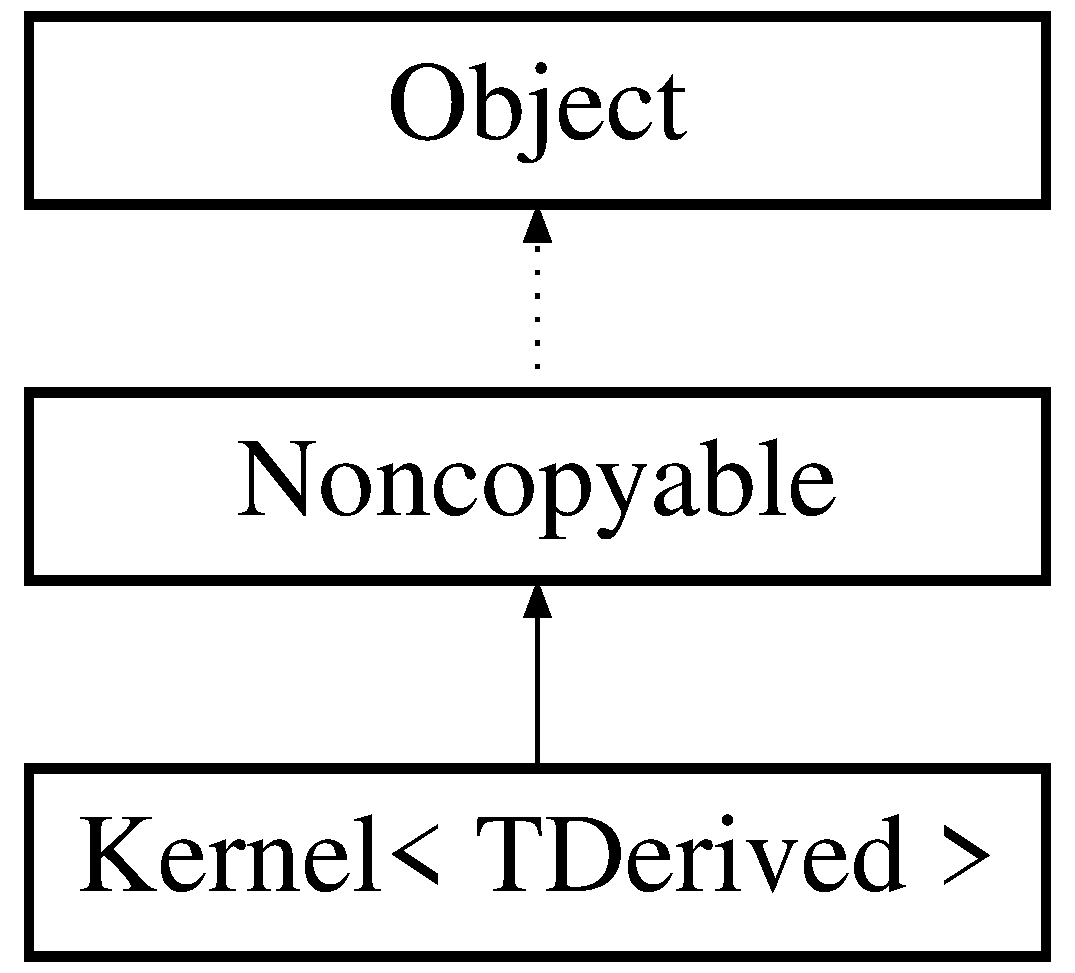
\includegraphics[height=3.000000cm]{classKernel}
\end{center}
\end{figure}
\subsection*{Public Member Functions}
\begin{DoxyCompactItemize}
\item 
I\+N\+L\+I\+NE Float \hyperlink{classKernel_aa8b9718f58edb6353460653f61b28131}{value} (const \hyperlink{classBasicVector}{Vector} \&r, const Float \&h) const
\item 
\hypertarget{classKernel_af6bb7a4aafc292cfca4225f2c6150509}{}\label{classKernel_af6bb7a4aafc292cfca4225f2c6150509} 
I\+N\+L\+I\+NE \hyperlink{classBasicVector}{Vector} {\bfseries grad} (const \hyperlink{classBasicVector}{Vector} \&r, const Float \&h) const
\end{DoxyCompactItemize}


\subsection{Detailed Description}
\subsubsection*{template$<$class T\+Derived$>$\newline
class Kernel$<$ T\+Derived $>$}

A base class for all S\+PH kernels, providing interface for computing kernel values and gradients. All derived class must implement method {\ttfamily value} and {\ttfamily grad}. Both function take S\+Q\+U\+A\+R\+ED value of dimensionless distance q as a parameter. Function value returns the kernel value, grad returns gradient D\+I\+V\+I\+D\+ED BY q. 

\subsection{Member Function Documentation}
\hypertarget{classKernel_aa8b9718f58edb6353460653f61b28131}{}\label{classKernel_aa8b9718f58edb6353460653f61b28131} 
\index{Kernel@{Kernel}!value@{value}}
\index{value@{value}!Kernel@{Kernel}}
\subsubsection{\texorpdfstring{value()}{value()}}
{\footnotesize\ttfamily template$<$class T\+Derived$>$ \\
I\+N\+L\+I\+NE Float \hyperlink{classKernel}{Kernel}$<$ T\+Derived $>$\+::value (\begin{DoxyParamCaption}\item[{const \hyperlink{classBasicVector}{Vector} \&}]{r,  }\item[{const Float \&}]{h }\end{DoxyParamCaption}) const\hspace{0.3cm}{\ttfamily [inline]}}

Value of kernel at given point this should be called only once for a pair of particles as there is expensive division \begin{DoxyRefDesc}{Todo}
\item[\hyperlink{todo__todo000016}{Todo}]Test this carefully before going any further 

Potentially precompute the 3rd power ... 

How to resolve dimensions for d!=3 ?? \end{DoxyRefDesc}


The documentation for this class was generated from the following file\+:\begin{DoxyCompactItemize}
\item 
/home/pavel/projects/astro/sph2/src/kernel/kernel.\+h\end{DoxyCompactItemize}

\hypertarget{classSph_1_1KNNResultSet}{}\section{Sph\+:\+:K\+N\+N\+Result\+Set$<$ Distance\+Type, Index\+Type, Count\+Type $>$ Class Template Reference}
\label{classSph_1_1KNNResultSet}\index{Sph\+::\+K\+N\+N\+Result\+Set$<$ Distance\+Type, Index\+Type, Count\+Type $>$@{Sph\+::\+K\+N\+N\+Result\+Set$<$ Distance\+Type, Index\+Type, Count\+Type $>$}}
\subsection*{Public Member Functions}
\begin{DoxyCompactItemize}
\item 
\hypertarget{classSph_1_1KNNResultSet_a6ae179eab65d9be310ff80a9157f5e68}{}\label{classSph_1_1KNNResultSet_a6ae179eab65d9be310ff80a9157f5e68} 
{\bfseries K\+N\+N\+Result\+Set} (Count\+Type capacity\+\_\+)
\item 
\hypertarget{classSph_1_1KNNResultSet_a98d885efb9616640bd806b7cdb238846}{}\label{classSph_1_1KNNResultSet_a98d885efb9616640bd806b7cdb238846} 
void {\bfseries init} (Index\+Type $\ast$indices\+\_\+, Distance\+Type $\ast$dists\+\_\+)
\item 
\hypertarget{classSph_1_1KNNResultSet_a71008c4c8d17e64d6976ee852036c6de}{}\label{classSph_1_1KNNResultSet_a71008c4c8d17e64d6976ee852036c6de} 
Count\+Type {\bfseries size} () const
\item 
\hypertarget{classSph_1_1KNNResultSet_a026d995c0a228dbc1c322d8977fab5b0}{}\label{classSph_1_1KNNResultSet_a026d995c0a228dbc1c322d8977fab5b0} 
bool {\bfseries full} () const
\item 
\hypertarget{classSph_1_1KNNResultSet_a2ad6b553ca851a29ba007f6b2e4f1074}{}\label{classSph_1_1KNNResultSet_a2ad6b553ca851a29ba007f6b2e4f1074} 
void {\bfseries add\+Point} (Distance\+Type dist, Index\+Type index)
\item 
\hypertarget{classSph_1_1KNNResultSet_a99836c91ab02516ce91b45f49301adf5}{}\label{classSph_1_1KNNResultSet_a99836c91ab02516ce91b45f49301adf5} 
Distance\+Type {\bfseries worst\+Dist} () const
\end{DoxyCompactItemize}


The documentation for this class was generated from the following file\+:\begin{DoxyCompactItemize}
\item 
/home/pavel/projects/astro/sph2/src/tree/nanoflann.\+h\end{DoxyCompactItemize}

\hypertarget{structSph_1_1L1__Adaptor}{}\section{Sph\+:\+:L1\+\_\+\+Adaptor$<$ T, Data\+Source, \+\_\+\+Distance\+Type $>$ Struct Template Reference}
\label{structSph_1_1L1__Adaptor}\index{Sph\+::\+L1\+\_\+\+Adaptor$<$ T, Data\+Source, \+\_\+\+Distance\+Type $>$@{Sph\+::\+L1\+\_\+\+Adaptor$<$ T, Data\+Source, \+\_\+\+Distance\+Type $>$}}


{\ttfamily \#include $<$nanoflann.\+h$>$}

\subsection*{Public Types}
\begin{DoxyCompactItemize}
\item 
\hypertarget{structSph_1_1L1__Adaptor_a6deb0201338f2110e1eae879a884edbb}{}\label{structSph_1_1L1__Adaptor_a6deb0201338f2110e1eae879a884edbb} 
typedef T {\bfseries Element\+Type}
\item 
\hypertarget{structSph_1_1L1__Adaptor_a3c106e0998983a06a7b2789cb5d8d479}{}\label{structSph_1_1L1__Adaptor_a3c106e0998983a06a7b2789cb5d8d479} 
typedef \+\_\+\+Distance\+Type {\bfseries Distance\+Type}
\end{DoxyCompactItemize}
\subsection*{Public Member Functions}
\begin{DoxyCompactItemize}
\item 
\hypertarget{structSph_1_1L1__Adaptor_a69ec3a85eadd3533e8d2c0e614852f73}{}\label{structSph_1_1L1__Adaptor_a69ec3a85eadd3533e8d2c0e614852f73} 
{\bfseries L1\+\_\+\+Adaptor} (const Data\+Source \&\+\_\+data\+\_\+source)
\item 
\hypertarget{structSph_1_1L1__Adaptor_a76be53fb089b9aa63d523de66dae2f29}{}\label{structSph_1_1L1__Adaptor_a76be53fb089b9aa63d523de66dae2f29} 
Distance\+Type {\bfseries operator()} (const T $\ast$a, const size\+\_\+t b\+\_\+idx, size\+\_\+t size, Distance\+Type worst\+\_\+dist=-\/1) const
\item 
\hypertarget{structSph_1_1L1__Adaptor_ad1f49f13b3756278720413e0cd6a0833}{}\label{structSph_1_1L1__Adaptor_ad1f49f13b3756278720413e0cd6a0833} 
{\footnotesize template$<$typename U , typename V $>$ }\\Distance\+Type {\bfseries accum\+\_\+dist} (const U a, const V b, int) const
\end{DoxyCompactItemize}
\subsection*{Public Attributes}
\begin{DoxyCompactItemize}
\item 
\hypertarget{structSph_1_1L1__Adaptor_a6d97126b0f1ae1a7fe18345937c1ecfb}{}\label{structSph_1_1L1__Adaptor_a6d97126b0f1ae1a7fe18345937c1ecfb} 
const Data\+Source \& {\bfseries data\+\_\+source}
\end{DoxyCompactItemize}


\subsection{Detailed Description}
\subsubsection*{template$<$class T, class Data\+Source, typename \+\_\+\+Distance\+Type = T$>$\newline
struct Sph\+::\+L1\+\_\+\+Adaptor$<$ T, Data\+Source, \+\_\+\+Distance\+Type $>$}

Manhattan distance functor (generic version, optimized for high-\/dimensionality data sets). Corresponding distance traits\+: \hyperlink{structSph_1_1metric__L1}{metric\+\_\+\+L1} 
\begin{DoxyTemplParams}{Template Parameters}
{\em T} & Type of the elements (e.\+g. double, float, uint8\+\_\+t) \\
\hline
{\em \+\_\+\+Distance\+Type} & Type of distance variables (must be signed) (e.\+g. float, double, int64\+\_\+t) \\
\hline
\end{DoxyTemplParams}


The documentation for this struct was generated from the following file\+:\begin{DoxyCompactItemize}
\item 
/home/pavel/projects/astro/sph2/src/tree/nanoflann.\+h\end{DoxyCompactItemize}

\hypertarget{structSph_1_1L2__Adaptor}{}\section{Sph\+:\+:L2\+\_\+\+Adaptor$<$ T, Data\+Source, \+\_\+\+Distance\+Type $>$ Struct Template Reference}
\label{structSph_1_1L2__Adaptor}\index{Sph\+::\+L2\+\_\+\+Adaptor$<$ T, Data\+Source, \+\_\+\+Distance\+Type $>$@{Sph\+::\+L2\+\_\+\+Adaptor$<$ T, Data\+Source, \+\_\+\+Distance\+Type $>$}}


{\ttfamily \#include $<$nanoflann.\+h$>$}

\subsection*{Public Types}
\begin{DoxyCompactItemize}
\item 
\hypertarget{structSph_1_1L2__Adaptor_a8ea959f5cbbd6a82995ca45f2057c7c4}{}\label{structSph_1_1L2__Adaptor_a8ea959f5cbbd6a82995ca45f2057c7c4} 
typedef T {\bfseries Element\+Type}
\item 
\hypertarget{structSph_1_1L2__Adaptor_a65e7df910b606d8aceb0266da3b10116}{}\label{structSph_1_1L2__Adaptor_a65e7df910b606d8aceb0266da3b10116} 
typedef \+\_\+\+Distance\+Type {\bfseries Distance\+Type}
\end{DoxyCompactItemize}
\subsection*{Public Member Functions}
\begin{DoxyCompactItemize}
\item 
\hypertarget{structSph_1_1L2__Adaptor_a78f6f6594fc4a3275554ae233c3efa6a}{}\label{structSph_1_1L2__Adaptor_a78f6f6594fc4a3275554ae233c3efa6a} 
{\bfseries L2\+\_\+\+Adaptor} (const Data\+Source \&\+\_\+data\+\_\+source)
\item 
\hypertarget{structSph_1_1L2__Adaptor_a0196461da1415c227e3223f81e64cb4f}{}\label{structSph_1_1L2__Adaptor_a0196461da1415c227e3223f81e64cb4f} 
Distance\+Type {\bfseries operator()} (const T $\ast$a, const size\+\_\+t b\+\_\+idx, size\+\_\+t size, Distance\+Type worst\+\_\+dist=-\/1) const
\item 
\hypertarget{structSph_1_1L2__Adaptor_aaa4d661ee568be026da00486645be5e2}{}\label{structSph_1_1L2__Adaptor_aaa4d661ee568be026da00486645be5e2} 
{\footnotesize template$<$typename U , typename V $>$ }\\Distance\+Type {\bfseries accum\+\_\+dist} (const U a, const V b, int) const
\end{DoxyCompactItemize}
\subsection*{Public Attributes}
\begin{DoxyCompactItemize}
\item 
\hypertarget{structSph_1_1L2__Adaptor_a5f1cd9320d19106d7c188986560cb650}{}\label{structSph_1_1L2__Adaptor_a5f1cd9320d19106d7c188986560cb650} 
const Data\+Source \& {\bfseries data\+\_\+source}
\end{DoxyCompactItemize}


\subsection{Detailed Description}
\subsubsection*{template$<$class T, class Data\+Source, typename \+\_\+\+Distance\+Type = T$>$\newline
struct Sph\+::\+L2\+\_\+\+Adaptor$<$ T, Data\+Source, \+\_\+\+Distance\+Type $>$}

Squared Euclidean distance functor (generic version, optimized for high-\/dimensionality data sets). Corresponding distance traits\+: \hyperlink{structSph_1_1metric__L2}{metric\+\_\+\+L2} 
\begin{DoxyTemplParams}{Template Parameters}
{\em T} & Type of the elements (e.\+g. double, float, uint8\+\_\+t) \\
\hline
{\em \+\_\+\+Distance\+Type} & Type of distance variables (must be signed) (e.\+g. float, double, int64\+\_\+t) \\
\hline
\end{DoxyTemplParams}


The documentation for this struct was generated from the following file\+:\begin{DoxyCompactItemize}
\item 
/home/pavel/projects/astro/sph2/src/tree/nanoflann.\+h\end{DoxyCompactItemize}

\hypertarget{structSph_1_1L2__Simple__Adaptor}{}\section{Sph\+:\+:L2\+\_\+\+Simple\+\_\+\+Adaptor$<$ T, Data\+Source, \+\_\+\+Distance\+Type $>$ Struct Template Reference}
\label{structSph_1_1L2__Simple__Adaptor}\index{Sph\+::\+L2\+\_\+\+Simple\+\_\+\+Adaptor$<$ T, Data\+Source, \+\_\+\+Distance\+Type $>$@{Sph\+::\+L2\+\_\+\+Simple\+\_\+\+Adaptor$<$ T, Data\+Source, \+\_\+\+Distance\+Type $>$}}


{\ttfamily \#include $<$nanoflann.\+h$>$}

\subsection*{Public Types}
\begin{DoxyCompactItemize}
\item 
\hypertarget{structSph_1_1L2__Simple__Adaptor_a64cd5f78be4a7df1ece85da0d24d2c5e}{}\label{structSph_1_1L2__Simple__Adaptor_a64cd5f78be4a7df1ece85da0d24d2c5e} 
typedef T {\bfseries Element\+Type}
\item 
\hypertarget{structSph_1_1L2__Simple__Adaptor_aa5b81d99d6560f6ae2c972ba3b2f1d43}{}\label{structSph_1_1L2__Simple__Adaptor_aa5b81d99d6560f6ae2c972ba3b2f1d43} 
typedef \+\_\+\+Distance\+Type {\bfseries Distance\+Type}
\end{DoxyCompactItemize}
\subsection*{Public Member Functions}
\begin{DoxyCompactItemize}
\item 
\hypertarget{structSph_1_1L2__Simple__Adaptor_aa84d15fc2fe33c17bf55957bbdb876d3}{}\label{structSph_1_1L2__Simple__Adaptor_aa84d15fc2fe33c17bf55957bbdb876d3} 
{\bfseries L2\+\_\+\+Simple\+\_\+\+Adaptor} (const Data\+Source \&\+\_\+data\+\_\+source)
\item 
\hypertarget{structSph_1_1L2__Simple__Adaptor_acb6d8cef6fda8b73d803e06322774049}{}\label{structSph_1_1L2__Simple__Adaptor_acb6d8cef6fda8b73d803e06322774049} 
I\+N\+L\+I\+NE Distance\+Type {\bfseries operator()} (const \hyperlink{classBasicVector}{Vector} \&v, const size\+\_\+t b\+\_\+idx, size\+\_\+t size) const
\item 
\hypertarget{structSph_1_1L2__Simple__Adaptor_abc1a6fc67867af8cdbc17ab20809b6ad}{}\label{structSph_1_1L2__Simple__Adaptor_abc1a6fc67867af8cdbc17ab20809b6ad} 
{\footnotesize template$<$typename U , typename V $>$ }\\Distance\+Type {\bfseries accum\+\_\+dist} (const U a, const V b, int) const
\end{DoxyCompactItemize}
\subsection*{Public Attributes}
\begin{DoxyCompactItemize}
\item 
\hypertarget{structSph_1_1L2__Simple__Adaptor_afa798b02f002ae0336a794820fd090ab}{}\label{structSph_1_1L2__Simple__Adaptor_afa798b02f002ae0336a794820fd090ab} 
const Data\+Source \& {\bfseries data\+\_\+source}
\end{DoxyCompactItemize}


\subsection{Detailed Description}
\subsubsection*{template$<$class T, class Data\+Source, typename \+\_\+\+Distance\+Type = T$>$\newline
struct Sph\+::\+L2\+\_\+\+Simple\+\_\+\+Adaptor$<$ T, Data\+Source, \+\_\+\+Distance\+Type $>$}

Squared Euclidean (L2) distance functor (suitable for low-\/dimensionality datasets, like 2D or 3D point clouds) Corresponding distance traits\+: \hyperlink{structSph_1_1metric__L2__Simple}{metric\+\_\+\+L2\+\_\+\+Simple} 
\begin{DoxyTemplParams}{Template Parameters}
{\em T} & Type of the elements (e.\+g. double, float, uint8\+\_\+t) \\
\hline
{\em \+\_\+\+Distance\+Type} & Type of distance variables (must be signed) (e.\+g. float, double, int64\+\_\+t) \\
\hline
\end{DoxyTemplParams}


The documentation for this struct was generated from the following file\+:\begin{DoxyCompactItemize}
\item 
/home/pavel/projects/astro/sph2/src/tree/nanoflann.\+h\end{DoxyCompactItemize}

\hypertarget{classAbstract_1_1Logger}{}\section{Abstract\+:\+:Logger Class Reference}
\label{classAbstract_1_1Logger}\index{Abstract\+::\+Logger@{Abstract\+::\+Logger}}
Inheritance diagram for Abstract\+:\+:Logger\+:\begin{figure}[H]
\begin{center}
\leavevmode
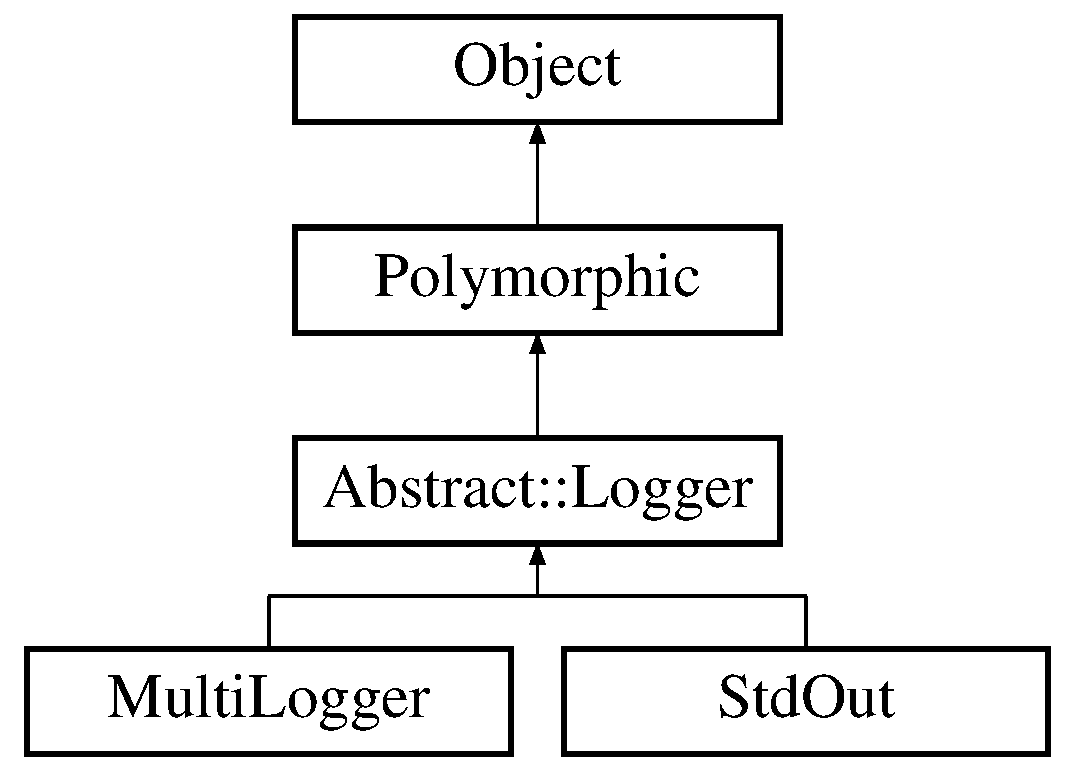
\includegraphics[height=4.000000cm]{classAbstract_1_1Logger}
\end{center}
\end{figure}
\subsection*{Public Member Functions}
\begin{DoxyCompactItemize}
\item 
\hypertarget{classAbstract_1_1Logger_a9fa51f5e2c0d0965e04c4944012f8165}{}\label{classAbstract_1_1Logger_a9fa51f5e2c0d0965e04c4944012f8165} 
virtual void {\bfseries write} (const std\+::string \&s)=0
\item 
\hypertarget{classAbstract_1_1Logger_a459302696cbf474bf713661afac38e4d}{}\label{classAbstract_1_1Logger_a459302696cbf474bf713661afac38e4d} 
\hyperlink{classAbstract_1_1Logger}{Logger} \& {\bfseries operator$<$$<$} (const std\+::string \&s)
\end{DoxyCompactItemize}


The documentation for this class was generated from the following file\+:\begin{DoxyCompactItemize}
\item 
/home/pavel/projects/astro/sph2/src/system/logger.\+h\end{DoxyCompactItemize}

\hypertarget{classLutKernel}{}\section{Lut\+Kernel Class Reference}
\label{classLutKernel}\index{Lut\+Kernel@{Lut\+Kernel}}


A look-\/up table approximation of the kernel. Can be constructed from any S\+PH kernel.  




{\ttfamily \#include $<$kernel.\+h$>$}

Inheritance diagram for Lut\+Kernel\+:\begin{figure}[H]
\begin{center}
\leavevmode
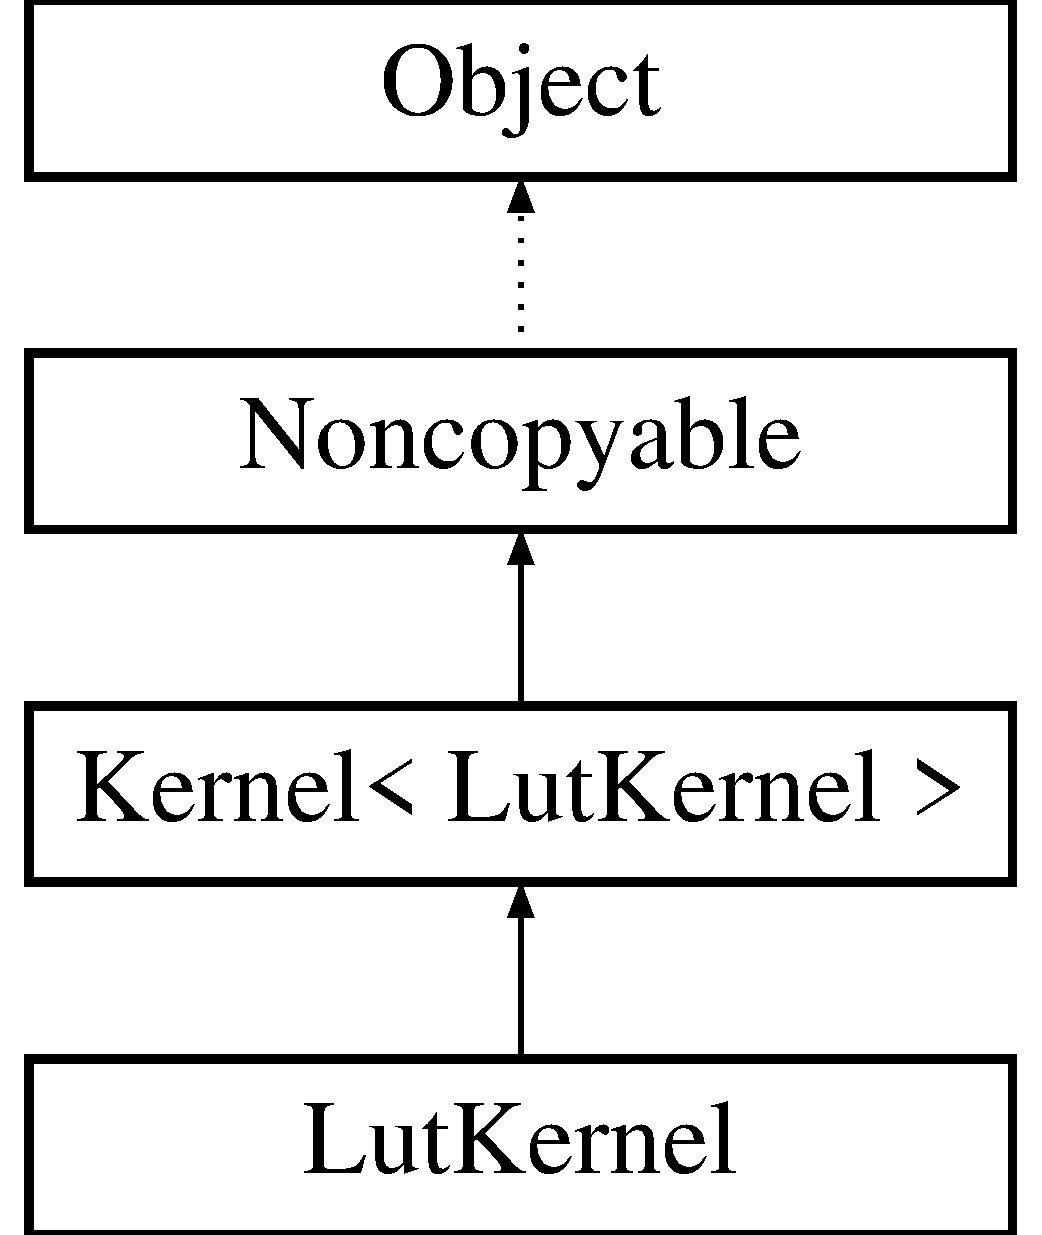
\includegraphics[height=4.000000cm]{classLutKernel}
\end{center}
\end{figure}
\subsection*{Public Member Functions}
\begin{DoxyCompactItemize}
\item 
{\footnotesize template$<$typename T\+Kernel $>$ }\\\hyperlink{classLutKernel_a91a4f8b38a4b859536bcfda2140d1585}{Lut\+Kernel} (T\+Kernel \&\&source)
\item 
\hypertarget{classLutKernel_a42e116366354b4e7d919bb648dc6cd63}{}\label{classLutKernel_a42e116366354b4e7d919bb648dc6cd63} 
\hyperlink{classLutKernel}{Lut\+Kernel} \& {\bfseries operator=} (\hyperlink{classLutKernel}{Lut\+Kernel} \&\&other)
\item 
\hypertarget{classLutKernel_aa6a3fac1190441a9f598e6a8a7793e8a}{}\label{classLutKernel_aa6a3fac1190441a9f598e6a8a7793e8a} 
I\+N\+L\+I\+NE bool {\bfseries is\+Init} () const
\item 
\hypertarget{classLutKernel_af7ee74fa4adeef6771d176f046ac8ba0}{}\label{classLutKernel_af7ee74fa4adeef6771d176f046ac8ba0} 
I\+N\+L\+I\+NE Float {\bfseries radius} () const
\item 
\hypertarget{classLutKernel_a22469f5512062c4c06814f804aafa2d0}{}\label{classLutKernel_a22469f5512062c4c06814f804aafa2d0} 
I\+N\+L\+I\+NE Float {\bfseries value\+Impl} (const Float \&q\+Sqr) const
\item 
\hypertarget{classLutKernel_a60aeff7bf864f9f856ebb1872f5316e8}{}\label{classLutKernel_a60aeff7bf864f9f856ebb1872f5316e8} 
I\+N\+L\+I\+NE Float {\bfseries grad\+Impl} (const Float \&q\+Sqr) const
\end{DoxyCompactItemize}


\subsection{Detailed Description}
A look-\/up table approximation of the kernel. Can be constructed from any S\+PH kernel. 

\subsection{Constructor \& Destructor Documentation}
\hypertarget{classLutKernel_a91a4f8b38a4b859536bcfda2140d1585}{}\label{classLutKernel_a91a4f8b38a4b859536bcfda2140d1585} 
\index{Lut\+Kernel@{Lut\+Kernel}!Lut\+Kernel@{Lut\+Kernel}}
\index{Lut\+Kernel@{Lut\+Kernel}!Lut\+Kernel@{Lut\+Kernel}}
\subsubsection{\texorpdfstring{Lut\+Kernel()}{LutKernel()}}
{\footnotesize\ttfamily template$<$typename T\+Kernel $>$ \\
Lut\+Kernel\+::\+Lut\+Kernel (\begin{DoxyParamCaption}\item[{T\+Kernel \&\&}]{source }\end{DoxyParamCaption})\hspace{0.3cm}{\ttfamily [inline]}}

\begin{DoxyRefDesc}{Todo}
\item[\hyperlink{todo__todo000017}{Todo}]re-\/normalize? \end{DoxyRefDesc}


The documentation for this class was generated from the following file\+:\begin{DoxyCompactItemize}
\item 
/home/pavel/projects/astro/sph2/src/kernel/kernel.\+h\end{DoxyCompactItemize}

\hypertarget{classMatrix}{}\section{Matrix Class Reference}
\label{classMatrix}\index{Matrix@{Matrix}}
Inheritance diagram for Matrix\+:\begin{figure}[H]
\begin{center}
\leavevmode
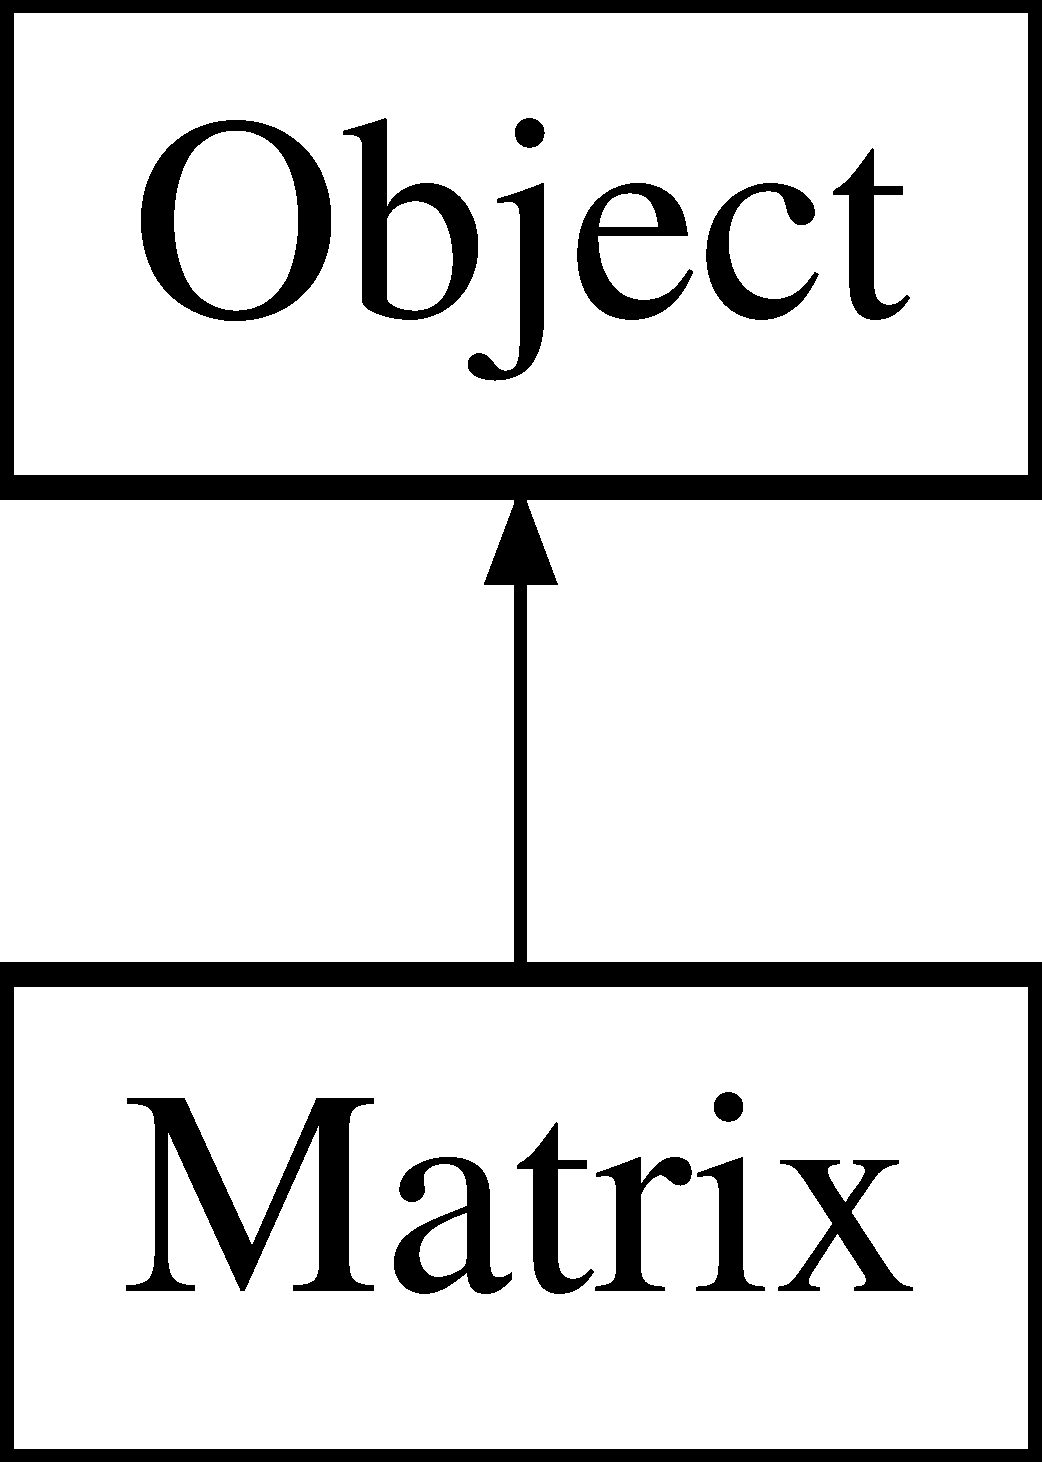
\includegraphics[height=2.000000cm]{classMatrix}
\end{center}
\end{figure}
\subsection*{Public Member Functions}
\begin{DoxyCompactItemize}
\item 
\hypertarget{classMatrix_abcf708e864ed3d9db2c3b317c5e529ab}{}\label{classMatrix_abcf708e864ed3d9db2c3b317c5e529ab} 
{\bfseries Matrix} (const \hyperlink{classMatrix}{Matrix} \&other)
\item 
\hypertarget{classMatrix_aa8221a09ab250cb0c6cf65c53d43b780}{}\label{classMatrix_aa8221a09ab250cb0c6cf65c53d43b780} 
{\bfseries Matrix} (\hyperlink{classMatrix}{Matrix} \&\&other)
\item 
\hypertarget{classMatrix_a95c1e29ca70d8cadbcf55c6a86fbf837}{}\label{classMatrix_a95c1e29ca70d8cadbcf55c6a86fbf837} 
{\bfseries Matrix} (const \hyperlink{classBasicVector}{Vector} \&v1, const \hyperlink{classBasicVector}{Vector} \&v2, const \hyperlink{classBasicVector}{Vector} \&v3)
\item 
\hypertarget{classMatrix_a935f841ddb4536f45a5ec161ccec0d15}{}\label{classMatrix_a935f841ddb4536f45a5ec161ccec0d15} 
const double $\ast$ {\bfseries operator\mbox{[}$\,$\mbox{]}} (uint1 idx) const
\item 
\hypertarget{classMatrix_af5369ef5c65853353090112a676320c2}{}\label{classMatrix_af5369ef5c65853353090112a676320c2} 
double $\ast$ {\bfseries operator\mbox{[}$\,$\mbox{]}} (uint1 idx)
\item 
\hypertarget{classMatrix_ad0c96cdea0d2ae3403653ca90aa70796}{}\label{classMatrix_ad0c96cdea0d2ae3403653ca90aa70796} 
\hyperlink{classMatrix}{Matrix} {\bfseries Transpose} () const
\item 
\hypertarget{classMatrix_ad5f101877c4a10988bf7f128a9c248d8}{}\label{classMatrix_ad5f101877c4a10988bf7f128a9c248d8} 
\hyperlink{classMatrix}{Matrix} {\bfseries Inverse} () const
\item 
\hypertarget{classMatrix_aa64659e33d639e69716034b2091bdaf6}{}\label{classMatrix_aa64659e33d639e69716034b2091bdaf6} 
\hyperlink{classMatrix}{Matrix} {\bfseries Remove\+Translation} () const
\item 
\hypertarget{classMatrix_a05874398dc7839c74fb090c6bfe17e0a}{}\label{classMatrix_a05874398dc7839c74fb090c6bfe17e0a} 
void {\bfseries To\+Log} (T\+Log $\ast$log=\&S\+T\+D\+\_\+\+O\+UT) const
\end{DoxyCompactItemize}
\subsection*{Static Public Member Functions}
\begin{DoxyCompactItemize}
\item 
\hypertarget{classMatrix_a71946b221577fae7a86177bca76d9d96}{}\label{classMatrix_a71946b221577fae7a86177bca76d9d96} 
static \hyperlink{classMatrix}{Matrix} {\bfseries Identity} ()
\item 
\hypertarget{classMatrix_aee442afe6336844ea24a0a9d1c4a70b4}{}\label{classMatrix_aee442afe6336844ea24a0a9d1c4a70b4} 
static \hyperlink{classMatrix}{Matrix} {\bfseries Null} ()
\item 
\hypertarget{classMatrix_ae92199d7a89aad1f3f501a75ed668392}{}\label{classMatrix_ae92199d7a89aad1f3f501a75ed668392} 
static \hyperlink{classMatrix}{Matrix} {\bfseries RotateX} (double a)
\item 
\hypertarget{classMatrix_a6c1deaa568066a0a058c2120701ca661}{}\label{classMatrix_a6c1deaa568066a0a058c2120701ca661} 
static \hyperlink{classMatrix}{Matrix} {\bfseries RotateY} (double a)
\item 
\hypertarget{classMatrix_ab7d522fde5f8c5060898456aa1caf496}{}\label{classMatrix_ab7d522fde5f8c5060898456aa1caf496} 
static \hyperlink{classMatrix}{Matrix} {\bfseries RotateZ} (double a)
\item 
\hypertarget{classMatrix_a28fcbc2c17a3f1192c1d057dce01f8a6}{}\label{classMatrix_a28fcbc2c17a3f1192c1d057dce01f8a6} 
static \hyperlink{classMatrix}{Matrix} {\bfseries Rotate\+Euler} (double a, double b, double c)
\item 
\hypertarget{classMatrix_ac04a830d4b99b478088812ba0ee3cd57}{}\label{classMatrix_ac04a830d4b99b478088812ba0ee3cd57} 
static \hyperlink{classMatrix}{Matrix} {\bfseries Rotate\+Axis} (const T\+Vector \&axis, double a)
\item 
\hypertarget{classMatrix_a6d94a46039304c204ff501a3cbd94892}{}\label{classMatrix_a6d94a46039304c204ff501a3cbd94892} 
static \hyperlink{classMatrix}{Matrix} {\bfseries Translate} (const T\+Vector \&t)
\item 
\hypertarget{classMatrix_a9e247a9f062fb569f497aaf5615a8da0}{}\label{classMatrix_a9e247a9f062fb569f497aaf5615a8da0} 
static \hyperlink{classMatrix}{Matrix} {\bfseries Scale} (double x, double y, double z)
\item 
\hypertarget{classMatrix_aee12e50e8a87b6bcdc0acdfc8ad42695}{}\label{classMatrix_aee12e50e8a87b6bcdc0acdfc8ad42695} 
static \hyperlink{classMatrix}{Matrix} {\bfseries Scale} (double s)
\item 
\hypertarget{classMatrix_a2f65f62ed9ebe96aa92ef9ce45045e6e}{}\label{classMatrix_a2f65f62ed9ebe96aa92ef9ce45045e6e} 
static \hyperlink{classMatrix}{Matrix} {\bfseries T\+RS} (const T\+Vector \&t, const T\+Vector \&r, const T\+Vector \&s)
\end{DoxyCompactItemize}


The documentation for this class was generated from the following file\+:\begin{DoxyCompactItemize}
\item 
/home/pavel/projects/astro/sph2/src/geometry/tensor.\+h\end{DoxyCompactItemize}

\hypertarget{structSph_1_1metric__L1}{}\section{Sph\+:\+:metric\+\_\+\+L1 Struct Reference}
\label{structSph_1_1metric__L1}\index{Sph\+::metric\+\_\+\+L1@{Sph\+::metric\+\_\+\+L1}}


{\ttfamily \#include $<$nanoflann.\+h$>$}

\subsection*{Classes}
\begin{DoxyCompactItemize}
\item 
struct \hyperlink{structSph_1_1metric__L1_1_1traits}{traits}
\end{DoxyCompactItemize}


\subsection{Detailed Description}
Metaprogramming helper traits class for the L1 (Manhattan) metric 

The documentation for this struct was generated from the following file\+:\begin{DoxyCompactItemize}
\item 
/home/pavel/projects/astro/sph2/src/tree/nanoflann.\+h\end{DoxyCompactItemize}

\hypertarget{structSph_1_1metric__L2}{}\section{Sph\+:\+:metric\+\_\+\+L2 Struct Reference}
\label{structSph_1_1metric__L2}\index{Sph\+::metric\+\_\+\+L2@{Sph\+::metric\+\_\+\+L2}}


{\ttfamily \#include $<$nanoflann.\+h$>$}

\subsection*{Classes}
\begin{DoxyCompactItemize}
\item 
struct \hyperlink{structSph_1_1metric__L2_1_1traits}{traits}
\end{DoxyCompactItemize}


\subsection{Detailed Description}
Metaprogramming helper traits class for the L2 (Euclidean) metric 

The documentation for this struct was generated from the following file\+:\begin{DoxyCompactItemize}
\item 
/home/pavel/projects/astro/sph2/src/tree/nanoflann.\+h\end{DoxyCompactItemize}

\hypertarget{structSph_1_1metric__L2__Simple}{}\section{Sph\+:\+:metric\+\_\+\+L2\+\_\+\+Simple Struct Reference}
\label{structSph_1_1metric__L2__Simple}\index{Sph\+::metric\+\_\+\+L2\+\_\+\+Simple@{Sph\+::metric\+\_\+\+L2\+\_\+\+Simple}}


{\ttfamily \#include $<$nanoflann.\+h$>$}

\subsection*{Classes}
\begin{DoxyCompactItemize}
\item 
struct \hyperlink{structSph_1_1metric__L2__Simple_1_1traits}{traits}
\end{DoxyCompactItemize}


\subsection{Detailed Description}
Metaprogramming helper traits class for the L2\+\_\+simple (Euclidean) metric 

The documentation for this struct was generated from the following file\+:\begin{DoxyCompactItemize}
\item 
/home/pavel/projects/astro/sph2/src/tree/nanoflann.\+h\end{DoxyCompactItemize}

\hypertarget{classMultiLogger}{}\section{Multi\+Logger Class Reference}
\label{classMultiLogger}\index{Multi\+Logger@{Multi\+Logger}}


Class holding multiple loggers and writing messages to all of them. The objects is the owner of loggers.  




{\ttfamily \#include $<$logger.\+h$>$}

Inheritance diagram for Multi\+Logger\+:\begin{figure}[H]
\begin{center}
\leavevmode
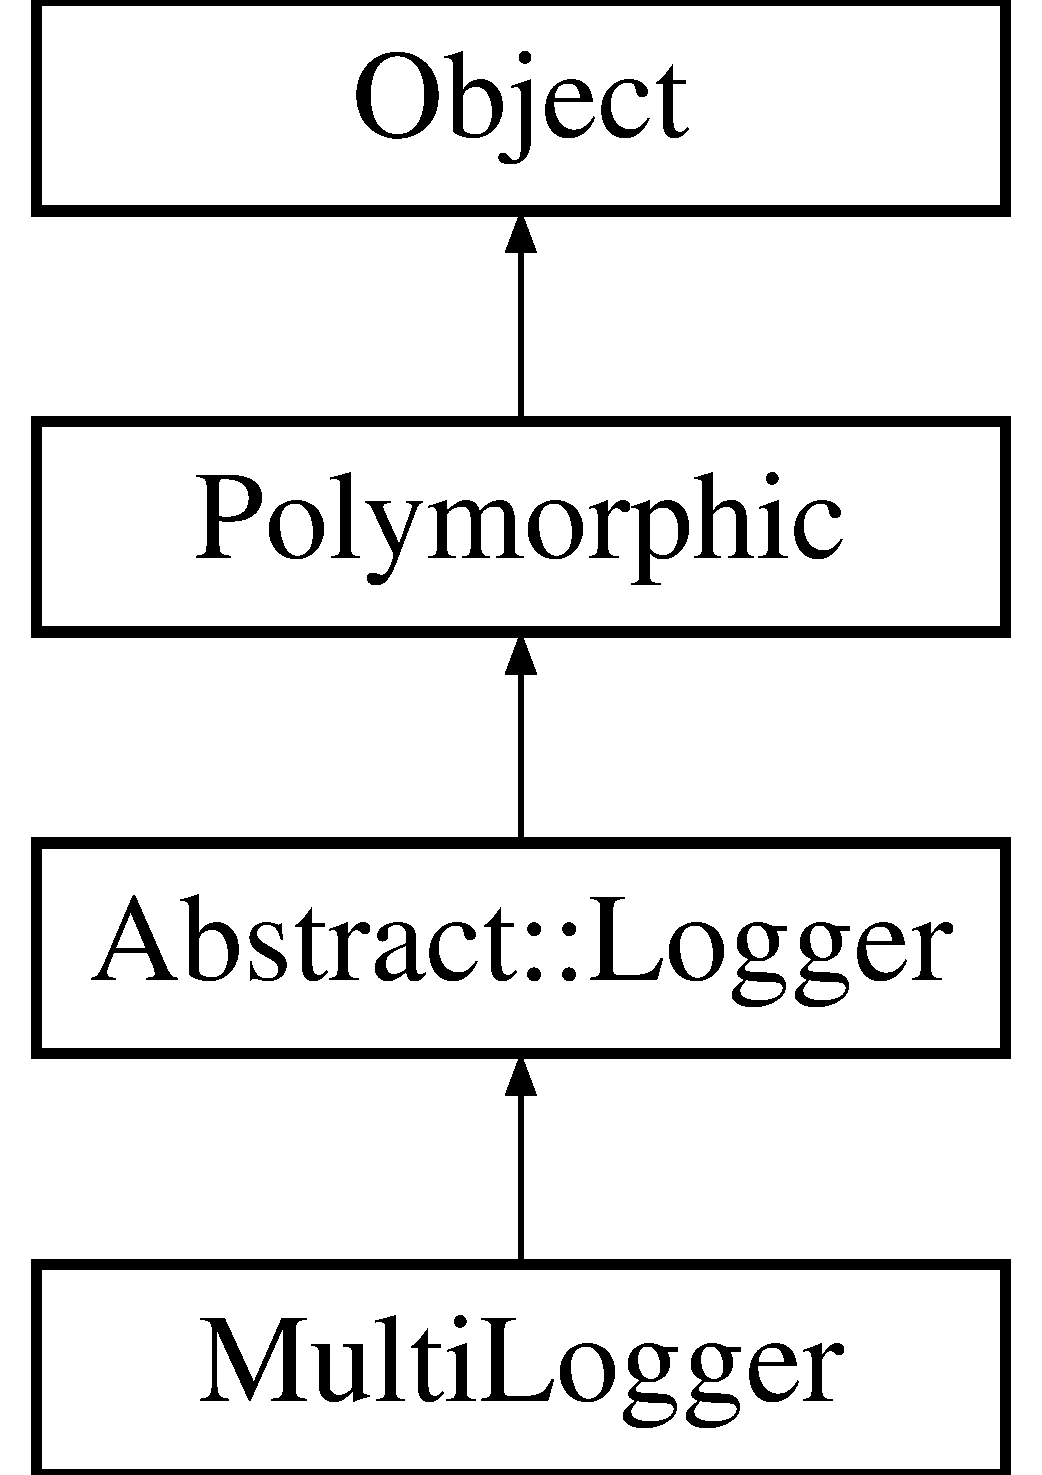
\includegraphics[height=4.000000cm]{classMultiLogger}
\end{center}
\end{figure}
\subsection*{Public Member Functions}
\begin{DoxyCompactItemize}
\item 
\hypertarget{classMultiLogger_a96e4c7e567d5777c2e5c5234f6475ff6}{}\label{classMultiLogger_a96e4c7e567d5777c2e5c5234f6475ff6} 
int {\bfseries get\+Logger\+Cnt} () const
\item 
\hypertarget{classMultiLogger_a3f0254d865a24ba628f95567bb52da73}{}\label{classMultiLogger_a3f0254d865a24ba628f95567bb52da73} 
void {\bfseries add} (\hyperlink{classAbstract_1_1Logger}{Abstract\+::\+Logger} $\ast$logger)
\item 
\hypertarget{classMultiLogger_a1926134f872f630aa5825dfc84888d0c}{}\label{classMultiLogger_a1926134f872f630aa5825dfc84888d0c} 
virtual void {\bfseries write} (const std\+::string \&s) override
\end{DoxyCompactItemize}


\subsection{Detailed Description}
Class holding multiple loggers and writing messages to all of them. The objects is the owner of loggers. 

The documentation for this class was generated from the following file\+:\begin{DoxyCompactItemize}
\item 
/home/pavel/projects/astro/sph2/src/system/logger.\+h\end{DoxyCompactItemize}

\hypertarget{structNeighbourRecord}{}\section{Neighbour\+Record Struct Reference}
\label{structNeighbourRecord}\index{Neighbour\+Record@{Neighbour\+Record}}
\subsection*{Public Attributes}
\begin{DoxyCompactItemize}
\item 
\hypertarget{structNeighbourRecord_a156deb791fa1777f25497c491add4deb}{}\label{structNeighbourRecord_a156deb791fa1777f25497c491add4deb} 
int {\bfseries index}
\item 
\hypertarget{structNeighbourRecord_a95b76094dd1b5f9c2a76fcbf7cc55d83}{}\label{structNeighbourRecord_a95b76094dd1b5f9c2a76fcbf7cc55d83} 
Float {\bfseries distance\+Sqr}
\end{DoxyCompactItemize}


The documentation for this struct was generated from the following file\+:\begin{DoxyCompactItemize}
\item 
/home/pavel/projects/astro/sph2/src/tree/finder.\+h\end{DoxyCompactItemize}

\hypertarget{structNestedType}{}\section{Nested\+Type$<$ T $>$ Struct Template Reference}
\label{structNestedType}\index{Nested\+Type$<$ T $>$@{Nested\+Type$<$ T $>$}}


Type traits.  




{\ttfamily \#include $<$traits.\+h$>$}

\subsection*{Public Types}
\begin{DoxyCompactItemize}
\item 
\hypertarget{structNestedType_a4275ea73323189a35f65e74feca39f05}{}\label{structNestedType_a4275ea73323189a35f65e74feca39f05} 
using {\bfseries Type} = T
\end{DoxyCompactItemize}


\subsection{Detailed Description}
\subsubsection*{template$<$typename T$>$\newline
struct Nested\+Type$<$ T $>$}

Type traits. 

The documentation for this struct was generated from the following file\+:\begin{DoxyCompactItemize}
\item 
/home/pavel/projects/astro/sph2/src/core/traits.\+h\end{DoxyCompactItemize}

\hypertarget{structNestedType_3_01TStorage_3_01T_01_4_01_4}{}\section{Nested\+Type$<$ T\+Storage$<$ T $>$ $>$ Struct Template Reference}
\label{structNestedType_3_01TStorage_3_01T_01_4_01_4}\index{Nested\+Type$<$ T\+Storage$<$ T $>$ $>$@{Nested\+Type$<$ T\+Storage$<$ T $>$ $>$}}
\subsection*{Public Types}
\begin{DoxyCompactItemize}
\item 
\hypertarget{structNestedType_3_01TStorage_3_01T_01_4_01_4_a0e61555b2e9dffebf6c1bbcb728e225d}{}\label{structNestedType_3_01TStorage_3_01T_01_4_01_4_a0e61555b2e9dffebf6c1bbcb728e225d} 
using {\bfseries Type} = typename \hyperlink{structNestedType}{Nested\+Type}$<$ T $>$\+::Type
\end{DoxyCompactItemize}


The documentation for this struct was generated from the following file\+:\begin{DoxyCompactItemize}
\item 
/home/pavel/projects/astro/sph2/src/core/traits.\+h\end{DoxyCompactItemize}

\hypertarget{structSph_1_1KDTreeSingleIndexAdaptor_1_1Node}{}\section{Sph\+:\+:K\+D\+Tree\+Single\+Index\+Adaptor$<$ Distance, Dataset\+Adaptor, D\+IM, Index\+Type $>$\+:\+:Node Struct Reference}
\label{structSph_1_1KDTreeSingleIndexAdaptor_1_1Node}\index{Sph\+::\+K\+D\+Tree\+Single\+Index\+Adaptor$<$ Distance, Dataset\+Adaptor, D\+I\+M, Index\+Type $>$\+::\+Node@{Sph\+::\+K\+D\+Tree\+Single\+Index\+Adaptor$<$ Distance, Dataset\+Adaptor, D\+I\+M, Index\+Type $>$\+::\+Node}}
\subsection*{Public Attributes}
\begin{DoxyCompactItemize}
\item 
\begin{tabbing}
xx\=xx\=xx\=xx\=xx\=xx\=xx\=xx\=xx\=\kill
union \{\\
\>struct {\bfseries leaf} \{\\
\>\>IndexType {\bfseries left}\\
\>\>IndexType \hyperlink{structSph_1_1KDTreeSingleIndexAdaptor_1_1Node_af113c9c56164fcb7f8162442c2dce67a}{right}\\
\>\>\>{\em Indices of points in leaf node. }\\
\>\} {\bfseries lr}\\
\>struct {\bfseries nonleaf} \{\\
\>\>int \hyperlink{structSph_1_1KDTreeSingleIndexAdaptor_1_1Node_a613c1685d60dec4d84508a6a84455172}{divfeat}\\
\>\>\>{\em Dimension used for subdivision. }\\
\>\>DistanceType {\bfseries divlow}\\
\>\>DistanceType \hyperlink{structSph_1_1KDTreeSingleIndexAdaptor_1_1Node_afb61f548f4bcde7e99228f7820566e2b}{divhigh}\\
\>\>\>{\em The values used for subdivision. }\\
\>\} {\bfseries sub}\\
\} \hyperlink{structSph_1_1KDTreeSingleIndexAdaptor_1_1Node_a5b93ce4ef4b68d3222e41fcf4802d337}{node\_type}\\

\end{tabbing}\item 
\hypertarget{structSph_1_1KDTreeSingleIndexAdaptor_1_1Node_a744802d3870a701d8c688be4dcb19730}{}\label{structSph_1_1KDTreeSingleIndexAdaptor_1_1Node_a744802d3870a701d8c688be4dcb19730} 
\hyperlink{structSph_1_1KDTreeSingleIndexAdaptor_1_1Node}{Node} $\ast$ {\bfseries child1}
\item 
\hypertarget{structSph_1_1KDTreeSingleIndexAdaptor_1_1Node_a52db4680e40cb1d554380c60913bfc05}{}\label{structSph_1_1KDTreeSingleIndexAdaptor_1_1Node_a52db4680e40cb1d554380c60913bfc05} 
\hyperlink{structSph_1_1KDTreeSingleIndexAdaptor_1_1Node}{Node} $\ast$ \hyperlink{structSph_1_1KDTreeSingleIndexAdaptor_1_1Node_a52db4680e40cb1d554380c60913bfc05}{child2}
\begin{DoxyCompactList}\small\item\em Child nodes (both=N\+U\+LL mean its a leaf node) \end{DoxyCompactList}\end{DoxyCompactItemize}


\subsection{Member Data Documentation}
\hypertarget{structSph_1_1KDTreeSingleIndexAdaptor_1_1Node_a5b93ce4ef4b68d3222e41fcf4802d337}{}\label{structSph_1_1KDTreeSingleIndexAdaptor_1_1Node_a5b93ce4ef4b68d3222e41fcf4802d337} 
\index{Sph\+::\+K\+D\+Tree\+Single\+Index\+Adaptor\+::\+Node@{Sph\+::\+K\+D\+Tree\+Single\+Index\+Adaptor\+::\+Node}!node\+\_\+type@{node\+\_\+type}}
\index{node\+\_\+type@{node\+\_\+type}!Sph\+::\+K\+D\+Tree\+Single\+Index\+Adaptor\+::\+Node@{Sph\+::\+K\+D\+Tree\+Single\+Index\+Adaptor\+::\+Node}}
\subsubsection{\texorpdfstring{node\+\_\+type}{node\_type}}
{\footnotesize\ttfamily union \{ ... \}   \hyperlink{classSph_1_1KDTreeSingleIndexAdaptor}{Sph\+::\+K\+D\+Tree\+Single\+Index\+Adaptor}$<$ Distance, Dataset\+Adaptor, D\+IM, Index\+Type $>$\+::Node\+::node\+\_\+type}

\hyperlink{classUnion}{Union} used because a node can be either a L\+E\+AF node or a non-\/leaf node, so both data fields are never used simultaneously 

The documentation for this struct was generated from the following file\+:\begin{DoxyCompactItemize}
\item 
/home/pavel/projects/astro/sph2/src/tree/nanoflann.\+h\end{DoxyCompactItemize}

\hypertarget{structNode}{}\section{Node$<$ T, d $>$ Struct Template Reference}
\label{structNode}\index{Node$<$ T, d $>$@{Node$<$ T, d $>$}}
\subsection*{Public Attributes}
\begin{DoxyCompactItemize}
\item 
\hypertarget{structNode_ac1cae505fa4c2d59779ce2fe9fd61b5d}{}\label{structNode_ac1cae505fa4c2d59779ce2fe9fd61b5d} 
T $\ast$ {\bfseries data}
\item 
\hypertarget{structNode_afe25e038145930b4b579cec9331f140f}{}\label{structNode_afe25e038145930b4b579cec9331f140f} 
\hyperlink{structNode}{Node} $\ast$ {\bfseries children} \mbox{[}1$<$$<$ d\mbox{]}
\end{DoxyCompactItemize}


The documentation for this struct was generated from the following file\+:\begin{DoxyCompactItemize}
\item 
/home/pavel/projects/astro/sph2/src/tree/octree.\+h\end{DoxyCompactItemize}

\hypertarget{classNoncopyable}{}\section{Noncopyable Class Reference}
\label{classNoncopyable}\index{Noncopyable@{Noncopyable}}


\hyperlink{classObject}{Object} with deleted copy constructor and copy operator.  




{\ttfamily \#include $<$object.\+h$>$}

Inheritance diagram for Noncopyable\+:\begin{figure}[H]
\begin{center}
\leavevmode
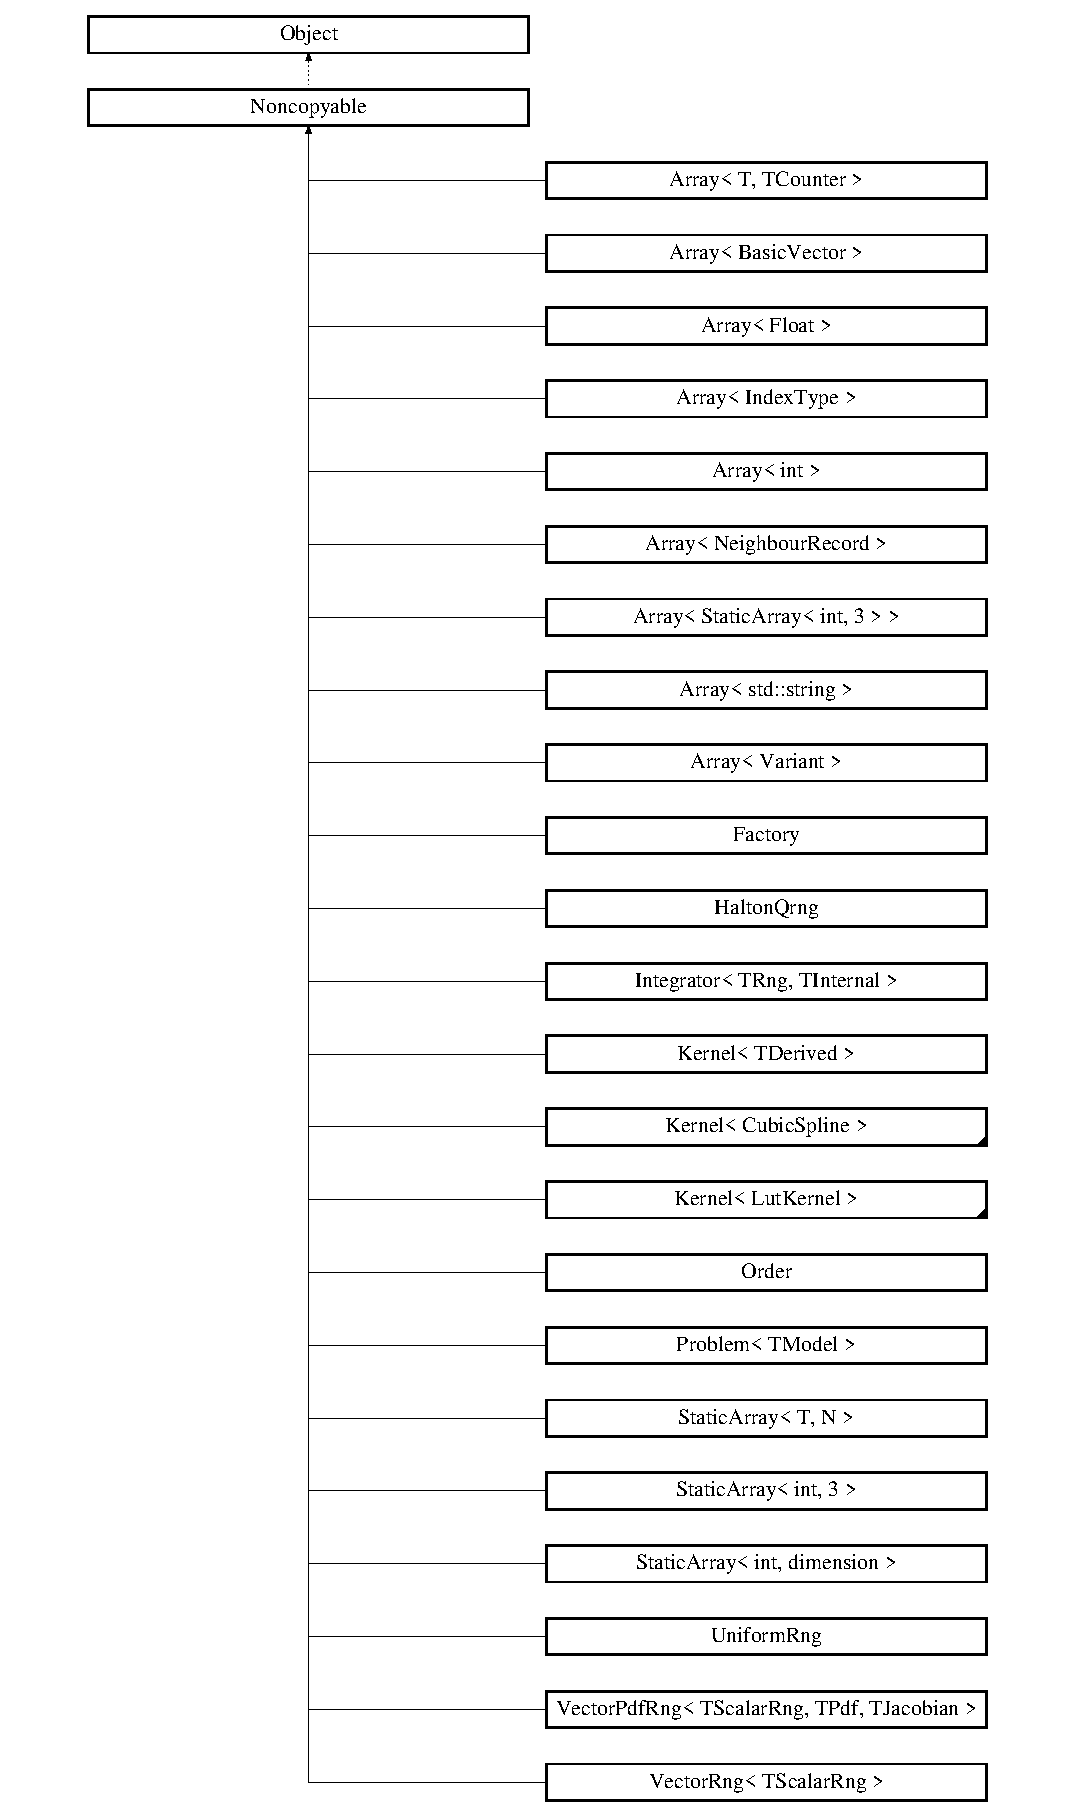
\includegraphics[height=12.000000cm]{classNoncopyable}
\end{center}
\end{figure}
\subsection*{Public Member Functions}
\begin{DoxyCompactItemize}
\item 
\hypertarget{classNoncopyable_a2ef4eb7cdf95677b046151206e10696b}{}\label{classNoncopyable_a2ef4eb7cdf95677b046151206e10696b} 
{\bfseries Noncopyable} (const \hyperlink{classNoncopyable}{Noncopyable} \&)=delete
\item 
\hypertarget{classNoncopyable_a09a0a26fe338b78dd3385142f07d5a25}{}\label{classNoncopyable_a09a0a26fe338b78dd3385142f07d5a25} 
\hyperlink{classNoncopyable}{Noncopyable} \& {\bfseries operator=} (const \hyperlink{classNoncopyable}{Noncopyable} \&)=delete
\end{DoxyCompactItemize}


\subsection{Detailed Description}
\hyperlink{classObject}{Object} with deleted copy constructor and copy operator. 

The documentation for this class was generated from the following file\+:\begin{DoxyCompactItemize}
\item 
/home/pavel/projects/astro/sph2/src/core/object.\+h\end{DoxyCompactItemize}

\hypertarget{structNothingType}{}\section{Nothing\+Type Struct Reference}
\label{structNothingType}\index{Nothing\+Type@{Nothing\+Type}}


The documentation for this struct was generated from the following file\+:\begin{DoxyCompactItemize}
\item 
/home/pavel/projects/astro/sph2/src/structs/optional.\+h\end{DoxyCompactItemize}

\hypertarget{classObject}{}\section{Object Class Reference}
\label{classObject}\index{Object@{Object}}


Basic object from which all types are derived.  




{\ttfamily \#include $<$object.\+h$>$}

Inheritance diagram for Object\+:\begin{figure}[H]
\begin{center}
\leavevmode
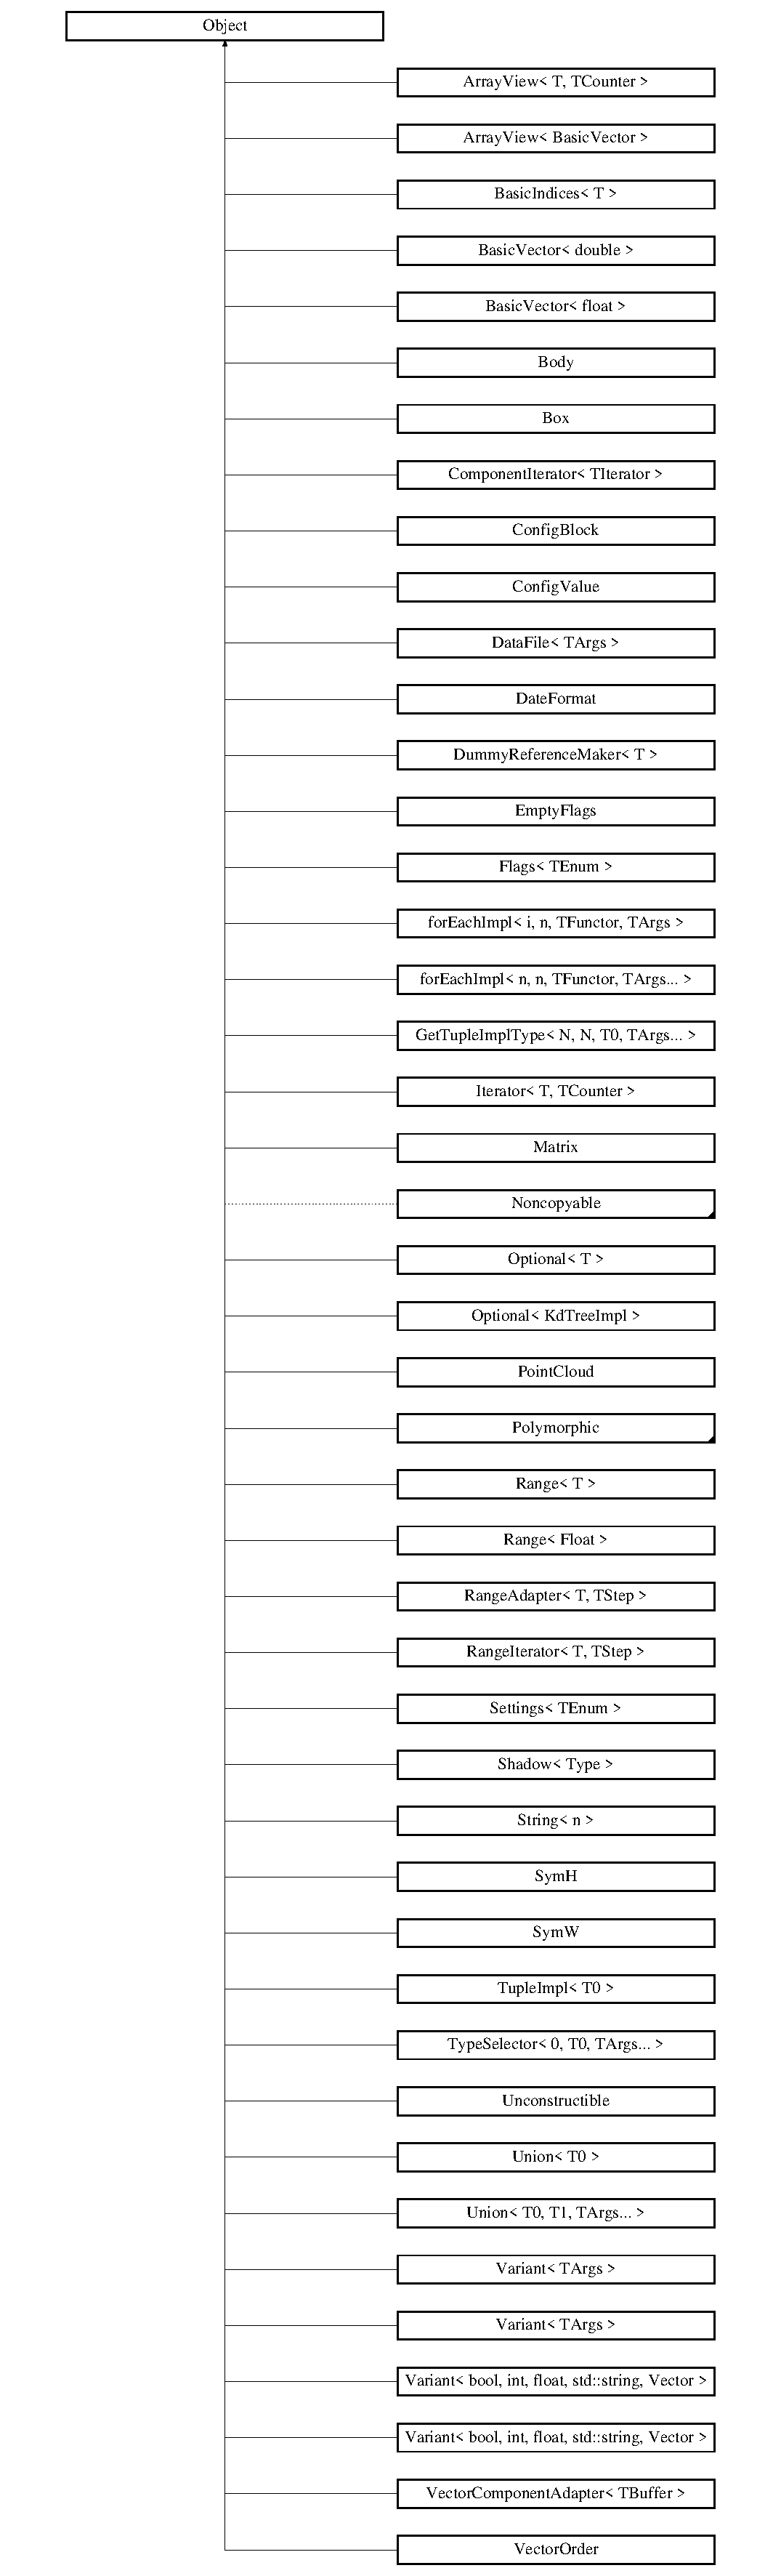
\includegraphics[height=12.000000cm]{classObject}
\end{center}
\end{figure}


\subsection{Detailed Description}
Basic object from which all types are derived. 

The documentation for this class was generated from the following file\+:\begin{DoxyCompactItemize}
\item 
/home/pavel/projects/astro/sph2/src/core/object.\+h\end{DoxyCompactItemize}

\hypertarget{classOctree}{}\section{Octree$<$ T, d $>$ Class Template Reference}
\label{classOctree}\index{Octree$<$ T, d $>$@{Octree$<$ T, d $>$}}
\subsection*{Public Member Functions}
\begin{DoxyCompactItemize}
\item 
\hypertarget{classOctree_a1222d95695ff4a23997b1898849f156b}{}\label{classOctree_a1222d95695ff4a23997b1898849f156b} 
{\bfseries Octree} (const \hyperlink{classArray}{Array}$<$ \hyperlink{classBasicVector}{Vector}$<$ T, d $>$$>$ \&vecs)
\end{DoxyCompactItemize}


The documentation for this class was generated from the following file\+:\begin{DoxyCompactItemize}
\item 
/home/pavel/projects/astro/sph2/src/tree/octree.\+h\end{DoxyCompactItemize}

\hypertarget{classOptional}{}\section{Optional$<$ T $>$ Class Template Reference}
\label{classOptional}\index{Optional$<$ T $>$@{Optional$<$ T $>$}}


{\ttfamily \#include $<$optional.\+h$>$}

Inheritance diagram for Optional$<$ T $>$\+:\begin{figure}[H]
\begin{center}
\leavevmode
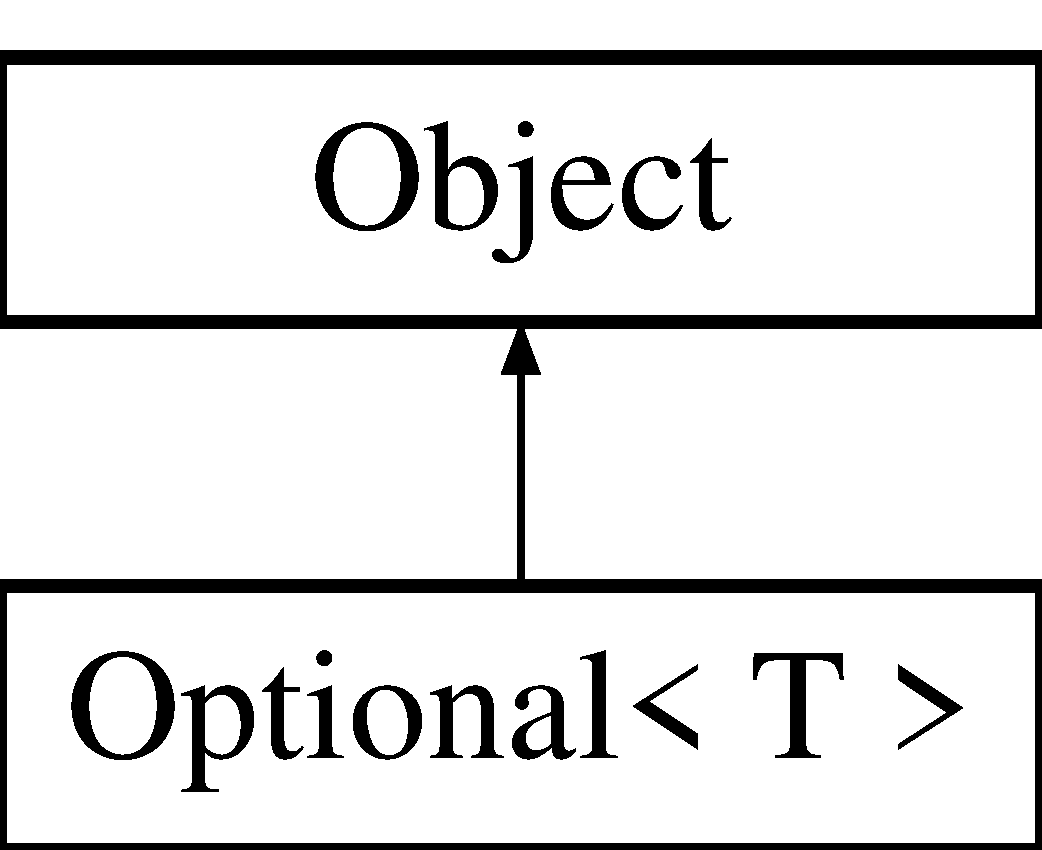
\includegraphics[height=2.000000cm]{classOptional}
\end{center}
\end{figure}
\subsection*{Public Member Functions}
\begin{DoxyCompactItemize}
\item 
\hypertarget{classOptional_af4deb96207fa2285779bbb8c073acbcd}{}\label{classOptional_af4deb96207fa2285779bbb8c073acbcd} 
\hyperlink{classOptional_af4deb96207fa2285779bbb8c073acbcd}{Optional} (const Raw\+Type \&t)
\begin{DoxyCompactList}\small\item\em Copy constuctor from stored value. Initialize the optional value. \end{DoxyCompactList}\item 
\hypertarget{classOptional_a450e6403178db88f2fd9ec3a1391d858}{}\label{classOptional_a450e6403178db88f2fd9ec3a1391d858} 
\hyperlink{classOptional_a450e6403178db88f2fd9ec3a1391d858}{Optional} (Raw\+Type \&\&t)
\begin{DoxyCompactList}\small\item\em Move constuctor from stored value. Initialize the optional value. \end{DoxyCompactList}\item 
\hyperlink{classOptional_a099b0dce0d5fedf466ca51057dd9eb5c}{Optional} (const \hyperlink{classOptional}{Optional} \&other)
\item 
\hyperlink{classOptional_a114c41318cb918540e6b0bac8159239c}{Optional} (\hyperlink{classOptional}{Optional} \&\&other)
\item 
\hypertarget{classOptional_af86726f19377893d4a73e2d05c8ca513}{}\label{classOptional_af86726f19377893d4a73e2d05c8ca513} 
\hyperlink{classOptional_af86726f19377893d4a73e2d05c8ca513}{Optional} (const \hyperlink{structNothingType}{Nothing\+Type} \&)
\begin{DoxyCompactList}\small\item\em Construct uninitialized. \end{DoxyCompactList}\item 
\hypertarget{classOptional_a45557bde636d60b1a7c3a089b4e579bb}{}\label{classOptional_a45557bde636d60b1a7c3a089b4e579bb} 
\hyperlink{classOptional_a45557bde636d60b1a7c3a089b4e579bb}{$\sim$\+Optional} ()
\begin{DoxyCompactList}\small\item\em Destructor. \end{DoxyCompactList}\item 
{\footnotesize template$<$typename... T\+Args$>$ }\\void \hyperlink{classOptional_a2e0236b5bd0e4877d7db446cf0bb784e}{emplace} (T\+Args \&\&... args)
\item 
\hypertarget{classOptional_a5a8c6588ed666899bd852579e4580141}{}\label{classOptional_a5a8c6588ed666899bd852579e4580141} 
\hyperlink{classOptional}{Optional} \& \hyperlink{classOptional_a5a8c6588ed666899bd852579e4580141}{operator=} (const Raw\+Type \&t)
\begin{DoxyCompactList}\small\item\em Copy operator. \end{DoxyCompactList}\item 
\hypertarget{classOptional_a622aae8c71487f2e49fa5c47e6d34baa}{}\label{classOptional_a622aae8c71487f2e49fa5c47e6d34baa} 
\hyperlink{classOptional}{Optional} \& \hyperlink{classOptional_a622aae8c71487f2e49fa5c47e6d34baa}{operator=} (Raw\+Type \&\&t)
\begin{DoxyCompactList}\small\item\em Move operator. \end{DoxyCompactList}\item 
\hypertarget{classOptional_a481a7ad95fd05cd1375bc00b8caee544}{}\label{classOptional_a481a7ad95fd05cd1375bc00b8caee544} 
\hyperlink{classOptional}{Optional} \& \hyperlink{classOptional_a481a7ad95fd05cd1375bc00b8caee544}{operator=} (const \hyperlink{structNothingType}{Nothing\+Type} \&)
\begin{DoxyCompactList}\small\item\em Assing \textquotesingle{}nothing\textquotesingle{}. \end{DoxyCompactList}\item 
\hypertarget{classOptional_a447f20ebb4cca99d1c58ecb968678a09}{}\label{classOptional_a447f20ebb4cca99d1c58ecb968678a09} 
Raw\+Type \& {\bfseries get} ()
\item 
\hypertarget{classOptional_a9026ee0972931845f56417bd12d3955b}{}\label{classOptional_a9026ee0972931845f56417bd12d3955b} 
Const\+Raw\+Type \& {\bfseries get} () const
\item 
\hypertarget{classOptional_a2479bfa9bc2120288c3a8b0feee7f91c}{}\label{classOptional_a2479bfa9bc2120288c3a8b0feee7f91c} 
Const\+Raw\+Type $\ast$ {\bfseries operator-\/$>$} () const
\item 
\hypertarget{classOptional_a0cb347583588069768d30cd10acc391f}{}\label{classOptional_a0cb347583588069768d30cd10acc391f} 
Raw\+Type $\ast$ {\bfseries operator-\/$>$} ()
\item 
\hypertarget{classOptional_a58e7e6525d170747555c33b40fb12884}{}\label{classOptional_a58e7e6525d170747555c33b40fb12884} 
{\bfseries operator bool} () const
\item 
\hypertarget{classOptional_a2d423ef9082ece2cc84599d2191b39a1}{}\label{classOptional_a2d423ef9082ece2cc84599d2191b39a1} 
bool {\bfseries operator!} () const
\end{DoxyCompactItemize}


\subsection{Detailed Description}
\subsubsection*{template$<$typename T$>$\newline
class Optional$<$ T $>$}

Wrapper of type value of which may or may not be present. Similar to std\+::optional comming in c++17. \href{http://en.cppreference.com/w/cpp/utility/optional}{\tt http\+://en.\+cppreference.\+com/w/cpp/utility/optional} 

\subsection{Constructor \& Destructor Documentation}
\hypertarget{classOptional_a099b0dce0d5fedf466ca51057dd9eb5c}{}\label{classOptional_a099b0dce0d5fedf466ca51057dd9eb5c} 
\index{Optional@{Optional}!Optional@{Optional}}
\index{Optional@{Optional}!Optional@{Optional}}
\subsubsection{\texorpdfstring{Optional()}{Optional()}\hspace{0.1cm}{\footnotesize\ttfamily [1/2]}}
{\footnotesize\ttfamily template$<$typename T$>$ \\
\hyperlink{classOptional}{Optional}$<$ T $>$\+::\hyperlink{classOptional}{Optional} (\begin{DoxyParamCaption}\item[{const \hyperlink{classOptional}{Optional}$<$ T $>$ \&}]{other }\end{DoxyParamCaption})\hspace{0.3cm}{\ttfamily [inline]}}

Copy constructor from other optional. Copies the state and if the passed optional is initialized, copies the value as well. \hypertarget{classOptional_a114c41318cb918540e6b0bac8159239c}{}\label{classOptional_a114c41318cb918540e6b0bac8159239c} 
\index{Optional@{Optional}!Optional@{Optional}}
\index{Optional@{Optional}!Optional@{Optional}}
\subsubsection{\texorpdfstring{Optional()}{Optional()}\hspace{0.1cm}{\footnotesize\ttfamily [2/2]}}
{\footnotesize\ttfamily template$<$typename T$>$ \\
\hyperlink{classOptional}{Optional}$<$ T $>$\+::\hyperlink{classOptional}{Optional} (\begin{DoxyParamCaption}\item[{\hyperlink{classOptional}{Optional}$<$ T $>$ \&\&}]{other }\end{DoxyParamCaption})\hspace{0.3cm}{\ttfamily [inline]}}

Move constructor from other optional. Copies the state and if the passed optional is initialized, copies the value as well. 

\subsection{Member Function Documentation}
\hypertarget{classOptional_a2e0236b5bd0e4877d7db446cf0bb784e}{}\label{classOptional_a2e0236b5bd0e4877d7db446cf0bb784e} 
\index{Optional@{Optional}!emplace@{emplace}}
\index{emplace@{emplace}!Optional@{Optional}}
\subsubsection{\texorpdfstring{emplace()}{emplace()}}
{\footnotesize\ttfamily template$<$typename T$>$ \\
template$<$typename... T\+Args$>$ \\
void \hyperlink{classOptional}{Optional}$<$ T $>$\+::emplace (\begin{DoxyParamCaption}\item[{T\+Args \&\&...}]{args }\end{DoxyParamCaption})\hspace{0.3cm}{\ttfamily [inline]}}

Constructs the uninitialized object from a list of arguments. If the object was previously initialized, the stored value is destroyed. 

The documentation for this class was generated from the following file\+:\begin{DoxyCompactItemize}
\item 
/home/pavel/projects/astro/sph2/src/structs/optional.\+h\end{DoxyCompactItemize}

\hypertarget{classOrder}{}\section{Order Class Reference}
\label{classOrder}\index{Order@{Order}}


{\ttfamily \#include $<$order.\+h$>$}

Inheritance diagram for Order\+:\begin{figure}[H]
\begin{center}
\leavevmode
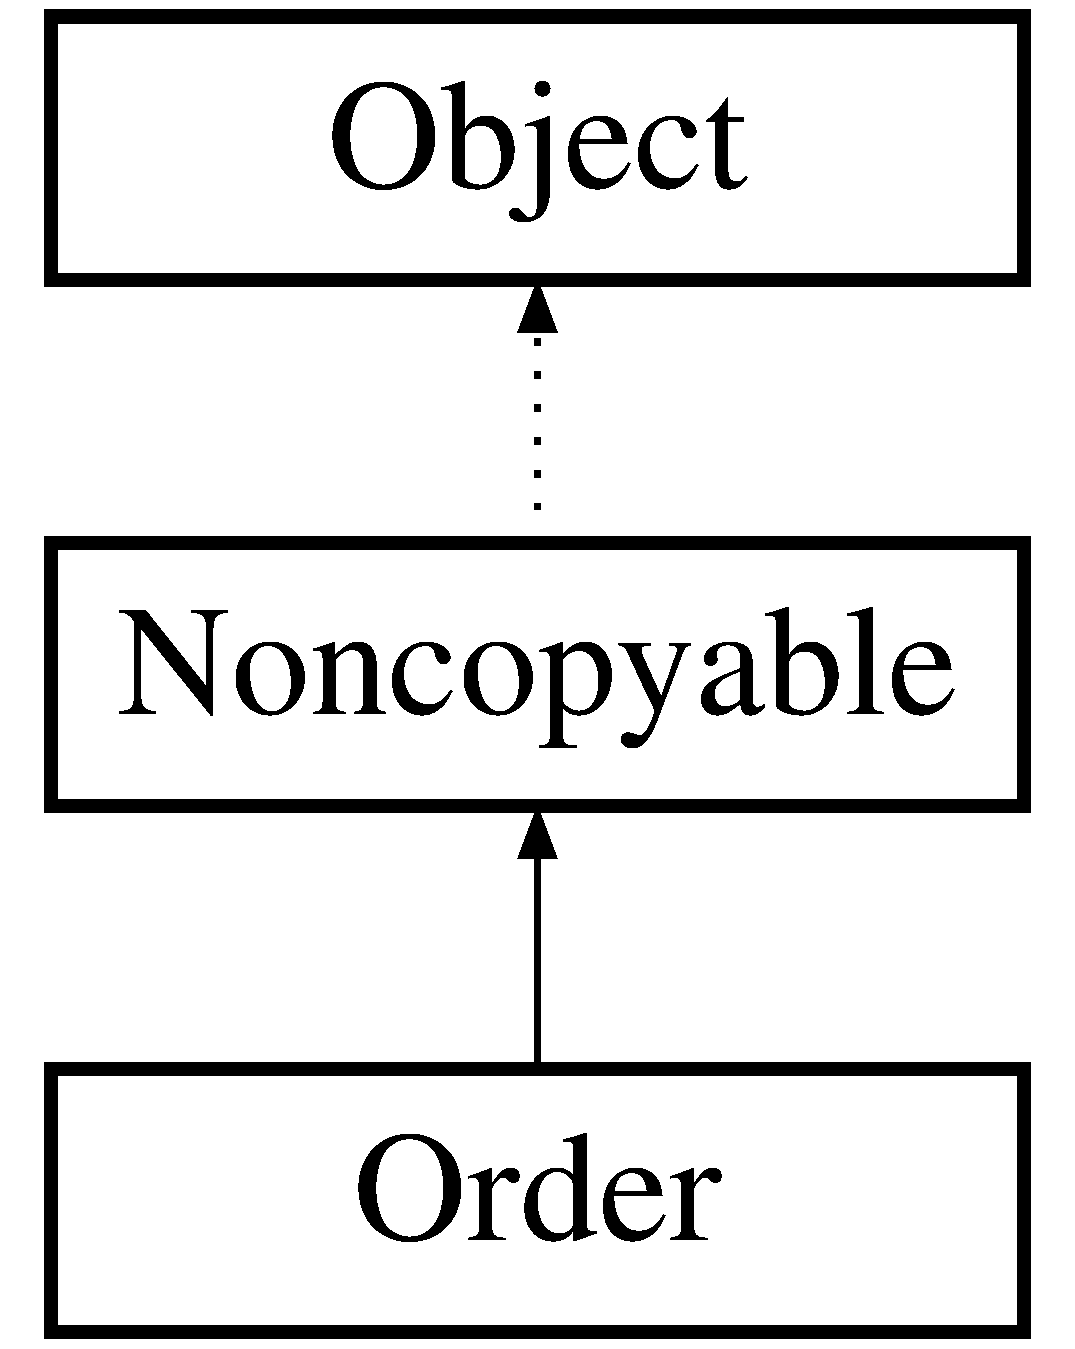
\includegraphics[height=3.000000cm]{classOrder}
\end{center}
\end{figure}
\subsection*{Public Member Functions}
\begin{DoxyCompactItemize}
\item 
\hypertarget{classOrder_ae188d30917a4f10444d428e6bfafe8ac}{}\label{classOrder_ae188d30917a4f10444d428e6bfafe8ac} 
{\bfseries Order} (\hyperlink{classOrder}{Order} \&\&other)
\item 
\hypertarget{classOrder_a07e33dd146779382d4f7321e1ae4d505}{}\label{classOrder_a07e33dd146779382d4f7321e1ae4d505} 
\hyperlink{classOrder_a07e33dd146779382d4f7321e1ae4d505}{Order} (const int n)
\begin{DoxyCompactList}\small\item\em Construct identity of given size. \end{DoxyCompactList}\item 
\hypertarget{classOrder_ab6b1af85c1a2f67023b46bae2beaacf9}{}\label{classOrder_ab6b1af85c1a2f67023b46bae2beaacf9} 
\hyperlink{classOrder}{Order} \& {\bfseries operator=} (\hyperlink{classOrder}{Order} \&\&other)
\item 
\hypertarget{classOrder_a337740020faa60244d7103d839465014}{}\label{classOrder_a337740020faa60244d7103d839465014} 
{\footnotesize template$<$typename T\+Comparator $>$ }\\void \hyperlink{classOrder_a337740020faa60244d7103d839465014}{shuffle} (T\+Comparator \&\&comparator)
\begin{DoxyCompactList}\small\item\em Shuffle order by given comparator. \end{DoxyCompactList}\item 
\hypertarget{classOrder_abfb5b149c5993d6a99c50a847fe92414}{}\label{classOrder_abfb5b149c5993d6a99c50a847fe92414} 
\hyperlink{classOrder}{Order} \hyperlink{classOrder_abfb5b149c5993d6a99c50a847fe92414}{get\+Inverted} () const
\begin{DoxyCompactList}\small\item\em Returns inverted order. \end{DoxyCompactList}\item 
\hypertarget{classOrder_ad5c943d3d8f6aafe3f8a0e0489b9a039}{}\label{classOrder_ad5c943d3d8f6aafe3f8a0e0489b9a039} 
\hyperlink{classOrder}{Order} \hyperlink{classOrder_ad5c943d3d8f6aafe3f8a0e0489b9a039}{operator()} (const \hyperlink{classOrder}{Order} \&other) const
\begin{DoxyCompactList}\small\item\em Compose two orders. \end{DoxyCompactList}\item 
\hypertarget{classOrder_a2c1ba475a03c4429d996361c2e02690f}{}\label{classOrder_a2c1ba475a03c4429d996361c2e02690f} 
I\+N\+L\+I\+NE int {\bfseries operator\mbox{[}$\,$\mbox{]}} (const int idx) const
\item 
\hypertarget{classOrder_a3a1b73d68ad74b75e18a57aaccc060cc}{}\label{classOrder_a3a1b73d68ad74b75e18a57aaccc060cc} 
I\+N\+L\+I\+NE bool {\bfseries operator==} (const \hyperlink{classOrder}{Order} \&other) const
\end{DoxyCompactItemize}


\subsection{Detailed Description}
Permutation, i.\+e. (discrete) invertible function int-\/$>$int. Simple wrapper of \hyperlink{classArray}{Array$<$int$>$} with convenient interface that guarantees the object will be always valid permutation. Only way to modify the object is via {\ttfamily shuffle} function. 

The documentation for this class was generated from the following file\+:\begin{DoxyCompactItemize}
\item 
/home/pavel/projects/astro/sph2/src/tree/order.\+h\end{DoxyCompactItemize}

\hypertarget{classPointCloud}{}\section{Point\+Cloud Class Reference}
\label{classPointCloud}\index{Point\+Cloud@{Point\+Cloud}}


\hyperlink{classArray}{Array} of vectors to be used in nanoflann code.  




{\ttfamily \#include $<$kdtree.\+h$>$}

Inheritance diagram for Point\+Cloud\+:\begin{figure}[H]
\begin{center}
\leavevmode
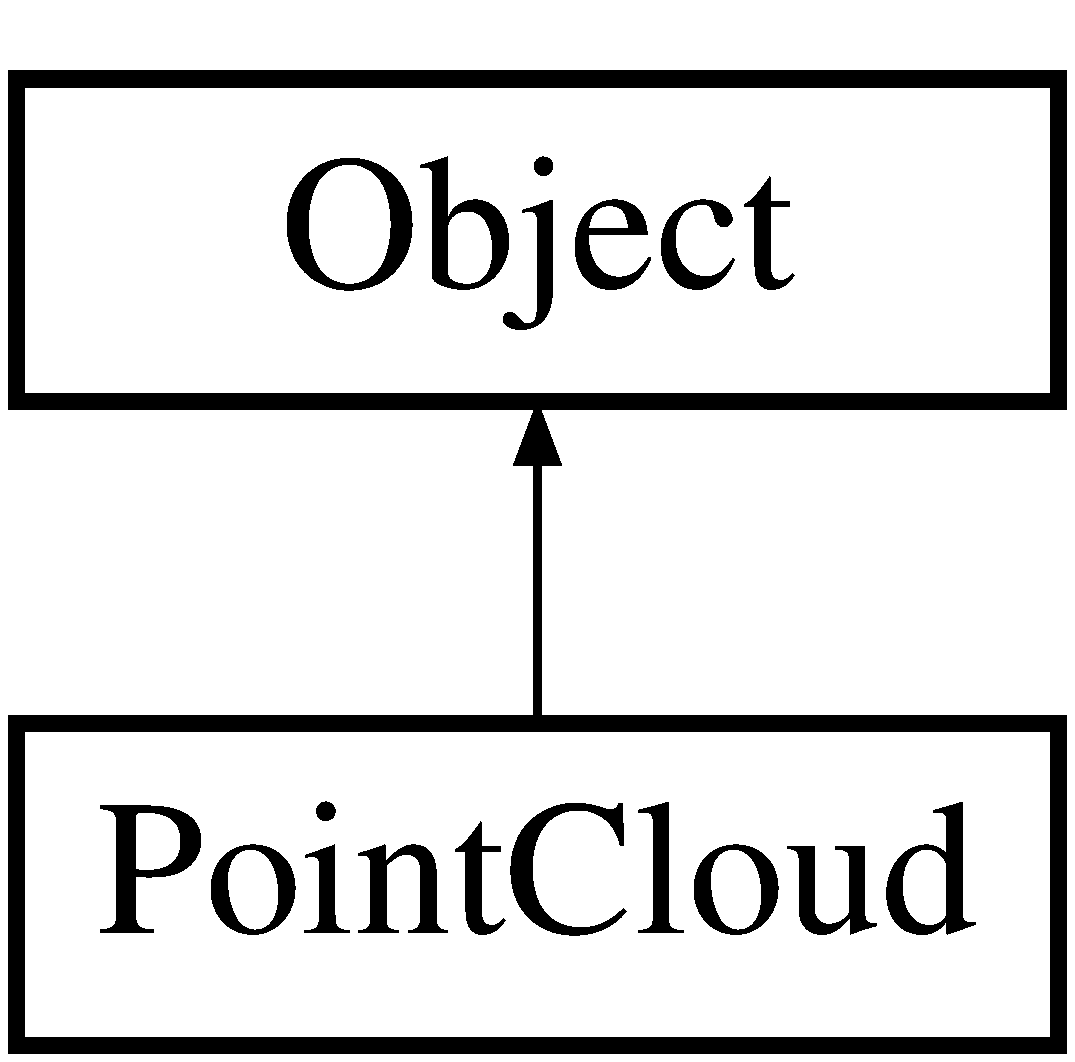
\includegraphics[height=2.000000cm]{classPointCloud}
\end{center}
\end{figure}
\subsection*{Public Member Functions}
\begin{DoxyCompactItemize}
\item 
\hypertarget{classPointCloud_a4ad620d47bd52a25d3eb1e3b0fc0528b}{}\label{classPointCloud_a4ad620d47bd52a25d3eb1e3b0fc0528b} 
{\bfseries Point\+Cloud} (\hyperlink{classArrayView}{Array\+View}$<$ \hyperlink{classBasicVector}{Vector} $>$ storage)
\item 
\hypertarget{classPointCloud_a4fcb3a84da1fae67d4a8812b075b4f14}{}\label{classPointCloud_a4fcb3a84da1fae67d4a8812b075b4f14} 
I\+N\+L\+I\+NE int {\bfseries kdtree\+\_\+get\+\_\+point\+\_\+count} () const
\item 
\hypertarget{classPointCloud_a51d0dbdd3a8425c7f451df7a5f7a91df}{}\label{classPointCloud_a51d0dbdd3a8425c7f451df7a5f7a91df} 
I\+N\+L\+I\+NE Float {\bfseries kdtree\+\_\+distance} (const \hyperlink{classBasicVector}{Vector} \&p1, const int idx2, int U\+N\+U\+S\+ED(size)) const
\item 
\hypertarget{classPointCloud_a87744cb85ba9aa2c0975fe6e6d3f7a1e}{}\label{classPointCloud_a87744cb85ba9aa2c0975fe6e6d3f7a1e} 
I\+N\+L\+I\+NE Float {\bfseries kdtree\+\_\+get\+\_\+pt} (const int idx, int n) const
\item 
\hypertarget{classPointCloud_a900fa261a2708f48cc6c1e9411755d3e}{}\label{classPointCloud_a900fa261a2708f48cc6c1e9411755d3e} 
{\footnotesize template$<$class B\+B\+OX $>$ }\\bool {\bfseries kdtree\+\_\+get\+\_\+bbox} (B\+B\+OX \&U\+N\+U\+S\+ED(bb)) const
\end{DoxyCompactItemize}


\subsection{Detailed Description}
\hyperlink{classArray}{Array} of vectors to be used in nanoflann code. 

The documentation for this class was generated from the following file\+:\begin{DoxyCompactItemize}
\item 
/home/pavel/projects/astro/sph2/src/tree/kdtree.\+h\end{DoxyCompactItemize}

\hypertarget{classPolymorphic}{}\section{Polymorphic Class Reference}
\label{classPolymorphic}\index{Polymorphic@{Polymorphic}}
Inheritance diagram for Polymorphic\+:\begin{figure}[H]
\begin{center}
\leavevmode
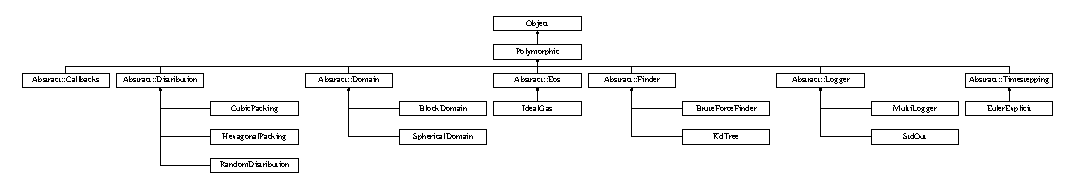
\includegraphics[height=2.092154cm]{classPolymorphic}
\end{center}
\end{figure}


The documentation for this class was generated from the following file\+:\begin{DoxyCompactItemize}
\item 
/home/pavel/projects/astro/sph2/src/core/object.\+h\end{DoxyCompactItemize}

\hypertarget{classSph_1_1PooledAllocator}{}\section{Sph\+:\+:Pooled\+Allocator Class Reference}
\label{classSph_1_1PooledAllocator}\index{Sph\+::\+Pooled\+Allocator@{Sph\+::\+Pooled\+Allocator}}
\subsection*{Public Member Functions}
\begin{DoxyCompactItemize}
\item 
\hyperlink{classSph_1_1PooledAllocator_a88e0fa5e5936ff3b8041dd219de17553}{Pooled\+Allocator} ()
\item 
\hyperlink{classSph_1_1PooledAllocator_a4a29f040cee13bd4a118bd31d762c8fb}{$\sim$\+Pooled\+Allocator} ()
\item 
void \hyperlink{classSph_1_1PooledAllocator_aba832ee65b680cd0b128471fedc749df}{free\+\_\+all} ()
\item 
void $\ast$ \hyperlink{classSph_1_1PooledAllocator_a9a9976d06e621b3f2815538c01c1ca26}{malloc} (const size\+\_\+t req\+\_\+size)
\item 
{\footnotesize template$<$typename T $>$ }\\T $\ast$ \hyperlink{classSph_1_1PooledAllocator_a7c9d02c5d34a4e6cb0393d78a978c56f}{allocate} (const size\+\_\+t count=1)
\end{DoxyCompactItemize}
\subsection*{Public Attributes}
\begin{DoxyCompactItemize}
\item 
\hypertarget{classSph_1_1PooledAllocator_a56bbf2a5148e2fafe16fe0429cde7d81}{}\label{classSph_1_1PooledAllocator_a56bbf2a5148e2fafe16fe0429cde7d81} 
size\+\_\+t {\bfseries used\+Memory}
\item 
\hypertarget{classSph_1_1PooledAllocator_af1a82cde8e5659734fde3ada52e3f9dc}{}\label{classSph_1_1PooledAllocator_af1a82cde8e5659734fde3ada52e3f9dc} 
size\+\_\+t {\bfseries wasted\+Memory}
\end{DoxyCompactItemize}


\subsection{Constructor \& Destructor Documentation}
\hypertarget{classSph_1_1PooledAllocator_a88e0fa5e5936ff3b8041dd219de17553}{}\label{classSph_1_1PooledAllocator_a88e0fa5e5936ff3b8041dd219de17553} 
\index{Sph\+::\+Pooled\+Allocator@{Sph\+::\+Pooled\+Allocator}!Pooled\+Allocator@{Pooled\+Allocator}}
\index{Pooled\+Allocator@{Pooled\+Allocator}!Sph\+::\+Pooled\+Allocator@{Sph\+::\+Pooled\+Allocator}}
\subsubsection{\texorpdfstring{Pooled\+Allocator()}{PooledAllocator()}}
{\footnotesize\ttfamily Sph\+::\+Pooled\+Allocator\+::\+Pooled\+Allocator (\begin{DoxyParamCaption}{ }\end{DoxyParamCaption})\hspace{0.3cm}{\ttfamily [inline]}}

Default constructor. Initializes a new pool. \hypertarget{classSph_1_1PooledAllocator_a4a29f040cee13bd4a118bd31d762c8fb}{}\label{classSph_1_1PooledAllocator_a4a29f040cee13bd4a118bd31d762c8fb} 
\index{Sph\+::\+Pooled\+Allocator@{Sph\+::\+Pooled\+Allocator}!````~Pooled\+Allocator@{$\sim$\+Pooled\+Allocator}}
\index{````~Pooled\+Allocator@{$\sim$\+Pooled\+Allocator}!Sph\+::\+Pooled\+Allocator@{Sph\+::\+Pooled\+Allocator}}
\subsubsection{\texorpdfstring{$\sim$\+Pooled\+Allocator()}{~PooledAllocator()}}
{\footnotesize\ttfamily Sph\+::\+Pooled\+Allocator\+::$\sim$\+Pooled\+Allocator (\begin{DoxyParamCaption}{ }\end{DoxyParamCaption})\hspace{0.3cm}{\ttfamily [inline]}}

Destructor. Frees all the memory allocated in this pool. 

\subsection{Member Function Documentation}
\hypertarget{classSph_1_1PooledAllocator_a7c9d02c5d34a4e6cb0393d78a978c56f}{}\label{classSph_1_1PooledAllocator_a7c9d02c5d34a4e6cb0393d78a978c56f} 
\index{Sph\+::\+Pooled\+Allocator@{Sph\+::\+Pooled\+Allocator}!allocate@{allocate}}
\index{allocate@{allocate}!Sph\+::\+Pooled\+Allocator@{Sph\+::\+Pooled\+Allocator}}
\subsubsection{\texorpdfstring{allocate()}{allocate()}}
{\footnotesize\ttfamily template$<$typename T $>$ \\
T$\ast$ Sph\+::\+Pooled\+Allocator\+::allocate (\begin{DoxyParamCaption}\item[{const size\+\_\+t}]{count = {\ttfamily 1} }\end{DoxyParamCaption})\hspace{0.3cm}{\ttfamily [inline]}}

Allocates (using this pool) a generic type T.

Params\+: count = number of instances to allocate. Returns\+: pointer (of type T$\ast$) to memory buffer \hypertarget{classSph_1_1PooledAllocator_aba832ee65b680cd0b128471fedc749df}{}\label{classSph_1_1PooledAllocator_aba832ee65b680cd0b128471fedc749df} 
\index{Sph\+::\+Pooled\+Allocator@{Sph\+::\+Pooled\+Allocator}!free\+\_\+all@{free\+\_\+all}}
\index{free\+\_\+all@{free\+\_\+all}!Sph\+::\+Pooled\+Allocator@{Sph\+::\+Pooled\+Allocator}}
\subsubsection{\texorpdfstring{free\+\_\+all()}{free\_all()}}
{\footnotesize\ttfamily void Sph\+::\+Pooled\+Allocator\+::free\+\_\+all (\begin{DoxyParamCaption}{ }\end{DoxyParamCaption})\hspace{0.3cm}{\ttfamily [inline]}}

Frees all allocated memory chunks \hypertarget{classSph_1_1PooledAllocator_a9a9976d06e621b3f2815538c01c1ca26}{}\label{classSph_1_1PooledAllocator_a9a9976d06e621b3f2815538c01c1ca26} 
\index{Sph\+::\+Pooled\+Allocator@{Sph\+::\+Pooled\+Allocator}!malloc@{malloc}}
\index{malloc@{malloc}!Sph\+::\+Pooled\+Allocator@{Sph\+::\+Pooled\+Allocator}}
\subsubsection{\texorpdfstring{malloc()}{malloc()}}
{\footnotesize\ttfamily void$\ast$ Sph\+::\+Pooled\+Allocator\+::malloc (\begin{DoxyParamCaption}\item[{const size\+\_\+t}]{req\+\_\+size }\end{DoxyParamCaption})\hspace{0.3cm}{\ttfamily [inline]}}

Returns a pointer to a piece of new memory of the given size in bytes allocated from the pool. 

The documentation for this class was generated from the following file\+:\begin{DoxyCompactItemize}
\item 
/home/pavel/projects/astro/sph2/src/tree/nanoflann.\+h\end{DoxyCompactItemize}

\hypertarget{structMath_1_1Pow}{}\section{Math\+:\+:Pow$<$ d, typename $>$ Struct Template Reference}
\label{structMath_1_1Pow}\index{Math\+::\+Pow$<$ d, typename $>$@{Math\+::\+Pow$<$ d, typename $>$}}
\subsection*{Static Public Member Functions}
\begin{DoxyCompactItemize}
\item 
\hypertarget{structMath_1_1Pow_ac06aece9a0c5dde764987d3e048a9ab3}{}\label{structMath_1_1Pow_ac06aece9a0c5dde764987d3e048a9ab3} 
{\footnotesize template$<$typename T $>$ }\\static I\+N\+L\+I\+NE auto {\bfseries value} (T \&\&v)
\end{DoxyCompactItemize}


The documentation for this struct was generated from the following file\+:\begin{DoxyCompactItemize}
\item 
/home/pavel/projects/astro/sph2/src/core/math.\+h\end{DoxyCompactItemize}

\hypertarget{structMath_1_1Pow_3_010_01_4}{}\section{Math\+:\+:Pow$<$ 0 $>$ Struct Template Reference}
\label{structMath_1_1Pow_3_010_01_4}\index{Math\+::\+Pow$<$ 0 $>$@{Math\+::\+Pow$<$ 0 $>$}}


{\ttfamily \#include $<$math.\+h$>$}

\subsection*{Static Public Member Functions}
\begin{DoxyCompactItemize}
\item 
\hypertarget{structMath_1_1Pow_3_010_01_4_adf20cf05e7a5795a759085c9ee373c62}{}\label{structMath_1_1Pow_3_010_01_4_adf20cf05e7a5795a759085c9ee373c62} 
{\footnotesize template$<$typename T $>$ }\\static I\+N\+L\+I\+NE auto {\bfseries value} (T \&\&U\+N\+U\+S\+ED(v))
\end{DoxyCompactItemize}


\subsection{Detailed Description}
\subsubsection*{template$<$$>$\newline
struct Math\+::\+Pow$<$ 0 $>$}

\begin{DoxyRefDesc}{Todo}
\item[\hyperlink{todo__todo000004}{Todo}]maybe specialize first few pow-\/s to avoid recursion for small values of exponent? \end{DoxyRefDesc}


The documentation for this struct was generated from the following file\+:\begin{DoxyCompactItemize}
\item 
/home/pavel/projects/astro/sph2/src/core/math.\+h\end{DoxyCompactItemize}

\hypertarget{structPowerType}{}\section{Power\+Type$<$ T, n $>$ Struct Template Reference}
\label{structPowerType}\index{Power\+Type$<$ T, n $>$@{Power\+Type$<$ T, n $>$}}


n-\/th power of a quantity  




{\ttfamily \#include $<$traits.\+h$>$}

\subsection*{Public Types}
\begin{DoxyCompactItemize}
\item 
\hypertarget{structPowerType_a4624d6c33f7b9ede7292a0d3aa04f1f4}{}\label{structPowerType_a4624d6c33f7b9ede7292a0d3aa04f1f4} 
using {\bfseries Type} = T
\end{DoxyCompactItemize}


\subsection{Detailed Description}
\subsubsection*{template$<$typename T, int n$>$\newline
struct Power\+Type$<$ T, n $>$}

n-\/th power of a quantity 

The documentation for this struct was generated from the following file\+:\begin{DoxyCompactItemize}
\item 
/home/pavel/projects/astro/sph2/src/core/traits.\+h\end{DoxyCompactItemize}

\hypertarget{classProblem}{}\section{Problem$<$ T\+Model $>$ Class Template Reference}
\label{classProblem}\index{Problem$<$ T\+Model $>$@{Problem$<$ T\+Model $>$}}


{\ttfamily \#include $<$core.\+h$>$}

Inheritance diagram for Problem$<$ T\+Model $>$\+:\begin{figure}[H]
\begin{center}
\leavevmode
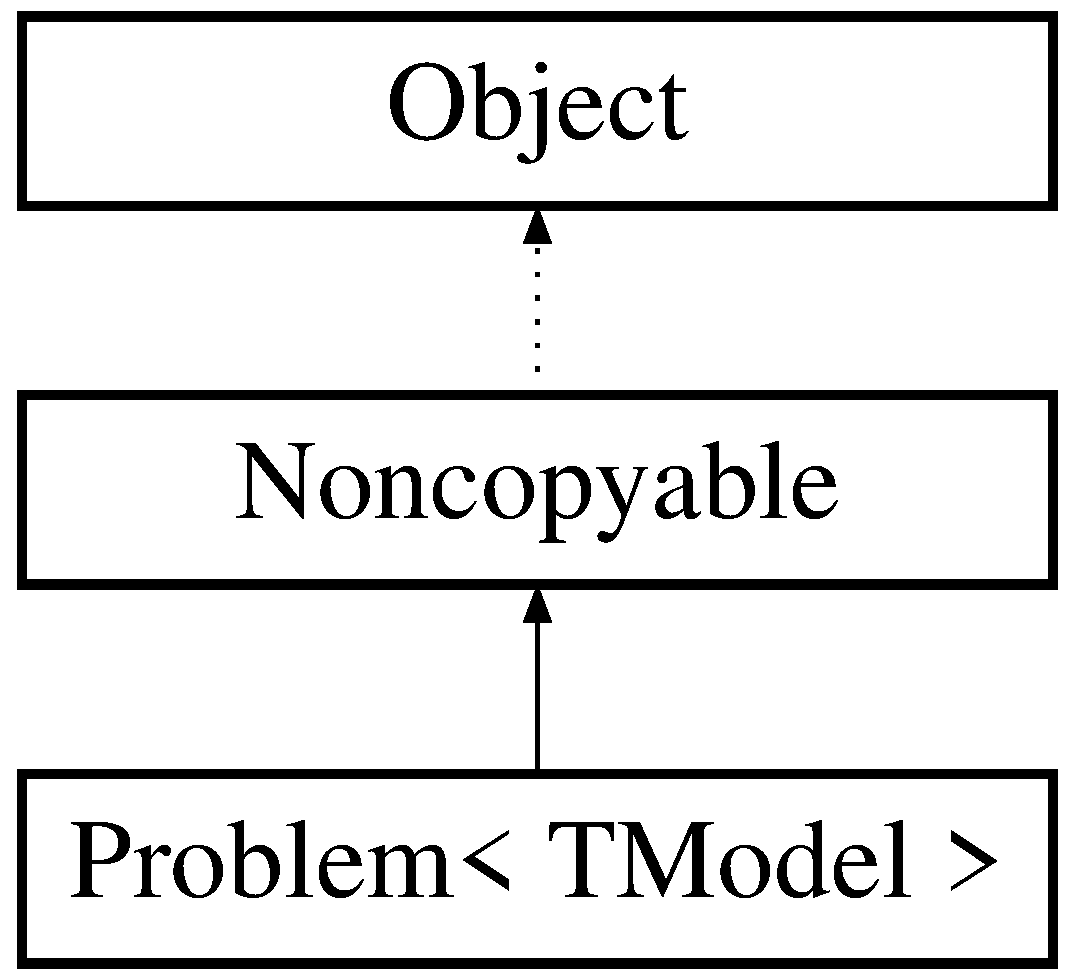
\includegraphics[height=3.000000cm]{classProblem}
\end{center}
\end{figure}
\subsection*{Public Member Functions}
\begin{DoxyCompactItemize}
\item 
void \hyperlink{classProblem_a27fca73edfbe372285fefc86f56d2718}{init} (const int n, \hyperlink{classAbstract_1_1Distribution}{Abstract\+::\+Distribution} $\ast$distribution)
\item 
void \hyperlink{classProblem_a8e9921afda2d764af0e04fe0e632f993}{run} ()
\end{DoxyCompactItemize}
\subsection*{Public Attributes}
\begin{DoxyCompactItemize}
\item 
\hypertarget{classProblem_aff927e5e10d30c96710807d1462476b4}{}\label{classProblem_aff927e5e10d30c96710807d1462476b4} 
\hyperlink{classLutKernel}{Lut\+Kernel} \hyperlink{classProblem_aff927e5e10d30c96710807d1462476b4}{kernel}
\begin{DoxyCompactList}\small\item\em Selected kernel for S\+PH computations. \end{DoxyCompactList}\item 
\hypertarget{classProblem_a6895f42599f432d175a96fbc48e5dcbf}{}\label{classProblem_a6895f42599f432d175a96fbc48e5dcbf} 
std\+::unique\+\_\+ptr$<$ \hyperlink{classAbstract_1_1Finder}{Abstract\+::\+Finder} $>$ \hyperlink{classProblem_a6895f42599f432d175a96fbc48e5dcbf}{finder}
\begin{DoxyCompactList}\small\item\em Structure for k-\/\+NN range-\/limited queries. \end{DoxyCompactList}\item 
\hypertarget{classProblem_a14657abcb68541eaee89483d8086d66d}{}\label{classProblem_a14657abcb68541eaee89483d8086d66d} 
std\+::unique\+\_\+ptr$<$ \hyperlink{classAbstract_1_1Domain}{Abstract\+::\+Domain} $>$ \hyperlink{classProblem_a14657abcb68541eaee89483d8086d66d}{domain}
\begin{DoxyCompactList}\small\item\em Selected computational domain. \end{DoxyCompactList}\item 
\hypertarget{classProblem_ac7ea807f825bf095e17ca55c4236a716}{}\label{classProblem_ac7ea807f825bf095e17ca55c4236a716} 
std\+::unique\+\_\+ptr$<$ \hyperlink{classAbstract_1_1Timestepping}{Abstract\+::\+Timestepping} $>$ \hyperlink{classProblem_ac7ea807f825bf095e17ca55c4236a716}{timestepping}
\begin{DoxyCompactList}\small\item\em Timestepping algorithm. \end{DoxyCompactList}\item 
\hypertarget{classProblem_a61d1fdc0e919a281b8b547fb2765daee}{}\label{classProblem_a61d1fdc0e919a281b8b547fb2765daee} 
std\+::unique\+\_\+ptr$<$ \hyperlink{classAbstract_1_1Logger}{Abstract\+::\+Logger} $>$ \hyperlink{classProblem_a61d1fdc0e919a281b8b547fb2765daee}{logger}
\begin{DoxyCompactList}\small\item\em Output. \end{DoxyCompactList}\item 
\hypertarget{classProblem_a9eb29a52f06b59e9cf018eb6f8c599ad}{}\label{classProblem_a9eb29a52f06b59e9cf018eb6f8c599ad} 
std\+::unique\+\_\+ptr$<$ \hyperlink{classAbstract_1_1Callbacks}{Abstract\+::\+Callbacks} $>$ \hyperlink{classProblem_a9eb29a52f06b59e9cf018eb6f8c599ad}{callbacks}
\begin{DoxyCompactList}\small\item\em G\+UI callbacks. \end{DoxyCompactList}\item 
\hyperlink{classRange}{Range}$<$ Float $>$ \hyperlink{classProblem_ac375fb4749fa6006cdf4705b238deed9}{time\+Range}
\item 
\hypertarget{classProblem_aaac5f756bcaf526e53d640c6d37d01ce}{}\label{classProblem_aaac5f756bcaf526e53d640c6d37d01ce} 
T\+Model \hyperlink{classProblem_aaac5f756bcaf526e53d640c6d37d01ce}{model}
\begin{DoxyCompactList}\small\item\em All quantities. \end{DoxyCompactList}\end{DoxyCompactItemize}


\subsection{Detailed Description}
\subsubsection*{template$<$typename T\+Model$>$\newline
class Problem$<$ T\+Model $>$}

class Domain\+Enforce ? initial distribution of particles $\sim$ domain nothing ghost particles hard domain (setting positions without interactions) 

\subsection{Member Function Documentation}
\hypertarget{classProblem_a27fca73edfbe372285fefc86f56d2718}{}\label{classProblem_a27fca73edfbe372285fefc86f56d2718} 
\index{Problem@{Problem}!init@{init}}
\index{init@{init}!Problem@{Problem}}
\subsubsection{\texorpdfstring{init()}{init()}}
{\footnotesize\ttfamily template$<$typename T\+Model $>$ \\
void \hyperlink{classProblem}{Problem}$<$ T\+Model $>$\+::init (\begin{DoxyParamCaption}\item[{const int}]{n,  }\item[{\hyperlink{classAbstract_1_1Distribution}{Abstract\+::\+Distribution} $\ast$}]{distribution }\end{DoxyParamCaption})\hspace{0.3cm}{\ttfamily [inline]}}

Generate initial conditions

\begin{DoxyRefDesc}{Todo}
\item[\hyperlink{todo__todo000002}{Todo}]by default smoothing lengths h are generated as for eta = 1, account for different values \end{DoxyRefDesc}
\hypertarget{classProblem_a8e9921afda2d764af0e04fe0e632f993}{}\label{classProblem_a8e9921afda2d764af0e04fe0e632f993} 
\index{Problem@{Problem}!run@{run}}
\index{run@{run}!Problem@{Problem}}
\subsubsection{\texorpdfstring{run()}{run()}}
{\footnotesize\ttfamily template$<$typename T\+Model $>$ \\
void \hyperlink{classProblem}{Problem}$<$ T\+Model $>$\+::run (\begin{DoxyParamCaption}{ }\end{DoxyParamCaption})\hspace{0.3cm}{\ttfamily [inline]}}

Output

Initialize all quantities 

\subsection{Member Data Documentation}
\hypertarget{classProblem_ac375fb4749fa6006cdf4705b238deed9}{}\label{classProblem_ac375fb4749fa6006cdf4705b238deed9} 
\index{Problem@{Problem}!time\+Range@{time\+Range}}
\index{time\+Range@{time\+Range}!Problem@{Problem}}
\subsubsection{\texorpdfstring{time\+Range}{timeRange}}
{\footnotesize\ttfamily template$<$typename T\+Model $>$ \\
\hyperlink{classRange}{Range}$<$Float$>$ \hyperlink{classProblem}{Problem}$<$ T\+Model $>$\+::time\+Range}

Time range of the simulations \begin{DoxyRefDesc}{Todo}
\item[\hyperlink{todo__todo000001}{Todo}]other conditions? For example pressure-\/limited simulations? \end{DoxyRefDesc}


The documentation for this class was generated from the following file\+:\begin{DoxyCompactItemize}
\item 
/home/pavel/projects/astro/sph2/src/core/core.\+h\end{DoxyCompactItemize}

\hypertarget{structProductType}{}\section{Product\+Type$<$ T1, T2 $>$ Struct Template Reference}
\label{structProductType}\index{Product\+Type$<$ T1, T2 $>$@{Product\+Type$<$ T1, T2 $>$}}


Product of two quantities.  




{\ttfamily \#include $<$traits.\+h$>$}

\subsection*{Public Types}
\begin{DoxyCompactItemize}
\item 
\hypertarget{structProductType_a55d10db50cc27a747a2c42cf6b33201d}{}\label{structProductType_a55d10db50cc27a747a2c42cf6b33201d} 
using {\bfseries Type} = decltype(std\+::declval$<$ T1 $>$() $\ast$std\+::declval$<$ T2 $>$())
\end{DoxyCompactItemize}


\subsection{Detailed Description}
\subsubsection*{template$<$typename T1, typename T2$>$\newline
struct Product\+Type$<$ T1, T2 $>$}

Product of two quantities. 

Useful types for functions that change the dimensions of units By default, it is simply the type itself 

The documentation for this struct was generated from the following file\+:\begin{DoxyCompactItemize}
\item 
/home/pavel/projects/astro/sph2/src/core/traits.\+h\end{DoxyCompactItemize}

\hypertarget{structQuotientType}{}\section{Quotient\+Type$<$ T1, T2 $>$ Struct Template Reference}
\label{structQuotientType}\index{Quotient\+Type$<$ T1, T2 $>$@{Quotient\+Type$<$ T1, T2 $>$}}


Ratio of two quantities.  




{\ttfamily \#include $<$traits.\+h$>$}

\subsection*{Public Types}
\begin{DoxyCompactItemize}
\item 
\hypertarget{structQuotientType_ab2538562c0ae0fc232064bfaa50e3990}{}\label{structQuotientType_ab2538562c0ae0fc232064bfaa50e3990} 
using {\bfseries Type} = decltype(std\+::declval$<$ T1 $>$()/std\+::declval$<$ T2 $>$())
\end{DoxyCompactItemize}


\subsection{Detailed Description}
\subsubsection*{template$<$typename T1, typename T2$>$\newline
struct Quotient\+Type$<$ T1, T2 $>$}

Ratio of two quantities. 

The documentation for this struct was generated from the following file\+:\begin{DoxyCompactItemize}
\item 
/home/pavel/projects/astro/sph2/src/core/traits.\+h\end{DoxyCompactItemize}

\hypertarget{classSph_1_1RadiusResultSet}{}\section{Sph\+:\+:Radius\+Result\+Set$<$ Distance\+Type, Index\+Type $>$ Class Template Reference}
\label{classSph_1_1RadiusResultSet}\index{Sph\+::\+Radius\+Result\+Set$<$ Distance\+Type, Index\+Type $>$@{Sph\+::\+Radius\+Result\+Set$<$ Distance\+Type, Index\+Type $>$}}


{\ttfamily \#include $<$nanoflann.\+h$>$}

\subsection*{Public Member Functions}
\begin{DoxyCompactItemize}
\item 
\hypertarget{classSph_1_1RadiusResultSet_a695d4e3b0072d02d431a33b65ce1d9c8}{}\label{classSph_1_1RadiusResultSet_a695d4e3b0072d02d431a33b65ce1d9c8} 
{\bfseries Radius\+Result\+Set} (Distance\+Type radius\+\_\+, \hyperlink{classArray}{Array}$<$ \hyperlink{structNeighbourRecord}{Neighbour\+Record} $>$ \&indices\+\_\+dists)
\item 
\hypertarget{classSph_1_1RadiusResultSet_abb3cd6030f375acc75d6b872db86d1c3}{}\label{classSph_1_1RadiusResultSet_abb3cd6030f375acc75d6b872db86d1c3} 
void {\bfseries init} ()
\item 
\hypertarget{classSph_1_1RadiusResultSet_aa5b31d797a6ee326d4eef489541d0a49}{}\label{classSph_1_1RadiusResultSet_aa5b31d797a6ee326d4eef489541d0a49} 
void {\bfseries clear} ()
\item 
\hypertarget{classSph_1_1RadiusResultSet_a1fc29160438f45e8639c3cc8db6ef174}{}\label{classSph_1_1RadiusResultSet_a1fc29160438f45e8639c3cc8db6ef174} 
size\+\_\+t {\bfseries size} () const
\item 
\hypertarget{classSph_1_1RadiusResultSet_a89c8ebc4c00883b65ee4aa66a2662e66}{}\label{classSph_1_1RadiusResultSet_a89c8ebc4c00883b65ee4aa66a2662e66} 
bool {\bfseries full} () const
\item 
\hypertarget{classSph_1_1RadiusResultSet_a3a733f893b9a991b6d30d6f8c133b6c9}{}\label{classSph_1_1RadiusResultSet_a3a733f893b9a991b6d30d6f8c133b6c9} 
void {\bfseries add\+Point} (Distance\+Type dist, Index\+Type index)
\item 
\hypertarget{classSph_1_1RadiusResultSet_a2a0d506ca93863bdfa7cb36d6db69fa9}{}\label{classSph_1_1RadiusResultSet_a2a0d506ca93863bdfa7cb36d6db69fa9} 
Distance\+Type {\bfseries worst\+Dist} () const
\item 
void \hyperlink{classSph_1_1RadiusResultSet_a50c0144e5989939328fa973cec8c54b6}{set\+\_\+radius\+\_\+and\+\_\+clear} (const Distance\+Type r)
\item 
\hyperlink{structNeighbourRecord}{Neighbour\+Record} \hyperlink{classSph_1_1RadiusResultSet_ac6e69e0729bcdca7191dc0ef92b98797}{worst\+\_\+item} () const
\end{DoxyCompactItemize}
\subsection*{Public Attributes}
\begin{DoxyCompactItemize}
\item 
\hypertarget{classSph_1_1RadiusResultSet_ab80380d01377ffe8f622e28fb85321f4}{}\label{classSph_1_1RadiusResultSet_ab80380d01377ffe8f622e28fb85321f4} 
const Distance\+Type {\bfseries radius}
\item 
\hypertarget{classSph_1_1RadiusResultSet_ab223584a44ee50d32dd7289d124d8345}{}\label{classSph_1_1RadiusResultSet_ab223584a44ee50d32dd7289d124d8345} 
\hyperlink{classArray}{Array}$<$ \hyperlink{structNeighbourRecord}{Neighbour\+Record} $>$ \& {\bfseries m\+\_\+indices\+\_\+dists}
\end{DoxyCompactItemize}


\subsection{Detailed Description}
\subsubsection*{template$<$typename Distance\+Type, typename Index\+Type = size\+\_\+t$>$\newline
class Sph\+::\+Radius\+Result\+Set$<$ Distance\+Type, Index\+Type $>$}

A result-\/set class used when performing a radius based search. 

\subsection{Member Function Documentation}
\hypertarget{classSph_1_1RadiusResultSet_a50c0144e5989939328fa973cec8c54b6}{}\label{classSph_1_1RadiusResultSet_a50c0144e5989939328fa973cec8c54b6} 
\index{Sph\+::\+Radius\+Result\+Set@{Sph\+::\+Radius\+Result\+Set}!set\+\_\+radius\+\_\+and\+\_\+clear@{set\+\_\+radius\+\_\+and\+\_\+clear}}
\index{set\+\_\+radius\+\_\+and\+\_\+clear@{set\+\_\+radius\+\_\+and\+\_\+clear}!Sph\+::\+Radius\+Result\+Set@{Sph\+::\+Radius\+Result\+Set}}
\subsubsection{\texorpdfstring{set\+\_\+radius\+\_\+and\+\_\+clear()}{set\_radius\_and\_clear()}}
{\footnotesize\ttfamily template$<$typename Distance\+Type, typename Index\+Type = size\+\_\+t$>$ \\
void \hyperlink{classSph_1_1RadiusResultSet}{Sph\+::\+Radius\+Result\+Set}$<$ Distance\+Type, Index\+Type $>$\+::set\+\_\+radius\+\_\+and\+\_\+clear (\begin{DoxyParamCaption}\item[{const Distance\+Type}]{r }\end{DoxyParamCaption})\hspace{0.3cm}{\ttfamily [inline]}}

Clears the result set and adjusts the search radius. \hypertarget{classSph_1_1RadiusResultSet_ac6e69e0729bcdca7191dc0ef92b98797}{}\label{classSph_1_1RadiusResultSet_ac6e69e0729bcdca7191dc0ef92b98797} 
\index{Sph\+::\+Radius\+Result\+Set@{Sph\+::\+Radius\+Result\+Set}!worst\+\_\+item@{worst\+\_\+item}}
\index{worst\+\_\+item@{worst\+\_\+item}!Sph\+::\+Radius\+Result\+Set@{Sph\+::\+Radius\+Result\+Set}}
\subsubsection{\texorpdfstring{worst\+\_\+item()}{worst\_item()}}
{\footnotesize\ttfamily template$<$typename Distance\+Type, typename Index\+Type = size\+\_\+t$>$ \\
\hyperlink{structNeighbourRecord}{Neighbour\+Record} \hyperlink{classSph_1_1RadiusResultSet}{Sph\+::\+Radius\+Result\+Set}$<$ Distance\+Type, Index\+Type $>$\+::worst\+\_\+item (\begin{DoxyParamCaption}{ }\end{DoxyParamCaption}) const\hspace{0.3cm}{\ttfamily [inline]}}

Find the worst result (furtherest neighbor) without copying or sorting Pre-\/conditions\+: size() $>$ 0 

The documentation for this class was generated from the following file\+:\begin{DoxyCompactItemize}
\item 
/home/pavel/projects/astro/sph2/src/tree/nanoflann.\+h\end{DoxyCompactItemize}

\hypertarget{classRandomDistribution}{}\section{Random\+Distribution Class Reference}
\label{classRandomDistribution}\index{Random\+Distribution@{Random\+Distribution}}
Inheritance diagram for Random\+Distribution\+:\begin{figure}[H]
\begin{center}
\leavevmode
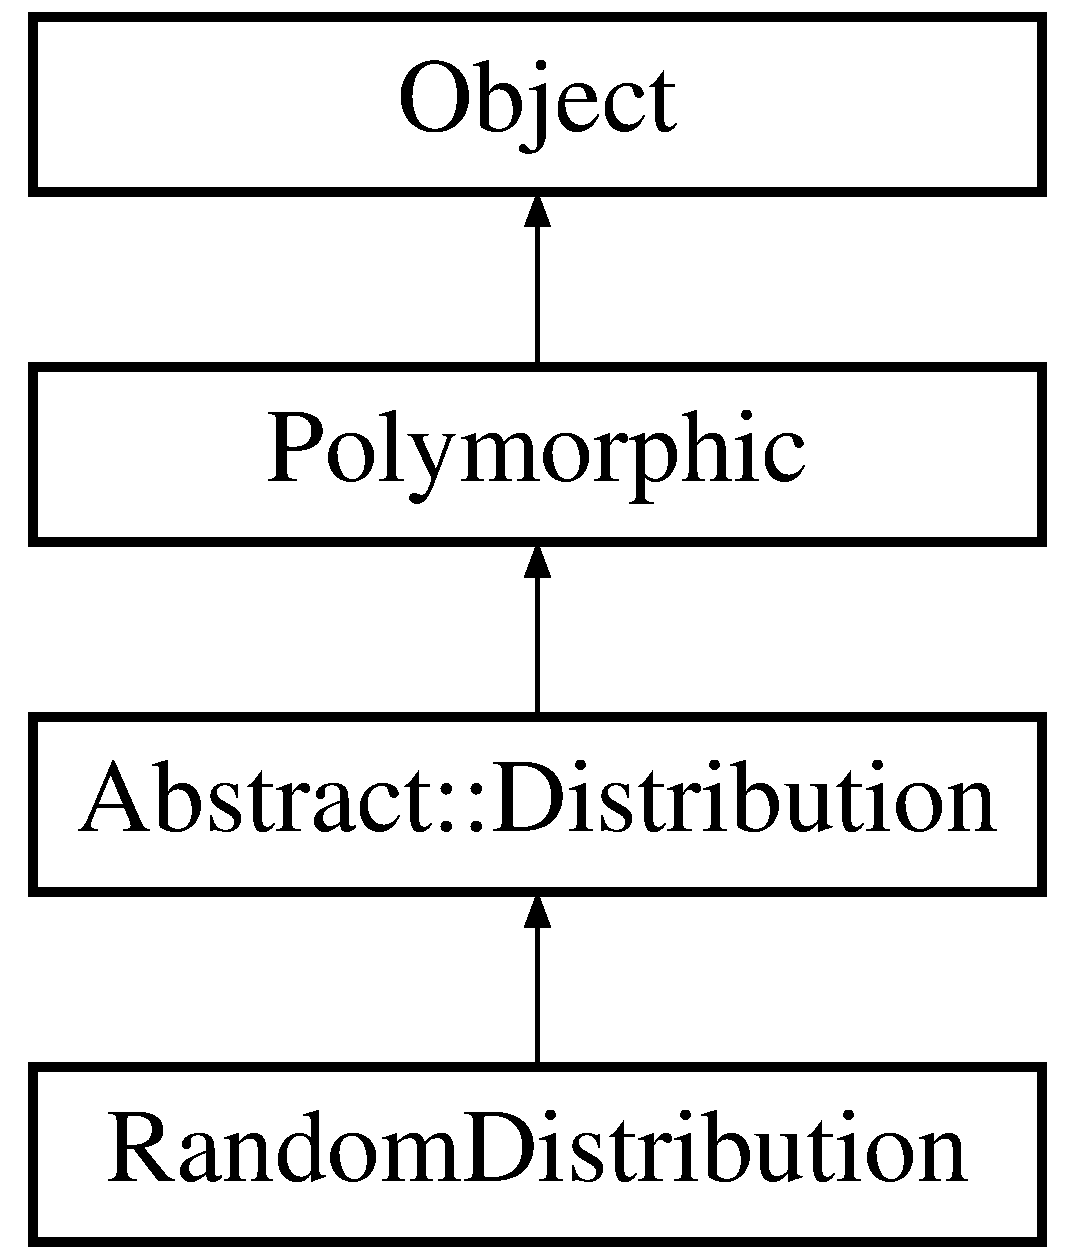
\includegraphics[height=4.000000cm]{classRandomDistribution}
\end{center}
\end{figure}
\subsection*{Public Member Functions}
\begin{DoxyCompactItemize}
\item 
virtual \hyperlink{classArray}{Array}$<$ \hyperlink{classBasicVector}{Vector} $>$ \hyperlink{classRandomDistribution_a3e1308d2bb28c5801e6e0537a8002597}{generate} (const int n, const \hyperlink{classAbstract_1_1Domain}{Abstract\+::\+Domain} $\ast$domain) const override
\end{DoxyCompactItemize}


\subsection{Member Function Documentation}
\hypertarget{classRandomDistribution_a3e1308d2bb28c5801e6e0537a8002597}{}\label{classRandomDistribution_a3e1308d2bb28c5801e6e0537a8002597} 
\index{Random\+Distribution@{Random\+Distribution}!generate@{generate}}
\index{generate@{generate}!Random\+Distribution@{Random\+Distribution}}
\subsubsection{\texorpdfstring{generate()}{generate()}}
{\footnotesize\ttfamily virtual \hyperlink{classArray}{Array}$<$\hyperlink{classBasicVector}{Vector}$>$ Random\+Distribution\+::generate (\begin{DoxyParamCaption}\item[{const int}]{n,  }\item[{const \hyperlink{classAbstract_1_1Domain}{Abstract\+::\+Domain} $\ast$}]{domain }\end{DoxyParamCaption}) const\hspace{0.3cm}{\ttfamily [inline]}, {\ttfamily [override]}, {\ttfamily [virtual]}}

Base class for generating vertices with specific distribution. Also generates corresponding smoothing lengths and save them as fourth component of the vector. 
\begin{DoxyParams}{Parameters}
{\em n} & Expected number of generated vertices. \\
\hline
{\em domain} & Computational domain where the vertices are distributed \\
\hline
\end{DoxyParams}
\begin{DoxyReturn}{Returns}
Output array of vertices. The total number of vertices can slightly differ from n. 
\end{DoxyReturn}
\begin{DoxyNote}{Note}
This method is expected to be called once at the beginning of the run, so we can return allocated array without worrying about performance costs here. 
\end{DoxyNote}


Implements \hyperlink{classAbstract_1_1Distribution_aefb835b4c4d2d0a5f864bc2cee0492b2}{Abstract\+::\+Distribution}.



The documentation for this class was generated from the following file\+:\begin{DoxyCompactItemize}
\item 
/home/pavel/projects/astro/sph2/src/initconds/initconds.\+h\end{DoxyCompactItemize}

\hypertarget{classRange}{}\section{Range$<$ T $>$ Class Template Reference}
\label{classRange}\index{Range$<$ T $>$@{Range$<$ T $>$}}
Inheritance diagram for Range$<$ T $>$\+:\begin{figure}[H]
\begin{center}
\leavevmode
\includegraphics[height=2.000000cm]{classRange}
\end{center}
\end{figure}
\subsection*{Public Member Functions}
\begin{DoxyCompactItemize}
\item 
\hypertarget{classRange_a290eaf342b8335196c3ed8cb99b08bf5}{}\label{classRange_a290eaf342b8335196c3ed8cb99b08bf5} 
I\+N\+L\+I\+NE {\bfseries Range} (const T \&lower, const T \&upper)
\item 
\hypertarget{classRange_a92d6878760432c356fb61ebbefde8b89}{}\label{classRange_a92d6878760432c356fb61ebbefde8b89} 
I\+N\+L\+I\+NE void {\bfseries extend} (const T \&value)
\item 
\hypertarget{classRange_afda3d0ddbcd5cfd1e66d80d2b741c0a8}{}\label{classRange_afda3d0ddbcd5cfd1e66d80d2b741c0a8} 
I\+N\+L\+I\+NE bool {\bfseries contains} (const T \&value) const
\item 
\hypertarget{classRange_a064a8c9ada68b6e70dee234ee7f0595f}{}\label{classRange_a064a8c9ada68b6e70dee234ee7f0595f} 
I\+N\+L\+I\+NE T {\bfseries clamp} (const T \&value) const
\item 
\hypertarget{classRange_a97cdd8f707a0356a38bcb302d253be26}{}\label{classRange_a97cdd8f707a0356a38bcb302d253be26} 
I\+N\+L\+I\+NE const T \& {\bfseries get\+Lower} () const
\item 
\hypertarget{classRange_aef738274a91ebdcaa0e8bccf8753fd9a}{}\label{classRange_aef738274a91ebdcaa0e8bccf8753fd9a} 
I\+N\+L\+I\+NE const T \& {\bfseries get\+Upper} () const
\end{DoxyCompactItemize}


The documentation for this class was generated from the following file\+:\begin{DoxyCompactItemize}
\item 
/home/pavel/projects/astro/sph2/src/structs/range.\+h\end{DoxyCompactItemize}

\hypertarget{classRangeAdapter}{}\section{Range\+Adapter$<$ T, T\+Step $>$ Class Template Reference}
\label{classRangeAdapter}\index{Range\+Adapter$<$ T, T\+Step $>$@{Range\+Adapter$<$ T, T\+Step $>$}}
Inheritance diagram for Range\+Adapter$<$ T, T\+Step $>$\+:\begin{figure}[H]
\begin{center}
\leavevmode
\includegraphics[height=2.000000cm]{classRangeAdapter}
\end{center}
\end{figure}
\subsection*{Public Member Functions}
\begin{DoxyCompactItemize}
\item 
\hypertarget{classRangeAdapter_af126cdb4cd1981498478a9f1c8b1ecc6}{}\label{classRangeAdapter_af126cdb4cd1981498478a9f1c8b1ecc6} 
{\bfseries Range\+Adapter} (const \hyperlink{classRange}{Range}$<$ T $>$ \&range, T\+Step \&\&step)
\item 
\hypertarget{classRangeAdapter_a27b7dce9ff6601b03050dcb5039d17d0}{}\label{classRangeAdapter_a27b7dce9ff6601b03050dcb5039d17d0} 
I\+N\+L\+I\+NE \hyperlink{classRangeIterator}{Range\+Iterator}$<$ T, T\+Step $>$ {\bfseries begin} ()
\item 
\hypertarget{classRangeAdapter_a11c3ceedfc37333ec9e2665250db448a}{}\label{classRangeAdapter_a11c3ceedfc37333ec9e2665250db448a} 
I\+N\+L\+I\+NE \hyperlink{classRangeIterator}{Range\+Iterator}$<$ T, T\+Step $>$ {\bfseries end} ()
\end{DoxyCompactItemize}


The documentation for this class was generated from the following file\+:\begin{DoxyCompactItemize}
\item 
/home/pavel/projects/astro/sph2/src/structs/range.\+h\end{DoxyCompactItemize}

\hypertarget{classRangeIterator}{}\section{Range\+Iterator$<$ T, T\+Step $>$ Class Template Reference}
\label{classRangeIterator}\index{Range\+Iterator$<$ T, T\+Step $>$@{Range\+Iterator$<$ T, T\+Step $>$}}
Inheritance diagram for Range\+Iterator$<$ T, T\+Step $>$\+:\begin{figure}[H]
\begin{center}
\leavevmode
\includegraphics[height=2.000000cm]{classRangeIterator}
\end{center}
\end{figure}
\subsection*{Public Member Functions}
\begin{DoxyCompactItemize}
\item 
\hypertarget{classRangeIterator_acb4c90bda028eede14593ca975c2d6eb}{}\label{classRangeIterator_acb4c90bda028eede14593ca975c2d6eb} 
{\bfseries Range\+Iterator} (const T \&value, T\+Step step)
\item 
\hypertarget{classRangeIterator_ab9e4f0319b8f491422540c0ab7dddd5f}{}\label{classRangeIterator_ab9e4f0319b8f491422540c0ab7dddd5f} 
I\+N\+L\+I\+NE \hyperlink{classRangeIterator}{Range\+Iterator} \& {\bfseries operator++} ()
\item 
\hypertarget{classRangeIterator_a40ba1aab3c499855c66b76e05d3720d3}{}\label{classRangeIterator_a40ba1aab3c499855c66b76e05d3720d3} 
I\+N\+L\+I\+NE T \& {\bfseries operator$\ast$} ()
\item 
\hypertarget{classRangeIterator_ad87df1fab2105e31f776ec90ef94ab13}{}\label{classRangeIterator_ad87df1fab2105e31f776ec90ef94ab13} 
I\+N\+L\+I\+NE const T \& {\bfseries operator$\ast$} () const
\item 
\hypertarget{classRangeIterator_ad2f5d05eea4c0bfc27bd0b20b793f547}{}\label{classRangeIterator_ad2f5d05eea4c0bfc27bd0b20b793f547} 
bool {\bfseries operator!=} (const \hyperlink{classRangeIterator}{Range\+Iterator} \&other)
\end{DoxyCompactItemize}


The documentation for this class was generated from the following file\+:\begin{DoxyCompactItemize}
\item 
/home/pavel/projects/astro/sph2/src/structs/range.\+h\end{DoxyCompactItemize}

\hypertarget{structRootType}{}\section{Root\+Type$<$ T, n $>$ Struct Template Reference}
\label{structRootType}\index{Root\+Type$<$ T, n $>$@{Root\+Type$<$ T, n $>$}}


n-\/th root of a quantity  




{\ttfamily \#include $<$traits.\+h$>$}

\subsection*{Public Types}
\begin{DoxyCompactItemize}
\item 
\hypertarget{structRootType_a400498e4fac7797fdae5e7e8ea39015f}{}\label{structRootType_a400498e4fac7797fdae5e7e8ea39015f} 
using {\bfseries Type} = T
\end{DoxyCompactItemize}


\subsection{Detailed Description}
\subsubsection*{template$<$typename T, int n$>$\newline
struct Root\+Type$<$ T, n $>$}

n-\/th root of a quantity 

The documentation for this struct was generated from the following file\+:\begin{DoxyCompactItemize}
\item 
/home/pavel/projects/astro/sph2/src/core/traits.\+h\end{DoxyCompactItemize}

\hypertarget{structSaveArraysImpl}{}\section{Save\+Arrays\+Impl$<$ T0, TS $>$ Struct Template Reference}
\label{structSaveArraysImpl}\index{Save\+Arrays\+Impl$<$ T0, T\+S $>$@{Save\+Arrays\+Impl$<$ T0, T\+S $>$}}
\subsection*{Static Public Member Functions}
\begin{DoxyCompactItemize}
\item 
\hypertarget{structSaveArraysImpl_a96e39c817382fbb444ed8d2fa7e2d7f0}{}\label{structSaveArraysImpl_a96e39c817382fbb444ed8d2fa7e2d7f0} 
static void {\bfseries action} (const std\+::string \&path, const \hyperlink{classArray}{Array}$<$ T0 $>$ \&array, const \hyperlink{classArray}{Array}$<$ TS $>$ \&... others)
\item 
\hypertarget{structSaveArraysImpl_aa7ece4317c14bfdd58452964ca1cdca9}{}\label{structSaveArraysImpl_aa7ece4317c14bfdd58452964ca1cdca9} 
static void {\bfseries print\+Line} (std\+::ofstream \&ofs, const int line, const \hyperlink{classArray}{Array}$<$ T0 $>$ \&array, const \hyperlink{classArray}{Array}$<$ TS $>$ \&... others)
\end{DoxyCompactItemize}


The documentation for this struct was generated from the following file\+:\begin{DoxyCompactItemize}
\item 
/home/pavel/projects/astro/sph2/src/parser/parse.\+h\end{DoxyCompactItemize}

\hypertarget{structSaveArraysImpl_3_01T0_01_4}{}\section{Save\+Arrays\+Impl$<$ T0 $>$ Struct Template Reference}
\label{structSaveArraysImpl_3_01T0_01_4}\index{Save\+Arrays\+Impl$<$ T0 $>$@{Save\+Arrays\+Impl$<$ T0 $>$}}
\subsection*{Static Public Member Functions}
\begin{DoxyCompactItemize}
\item 
\hypertarget{structSaveArraysImpl_3_01T0_01_4_a51ef3bbc8d19b5fc936d9a0b6283f48e}{}\label{structSaveArraysImpl_3_01T0_01_4_a51ef3bbc8d19b5fc936d9a0b6283f48e} 
static void {\bfseries action} (const std\+::string \&path, const \hyperlink{classArray}{Array}$<$ T0 $>$ \&array)
\item 
\hypertarget{structSaveArraysImpl_3_01T0_01_4_a35e01343cd65c09ca9301a42c29cdf6f}{}\label{structSaveArraysImpl_3_01T0_01_4_a35e01343cd65c09ca9301a42c29cdf6f} 
static void {\bfseries print\+Line} (std\+::ofstream \&ofs, const int line, const \hyperlink{classArray}{Array}$<$ T0 $>$ \&array)
\end{DoxyCompactItemize}


The documentation for this struct was generated from the following file\+:\begin{DoxyCompactItemize}
\item 
/home/pavel/projects/astro/sph2/src/parser/parse.\+h\end{DoxyCompactItemize}

\hypertarget{structSph_1_1SearchParams}{}\section{Sph\+:\+:Search\+Params Struct Reference}
\label{structSph_1_1SearchParams}\index{Sph\+::\+Search\+Params@{Sph\+::\+Search\+Params}}


{\ttfamily \#include $<$nanoflann.\+h$>$}

\subsection*{Public Member Functions}
\begin{DoxyCompactItemize}
\item 
\hyperlink{structSph_1_1SearchParams_a810971e8ebb92129213a5413f5717753}{Search\+Params} (int checks\+\_\+\+I\+G\+N\+O\+R\+E\+D\+\_\+=32, float eps\+\_\+=0, bool sorted\+\_\+=true)
\end{DoxyCompactItemize}
\subsection*{Public Attributes}
\begin{DoxyCompactItemize}
\item 
\hypertarget{structSph_1_1SearchParams_a92f3afd3919379b08bdb3a2c0bb5f1aa}{}\label{structSph_1_1SearchParams_a92f3afd3919379b08bdb3a2c0bb5f1aa} 
int \hyperlink{structSph_1_1SearchParams_a92f3afd3919379b08bdb3a2c0bb5f1aa}{checks}
\begin{DoxyCompactList}\small\item\em Ignored parameter (Kept for compatibility with the F\+L\+A\+NN interface). \end{DoxyCompactList}\item 
\hypertarget{structSph_1_1SearchParams_a6ca37d56508646dfe688cf806b892e53}{}\label{structSph_1_1SearchParams_a6ca37d56508646dfe688cf806b892e53} 
float \hyperlink{structSph_1_1SearchParams_a6ca37d56508646dfe688cf806b892e53}{eps}
\begin{DoxyCompactList}\small\item\em search for eps-\/approximate neighbours (default\+: 0) \end{DoxyCompactList}\item 
\hypertarget{structSph_1_1SearchParams_a4ce5e7d92c7027c4bd2ed5cd0d188ffd}{}\label{structSph_1_1SearchParams_a4ce5e7d92c7027c4bd2ed5cd0d188ffd} 
bool \hyperlink{structSph_1_1SearchParams_a4ce5e7d92c7027c4bd2ed5cd0d188ffd}{sorted}
\begin{DoxyCompactList}\small\item\em only for radius search, require neighbours sorted by distance (default\+: true) \end{DoxyCompactList}\end{DoxyCompactItemize}


\subsection{Detailed Description}
Search options for \hyperlink{classSph_1_1KDTreeSingleIndexAdaptor_a444955d9248884e7fcb1fb238c3b0105}{K\+D\+Tree\+Single\+Index\+Adaptor\+::find\+Neighbors()} 

\subsection{Constructor \& Destructor Documentation}
\hypertarget{structSph_1_1SearchParams_a810971e8ebb92129213a5413f5717753}{}\label{structSph_1_1SearchParams_a810971e8ebb92129213a5413f5717753} 
\index{Sph\+::\+Search\+Params@{Sph\+::\+Search\+Params}!Search\+Params@{Search\+Params}}
\index{Search\+Params@{Search\+Params}!Sph\+::\+Search\+Params@{Sph\+::\+Search\+Params}}
\subsubsection{\texorpdfstring{Search\+Params()}{SearchParams()}}
{\footnotesize\ttfamily Sph\+::\+Search\+Params\+::\+Search\+Params (\begin{DoxyParamCaption}\item[{int}]{checks\+\_\+\+I\+G\+N\+O\+R\+E\+D\+\_\+ = {\ttfamily 32},  }\item[{float}]{eps\+\_\+ = {\ttfamily 0},  }\item[{bool}]{sorted\+\_\+ = {\ttfamily true} }\end{DoxyParamCaption})\hspace{0.3cm}{\ttfamily [inline]}}

Note\+: The first argument (checks\+\_\+\+I\+G\+N\+O\+R\+E\+D\+\_\+) is ignored, but kept for compatibility with the F\+L\+A\+NN interface 

The documentation for this struct was generated from the following file\+:\begin{DoxyCompactItemize}
\item 
/home/pavel/projects/astro/sph2/src/tree/nanoflann.\+h\end{DoxyCompactItemize}

\hypertarget{classSettings}{}\section{Settings$<$ T\+Enum $>$ Class Template Reference}
\label{classSettings}\index{Settings$<$ T\+Enum $>$@{Settings$<$ T\+Enum $>$}}
Inheritance diagram for Settings$<$ T\+Enum $>$\+:\begin{figure}[H]
\begin{center}
\leavevmode
\includegraphics[height=2.000000cm]{classSettings}
\end{center}
\end{figure}
\subsection*{Public Member Functions}
\begin{DoxyCompactItemize}
\item 
\hypertarget{classSettings_a17e41d20319e5cbfcb1d0eedb5d44614}{}\label{classSettings_a17e41d20319e5cbfcb1d0eedb5d44614} 
{\bfseries Settings} (std\+::initializer\+\_\+list$<$ Entry $>$ list)
\item 
\hypertarget{classSettings_a9d923cf0b788195b1b327a41eb3c0322}{}\label{classSettings_a9d923cf0b788195b1b327a41eb3c0322} 
\hyperlink{classSettings}{Settings} \& {\bfseries operator=} (std\+::initializer\+\_\+list$<$ Entry $>$ list)
\item 
\hypertarget{classSettings_a15a2bed9d47783ac2b53079f65984d24}{}\label{classSettings_a15a2bed9d47783ac2b53079f65984d24} 
{\footnotesize template$<$typename T\+Value $>$ }\\void {\bfseries set} (T\+Enum idx, T\+Value \&\&value)
\item 
\hypertarget{classSettings_a83eb52723ff2bdbd5858a732cf6dff68}{}\label{classSettings_a83eb52723ff2bdbd5858a732cf6dff68} 
{\footnotesize template$<$typename T\+Value $>$ }\\\hyperlink{classOptional}{Optional}$<$ T\+Value $>$ {\bfseries get} (T\+Enum idx) const
\item 
\hypertarget{classSettings_ac7f86c77abf3e0bab30fa1573a8785d2}{}\label{classSettings_ac7f86c77abf3e0bab30fa1573a8785d2} 
void {\bfseries save\+To\+File} (const std\+::string \&path) const
\end{DoxyCompactItemize}


The documentation for this class was generated from the following file\+:\begin{DoxyCompactItemize}
\item 
/home/pavel/projects/astro/sph2/src/system/settings.\+h\end{DoxyCompactItemize}

\hypertarget{classShadow}{}\section{Shadow$<$ Type $>$ Class Template Reference}
\label{classShadow}\index{Shadow$<$ Type $>$@{Shadow$<$ Type $>$}}


{\ttfamily \#include $<$shadow.\+h$>$}

Inheritance diagram for Shadow$<$ Type $>$\+:\begin{figure}[H]
\begin{center}
\leavevmode
\includegraphics[height=2.000000cm]{classShadow}
\end{center}
\end{figure}
\subsection*{Public Member Functions}
\begin{DoxyCompactItemize}
\item 
\hypertarget{classShadow_a6b9f4601d139818a05c07fe6d6c732c0}{}\label{classShadow_a6b9f4601d139818a05c07fe6d6c732c0} 
{\footnotesize template$<$typename T0 , typename... T\+Args$>$ }\\void {\bfseries emplace} (T0 \&\&t0, T\+Args \&\&... rest)
\item 
\hypertarget{classShadow_a53136ec46fb68619652ef25bd3fa512b}{}\label{classShadow_a53136ec46fb68619652ef25bd3fa512b} 
void {\bfseries destroy} ()
\item 
\hypertarget{classShadow_abf9c3bfc72664efeb45e720f313dbccc}{}\label{classShadow_abf9c3bfc72664efeb45e720f313dbccc} 
\hyperlink{classShadow_abf9c3bfc72664efeb45e720f313dbccc}{operator Type \&} ()
\begin{DoxyCompactList}\small\item\em Implicit conversion to stored type. \end{DoxyCompactList}\item 
\hypertarget{classShadow_a105a239f6888c7c6a0747dab7e0e9b3d}{}\label{classShadow_a105a239f6888c7c6a0747dab7e0e9b3d} 
\hyperlink{classShadow_a105a239f6888c7c6a0747dab7e0e9b3d}{operator const Type \&} ()
\begin{DoxyCompactList}\small\item\em Implicit conversion to stored type, const version. \end{DoxyCompactList}\item 
\hypertarget{classShadow_ac1e29c2df572ad24e55af67605fda05b}{}\label{classShadow_ac1e29c2df572ad24e55af67605fda05b} 
Type \& \hyperlink{classShadow_ac1e29c2df572ad24e55af67605fda05b}{get} ()
\begin{DoxyCompactList}\small\item\em Return the reference to the stored value. \end{DoxyCompactList}\item 
\hypertarget{classShadow_aaa56a4059c2f050c59fc118ff2c4de23}{}\label{classShadow_aaa56a4059c2f050c59fc118ff2c4de23} 
const Type \& \hyperlink{classShadow_aaa56a4059c2f050c59fc118ff2c4de23}{get} () const
\begin{DoxyCompactList}\small\item\em Returns the reference to the stored value, const version. \end{DoxyCompactList}\item 
\hypertarget{classShadow_a8fead834492f436012800fbc1c959f68}{}\label{classShadow_a8fead834492f436012800fbc1c959f68} 
Type $\ast$ {\bfseries operator-\/$>$} ()
\item 
\hypertarget{classShadow_a029c58f5b34eed75a3302f786291a1d3}{}\label{classShadow_a029c58f5b34eed75a3302f786291a1d3} 
const Type $\ast$ {\bfseries operator-\/$>$} () const
\end{DoxyCompactItemize}


\subsection{Detailed Description}
\subsubsection*{template$<$typename Type$>$\newline
class Shadow$<$ Type $>$}

Simple wrapper of type that sidesteps default construction. \hyperlink{classShadow}{Shadow} objects can be therefore default-\/constructed even if the underlying type does not have default constructor. Stored object can be later constructed by calling {\ttfamily emplace} method. Note that when constructed, it has to be later destroyed by explicitly calling {\ttfamily destroy} method, this is not done automatically! \hyperlink{classShadow}{Shadow} object does NO checks when the stored value is accessed, or whether it is constructed multiple times. This is left to the user. 

The documentation for this class was generated from the following file\+:\begin{DoxyCompactItemize}
\item 
/home/pavel/projects/astro/sph2/src/structs/shadow.\+h\end{DoxyCompactItemize}

\hypertarget{classAbstract_1_1Solver}{}\section{Abstract\+:\+:Solver Class Reference}
\label{classAbstract_1_1Solver}\index{Abstract\+::\+Solver@{Abstract\+::\+Solver}}


The documentation for this class was generated from the following file\+:\begin{DoxyCompactItemize}
\item 
/home/pavel/projects/astro/sph2/src/physics/evolution.\+h\end{DoxyCompactItemize}

\hypertarget{classSphericalDomain}{}\section{Spherical\+Domain Class Reference}
\label{classSphericalDomain}\index{Spherical\+Domain@{Spherical\+Domain}}
Inheritance diagram for Spherical\+Domain\+:\begin{figure}[H]
\begin{center}
\leavevmode
\includegraphics[height=4.000000cm]{classSphericalDomain}
\end{center}
\end{figure}
\subsection*{Public Member Functions}
\begin{DoxyCompactItemize}
\item 
\hypertarget{classSphericalDomain_aa065a14a2c52216a7602ced044e03882}{}\label{classSphericalDomain_aa065a14a2c52216a7602ced044e03882} 
{\bfseries Spherical\+Domain} (const \hyperlink{classBasicVector}{Vector} \&center, const Float \&radius)
\item 
\hypertarget{classSphericalDomain_ae1c88a5c019c868a797e03b411e35dd8}{}\label{classSphericalDomain_ae1c88a5c019c868a797e03b411e35dd8} 
virtual Float \hyperlink{classSphericalDomain_ae1c88a5c019c868a797e03b411e35dd8}{get\+Volume} () const override
\begin{DoxyCompactList}\small\item\em Returns the total d-\/dimensional volume of the domain. \end{DoxyCompactList}\item 
\hypertarget{classSphericalDomain_a5383f0d27d5d3d77cf4d287c6a937a51}{}\label{classSphericalDomain_a5383f0d27d5d3d77cf4d287c6a937a51} 
virtual bool \hyperlink{classSphericalDomain_a5383f0d27d5d3d77cf4d287c6a937a51}{is\+Inside} (const \hyperlink{classBasicVector}{Vector} \&v) const override
\begin{DoxyCompactList}\small\item\em Checks if the vector lies inside the domain. \end{DoxyCompactList}\item 
virtual void \hyperlink{classSphericalDomain_aa5f4f17ecc1fa454da8b30e55bba98bf}{are\+Inside} (const \hyperlink{classArrayView}{Array\+View}$<$ \hyperlink{classBasicVector}{Vector} $>$ vs, \hyperlink{classArrayView}{Array\+View}$<$ bool $>$ output) const override
\item 
\hypertarget{classSphericalDomain_a57524f02db83e73146f6117d25de992c}{}\label{classSphericalDomain_a57524f02db83e73146f6117d25de992c} 
virtual void \hyperlink{classSphericalDomain_a57524f02db83e73146f6117d25de992c}{project} (\hyperlink{classArrayView}{Array\+View}$<$ \hyperlink{classBasicVector}{Vector} $>$ vs) const override
\begin{DoxyCompactList}\small\item\em Projects vectors outside of the domain onto its boundary. Vectors inside the domains are untouched. \end{DoxyCompactList}\end{DoxyCompactItemize}
\subsection*{Additional Inherited Members}


\subsection{Member Function Documentation}
\hypertarget{classSphericalDomain_aa5f4f17ecc1fa454da8b30e55bba98bf}{}\label{classSphericalDomain_aa5f4f17ecc1fa454da8b30e55bba98bf} 
\index{Spherical\+Domain@{Spherical\+Domain}!are\+Inside@{are\+Inside}}
\index{are\+Inside@{are\+Inside}!Spherical\+Domain@{Spherical\+Domain}}
\subsubsection{\texorpdfstring{are\+Inside()}{areInside()}}
{\footnotesize\ttfamily virtual void Spherical\+Domain\+::are\+Inside (\begin{DoxyParamCaption}\item[{const \hyperlink{classArrayView}{Array\+View}$<$ \hyperlink{classBasicVector}{Vector} $>$}]{vs,  }\item[{\hyperlink{classArrayView}{Array\+View}$<$ bool $>$}]{output }\end{DoxyParamCaption}) const\hspace{0.3cm}{\ttfamily [inline]}, {\ttfamily [override]}, {\ttfamily [virtual]}}

Checks if elements of an array are inside the domain. Returns the result as array of bools. \hyperlink{classArray}{Array} must be already allocated and its size must match array vs. 

Implements \hyperlink{classAbstract_1_1Domain_a48ecb4ac3dab5f5a5e2de7b8e8218317}{Abstract\+::\+Domain}.



The documentation for this class was generated from the following file\+:\begin{DoxyCompactItemize}
\item 
/home/pavel/projects/astro/sph2/src/geometry/domain.\+h\end{DoxyCompactItemize}

\hypertarget{classStaticArray}{}\section{Static\+Array$<$ T, N $>$ Class Template Reference}
\label{classStaticArray}\index{Static\+Array$<$ T, N $>$@{Static\+Array$<$ T, N $>$}}
Inheritance diagram for Static\+Array$<$ T, N $>$\+:\begin{figure}[H]
\begin{center}
\leavevmode
\includegraphics[height=3.000000cm]{classStaticArray}
\end{center}
\end{figure}
\subsection*{Public Member Functions}
\begin{DoxyCompactItemize}
\item 
\hypertarget{classStaticArray_a7afc6f3dac246b4b3029d675bafa891a}{}\label{classStaticArray_a7afc6f3dac246b4b3029d675bafa891a} 
{\bfseries Static\+Array} (\hyperlink{classStaticArray}{Static\+Array} \&\&other)
\item 
\hypertarget{classStaticArray_abdb198700bd60f1ca555c289e371c3a1}{}\label{classStaticArray_abdb198700bd60f1ca555c289e371c3a1} 
{\bfseries Static\+Array} (std\+::initializer\+\_\+list$<$ T $>$ list)
\item 
\hypertarget{classStaticArray_aa3336d3e804f1e781373b070db4b8933}{}\label{classStaticArray_aa3336d3e804f1e781373b070db4b8933} 
\hyperlink{classStaticArray}{Static\+Array} \& {\bfseries operator=} (\hyperlink{classStaticArray}{Static\+Array} \&\&other)
\item 
\hypertarget{classStaticArray_a1574a69c6f57ae9a57bc52727b973643}{}\label{classStaticArray_a1574a69c6f57ae9a57bc52727b973643} 
\hyperlink{classStaticArray}{Static\+Array} {\bfseries clone} () const
\item 
\hypertarget{classStaticArray_aa0d12fba9d539098180f62eab4c5dceb}{}\label{classStaticArray_aa0d12fba9d539098180f62eab4c5dceb} 
T \& {\bfseries operator\mbox{[}$\,$\mbox{]}} (const int idx)
\item 
\hypertarget{classStaticArray_a002fe3d95904eeb64527bc4e1cc91e17}{}\label{classStaticArray_a002fe3d95904eeb64527bc4e1cc91e17} 
const T \& {\bfseries operator\mbox{[}$\,$\mbox{]}} (const int idx) const
\item 
\hypertarget{classStaticArray_a370e6c931610ab5e4cbbdbf8b0f34cdb}{}\label{classStaticArray_a370e6c931610ab5e4cbbdbf8b0f34cdb} 
constexpr int {\bfseries get\+Size} () const
\item 
\hypertarget{classStaticArray_a8c1c988b8066d74d2067d42d3b0191db}{}\label{classStaticArray_a8c1c988b8066d74d2067d42d3b0191db} 
\hyperlink{classIterator}{Iterator}$<$ T $>$ {\bfseries begin} ()
\item 
\hypertarget{classStaticArray_a79638947269b15047cb1eaba54c117cf}{}\label{classStaticArray_a79638947269b15047cb1eaba54c117cf} 
\hyperlink{classIterator}{Iterator}$<$ const T $>$ {\bfseries begin} () const
\item 
\hypertarget{classStaticArray_a0efbc4b5730477499d7e4f82a604df16}{}\label{classStaticArray_a0efbc4b5730477499d7e4f82a604df16} 
\hyperlink{classIterator}{Iterator}$<$ T $>$ {\bfseries end} ()
\item 
\hypertarget{classStaticArray_ab534dbf8ab31f24d408627d69e45b9d2}{}\label{classStaticArray_ab534dbf8ab31f24d408627d69e45b9d2} 
\hyperlink{classIterator}{Iterator}$<$ const T $>$ {\bfseries end} () const
\item 
\hypertarget{classStaticArray_a321406d3a975ebc881e17d5ab5638a3f}{}\label{classStaticArray_a321406d3a975ebc881e17d5ab5638a3f} 
{\bfseries operator Array\+View$<$ T $>$} ()
\item 
\hypertarget{classStaticArray_a99becbd90a901d41d69aa0fddc05c341}{}\label{classStaticArray_a99becbd90a901d41d69aa0fddc05c341} 
{\bfseries operator Array\+View$<$ const T $>$} () const
\end{DoxyCompactItemize}


The documentation for this class was generated from the following file\+:\begin{DoxyCompactItemize}
\item 
/home/pavel/projects/astro/sph2/src/structs/array.\+h\end{DoxyCompactItemize}

\hypertarget{classStdOut}{}\section{Std\+Out Class Reference}
\label{classStdOut}\index{Std\+Out@{Std\+Out}}


Standard output logger.  




{\ttfamily \#include $<$logger.\+h$>$}

Inheritance diagram for Std\+Out\+:\begin{figure}[H]
\begin{center}
\leavevmode
\includegraphics[height=4.000000cm]{classStdOut}
\end{center}
\end{figure}
\subsection*{Public Member Functions}
\begin{DoxyCompactItemize}
\item 
\hypertarget{classStdOut_a4f968fcf9158797749c4d8aad2da7ceb}{}\label{classStdOut_a4f968fcf9158797749c4d8aad2da7ceb} 
virtual void {\bfseries write} (const std\+::string \&s) override
\end{DoxyCompactItemize}


\subsection{Detailed Description}
Standard output logger. 

The documentation for this class was generated from the following file\+:\begin{DoxyCompactItemize}
\item 
/home/pavel/projects/astro/sph2/src/system/logger.\+h\end{DoxyCompactItemize}

\hypertarget{classString}{}\section{String$<$ n $>$ Class Template Reference}
\label{classString}\index{String$<$ n $>$@{String$<$ n $>$}}


\hyperlink{classString}{String} with fixed size.  




{\ttfamily \#include $<$string.\+h$>$}

Inheritance diagram for String$<$ n $>$\+:\begin{figure}[H]
\begin{center}
\leavevmode
\includegraphics[height=2.000000cm]{classString}
\end{center}
\end{figure}
\subsection*{Public Member Functions}
\begin{DoxyCompactItemize}
\item 
\hypertarget{classString_aa6ab4739fa16748f87dda2f40ffc3944}{}\label{classString_aa6ab4739fa16748f87dda2f40ffc3944} 
{\bfseries String} (const \hyperlink{classString}{String} \&other)
\item 
\hypertarget{classString_a46961739cbc3875d29b3e81c9256c9bd}{}\label{classString_a46961739cbc3875d29b3e81c9256c9bd} 
{\bfseries String} (\hyperlink{classString}{String} \&\&other)
\item 
\hypertarget{classString_aa70bce8a2c79015b1fa76665a37ce34f}{}\label{classString_aa70bce8a2c79015b1fa76665a37ce34f} 
{\bfseries String} (const char $\ast$c)
\item 
\hypertarget{classString_abe94f2117b8be43cc64da71f3709d49e}{}\label{classString_abe94f2117b8be43cc64da71f3709d49e} 
\hyperlink{classString}{String} \& {\bfseries operator=} (const \hyperlink{classString}{String} \&other)
\item 
\hypertarget{classString_a3d048c5db2b781410be579c6f96c2cd3}{}\label{classString_a3d048c5db2b781410be579c6f96c2cd3} 
\hyperlink{classString}{String} \& {\bfseries operator=} (\hyperlink{classString}{String} \&\&other)
\item 
\hypertarget{classString_a4fdbc8f2444b95eea7571072f78e6730}{}\label{classString_a4fdbc8f2444b95eea7571072f78e6730} 
int {\bfseries get\+Size} () const
\item 
\hypertarget{classString_a1237325617a158c678a87a441e0ae1b2}{}\label{classString_a1237325617a158c678a87a441e0ae1b2} 
\hyperlink{classString}{String} \& {\bfseries operator+=} (const \hyperlink{classString}{String} \&other)
\item 
\hypertarget{classString_a97f56d2f85f18be35b65b3e3fe296d14}{}\label{classString_a97f56d2f85f18be35b65b3e3fe296d14} 
const char $\ast$ {\bfseries cstr} () const
\end{DoxyCompactItemize}
\subsection*{Friends}
\begin{DoxyCompactItemize}
\item 
\hypertarget{classString_aa32f7361ca2291f8996eec46dd3baaed}{}\label{classString_aa32f7361ca2291f8996eec46dd3baaed} 
\hyperlink{classString}{String} {\bfseries operator+} (const \hyperlink{classString}{String} \&s1, const \hyperlink{classString}{String} \&s2)
\end{DoxyCompactItemize}


\subsection{Detailed Description}
\subsubsection*{template$<$int n$>$\newline
class String$<$ n $>$}

\hyperlink{classString}{String} with fixed size. 

The documentation for this class was generated from the following file\+:\begin{DoxyCompactItemize}
\item 
/home/pavel/projects/astro/sph2/src/structs/string.\+h\end{DoxyCompactItemize}

\hypertarget{structStructNoProduct}{}\section{Struct\+No\+Product Struct Reference}
\label{structStructNoProduct}\index{Struct\+No\+Product@{Struct\+No\+Product}}


The documentation for this struct was generated from the following file\+:\begin{DoxyCompactItemize}
\item 
/home/pavel/projects/astro/sph2/src/core/traits.\+h\end{DoxyCompactItemize}

\hypertarget{structStructWithProduct}{}\section{Struct\+With\+Product Struct Reference}
\label{structStructWithProduct}\index{Struct\+With\+Product@{Struct\+With\+Product}}
\subsection*{Public Member Functions}
\begin{DoxyCompactItemize}
\item 
\hypertarget{structStructWithProduct_ac47b5791264d784d663429e49845f0cb}{}\label{structStructWithProduct_ac47b5791264d784d663429e49845f0cb} 
float {\bfseries operator$\ast$} (const float f)
\end{DoxyCompactItemize}


The documentation for this struct was generated from the following file\+:\begin{DoxyCompactItemize}
\item 
/home/pavel/projects/astro/sph2/src/core/traits.\+h\end{DoxyCompactItemize}

\hypertarget{structStructWithQuotient}{}\section{Struct\+With\+Quotient Struct Reference}
\label{structStructWithQuotient}\index{Struct\+With\+Quotient@{Struct\+With\+Quotient}}
\subsection*{Public Member Functions}
\begin{DoxyCompactItemize}
\item 
\hypertarget{structStructWithQuotient_a4972402ec4e7deae49316aaf7dfe6e7e}{}\label{structStructWithQuotient_a4972402ec4e7deae49316aaf7dfe6e7e} 
float {\bfseries operator/} (const float f)
\end{DoxyCompactItemize}


The documentation for this struct was generated from the following file\+:\begin{DoxyCompactItemize}
\item 
/home/pavel/projects/astro/sph2/src/core/traits.\+h\end{DoxyCompactItemize}

\hypertarget{classSymH}{}\section{SymH Class Reference}
\label{classSymH}\index{SymH@{SymH}}
Inheritance diagram for SymH\+:\begin{figure}[H]
\begin{center}
\leavevmode
\includegraphics[height=2.000000cm]{classSymH}
\end{center}
\end{figure}


The documentation for this class was generated from the following file\+:\begin{DoxyCompactItemize}
\item 
/home/pavel/projects/astro/sph2/src/kernel/kernel.\+h\end{DoxyCompactItemize}

\hypertarget{classSymW}{}\section{SymW Class Reference}
\label{classSymW}\index{SymW@{SymW}}


{\ttfamily \#include $<$kernel.\+h$>$}

Inheritance diagram for SymW\+:\begin{figure}[H]
\begin{center}
\leavevmode
\includegraphics[height=2.000000cm]{classSymW}
\end{center}
\end{figure}
\subsection*{Public Member Functions}
\begin{DoxyCompactItemize}
\item 
\hypertarget{classSymW_ac427374b08d16649dfbc3957b8f69e42}{}\label{classSymW_ac427374b08d16649dfbc3957b8f69e42} 
Float {\bfseries get\+Value} (const \hyperlink{classLutKernel}{Lut\+Kernel} \&kernel, const \hyperlink{classBasicVector}{Vector} \&r1, const \hyperlink{classBasicVector}{Vector} \&r2)
\item 
\hypertarget{classSymW_ae936af6504d465ae10be293ed8d35546}{}\label{classSymW_ae936af6504d465ae10be293ed8d35546} 
\hyperlink{classBasicVector}{Vector} {\bfseries get\+Grad} (const \hyperlink{classLutKernel}{Lut\+Kernel} \&kernel, const \hyperlink{classBasicVector}{Vector} \&r1, const \hyperlink{classBasicVector}{Vector} \&r2)
\end{DoxyCompactItemize}


\subsection{Detailed Description}
Symmetrization of the kernel with a respect to different smoothing lenths Two possibilities -\/ Symmetrized kernel W\+\_\+ij = 0.\+5(W\+\_\+i + W\+\_\+j)
\begin{DoxyItemize}
\item Symmetrized smoothing length h\+\_\+ij = 0.\+5(h\+\_\+i + h\+\_\+j) 
\end{DoxyItemize}

The documentation for this class was generated from the following file\+:\begin{DoxyCompactItemize}
\item 
/home/pavel/projects/astro/sph2/src/kernel/kernel.\+h\end{DoxyCompactItemize}

\hypertarget{classTimer}{}\section{Timer$<$ T\+Unit $>$ Class Template Reference}
\label{classTimer}\index{Timer$<$ T\+Unit $>$@{Timer$<$ T\+Unit $>$}}
\subsection*{Public Member Functions}
\begin{DoxyCompactItemize}
\item 
\hypertarget{classTimer_afb7a4d8373d578d042821b460c47bb2d}{}\label{classTimer_afb7a4d8373d578d042821b460c47bb2d} 
void {\bfseries reset} ()
\item 
\hypertarget{classTimer_abdac528b1b2b1ebd1486c707131919f8}{}\label{classTimer_abdac528b1b2b1ebd1486c707131919f8} 
long long {\bfseries elapsed} () const
\end{DoxyCompactItemize}


The documentation for this class was generated from the following file\+:\begin{DoxyCompactItemize}
\item 
/home/pavel/projects/astro/sph2/src/core/timer.\+h\end{DoxyCompactItemize}

\hypertarget{classAbstract_1_1Timestepping}{}\section{Abstract\+:\+:Timestepping Class Reference}
\label{classAbstract_1_1Timestepping}\index{Abstract\+::\+Timestepping@{Abstract\+::\+Timestepping}}
Inheritance diagram for Abstract\+:\+:Timestepping\+:\begin{figure}[H]
\begin{center}
\leavevmode
\includegraphics[height=4.000000cm]{classAbstract_1_1Timestepping}
\end{center}
\end{figure}
\subsection*{Public Member Functions}
\begin{DoxyCompactItemize}
\item 
\hypertarget{classAbstract_1_1Timestepping_a1d810cb944d83f76f2b4f8a3945734a5}{}\label{classAbstract_1_1Timestepping_a1d810cb944d83f76f2b4f8a3945734a5} 
I\+N\+L\+I\+NE Float {\bfseries get\+Time\+Step} () const
\item 
\hypertarget{classAbstract_1_1Timestepping_a611d6d2f9d391cfaa311f28ce70743d9}{}\label{classAbstract_1_1Timestepping_a611d6d2f9d391cfaa311f28ce70743d9} 
virtual void {\bfseries step\+Scalar} (\hyperlink{classArray}{Array}$<$ Float $>$ \&array, const \hyperlink{classArray}{Array}$<$ Float $>$ \&deriv)=0
\item 
\hypertarget{classAbstract_1_1Timestepping_a3d15bc9243461744ea39cd31b05b0b9d}{}\label{classAbstract_1_1Timestepping_a3d15bc9243461744ea39cd31b05b0b9d} 
virtual void {\bfseries step\+Vector} (\hyperlink{classArray}{Array}$<$ \hyperlink{classBasicVector}{Vector} $>$ \&array, const \hyperlink{classArray}{Array}$<$ \hyperlink{classBasicVector}{Vector} $>$ \&deriv)=0
\end{DoxyCompactItemize}
\subsection*{Protected Attributes}
\begin{DoxyCompactItemize}
\item 
\hypertarget{classAbstract_1_1Timestepping_a7106fab04fd5784fca0b394079039583}{}\label{classAbstract_1_1Timestepping_a7106fab04fd5784fca0b394079039583} 
Float {\bfseries timestep}
\end{DoxyCompactItemize}


The documentation for this class was generated from the following file\+:\begin{DoxyCompactItemize}
\item 
/home/pavel/projects/astro/sph2/src/core/timestepping.\+h\end{DoxyCompactItemize}

\hypertarget{structSph_1_1metric__L2_1_1traits}{}\section{Sph\+:\+:metric\+\_\+\+L2\+:\+:traits$<$ T, Data\+Source $>$ Struct Template Reference}
\label{structSph_1_1metric__L2_1_1traits}\index{Sph\+::metric\+\_\+\+L2\+::traits$<$ T, Data\+Source $>$@{Sph\+::metric\+\_\+\+L2\+::traits$<$ T, Data\+Source $>$}}
\subsection*{Public Types}
\begin{DoxyCompactItemize}
\item 
\hypertarget{structSph_1_1metric__L2_1_1traits_a70bbf992e1ddec68d6b2c4d30c357a69}{}\label{structSph_1_1metric__L2_1_1traits_a70bbf992e1ddec68d6b2c4d30c357a69} 
typedef \hyperlink{structSph_1_1L2__Adaptor}{L2\+\_\+\+Adaptor}$<$ T, Data\+Source $>$ {\bfseries distance\+\_\+t}
\end{DoxyCompactItemize}


The documentation for this struct was generated from the following file\+:\begin{DoxyCompactItemize}
\item 
/home/pavel/projects/astro/sph2/src/tree/nanoflann.\+h\end{DoxyCompactItemize}

\hypertarget{structSph_1_1metric__L2__Simple_1_1traits}{}\section{Sph\+:\+:metric\+\_\+\+L2\+\_\+\+Simple\+:\+:traits$<$ T, Data\+Source $>$ Struct Template Reference}
\label{structSph_1_1metric__L2__Simple_1_1traits}\index{Sph\+::metric\+\_\+\+L2\+\_\+\+Simple\+::traits$<$ T, Data\+Source $>$@{Sph\+::metric\+\_\+\+L2\+\_\+\+Simple\+::traits$<$ T, Data\+Source $>$}}
\subsection*{Public Types}
\begin{DoxyCompactItemize}
\item 
\hypertarget{structSph_1_1metric__L2__Simple_1_1traits_a7f3c5f3c56fb3158667386343f6503e3}{}\label{structSph_1_1metric__L2__Simple_1_1traits_a7f3c5f3c56fb3158667386343f6503e3} 
typedef \hyperlink{structSph_1_1L2__Simple__Adaptor}{L2\+\_\+\+Simple\+\_\+\+Adaptor}$<$ T, Data\+Source $>$ {\bfseries distance\+\_\+t}
\end{DoxyCompactItemize}


The documentation for this struct was generated from the following file\+:\begin{DoxyCompactItemize}
\item 
/home/pavel/projects/astro/sph2/src/tree/nanoflann.\+h\end{DoxyCompactItemize}

\hypertarget{structSph_1_1metric__L1_1_1traits}{}\section{Sph\+:\+:metric\+\_\+\+L1\+:\+:traits$<$ T, Data\+Source $>$ Struct Template Reference}
\label{structSph_1_1metric__L1_1_1traits}\index{Sph\+::metric\+\_\+\+L1\+::traits$<$ T, Data\+Source $>$@{Sph\+::metric\+\_\+\+L1\+::traits$<$ T, Data\+Source $>$}}
\subsection*{Public Types}
\begin{DoxyCompactItemize}
\item 
\hypertarget{structSph_1_1metric__L1_1_1traits_aacdc46864967d8eb5a4dc5d7ec5aa238}{}\label{structSph_1_1metric__L1_1_1traits_aacdc46864967d8eb5a4dc5d7ec5aa238} 
typedef \hyperlink{structSph_1_1L1__Adaptor}{L1\+\_\+\+Adaptor}$<$ T, Data\+Source $>$ {\bfseries distance\+\_\+t}
\end{DoxyCompactItemize}


The documentation for this struct was generated from the following file\+:\begin{DoxyCompactItemize}
\item 
/home/pavel/projects/astro/sph2/src/tree/nanoflann.\+h\end{DoxyCompactItemize}

\hypertarget{classTuple}{}\section{Tuple$<$ T\+Args $>$ Class Template Reference}
\label{classTuple}\index{Tuple$<$ T\+Args $>$@{Tuple$<$ T\+Args $>$}}


The main class for tuple.  




{\ttfamily \#include $<$tuple.\+h$>$}

Inheritance diagram for Tuple$<$ T\+Args $>$\+:\begin{figure}[H]
\begin{center}
\leavevmode
\includegraphics[height=2.000000cm]{classTuple}
\end{center}
\end{figure}
\subsection*{Public Types}
\begin{DoxyCompactItemize}
\item 
\hypertarget{classTuple_a07a9f0c0c4565e78f4c5e49856146c34}{}\label{classTuple_a07a9f0c0c4565e78f4c5e49856146c34} 
{\footnotesize template$<$int n$>$ }\\using {\bfseries Type} = std\+::decay\+\_\+t$<$ Select\+Type$<$ n, T\+Args... $>$$>$
\end{DoxyCompactItemize}
\subsection*{Public Member Functions}
\begin{DoxyCompactItemize}
\item 
\hypertarget{classTuple_a2d1b31d7c3348d4cac0ea6c6cf8c51a6}{}\label{classTuple_a2d1b31d7c3348d4cac0ea6c6cf8c51a6} 
constexpr {\bfseries Tuple} (const \hyperlink{classTuple}{Tuple} \&)=default
\item 
\hypertarget{classTuple_aa893187df7450ccdd075ff1998e984e4}{}\label{classTuple_aa893187df7450ccdd075ff1998e984e4} 
constexpr {\bfseries Tuple} (\hyperlink{classTuple}{Tuple} \&\&)=default
\item 
\hypertarget{classTuple_a3f2ee8fe6431b8099ab3dd368714355e}{}\label{classTuple_a3f2ee8fe6431b8099ab3dd368714355e} 
{\footnotesize template$<$typename T0 , typename... TS$>$ }\\constexpr {\bfseries Tuple} (T0 \&\&first, TS \&\&... rest)
\item 
\hypertarget{classTuple_ace0700a860654c181c2cf5102af58791}{}\label{classTuple_ace0700a860654c181c2cf5102af58791} 
\hyperlink{classTuple}{Tuple} \& {\bfseries operator=} (const \hyperlink{classTuple}{Tuple} \&)=default
\item 
\hypertarget{classTuple_a6b356409e399ce1fbb0b2d2f5c23e9c7}{}\label{classTuple_a6b356409e399ce1fbb0b2d2f5c23e9c7} 
{\footnotesize template$<$int n$>$ }\\constexpr Type$<$ n $>$ \& {\bfseries get} ()
\item 
\hypertarget{classTuple_a86354406cdd34797d64f8292d9132f86}{}\label{classTuple_a86354406cdd34797d64f8292d9132f86} 
{\footnotesize template$<$int n$>$ }\\const Type$<$ n $>$ \& {\bfseries get} () const
\item 
\hypertarget{classTuple_a13b203605b6c25a672509b516a3f7d26}{}\label{classTuple_a13b203605b6c25a672509b516a3f7d26} 
{\footnotesize template$<$typename... TS$>$ }\\\hyperlink{classTuple}{Tuple} \& {\bfseries operator=} (const \hyperlink{classTuple}{Tuple}$<$ T\+S... $>$ \&other)
\item 
\hypertarget{classTuple_a5888493e6617e75d1e2ba1eae1b34e60}{}\label{classTuple_a5888493e6617e75d1e2ba1eae1b34e60} 
{\footnotesize template$<$typename... TS$>$ }\\\hyperlink{classTuple}{Tuple} \& {\bfseries operator=} (\hyperlink{classTuple}{Tuple}$<$ T\+S... $>$ \&\&other)
\end{DoxyCompactItemize}
\subsection*{Static Public Attributes}
\begin{DoxyCompactItemize}
\item 
\hypertarget{classTuple_aa41863bdc7903336e1a8efc866adeed3}{}\label{classTuple_aa41863bdc7903336e1a8efc866adeed3} 
static constexpr int {\bfseries size} = sizeof...(T\+Args)
\end{DoxyCompactItemize}
\subsection*{Protected Types}
\begin{DoxyCompactItemize}
\item 
\hypertarget{classTuple_a125f63b68c20afd0983d7b50f6da03e2}{}\label{classTuple_a125f63b68c20afd0983d7b50f6da03e2} 
{\footnotesize template$<$int n$>$ }\\using {\bfseries Data} = Get\+Tuple\+Impl$<$ 0, n, T\+Args... $>$
\end{DoxyCompactItemize}


\subsection{Detailed Description}
\subsubsection*{template$<$typename... T\+Args$>$\newline
class Tuple$<$ T\+Args $>$}

The main class for tuple. 

The documentation for this class was generated from the following file\+:\begin{DoxyCompactItemize}
\item 
/home/pavel/projects/astro/sph2/src/structs/tuple.\+h\end{DoxyCompactItemize}

\hypertarget{classTupleImpl}{}\section{Tuple\+Impl$<$ T\+Args $>$ Class Template Reference}
\label{classTupleImpl}\index{Tuple\+Impl$<$ T\+Args $>$@{Tuple\+Impl$<$ T\+Args $>$}}


A data storage of tuple element.  




{\ttfamily \#include $<$tuple.\+h$>$}



\subsection{Detailed Description}
\subsubsection*{template$<$typename... T\+Args$>$\newline
class Tuple\+Impl$<$ T\+Args $>$}

A data storage of tuple element. 

The documentation for this class was generated from the following file\+:\begin{DoxyCompactItemize}
\item 
/home/pavel/projects/astro/sph2/src/structs/tuple.\+h\end{DoxyCompactItemize}

\hypertarget{classTupleImpl_3_01T0_01_4}{}\section{Tuple\+Impl$<$ T0 $>$ Class Template Reference}
\label{classTupleImpl_3_01T0_01_4}\index{Tuple\+Impl$<$ T0 $>$@{Tuple\+Impl$<$ T0 $>$}}


The specialization ending the recursive implementation.  




{\ttfamily \#include $<$tuple.\+h$>$}

Inheritance diagram for Tuple\+Impl$<$ T0 $>$\+:\begin{figure}[H]
\begin{center}
\leavevmode
\includegraphics[height=2.000000cm]{classTupleImpl_3_01T0_01_4}
\end{center}
\end{figure}
\subsection*{Public Member Functions}
\begin{DoxyCompactItemize}
\item 
\hypertarget{classTupleImpl_3_01T0_01_4_ac7d9015a6c403ec65fc3753875a24d20}{}\label{classTupleImpl_3_01T0_01_4_ac7d9015a6c403ec65fc3753875a24d20} 
constexpr {\bfseries Tuple\+Impl} (T0 last)
\item 
\hypertarget{classTupleImpl_3_01T0_01_4_a1417ea23711bfaf2ee560bd522354059}{}\label{classTupleImpl_3_01T0_01_4_a1417ea23711bfaf2ee560bd522354059} 
{\footnotesize template$<$typename T $>$ }\\\hyperlink{classTupleImpl}{Tuple\+Impl} \& {\bfseries operator=} (\hyperlink{classTupleImpl}{Tuple\+Impl}$<$ T $>$ \&\&other)
\item 
\hypertarget{classTupleImpl_3_01T0_01_4_a9d67cdfb6dd1d28f8e0356163d8c598c}{}\label{classTupleImpl_3_01T0_01_4_a9d67cdfb6dd1d28f8e0356163d8c598c} 
{\footnotesize template$<$typename T $>$ }\\\hyperlink{classTupleImpl}{Tuple\+Impl} \& {\bfseries operator=} (const \hyperlink{classTupleImpl}{Tuple\+Impl}$<$ T $>$ \&other)
\end{DoxyCompactItemize}
\subsection*{Public Attributes}
\begin{DoxyCompactItemize}
\item 
\hypertarget{classTupleImpl_3_01T0_01_4_a6c1be89ad7b1065100d0e836ee548fd0}{}\label{classTupleImpl_3_01T0_01_4_a6c1be89ad7b1065100d0e836ee548fd0} 
T0 {\bfseries elem}
\end{DoxyCompactItemize}


\subsection{Detailed Description}
\subsubsection*{template$<$typename T0$>$\newline
class Tuple\+Impl$<$ T0 $>$}

The specialization ending the recursive implementation. 

The documentation for this class was generated from the following file\+:\begin{DoxyCompactItemize}
\item 
/home/pavel/projects/astro/sph2/src/structs/tuple.\+h\end{DoxyCompactItemize}

\hypertarget{classTupleImpl_3_01T0_00_01TArgs_8_8_8_01_4}{}\section{Tuple\+Impl$<$ T0, T\+Args... $>$ Class Template Reference}
\label{classTupleImpl_3_01T0_00_01TArgs_8_8_8_01_4}\index{Tuple\+Impl$<$ T0, T\+Args... $>$@{Tuple\+Impl$<$ T0, T\+Args... $>$}}
Inheritance diagram for Tuple\+Impl$<$ T0, T\+Args... $>$\+:\begin{figure}[H]
\begin{center}
\leavevmode
\includegraphics[height=2.000000cm]{classTupleImpl_3_01T0_00_01TArgs_8_8_8_01_4}
\end{center}
\end{figure}
\subsection*{Public Member Functions}
\begin{DoxyCompactItemize}
\item 
\hypertarget{classTupleImpl_3_01T0_00_01TArgs_8_8_8_01_4_aa84dab5d204c5544268c707b92272def}{}\label{classTupleImpl_3_01T0_00_01TArgs_8_8_8_01_4_aa84dab5d204c5544268c707b92272def} 
{\bfseries Tuple\+Impl} (T0 first, T\+Args... rest)
\item 
\hypertarget{classTupleImpl_3_01T0_00_01TArgs_8_8_8_01_4_a77116aabd53e3ace214398204ebf37f1}{}\label{classTupleImpl_3_01T0_00_01TArgs_8_8_8_01_4_a77116aabd53e3ace214398204ebf37f1} 
{\footnotesize template$<$typename T , typename... TS$>$ }\\\hyperlink{classTupleImpl}{Tuple\+Impl} \& \hyperlink{classTupleImpl_3_01T0_00_01TArgs_8_8_8_01_4_a77116aabd53e3ace214398204ebf37f1}{operator=} (\hyperlink{classTupleImpl}{Tuple\+Impl}$<$ T, T\+S... $>$ \&\&other)
\begin{DoxyCompactList}\small\item\em Move operator from a tuple (of generally different type) \end{DoxyCompactList}\item 
\hypertarget{classTupleImpl_3_01T0_00_01TArgs_8_8_8_01_4_a789f4621469a89b8611ad048f9667d30}{}\label{classTupleImpl_3_01T0_00_01TArgs_8_8_8_01_4_a789f4621469a89b8611ad048f9667d30} 
{\footnotesize template$<$typename T , typename... TS$>$ }\\\hyperlink{classTupleImpl}{Tuple\+Impl} \& \hyperlink{classTupleImpl_3_01T0_00_01TArgs_8_8_8_01_4_a789f4621469a89b8611ad048f9667d30}{operator=} (const \hyperlink{classTupleImpl}{Tuple\+Impl}$<$ T, T\+S... $>$ \&other)
\begin{DoxyCompactList}\small\item\em Copy operator. \end{DoxyCompactList}\end{DoxyCompactItemize}
\subsection*{Public Attributes}
\begin{DoxyCompactItemize}
\item 
\hypertarget{classTupleImpl_3_01T0_00_01TArgs_8_8_8_01_4_afcd4586a63f45771de8a183af669fb8a}{}\label{classTupleImpl_3_01T0_00_01TArgs_8_8_8_01_4_afcd4586a63f45771de8a183af669fb8a} 
T0 {\bfseries elem}
\end{DoxyCompactItemize}


The documentation for this class was generated from the following file\+:\begin{DoxyCompactItemize}
\item 
/home/pavel/projects/astro/sph2/src/structs/tuple.\+h\end{DoxyCompactItemize}

\hypertarget{structTupleIterator}{}\section{Tuple\+Iterator$<$ T\+Args $>$ Struct Template Reference}
\label{structTupleIterator}\index{Tuple\+Iterator$<$ T\+Args $>$@{Tuple\+Iterator$<$ T\+Args $>$}}
\subsection*{Public Member Functions}
\begin{DoxyCompactItemize}
\item 
\hypertarget{structTupleIterator_a08d9dc5e7c57cfd999e48deb91f57d65}{}\label{structTupleIterator_a08d9dc5e7c57cfd999e48deb91f57d65} 
{\bfseries Tuple\+Iterator} (\hyperlink{classTuple}{Tuple}$<$ \hyperlink{classIterator}{Iterator}$<$ T\+Args $>$... $>$ \&\&iterators)
\item 
\hypertarget{structTupleIterator_a935576c6a701d0e4e88ad36b1a8a7157}{}\label{structTupleIterator_a935576c6a701d0e4e88ad36b1a8a7157} 
{\bfseries Tuple\+Iterator} (const \hyperlink{structTupleIterator}{Tuple\+Iterator} \&other)
\item 
\hypertarget{structTupleIterator_a90a0c09dfe5a031d573244077597b7af}{}\label{structTupleIterator_a90a0c09dfe5a031d573244077597b7af} 
\hyperlink{structTupleIterator}{Tuple\+Iterator} \& {\bfseries operator++} ()
\item 
\hypertarget{structTupleIterator_a3a27e1029be2624938fe20083c61e808}{}\label{structTupleIterator_a3a27e1029be2624938fe20083c61e808} 
\hyperlink{structTupleIterator}{Tuple\+Iterator} {\bfseries operator++} (int)
\item 
\hypertarget{structTupleIterator_a3991baef313f0db1d6aa893aa062a71b}{}\label{structTupleIterator_a3991baef313f0db1d6aa893aa062a71b} 
bool {\bfseries operator==} (const \hyperlink{structTupleIterator}{Tuple\+Iterator} \&rhs)
\item 
\hypertarget{structTupleIterator_ac561910a7e89c492c75cabfac29dbf60}{}\label{structTupleIterator_ac561910a7e89c492c75cabfac29dbf60} 
bool {\bfseries operator!=} (const \hyperlink{structTupleIterator}{Tuple\+Iterator} \&rhs)
\item 
\hypertarget{structTupleIterator_a078c2956bf6f4dce4b954ce1725f80e5}{}\label{structTupleIterator_a078c2956bf6f4dce4b954ce1725f80e5} 
auto {\bfseries operator$\ast$} ()
\end{DoxyCompactItemize}
\subsection*{Public Attributes}
\begin{DoxyCompactItemize}
\item 
\hypertarget{structTupleIterator_ad80624de800c0ab7cc125ae9528533fe}{}\label{structTupleIterator_ad80624de800c0ab7cc125ae9528533fe} 
\hyperlink{classTuple}{Tuple}$<$ \hyperlink{classIterator}{Iterator}$<$ T\+Args $>$... $>$ {\bfseries iterators}
\end{DoxyCompactItemize}


The documentation for this struct was generated from the following file\+:\begin{DoxyCompactItemize}
\item 
/home/pavel/projects/astro/sph2/src/structs/tuple.\+h\end{DoxyCompactItemize}

\hypertarget{structTupleSize}{}\section{Tuple\+Size$<$ T\+Tuple $>$ Struct Template Reference}
\label{structTupleSize}\index{Tuple\+Size$<$ T\+Tuple $>$@{Tuple\+Size$<$ T\+Tuple $>$}}


tuple size  




{\ttfamily \#include $<$tuple.\+h$>$}



\subsection{Detailed Description}
\subsubsection*{template$<$typename T\+Tuple$>$\newline
struct Tuple\+Size$<$ T\+Tuple $>$}

tuple size 

The documentation for this struct was generated from the following file\+:\begin{DoxyCompactItemize}
\item 
/home/pavel/projects/astro/sph2/src/structs/tuple.\+h\end{DoxyCompactItemize}

\hypertarget{structTupleSize_3_01Tuple_3_01TArgs_8_8_8_01_4_01_4}{}\section{Tuple\+Size$<$ Tuple$<$ T\+Args... $>$ $>$ Struct Template Reference}
\label{structTupleSize_3_01Tuple_3_01TArgs_8_8_8_01_4_01_4}\index{Tuple\+Size$<$ Tuple$<$ T\+Args... $>$ $>$@{Tuple\+Size$<$ Tuple$<$ T\+Args... $>$ $>$}}
\subsection*{Static Public Attributes}
\begin{DoxyCompactItemize}
\item 
\hypertarget{structTupleSize_3_01Tuple_3_01TArgs_8_8_8_01_4_01_4_a7e3c26d99ebad89c1a47242dcb2fe4ad}{}\label{structTupleSize_3_01Tuple_3_01TArgs_8_8_8_01_4_01_4_a7e3c26d99ebad89c1a47242dcb2fe4ad} 
static constexpr int {\bfseries value} = sizeof...(T\+Args)
\end{DoxyCompactItemize}


The documentation for this struct was generated from the following file\+:\begin{DoxyCompactItemize}
\item 
/home/pavel/projects/astro/sph2/src/structs/tuple.\+h\end{DoxyCompactItemize}

\hypertarget{structTypeIndex}{}\section{Type\+Index$<$ T0, n, T1, T\+Args $>$ Struct Template Reference}
\label{structTypeIndex}\index{Type\+Index$<$ T0, n, T1, T\+Args $>$@{Type\+Index$<$ T0, n, T1, T\+Args $>$}}


Returns the index of type.  




{\ttfamily \#include $<$traits.\+h$>$}

\subsection*{Static Public Attributes}
\begin{DoxyCompactItemize}
\item 
\hypertarget{structTypeIndex_a6f89d0411b384a66b010621075b68858}{}\label{structTypeIndex_a6f89d0411b384a66b010621075b68858} 
static constexpr int {\bfseries value} = std\+::is\+\_\+same$<$T0, T1$>$\+::value ? n \+: \hyperlink{structTypeIndex}{Type\+Index}$<$T0, n + 1, T\+Args...$>$\+::value
\end{DoxyCompactItemize}


\subsection{Detailed Description}
\subsubsection*{template$<$typename T0, int n, typename T1, typename... T\+Args$>$\newline
struct Type\+Index$<$ T0, n, T1, T\+Args $>$}

Returns the index of type. 

The documentation for this struct was generated from the following file\+:\begin{DoxyCompactItemize}
\item 
/home/pavel/projects/astro/sph2/src/core/traits.\+h\end{DoxyCompactItemize}

\hypertarget{structTypeIndex_3_01T0_00_01n_00_01T1_01_4}{}\section{Type\+Index$<$ T0, n, T1 $>$ Struct Template Reference}
\label{structTypeIndex_3_01T0_00_01n_00_01T1_01_4}\index{Type\+Index$<$ T0, n, T1 $>$@{Type\+Index$<$ T0, n, T1 $>$}}
\subsection*{Static Public Attributes}
\begin{DoxyCompactItemize}
\item 
\hypertarget{structTypeIndex_3_01T0_00_01n_00_01T1_01_4_aea814bcf31534cdbb86a88726083d284}{}\label{structTypeIndex_3_01T0_00_01n_00_01T1_01_4_aea814bcf31534cdbb86a88726083d284} 
static constexpr int {\bfseries value} = std\+::is\+\_\+same$<$T0, T1$>$\+::value ? n \+: -\/1
\end{DoxyCompactItemize}


The documentation for this struct was generated from the following file\+:\begin{DoxyCompactItemize}
\item 
/home/pavel/projects/astro/sph2/src/core/traits.\+h\end{DoxyCompactItemize}

\hypertarget{structTypeSelector}{}\section{Type\+Selector$<$ n, T\+Args $>$ Struct Template Reference}
\label{structTypeSelector}\index{Type\+Selector$<$ n, T\+Args $>$@{Type\+Selector$<$ n, T\+Args $>$}}


Gets n-\/th type.  




{\ttfamily \#include $<$traits.\+h$>$}



\subsection{Detailed Description}
\subsubsection*{template$<$int n, typename... T\+Args$>$\newline
struct Type\+Selector$<$ n, T\+Args $>$}

Gets n-\/th type. 

The documentation for this struct was generated from the following file\+:\begin{DoxyCompactItemize}
\item 
/home/pavel/projects/astro/sph2/src/core/traits.\+h\end{DoxyCompactItemize}

\hypertarget{structTypeSelector_3_010_00_01T0_00_01TArgs_8_8_8_01_4}{}\section{Type\+Selector$<$ 0, T0, T\+Args... $>$ Struct Template Reference}
\label{structTypeSelector_3_010_00_01T0_00_01TArgs_8_8_8_01_4}\index{Type\+Selector$<$ 0, T0, T\+Args... $>$@{Type\+Selector$<$ 0, T0, T\+Args... $>$}}
Inheritance diagram for Type\+Selector$<$ 0, T0, T\+Args... $>$\+:\begin{figure}[H]
\begin{center}
\leavevmode
\includegraphics[height=2.000000cm]{structTypeSelector_3_010_00_01T0_00_01TArgs_8_8_8_01_4}
\end{center}
\end{figure}
\subsection*{Public Types}
\begin{DoxyCompactItemize}
\item 
\hypertarget{structTypeSelector_3_010_00_01T0_00_01TArgs_8_8_8_01_4_a9b70fcf60e3ebb76b3d634f7dd0ba513}{}\label{structTypeSelector_3_010_00_01T0_00_01TArgs_8_8_8_01_4_a9b70fcf60e3ebb76b3d634f7dd0ba513} 
using {\bfseries Type} = T0
\end{DoxyCompactItemize}


The documentation for this struct was generated from the following file\+:\begin{DoxyCompactItemize}
\item 
/home/pavel/projects/astro/sph2/src/core/traits.\+h\end{DoxyCompactItemize}

\hypertarget{structTypeSelector_3_01n_00_01T0_00_01TArgs_8_8_8_01_4}{}\section{Type\+Selector$<$ n, T0, T\+Args... $>$ Struct Template Reference}
\label{structTypeSelector_3_01n_00_01T0_00_01TArgs_8_8_8_01_4}\index{Type\+Selector$<$ n, T0, T\+Args... $>$@{Type\+Selector$<$ n, T0, T\+Args... $>$}}
Inheritance diagram for Type\+Selector$<$ n, T0, T\+Args... $>$\+:\begin{figure}[H]
\begin{center}
\leavevmode
\includegraphics[height=2.000000cm]{structTypeSelector_3_01n_00_01T0_00_01TArgs_8_8_8_01_4}
\end{center}
\end{figure}


The documentation for this struct was generated from the following file\+:\begin{DoxyCompactItemize}
\item 
/home/pavel/projects/astro/sph2/src/core/traits.\+h\end{DoxyCompactItemize}

\hypertarget{classUnconstructible}{}\section{Unconstructible Class Reference}
\label{classUnconstructible}\index{Unconstructible@{Unconstructible}}


Dummy object that cannot be constructed, usable only in templates.  




{\ttfamily \#include $<$object.\+h$>$}

Inheritance diagram for Unconstructible\+:\begin{figure}[H]
\begin{center}
\leavevmode
\includegraphics[height=2.000000cm]{classUnconstructible}
\end{center}
\end{figure}
\subsection*{Public Member Functions}
\begin{DoxyCompactItemize}
\item 
\hypertarget{classUnconstructible_a2636f397a0166b79fdbb15180e72cb5b}{}\label{classUnconstructible_a2636f397a0166b79fdbb15180e72cb5b} 
{\bfseries Unconstructible} (Tag)
\end{DoxyCompactItemize}


\subsection{Detailed Description}
Dummy object that cannot be constructed, usable only in templates. 

The documentation for this class was generated from the following file\+:\begin{DoxyCompactItemize}
\item 
/home/pavel/projects/astro/sph2/src/core/object.\+h\end{DoxyCompactItemize}

\hypertarget{classUniformRng}{}\section{Uniform\+Rng Class Reference}
\label{classUniformRng}\index{Uniform\+Rng@{Uniform\+Rng}}


{\ttfamily \#include $<$rng.\+h$>$}

Inheritance diagram for Uniform\+Rng\+:\begin{figure}[H]
\begin{center}
\leavevmode
\includegraphics[height=3.000000cm]{classUniformRng}
\end{center}
\end{figure}
\subsection*{Public Member Functions}
\begin{DoxyCompactItemize}
\item 
\hypertarget{classUniformRng_a8decccbf3e4c61a51828c5436e77d1e2}{}\label{classUniformRng_a8decccbf3e4c61a51828c5436e77d1e2} 
{\bfseries Uniform\+Rng} (const int seed=1234)
\item 
\hypertarget{classUniformRng_ad46c5c9c2399b0d53e73f69b3eb08a6b}{}\label{classUniformRng_ad46c5c9c2399b0d53e73f69b3eb08a6b} 
{\bfseries Uniform\+Rng} (\hyperlink{classUniformRng}{Uniform\+Rng} \&\&other)
\item 
\hypertarget{classUniformRng_ae52d956ef9f27c54b249fe8cccc2cd90}{}\label{classUniformRng_ae52d956ef9f27c54b249fe8cccc2cd90} 
Float {\bfseries operator()} (const int U\+N\+U\+S\+ED(s)=0)
\end{DoxyCompactItemize}


\subsection{Detailed Description}
A random number generator with uniform distribution. Can be used to generate random quantities with units. 

The documentation for this class was generated from the following file\+:\begin{DoxyCompactItemize}
\item 
/home/pavel/projects/astro/sph2/src/rng/rng.\+h\end{DoxyCompactItemize}

\hypertarget{classUnion}{}\section{Union$<$ T\+Args $>$ Class Template Reference}
\label{classUnion}\index{Union$<$ T\+Args $>$@{Union$<$ T\+Args $>$}}


The documentation for this class was generated from the following file\+:\begin{DoxyCompactItemize}
\item 
/home/pavel/projects/astro/sph2/src/structs/variant.\+h\end{DoxyCompactItemize}

\hypertarget{classUnion_3_01T0_01_4}{}\section{Union$<$ T0 $>$ Class Template Reference}
\label{classUnion_3_01T0_01_4}\index{Union$<$ T0 $>$@{Union$<$ T0 $>$}}


Specialization for the last type.  




{\ttfamily \#include $<$variant.\+h$>$}

Inheritance diagram for Union$<$ T0 $>$\+:\begin{figure}[H]
\begin{center}
\leavevmode
\includegraphics[height=2.000000cm]{classUnion_3_01T0_01_4}
\end{center}
\end{figure}
\subsection*{Public Member Functions}
\begin{DoxyCompactItemize}
\item 
\hypertarget{classUnion_3_01T0_01_4_ab6bd933a2ef451d176f9616546085b31}{}\label{classUnion_3_01T0_01_4_ab6bd933a2ef451d176f9616546085b31} 
{\bfseries Union} (const T0 \&t)
\item 
\hypertarget{classUnion_3_01T0_01_4_a14cabe1bbed2eab1c08b4697c4cee3e7}{}\label{classUnion_3_01T0_01_4_a14cabe1bbed2eab1c08b4697c4cee3e7} 
\hyperlink{classUnion}{Union} \& {\bfseries operator=} (const T0 \&t)
\item 
\hypertarget{classUnion_3_01T0_01_4_a866243a0cb104f3d8bbf14b95363325a}{}\label{classUnion_3_01T0_01_4_a866243a0cb104f3d8bbf14b95363325a} 
void {\bfseries destroy} (const int idx)
\item 
\hypertarget{classUnion_3_01T0_01_4_a8ef36c6787e0263f7c26808cf69b09a3}{}\label{classUnion_3_01T0_01_4_a8ef36c6787e0263f7c26808cf69b09a3} 
void {\bfseries copy} (const int idx, const T0 \&t)
\item 
\hypertarget{classUnion_3_01T0_01_4_a9af43cadc8e5bc7f8a843fe1bfa9a07d}{}\label{classUnion_3_01T0_01_4_a9af43cadc8e5bc7f8a843fe1bfa9a07d} 
{\bfseries operator T0 \&} ()
\item 
\hypertarget{classUnion_3_01T0_01_4_ae3e5fbd8fd63fbd8ca6063e15fb14af4}{}\label{classUnion_3_01T0_01_4_ae3e5fbd8fd63fbd8ca6063e15fb14af4} 
{\bfseries operator const T0 \&} () const
\end{DoxyCompactItemize}


\subsection{Detailed Description}
\subsubsection*{template$<$typename T0$>$\newline
class Union$<$ T0 $>$}

Specialization for the last type. 

The documentation for this class was generated from the following file\+:\begin{DoxyCompactItemize}
\item 
/home/pavel/projects/astro/sph2/src/structs/variant.\+h\end{DoxyCompactItemize}

\hypertarget{classUnion_3_01T0_00_01T1_00_01TArgs_8_8_8_01_4}{}\section{Union$<$ T0, T1, T\+Args... $>$ Class Template Reference}
\label{classUnion_3_01T0_00_01T1_00_01TArgs_8_8_8_01_4}\index{Union$<$ T0, T1, T\+Args... $>$@{Union$<$ T0, T1, T\+Args... $>$}}
Inheritance diagram for Union$<$ T0, T1, T\+Args... $>$\+:\begin{figure}[H]
\begin{center}
\leavevmode
\includegraphics[height=2.000000cm]{classUnion_3_01T0_00_01T1_00_01TArgs_8_8_8_01_4}
\end{center}
\end{figure}
\subsection*{Public Member Functions}
\begin{DoxyCompactItemize}
\item 
\hypertarget{classUnion_3_01T0_00_01T1_00_01TArgs_8_8_8_01_4_ada2d6b0fc565b575ff9647099fd10dae}{}\label{classUnion_3_01T0_00_01T1_00_01TArgs_8_8_8_01_4_ada2d6b0fc565b575ff9647099fd10dae} 
{\footnotesize template$<$typename T $>$ }\\{\bfseries Union} (const T \&t)
\item 
\hypertarget{classUnion_3_01T0_00_01T1_00_01TArgs_8_8_8_01_4_a78eb59ef460f839c601cd6ca9be7dccc}{}\label{classUnion_3_01T0_00_01T1_00_01TArgs_8_8_8_01_4_a78eb59ef460f839c601cd6ca9be7dccc} 
{\bfseries Union} (const T0 \&t)
\item 
\hypertarget{classUnion_3_01T0_00_01T1_00_01TArgs_8_8_8_01_4_afe9ebbaee15825be0fa65f7734a96289}{}\label{classUnion_3_01T0_00_01T1_00_01TArgs_8_8_8_01_4_afe9ebbaee15825be0fa65f7734a96289} 
void {\bfseries destroy} (const int idx)
\item 
\hypertarget{classUnion_3_01T0_00_01T1_00_01TArgs_8_8_8_01_4_a7cead9f2acfd4581f4dc0f24bad5ce3f}{}\label{classUnion_3_01T0_00_01T1_00_01TArgs_8_8_8_01_4_a7cead9f2acfd4581f4dc0f24bad5ce3f} 
{\footnotesize template$<$typename T $>$ }\\void {\bfseries copy} (const int idx, const T \&t)
\item 
\hypertarget{classUnion_3_01T0_00_01T1_00_01TArgs_8_8_8_01_4_a0ce0cecefc7c1a56a076f5fa4089ee97}{}\label{classUnion_3_01T0_00_01T1_00_01TArgs_8_8_8_01_4_a0ce0cecefc7c1a56a076f5fa4089ee97} 
{\footnotesize template$<$typename T $>$ }\\\hyperlink{classUnion}{Union} \& {\bfseries operator=} (const T \&t)
\item 
\hypertarget{classUnion_3_01T0_00_01T1_00_01TArgs_8_8_8_01_4_ab2611861a45c78d44dd3b92731594515}{}\label{classUnion_3_01T0_00_01T1_00_01TArgs_8_8_8_01_4_ab2611861a45c78d44dd3b92731594515} 
\hyperlink{classUnion}{Union} \& {\bfseries operator=} (const T0 \&t)
\item 
\hypertarget{classUnion_3_01T0_00_01T1_00_01TArgs_8_8_8_01_4_a68220ef98f22e3bf8e391f1c25e87ced}{}\label{classUnion_3_01T0_00_01T1_00_01TArgs_8_8_8_01_4_a68220ef98f22e3bf8e391f1c25e87ced} 
{\bfseries operator T0 \&} ()
\item 
\hypertarget{classUnion_3_01T0_00_01T1_00_01TArgs_8_8_8_01_4_aaf31d8b9172dc971fe4dfee1599a0c2d}{}\label{classUnion_3_01T0_00_01T1_00_01TArgs_8_8_8_01_4_aaf31d8b9172dc971fe4dfee1599a0c2d} 
{\footnotesize template$<$typename T $>$ }\\{\bfseries operator T \&} ()
\item 
\hypertarget{classUnion_3_01T0_00_01T1_00_01TArgs_8_8_8_01_4_a675c63267c4c6f7f514f69ff97f90f4e}{}\label{classUnion_3_01T0_00_01T1_00_01TArgs_8_8_8_01_4_a675c63267c4c6f7f514f69ff97f90f4e} 
{\bfseries operator const T0 \&} () const
\item 
\hypertarget{classUnion_3_01T0_00_01T1_00_01TArgs_8_8_8_01_4_a3f9af8b9d329914b5a91d2c2032d0243}{}\label{classUnion_3_01T0_00_01T1_00_01TArgs_8_8_8_01_4_a3f9af8b9d329914b5a91d2c2032d0243} 
{\footnotesize template$<$typename T $>$ }\\{\bfseries operator const T \&} () const
\end{DoxyCompactItemize}


The documentation for this class was generated from the following file\+:\begin{DoxyCompactItemize}
\item 
/home/pavel/projects/astro/sph2/src/structs/variant.\+h\end{DoxyCompactItemize}

\hypertarget{classVariant}{}\section{Variant$<$ T\+Args $>$ Class Template Reference}
\label{classVariant}\index{Variant$<$ T\+Args $>$@{Variant$<$ T\+Args $>$}}


\hyperlink{classVariant}{Variant}, an implementation of type-\/safe union.  




{\ttfamily \#include $<$variant.\+h$>$}

Inheritance diagram for Variant$<$ T\+Args $>$\+:\begin{figure}[H]
\begin{center}
\leavevmode
\includegraphics[height=2.000000cm]{classVariant}
\end{center}
\end{figure}
\subsection*{Public Member Functions}
\begin{DoxyCompactItemize}
\item 
\hypertarget{classVariant_af496296e133494fb7434275d75b59f9a}{}\label{classVariant_af496296e133494fb7434275d75b59f9a} 
{\footnotesize template$<$typename T $>$ }\\\hyperlink{classVariant_af496296e133494fb7434275d75b59f9a}{Variant} (const T \&value)
\begin{DoxyCompactList}\small\item\em Construct variant from value of stored type. \end{DoxyCompactList}\item 
\hypertarget{classVariant_ad4f43d3af193f9380ab5acf332d0213c}{}\label{classVariant_ad4f43d3af193f9380ab5acf332d0213c} 
{\bfseries Variant} (const \hyperlink{classVariant}{Variant} \&other)
\item 
\hypertarget{classVariant_a9b4058e961015761760424eb4b9bbde0}{}\label{classVariant_a9b4058e961015761760424eb4b9bbde0} 
{\footnotesize template$<$typename T $>$ }\\\hyperlink{classVariant}{Variant} \& \hyperlink{classVariant_a9b4058e961015761760424eb4b9bbde0}{operator=} (const T \&t)
\begin{DoxyCompactList}\small\item\em Universal copy/move operator with type of rhs being one of stored types. \end{DoxyCompactList}\item 
\hypertarget{classVariant_aadde489dd5d2d63a8450f9e6bd67336d}{}\label{classVariant_aadde489dd5d2d63a8450f9e6bd67336d} 
\hyperlink{classVariant}{Variant} \& {\bfseries operator=} (const \hyperlink{classVariant}{Variant} \&other)
\item 
\hypertarget{classVariant_af27bc8ab79fc633e811904f58eba9cf3}{}\label{classVariant_af27bc8ab79fc633e811904f58eba9cf3} 
int {\bfseries get\+Type\+Idx} () const
\item 
{\footnotesize template$<$typename T $>$ }\\\hyperlink{classVariant_a4a9d805a2f8a07ee673d8db8a9f7a524}{operator T \&} ()
\item 
\hypertarget{classVariant_a939142e02efadd71477177b6c4c67b57}{}\label{classVariant_a939142e02efadd71477177b6c4c67b57} 
{\footnotesize template$<$typename T $>$ }\\\hyperlink{classVariant_a939142e02efadd71477177b6c4c67b57}{operator T} () const
\begin{DoxyCompactList}\small\item\em const version \end{DoxyCompactList}\item 
{\footnotesize template$<$typename T $>$ }\\\hyperlink{classOptional}{Optional}$<$ T $>$ \hyperlink{classVariant_a478e263679709c8fd398d2bd27a03e1f}{get} () const
\item 
\hypertarget{classVariant_a0cebeee0963fc33019e2be3140f56a1c}{}\label{classVariant_a0cebeee0963fc33019e2be3140f56a1c} 
{\footnotesize template$<$typename T $>$ }\\I\+N\+L\+I\+NE \hyperlink{classVariant_a0cebeee0963fc33019e2be3140f56a1c}{Variant} (T \&\&value)
\begin{DoxyCompactList}\small\item\em Universal copy/move constructor. \end{DoxyCompactList}\item 
\hypertarget{classVariant_a1642eb4657f43ce8c460d7d4a4e452e5}{}\label{classVariant_a1642eb4657f43ce8c460d7d4a4e452e5} 
{\footnotesize template$<$typename T $>$ }\\I\+N\+L\+I\+NE \hyperlink{classVariant}{Variant} \& \hyperlink{classVariant_a1642eb4657f43ce8c460d7d4a4e452e5}{operator=} (T \&\&value)
\begin{DoxyCompactList}\small\item\em Universal copy/move operator. \end{DoxyCompactList}\item 
\hyperlink{classVariant_af2c39ddb0ac48d6e3ec1eac09c08478d}{$\sim$\+Variant} ()
\begin{DoxyCompactList}\small\item\em Destructor. \end{DoxyCompactList}\item 
{\footnotesize template$<$typename T $>$ }\\void \hyperlink{classVariant_ab2433a4d048f4809d599986713c5a3d8}{set\+Value} (T \&\&value, const int type\+Idx)
\item 
{\footnotesize template$<$typename T $>$ }\\\hyperlink{classVariant_a939142e02efadd71477177b6c4c67b57}{operator T} () const
\item 
\hypertarget{classVariant_a4a9d805a2f8a07ee673d8db8a9f7a524}{}\label{classVariant_a4a9d805a2f8a07ee673d8db8a9f7a524} 
{\footnotesize template$<$typename T $>$ }\\\hyperlink{classVariant_a4a9d805a2f8a07ee673d8db8a9f7a524}{operator T \&} ()
\begin{DoxyCompactList}\small\item\em Cast operator, non-\/const version. \end{DoxyCompactList}\item 
\hypertarget{classVariant_a478e263679709c8fd398d2bd27a03e1f}{}\label{classVariant_a478e263679709c8fd398d2bd27a03e1f} 
{\footnotesize template$<$typename T $>$ }\\\hyperlink{classOptional}{Optional}$<$ T $>$ \hyperlink{classVariant_a478e263679709c8fd398d2bd27a03e1f}{get} () const
\begin{DoxyCompactList}\small\item\em Getter, safer than cast --- returns optional value, uninitialized when the type differs. \end{DoxyCompactList}\item 
\hypertarget{classVariant_a2fa43bbec11f3ed48ee0f354a56838f8}{}\label{classVariant_a2fa43bbec11f3ed48ee0f354a56838f8} 
{\footnotesize template$<$typename T $>$ }\\\hyperlink{classOptional}{Optional}$<$ T \& $>$ \hyperlink{classVariant_a2fa43bbec11f3ed48ee0f354a56838f8}{get} ()
\begin{DoxyCompactList}\small\item\em Getter, non-\/const version. \end{DoxyCompactList}\item 
\hypertarget{classVariant_ace236da93590265ede166ca47c3b1f60}{}\label{classVariant_ace236da93590265ede166ca47c3b1f60} 
constexpr int \hyperlink{classVariant_ace236da93590265ede166ca47c3b1f60}{get\+Allocated\+Size} () const
\begin{DoxyCompactList}\small\item\em Returns the size of the variant. \end{DoxyCompactList}\item 
{\footnotesize template$<$typename T\+Functor $>$ }\\void \hyperlink{classVariant_a7a391165290021c00fec1e01059943c7}{execute} (T\+Functor \&\&functor) const
\item 
\hypertarget{classVariant_a4701155a8e941edba3b6480f61b19463}{}\label{classVariant_a4701155a8e941edba3b6480f61b19463} 
{\footnotesize template$<$typename T\+Functor $>$ }\\void \hyperlink{classVariant_a4701155a8e941edba3b6480f61b19463}{execute} (T\+Functor \&\&functor)
\begin{DoxyCompactList}\small\item\em Executes a functor, non-\/const version. \end{DoxyCompactList}\end{DoxyCompactItemize}
\subsection*{Friends}
\begin{DoxyCompactItemize}
\item 
\hypertarget{classVariant_a55dc025016fa5ebfcc5ae6f164ebc76f}{}\label{classVariant_a55dc025016fa5ebfcc5ae6f164ebc76f} 
{\footnotesize template$<$typename T\+Stream $>$ }\\T\+Stream \& \hyperlink{classVariant_a55dc025016fa5ebfcc5ae6f164ebc76f}{operator$<$$<$} (T\+Stream \&stream, const \hyperlink{classVariant}{Variant} \&v)
\begin{DoxyCompactList}\small\item\em Prints out currently stored value. \end{DoxyCompactList}\end{DoxyCompactItemize}


\subsection{Detailed Description}
\subsubsection*{template$<$typename... T\+Args$>$\newline
class Variant$<$ T\+Args $>$}

\hyperlink{classVariant}{Variant}, an implementation of type-\/safe union. 

\subsection{Constructor \& Destructor Documentation}
\hypertarget{classVariant_af2c39ddb0ac48d6e3ec1eac09c08478d}{}\label{classVariant_af2c39ddb0ac48d6e3ec1eac09c08478d} 
\index{Variant@{Variant}!````~Variant@{$\sim$\+Variant}}
\index{````~Variant@{$\sim$\+Variant}!Variant@{Variant}}
\subsubsection{\texorpdfstring{$\sim$\+Variant()}{~Variant()}}
{\footnotesize\ttfamily template$<$typename... T\+Args$>$ \\
\hyperlink{classVariant}{Variant}$<$ T\+Args $>$\+::$\sim$\hyperlink{classVariant}{Variant} (\begin{DoxyParamCaption}{ }\end{DoxyParamCaption})\hspace{0.3cm}{\ttfamily [inline]}}



Destructor. 

\begin{DoxyRefDesc}{Todo}
\item[\hyperlink{todo__todo000024}{Todo}]!!! \end{DoxyRefDesc}


\subsection{Member Function Documentation}
\hypertarget{classVariant_a7a391165290021c00fec1e01059943c7}{}\label{classVariant_a7a391165290021c00fec1e01059943c7} 
\index{Variant@{Variant}!execute@{execute}}
\index{execute@{execute}!Variant@{Variant}}
\subsubsection{\texorpdfstring{execute()}{execute()}}
{\footnotesize\ttfamily template$<$typename... T\+Args$>$ \\
template$<$typename T\+Functor $>$ \\
void \hyperlink{classVariant}{Variant}$<$ T\+Args $>$\+::execute (\begin{DoxyParamCaption}\item[{T\+Functor \&\&}]{functor }\end{DoxyParamCaption}) const\hspace{0.3cm}{\ttfamily [inline]}}

Executes a functor that takes the currently stored value as a parameter. Either provide a generic functor for all types (using generic lambda), or overload () operator for each type. \hypertarget{classVariant_a478e263679709c8fd398d2bd27a03e1f}{}\label{classVariant_a478e263679709c8fd398d2bd27a03e1f} 
\index{Variant@{Variant}!get@{get}}
\index{get@{get}!Variant@{Variant}}
\subsubsection{\texorpdfstring{get()}{get()}}
{\footnotesize\ttfamily template$<$typename... T\+Args$>$ \\
template$<$typename T $>$ \\
\hyperlink{classOptional}{Optional}$<$T$>$ \hyperlink{classVariant}{Variant}$<$ T\+Args $>$\+::get (\begin{DoxyParamCaption}{ }\end{DoxyParamCaption}) const\hspace{0.3cm}{\ttfamily [inline]}}

Returns the stored value in the variant. Safer than implicit conversion as it returns N\+O\+T\+H\+I\+NG in case the value is currently not stored in variant. \hypertarget{classVariant_a939142e02efadd71477177b6c4c67b57}{}\label{classVariant_a939142e02efadd71477177b6c4c67b57} 
\index{Variant@{Variant}!operator T@{operator T}}
\index{operator T@{operator T}!Variant@{Variant}}
\subsubsection{\texorpdfstring{operator T()}{operator T()}}
{\footnotesize\ttfamily template$<$typename... T\+Args$>$ \\
template$<$typename T $>$ \\
\hyperlink{classVariant}{Variant}$<$ T\+Args $>$\+::operator T (\begin{DoxyParamCaption}{ }\end{DoxyParamCaption}) const\hspace{0.3cm}{\ttfamily [inline]}}

Cast operator to one of underlying types. Issues a compile error if the type is not contained in the variant, and a runtime error when the type differs from the currently stored one \hypertarget{classVariant_a4a9d805a2f8a07ee673d8db8a9f7a524}{}\label{classVariant_a4a9d805a2f8a07ee673d8db8a9f7a524} 
\index{Variant@{Variant}!operator T \&@{operator T \&}}
\index{operator T \&@{operator T \&}!Variant@{Variant}}
\subsubsection{\texorpdfstring{operator T \&()}{operator T \&()}}
{\footnotesize\ttfamily template$<$typename... T\+Args$>$ \\
template$<$typename T $>$ \\
\hyperlink{classVariant}{Variant}$<$ T\+Args $>$\+::operator T\& (\begin{DoxyParamCaption}{ }\end{DoxyParamCaption})\hspace{0.3cm}{\ttfamily [inline]}}

Implicit conversion to one of stored values. Performs a compile-\/time check that the type is contained in \hyperlink{classVariant}{Variant}, and runtime check that the variant currently holds value of given type. \hypertarget{classVariant_ab2433a4d048f4809d599986713c5a3d8}{}\label{classVariant_ab2433a4d048f4809d599986713c5a3d8} 
\index{Variant@{Variant}!set\+Value@{set\+Value}}
\index{set\+Value@{set\+Value}!Variant@{Variant}}
\subsubsection{\texorpdfstring{set\+Value()}{setValue()}}
{\footnotesize\ttfamily template$<$typename... T\+Args$>$ \\
template$<$typename T $>$ \\
void \hyperlink{classVariant}{Variant}$<$ T\+Args $>$\+::set\+Value (\begin{DoxyParamCaption}\item[{T \&\&}]{value,  }\item[{const int}]{type\+Idx }\end{DoxyParamCaption})\hspace{0.3cm}{\ttfamily [inline]}}

Construct by explicitly specifying index of the type. Useful in case we don\textquotesingle{}t have compile-\/time access to the type (reading value from file, for example) 

The documentation for this class was generated from the following files\+:\begin{DoxyCompactItemize}
\item 
/home/pavel/projects/astro/sph2/src/structs/variant.\+h\item 
/home/pavel/projects/astro/sph2/src/structs/variant.\+old.\+h\end{DoxyCompactItemize}

\hypertarget{structVectorComponentAdapter}{}\section{Vector\+Component\+Adapter$<$ T\+Buffer $>$ Struct Template Reference}
\label{structVectorComponentAdapter}\index{Vector\+Component\+Adapter$<$ T\+Buffer $>$@{Vector\+Component\+Adapter$<$ T\+Buffer $>$}}


Wrapper for iterating over given component of vector array.  




{\ttfamily \#include $<$iterators.\+h$>$}

Inheritance diagram for Vector\+Component\+Adapter$<$ T\+Buffer $>$\+:\begin{figure}[H]
\begin{center}
\leavevmode
\includegraphics[height=2.000000cm]{structVectorComponentAdapter}
\end{center}
\end{figure}
\subsection*{Public Types}
\begin{DoxyCompactItemize}
\item 
\hypertarget{structVectorComponentAdapter_a254718439b8e7be6edd76cc0369212e3}{}\label{structVectorComponentAdapter_a254718439b8e7be6edd76cc0369212e3} 
using {\bfseries T\+Iterator} = decltype(std\+::declval$<$ T\+Buffer $>$().begin())
\end{DoxyCompactItemize}
\subsection*{Public Member Functions}
\begin{DoxyCompactItemize}
\item 
\hypertarget{structVectorComponentAdapter_acd5018da29e2893c31d3e43b14bce848}{}\label{structVectorComponentAdapter_acd5018da29e2893c31d3e43b14bce848} 
{\bfseries Vector\+Component\+Adapter} (T\+Buffer \&\&data, const int component)
\item 
\hypertarget{structVectorComponentAdapter_ab07b1f9f7c0115c97268fdbfabea810c}{}\label{structVectorComponentAdapter_ab07b1f9f7c0115c97268fdbfabea810c} 
auto {\bfseries begin} ()
\item 
\hypertarget{structVectorComponentAdapter_af7a5f4f4363c0fb2cc3aa3384cc4f2a5}{}\label{structVectorComponentAdapter_af7a5f4f4363c0fb2cc3aa3384cc4f2a5} 
auto {\bfseries end} ()
\end{DoxyCompactItemize}
\subsection*{Public Attributes}
\begin{DoxyCompactItemize}
\item 
\hypertarget{structVectorComponentAdapter_a91c42662ba5ff8008af9547acf6f2840}{}\label{structVectorComponentAdapter_a91c42662ba5ff8008af9547acf6f2840} 
T\+Buffer {\bfseries data}
\item 
\hypertarget{structVectorComponentAdapter_af85eaf27bae110975a52b1c174f1bfc3}{}\label{structVectorComponentAdapter_af85eaf27bae110975a52b1c174f1bfc3} 
const int {\bfseries component}
\end{DoxyCompactItemize}


\subsection{Detailed Description}
\subsubsection*{template$<$typename T\+Buffer$>$\newline
struct Vector\+Component\+Adapter$<$ T\+Buffer $>$}

Wrapper for iterating over given component of vector array. 

The documentation for this struct was generated from the following file\+:\begin{DoxyCompactItemize}
\item 
/home/pavel/projects/astro/sph2/src/utils/iterators.\+h\end{DoxyCompactItemize}

\hypertarget{classVectorOrder}{}\section{Vector\+Order Class Reference}
\label{classVectorOrder}\index{Vector\+Order@{Vector\+Order}}


\hyperlink{classOrder}{Order} in each component.  




{\ttfamily \#include $<$order.\+h$>$}

Inheritance diagram for Vector\+Order\+:\begin{figure}[H]
\begin{center}
\leavevmode
\includegraphics[height=2.000000cm]{classVectorOrder}
\end{center}
\end{figure}
\subsection*{Public Member Functions}
\begin{DoxyCompactItemize}
\item 
\hypertarget{classVectorOrder_ae0075bbfd72ca72134a19964ec95f5b2}{}\label{classVectorOrder_ae0075bbfd72ca72134a19964ec95f5b2} 
\hyperlink{classVectorOrder_ae0075bbfd72ca72134a19964ec95f5b2}{Vector\+Order} (const int n)
\begin{DoxyCompactList}\small\item\em Construct identity of given size. \end{DoxyCompactList}\item 
\hypertarget{classVectorOrder_a74b5fb650d7039b678b84da7c3d9bf69}{}\label{classVectorOrder_a74b5fb650d7039b678b84da7c3d9bf69} 
{\footnotesize template$<$typename T\+Comparator $>$ }\\void \hyperlink{classVectorOrder_a74b5fb650d7039b678b84da7c3d9bf69}{shuffle} (const int component, T\+Comparator \&\&comparator)
\begin{DoxyCompactList}\small\item\em Shuffle order by given comparator. \end{DoxyCompactList}\item 
\hypertarget{classVectorOrder_a9df165e4e5093af625298da24598e36a}{}\label{classVectorOrder_a9df165e4e5093af625298da24598e36a} 
\hyperlink{classVectorOrder}{Vector\+Order} \hyperlink{classVectorOrder_a9df165e4e5093af625298da24598e36a}{get\+Inverted} () const
\begin{DoxyCompactList}\small\item\em Returns inverted order. \end{DoxyCompactList}\item 
\hypertarget{classVectorOrder_af27fdaf2aab13d74c2e1603aac526df7}{}\label{classVectorOrder_af27fdaf2aab13d74c2e1603aac526df7} 
I\+N\+L\+I\+NE \hyperlink{classStaticArray}{Static\+Array}$<$ int, 3 $>$ {\bfseries operator\mbox{[}$\,$\mbox{]}} (const int idx) const
\end{DoxyCompactItemize}


\subsection{Detailed Description}
\hyperlink{classOrder}{Order} in each component. 

The documentation for this class was generated from the following file\+:\begin{DoxyCompactItemize}
\item 
/home/pavel/projects/astro/sph2/src/tree/order.\+h\end{DoxyCompactItemize}

\hypertarget{classVectorPdfRng}{}\section{Vector\+Pdf\+Rng$<$ T\+Scalar\+Rng, T\+Pdf, T\+Jacobian $>$ Class Template Reference}
\label{classVectorPdfRng}\index{Vector\+Pdf\+Rng$<$ T\+Scalar\+Rng, T\+Pdf, T\+Jacobian $>$@{Vector\+Pdf\+Rng$<$ T\+Scalar\+Rng, T\+Pdf, T\+Jacobian $>$}}


{\ttfamily \#include $<$vectorrng.\+h$>$}

Inheritance diagram for Vector\+Pdf\+Rng$<$ T\+Scalar\+Rng, T\+Pdf, T\+Jacobian $>$\+:\begin{figure}[H]
\begin{center}
\leavevmode
\includegraphics[height=3.000000cm]{classVectorPdfRng}
\end{center}
\end{figure}
\subsection*{Public Member Functions}
\begin{DoxyCompactItemize}
\item 
\hyperlink{classVectorPdfRng_a4251ad37fad4cdbbbcfba87ba4997d12}{Vector\+Pdf\+Rng} (const \hyperlink{classBox}{Box} \&box, T\+Scalar\+Rng \&\&rng, T\+Pdf \&\&lambda=\mbox{[}$\,$\mbox{]}(const \hyperlink{classBasicVector}{Vector} \&) \{ return 1.\+\_\+f;\}, T\+Jacobian \&\&jacobian=\mbox{[}$\,$\mbox{]}(const \hyperlink{classBasicVector}{Vector} \&) \{ return 1.\+\_\+f;\})
\item 
\hypertarget{classVectorPdfRng_aaaa9b4f2636192ef9bb0245d69a180b0}{}\label{classVectorPdfRng_aaaa9b4f2636192ef9bb0245d69a180b0} 
{\bfseries Vector\+Pdf\+Rng} (\hyperlink{classVectorPdfRng}{Vector\+Pdf\+Rng} \&\&other)
\item 
\hypertarget{classVectorPdfRng_abdc6ab74df6db2b802467d107a077e99}{}\label{classVectorPdfRng_abdc6ab74df6db2b802467d107a077e99} 
\hyperlink{classBasicVector}{Vector} {\bfseries operator()} ()
\end{DoxyCompactItemize}


\subsection{Detailed Description}
\subsubsection*{template$<$typename T\+Scalar\+Rng, typename T\+Pdf, typename T\+Jacobian$>$\newline
class Vector\+Pdf\+Rng$<$ T\+Scalar\+Rng, T\+Pdf, T\+Jacobian $>$}

Generic generator of random vectors using sampling with given P\+DF. P\+DF must have units such that  pdf(x) jacobian(x) dV = dimensionless, however it does N\+OT have to be normalized (integral does not have to be 1) \begin{DoxyRefDesc}{Todo}
\item[\hyperlink{todo__todo000020}{Todo}]make jacobian work, create few basic coordinate systems \end{DoxyRefDesc}


\subsection{Constructor \& Destructor Documentation}
\hypertarget{classVectorPdfRng_a4251ad37fad4cdbbbcfba87ba4997d12}{}\label{classVectorPdfRng_a4251ad37fad4cdbbbcfba87ba4997d12} 
\index{Vector\+Pdf\+Rng@{Vector\+Pdf\+Rng}!Vector\+Pdf\+Rng@{Vector\+Pdf\+Rng}}
\index{Vector\+Pdf\+Rng@{Vector\+Pdf\+Rng}!Vector\+Pdf\+Rng@{Vector\+Pdf\+Rng}}
\subsubsection{\texorpdfstring{Vector\+Pdf\+Rng()}{VectorPdfRng()}}
{\footnotesize\ttfamily template$<$typename T\+Scalar\+Rng, typename T\+Pdf, typename T\+Jacobian$>$ \\
\hyperlink{classVectorPdfRng}{Vector\+Pdf\+Rng}$<$ T\+Scalar\+Rng, T\+Pdf, T\+Jacobian $>$\+::\hyperlink{classVectorPdfRng}{Vector\+Pdf\+Rng} (\begin{DoxyParamCaption}\item[{const \hyperlink{classBox}{Box} \&}]{box,  }\item[{T\+Scalar\+Rng \&\&}]{rng,  }\item[{T\+Pdf \&\&}]{lambda = {\ttfamily \mbox{[}\mbox{]}(const~\hyperlink{classBasicVector}{Vector}\&)~\{~return~1.\+\_\+f;~\}},  }\item[{T\+Jacobian \&\&}]{jacobian = {\ttfamily \mbox{[}\mbox{]}(const~\hyperlink{classBasicVector}{Vector}\&)~\{~return~1.\+\_\+f;~\}} }\end{DoxyParamCaption})\hspace{0.3cm}{\ttfamily [inline]}}

Construct a random vector generator. Cannot be used directly unless template parameters are explicitly specified. Use make\+Vector\+Rng if the type is unknown (lambdas) 
\begin{DoxyParams}{Parameters}
{\em box} & bounds for minimal and maximal random values \\
\hline
{\em rng} & underlying uniform random-\/number generator. Must implement T operator()(int component). \\
\hline
{\em lambda} & used pdf. Must return Pdf\+Type, does N\+OT have to be normalized. Default is uniform sampling. \\
\hline
{\em jacobian} & used jacobian if other coordinate system is used. Default is cartesian system. \\
\hline
\end{DoxyParams}
\begin{DoxyRefDesc}{Todo}
\item[\hyperlink{todo__todo000022}{Todo}]jacobian \end{DoxyRefDesc}


The documentation for this class was generated from the following file\+:\begin{DoxyCompactItemize}
\item 
/home/pavel/projects/astro/sph2/src/rng/vectorrng.\+h\end{DoxyCompactItemize}

\hypertarget{classVectorRng}{}\section{Vector\+Rng$<$ T\+Scalar\+Rng $>$ Class Template Reference}
\label{classVectorRng}\index{Vector\+Rng$<$ T\+Scalar\+Rng $>$@{Vector\+Rng$<$ T\+Scalar\+Rng $>$}}


{\ttfamily \#include $<$vectorrng.\+h$>$}

Inheritance diagram for Vector\+Rng$<$ T\+Scalar\+Rng $>$\+:\begin{figure}[H]
\begin{center}
\leavevmode
\includegraphics[height=3.000000cm]{classVectorRng}
\end{center}
\end{figure}
\subsection*{Public Member Functions}
\begin{DoxyCompactItemize}
\item 
\hypertarget{classVectorRng_a1267f4fa0d0e1839155fff3246b88f21}{}\label{classVectorRng_a1267f4fa0d0e1839155fff3246b88f21} 
{\footnotesize template$<$typename  = std\+::enable\+\_\+if\+\_\+t$<$!std\+::is\+\_\+reference$<$\+T\+Scalar\+Rng$>$\+::value$>$$>$ }\\\hyperlink{classVectorRng_a1267f4fa0d0e1839155fff3246b88f21}{Vector\+Rng} ()
\begin{DoxyCompactList}\small\item\em Default constructor. Enabled only if R\+NG is owned by the object. \end{DoxyCompactList}\item 
\hyperlink{classVectorRng_af12715177fe686a88c27cedec337cd4b}{Vector\+Rng} (T\+Scalar\+Rng \&\&rng)
\item 
\hypertarget{classVectorRng_aa90fbbcb5b786f4790968f11413b4326}{}\label{classVectorRng_aa90fbbcb5b786f4790968f11413b4326} 
{\footnotesize template$<$typename  = std\+::enable\+\_\+if\+\_\+t$<$!std\+::is\+\_\+reference$<$\+T\+Scalar\+Rng$>$\+::value$>$$>$ }\\{\bfseries Vector\+Rng} (\hyperlink{classVectorRng}{Vector\+Rng} \&\&other)
\item 
\hypertarget{classVectorRng_aa717e68f3025971330580b8ab66d2b4a}{}\label{classVectorRng_aa717e68f3025971330580b8ab66d2b4a} 
{\footnotesize template$<$typename  = std\+::enable\+\_\+if\+\_\+t$<$!std\+::is\+\_\+reference$<$\+T\+Scalar\+Rng$>$\+::value$>$$>$ }\\\hyperlink{classVectorRng}{Vector\+Rng} \& {\bfseries operator=} (\hyperlink{classVectorRng}{Vector\+Rng} \&\&other)
\item 
\hypertarget{classVectorRng_aa8605d4cd296d79028a551c8417d726b}{}\label{classVectorRng_aa8605d4cd296d79028a551c8417d726b} 
\hyperlink{classBasicVector}{Vector} {\bfseries operator()} ()
\item 
\hypertarget{classVectorRng_a8a0ee1faddb538935d2f843203130041}{}\label{classVectorRng_a8a0ee1faddb538935d2f843203130041} 
Float {\bfseries get\+Additional} (const int i)
\end{DoxyCompactItemize}


\subsection{Detailed Description}
\subsubsection*{template$<$typename T\+Scalar\+Rng$>$\newline
class Vector\+Rng$<$ T\+Scalar\+Rng $>$}

Wrapper for generating random d-\/dimensional vectors. Takes R\+NG as template parameter, and can either keep reference to other R\+NG object, or create R\+NG object of its own. 

\subsection{Constructor \& Destructor Documentation}
\hypertarget{classVectorRng_af12715177fe686a88c27cedec337cd4b}{}\label{classVectorRng_af12715177fe686a88c27cedec337cd4b} 
\index{Vector\+Rng@{Vector\+Rng}!Vector\+Rng@{Vector\+Rng}}
\index{Vector\+Rng@{Vector\+Rng}!Vector\+Rng@{Vector\+Rng}}
\subsubsection{\texorpdfstring{Vector\+Rng()}{VectorRng()}}
{\footnotesize\ttfamily template$<$typename T\+Scalar\+Rng$>$ \\
\hyperlink{classVectorRng}{Vector\+Rng}$<$ T\+Scalar\+Rng $>$\+::\hyperlink{classVectorRng}{Vector\+Rng} (\begin{DoxyParamCaption}\item[{T\+Scalar\+Rng \&\&}]{rng }\end{DoxyParamCaption})\hspace{0.3cm}{\ttfamily [inline]}}

\begin{DoxyRefDesc}{Todo}
\item[\hyperlink{todo__todo000021}{Todo}]this should copy l-\/value ref and move r-\/value ref, right? \end{DoxyRefDesc}


The documentation for this class was generated from the following file\+:\begin{DoxyCompactItemize}
\item 
/home/pavel/projects/astro/sph2/src/rng/vectorrng.\+h\end{DoxyCompactItemize}

%--- End generated contents ---

% Index
\backmatter
\newpage
\phantomsection
\clearemptydoublepage
\addcontentsline{toc}{chapter}{Index}
\printindex

\end{document}
